\documentclass[twoside]{book}

% Packages required by doxygen
\usepackage{fixltx2e}
\usepackage{calc}
\usepackage{doxygen}
\usepackage[export]{adjustbox} % also loads graphicx
\usepackage{graphicx}
\usepackage[utf8]{inputenc}
\usepackage{makeidx}
\usepackage{multicol}
\usepackage{multirow}
\PassOptionsToPackage{warn}{textcomp}
\usepackage{textcomp}
\usepackage[nointegrals]{wasysym}
\usepackage[table]{xcolor}

% Font selection
\usepackage[T1]{fontenc}
\usepackage[scaled=.90]{helvet}
\usepackage{courier}
\usepackage{amssymb}
\usepackage{sectsty}
\renewcommand{\familydefault}{\sfdefault}
\allsectionsfont{%
  \fontseries{bc}\selectfont%
  \color{darkgray}%
}
\renewcommand{\DoxyLabelFont}{%
  \fontseries{bc}\selectfont%
  \color{darkgray}%
}
\newcommand{\+}{\discretionary{\mbox{\scriptsize$\hookleftarrow$}}{}{}}

% Page & text layout
\usepackage{geometry}
\geometry{%
  a4paper,%
  top=2.5cm,%
  bottom=2.5cm,%
  left=2.5cm,%
  right=2.5cm%
}
\tolerance=750
\hfuzz=15pt
\hbadness=750
\setlength{\emergencystretch}{15pt}
\setlength{\parindent}{0cm}
\setlength{\parskip}{3ex plus 2ex minus 2ex}
\makeatletter
\renewcommand{\paragraph}{%
  \@startsection{paragraph}{4}{0ex}{-1.0ex}{1.0ex}{%
    \normalfont\normalsize\bfseries\SS@parafont%
  }%
}
\renewcommand{\subparagraph}{%
  \@startsection{subparagraph}{5}{0ex}{-1.0ex}{1.0ex}{%
    \normalfont\normalsize\bfseries\SS@subparafont%
  }%
}
\makeatother

% Headers & footers
\usepackage{fancyhdr}
\pagestyle{fancyplain}
\fancyhead[LE]{\fancyplain{}{\bfseries\thepage}}
\fancyhead[CE]{\fancyplain{}{}}
\fancyhead[RE]{\fancyplain{}{\bfseries\leftmark}}
\fancyhead[LO]{\fancyplain{}{\bfseries\rightmark}}
\fancyhead[CO]{\fancyplain{}{}}
\fancyhead[RO]{\fancyplain{}{\bfseries\thepage}}
\fancyfoot[LE]{\fancyplain{}{}}
\fancyfoot[CE]{\fancyplain{}{}}
\fancyfoot[RE]{\fancyplain{}{\bfseries\scriptsize Generated by Doxygen }}
\fancyfoot[LO]{\fancyplain{}{\bfseries\scriptsize Generated by Doxygen }}
\fancyfoot[CO]{\fancyplain{}{}}
\fancyfoot[RO]{\fancyplain{}{}}
\renewcommand{\footrulewidth}{0.4pt}
\renewcommand{\chaptermark}[1]{%
  \markboth{#1}{}%
}
\renewcommand{\sectionmark}[1]{%
  \markright{\thesection\ #1}%
}

% Indices & bibliography
\usepackage{natbib}
\usepackage[titles]{tocloft}
\setcounter{tocdepth}{3}
\setcounter{secnumdepth}{5}
\makeindex

% Hyperlinks (required, but should be loaded last)
\usepackage{ifpdf}
\ifpdf
  \usepackage[pdftex,pagebackref=true]{hyperref}
\else
  \usepackage[ps2pdf,pagebackref=true]{hyperref}
\fi
\hypersetup{%
  colorlinks=true,%
  linkcolor=blue,%
  citecolor=blue,%
  unicode%
}

% Custom commands
\newcommand{\clearemptydoublepage}{%
  \newpage{\pagestyle{empty}\cleardoublepage}%
}

\usepackage{caption}
\captionsetup{labelsep=space,justification=centering,font={bf},singlelinecheck=off,skip=4pt,position=top}

%===== C O N T E N T S =====

\begin{document}

% Titlepage & ToC
\hypersetup{pageanchor=false,
             bookmarksnumbered=true,
             pdfencoding=unicode
            }
\pagenumbering{alph}
\begin{titlepage}
\vspace*{7cm}
\begin{center}%
{\Large M\+\_\+\+C\+L\+I2 }\\
\vspace*{1cm}
{\large Generated by Doxygen 1.8.14}\\
\end{center}
\end{titlepage}
\clearemptydoublepage
\pagenumbering{roman}
\tableofcontents
\clearemptydoublepage
\pagenumbering{arabic}
\hypersetup{pageanchor=true}

%--- Begin generated contents ---
\chapter{M\+\_\+\+C\+L\+I2 Fortran Library}
\label{index}\hypertarget{index}{}    

    \hypertarget{index_Introduction}{}\section{Introduction}\label{index_Introduction}
command line parsing using a command prototype

      
\chapter{Modules Index}
\section{Modules List}
Here is a list of all modules with brief descriptions\+:\begin{DoxyCompactList}
\item\contentsline{section}{\mbox{\hyperlink{namespacem__cli2}{m\+\_\+cli2}} \\*\subsubsection*{N\+A\+ME}

M\+\_\+\+C\+L\+I2(3fm) -\/ \mbox{[}A\+R\+G\+U\+M\+E\+N\+T\+S\+::\+M\+\_\+\+C\+L\+I2\mbox{]} -\/ command line argument parsing using a prototype command (L\+I\+C\+E\+N\+SE\+:PD) \subsubsection*{S\+Y\+N\+O\+P\+S\+IS}}{\pageref{namespacem__cli2}}{}
\end{DoxyCompactList}

\chapter{Data Type Index}
\section{Data Types List}
Here are the data types with brief descriptions\+:\begin{DoxyCompactList}
\item\contentsline{section}{\mbox{\hyperlink{interfacem__cli2_1_1cgets}{m\+\_\+cli2\+::cgets}} }{\pageref{interfacem__cli2_1_1cgets}}{}
\item\contentsline{section}{\mbox{\hyperlink{interfacem__cli2_1_1dgets}{m\+\_\+cli2\+::dgets}} }{\pageref{interfacem__cli2_1_1dgets}}{}
\item\contentsline{section}{\mbox{\hyperlink{structm__cli2_1_1dictionary}{m\+\_\+cli2\+::dictionary}} }{\pageref{structm__cli2_1_1dictionary}}{}
\item\contentsline{section}{\mbox{\hyperlink{interfacem__cli2_1_1get__args}{m\+\_\+cli2\+::get\+\_\+args}} }{\pageref{interfacem__cli2_1_1get__args}}{}
\item\contentsline{section}{\mbox{\hyperlink{interfacem__cli2_1_1get__args__fixed__length}{m\+\_\+cli2\+::get\+\_\+args\+\_\+fixed\+\_\+length}} }{\pageref{interfacem__cli2_1_1get__args__fixed__length}}{}
\item\contentsline{section}{\mbox{\hyperlink{interfacem__cli2_1_1get__args__fixed__size}{m\+\_\+cli2\+::get\+\_\+args\+\_\+fixed\+\_\+size}} }{\pageref{interfacem__cli2_1_1get__args__fixed__size}}{}
\item\contentsline{section}{\mbox{\hyperlink{interfacem__cli2_1_1igets}{m\+\_\+cli2\+::igets}} }{\pageref{interfacem__cli2_1_1igets}}{}
\item\contentsline{section}{\mbox{\hyperlink{interfacem__cli2_1_1insert}{m\+\_\+cli2\+::insert}} }{\pageref{interfacem__cli2_1_1insert}}{}
\item\contentsline{section}{\mbox{\hyperlink{interfacem__cli2_1_1lgets}{m\+\_\+cli2\+::lgets}} }{\pageref{interfacem__cli2_1_1lgets}}{}
\item\contentsline{section}{\mbox{\hyperlink{interfacem__cli2_1_1locate}{m\+\_\+cli2\+::locate}} }{\pageref{interfacem__cli2_1_1locate}}{}
\item\contentsline{section}{\mbox{\hyperlink{structm__cli2_1_1option}{m\+\_\+cli2\+::option}} }{\pageref{structm__cli2_1_1option}}{}
\item\contentsline{section}{\mbox{\hyperlink{interfacem__cli2_1_1remove}{m\+\_\+cli2\+::remove}} }{\pageref{interfacem__cli2_1_1remove}}{}
\item\contentsline{section}{\mbox{\hyperlink{interfacem__cli2_1_1replace}{m\+\_\+cli2\+::replace}} }{\pageref{interfacem__cli2_1_1replace}}{}
\item\contentsline{section}{\mbox{\hyperlink{interfacem__cli2_1_1rgets}{m\+\_\+cli2\+::rgets}} }{\pageref{interfacem__cli2_1_1rgets}}{}
\item\contentsline{section}{\mbox{\hyperlink{interfacem__cli2_1_1sgets}{m\+\_\+cli2\+::sgets}} }{\pageref{interfacem__cli2_1_1sgets}}{}
\item\contentsline{section}{\mbox{\hyperlink{interfacem__cli2_1_1str}{m\+\_\+cli2\+::str}} }{\pageref{interfacem__cli2_1_1str}}{}
\end{DoxyCompactList}

\chapter{File Index}
\doxysection{File List}
Here is a list of all files with brief descriptions\+:\begin{DoxyCompactList}
\item\contentsline{section}{/home/urbanjs/venus/\+V600/github/\+A\+R\+G\+S/\+M\+\_\+\+C\+L\+I2/src/sample/\mbox{\hyperlink{hello_8f90}{hello.\+f90}} }{\pageref{hello_8f90}}{}
\item\contentsline{section}{/home/urbanjs/venus/\+V600/github/\+A\+R\+G\+S/\+M\+\_\+\+C\+L\+I2/src/source/\mbox{\hyperlink{xx_8f90}{xx.\+f90}} }{\pageref{xx_8f90}}{}
\end{DoxyCompactList}

\chapter{Module Documentation}
\hypertarget{namespacem__cli2}{}\doxysection{m\+\_\+cli2 Module Reference}
\label{namespacem__cli2}\index{m\_cli2@{m\_cli2}}
\doxysubsection*{Data Types}
\begin{DoxyCompactItemize}
\item 
interface \mbox{\hyperlink{interfacem__cli2_1_1cgets}{cgets}}
\item 
interface \mbox{\hyperlink{interfacem__cli2_1_1dgets}{dgets}}
\item 
interface \mbox{\hyperlink{interfacem__cli2_1_1get__args}{get\+\_\+args}}
\item 
interface \mbox{\hyperlink{interfacem__cli2_1_1get__args__fixed__length}{get\+\_\+args\+\_\+fixed\+\_\+length}}
\item 
interface \mbox{\hyperlink{interfacem__cli2_1_1get__args__fixed__size}{get\+\_\+args\+\_\+fixed\+\_\+size}}
\item 
interface \mbox{\hyperlink{interfacem__cli2_1_1igets}{igets}}
\item 
interface \mbox{\hyperlink{interfacem__cli2_1_1insert}{insert}}
\item 
interface \mbox{\hyperlink{interfacem__cli2_1_1lgets}{lgets}}
\item 
interface \mbox{\hyperlink{interfacem__cli2_1_1locate}{locate}}
\item 
type \mbox{\hyperlink{structm__cli2_1_1option}{option}}
\item 
interface \mbox{\hyperlink{interfacem__cli2_1_1remove}{remove}}
\item 
interface \mbox{\hyperlink{interfacem__cli2_1_1replace}{replace}}
\item 
interface \mbox{\hyperlink{interfacem__cli2_1_1rgets}{rgets}}
\item 
interface \mbox{\hyperlink{interfacem__cli2_1_1sgets}{sgets}}
\item 
interface \mbox{\hyperlink{interfacem__cli2_1_1str}{str}}
\end{DoxyCompactItemize}
\doxysubsection*{Functions/\+Subroutines}
\begin{DoxyCompactItemize}
\item 
subroutine, private \mbox{\hyperlink{namespacem__cli2_ada8b5e7a86778085f55821ec31c5977a}{check\+\_\+commandline}} (help\+\_\+text, version\+\_\+text)
\item 
subroutine, public \mbox{\hyperlink{namespacem__cli2_a54449bc83be4ddc46746a6a33b590c40}{set\+\_\+args}} (prototype, help\+\_\+text, version\+\_\+text, string, ierr, errmsg)
\item 
character(len=\+:) function, allocatable, public \mbox{\hyperlink{namespacem__cli2_a6ffc050a2aecbb7982180b2752056063}{get\+\_\+subcommand}} ()
\item 
subroutine \mbox{\hyperlink{namespacem__cli2_a998f572d6f1547d2ce024956d751b58e}{set\+\_\+usage}} (keyword, description, value)
\item 
recursive subroutine, private \mbox{\hyperlink{namespacem__cli2_a61550043f4b214b9904bdb3c8bd6436a}{prototype\+\_\+to\+\_\+dictionary}} (string)
\item 
elemental impure logical function, public \mbox{\hyperlink{namespacem__cli2_a90118f308a5120041a5862fca4740367}{specified}} (key)
\item 
subroutine, private \mbox{\hyperlink{namespacem__cli2_a160d56bc4a10faef7e8a8a4f04f4dadb}{update}} (key, val)
\item 
subroutine, private \mbox{\hyperlink{namespacem__cli2_ab1525b0419475486f520ef502daa5e94}{wipe\+\_\+dictionary}} ()
\item 
character(len=\+:) function, allocatable, private \mbox{\hyperlink{namespacem__cli2_aa92e8ad0300d4e324e29eae1ab9d04b4}{get}} (key)
\item 
subroutine, private \mbox{\hyperlink{namespacem__cli2_a06f8bb6dd63fd7ac2a91b46ee89baaa9}{prototype\+\_\+and\+\_\+cmd\+\_\+args\+\_\+to\+\_\+nlist}} (prototype, string)
\item 
subroutine \mbox{\hyperlink{namespacem__cli2_a98df7b928a09462fa32a10931acf157c}{expand\+\_\+response}} (name)
\item 
subroutine \mbox{\hyperlink{namespacem__cli2_a6451ae626dec12d6e47dc23c802366a5}{get\+\_\+prototype}} (name, prototype)
\item 
integer function \mbox{\hyperlink{namespacem__cli2_a0fadbddbbc99595fb68b333b97b89c86}{fileopen}} (filename, message)
\item 
character(len=\+:) function, allocatable \mbox{\hyperlink{namespacem__cli2_a1a3a7cb7ef271b1cfce52525860ac9d7}{get\+\_\+env}} (N\+A\+ME, D\+E\+F\+A\+U\+LT)
\item 
character(len=\+:) function, allocatable \mbox{\hyperlink{namespacem__cli2_aea44c2fefa8dcd126eab9457a3dd7274}{join\+\_\+path}} (a1, a2, a3, a4, a5)
\item 
character(len=\+:) function, allocatable \mbox{\hyperlink{namespacem__cli2_aa9186cd1cdabb275385314ff152e395e}{get\+\_\+name}} ()
\item 
character(\+:) function, allocatable \mbox{\hyperlink{namespacem__cli2_aa611f2b4963a32b3a8667420b146429a}{basename}} (path, suffix)
\item 
character(len=1) function \mbox{\hyperlink{namespacem__cli2_a1088af256b857d10b42e73200f5bfc2f}{separator2}} ()
\item 
character(len=1) function \mbox{\hyperlink{namespacem__cli2_a9ff1d3c4863a0f365fdea81a887ce693}{separator}} ()
\item 
subroutine \mbox{\hyperlink{namespacem__cli2_a4377e8cb5b593470df7dd8c52cdfc3fd}{cmd\+\_\+args\+\_\+to\+\_\+dictionary}} ()
\item 
subroutine, public \mbox{\hyperlink{namespacem__cli2_af7dc9c4b19e394533df4a8ef42fa111b}{print\+\_\+dictionary}} (header, stop)
\item 
logical function \mbox{\hyperlink{namespacem__cli2_a752fd074abce57e636e4572b3e55db3a}{strtok}} (source\+\_\+string, itoken, token\+\_\+start, token\+\_\+end, delimiters)
\item 
subroutine \mbox{\hyperlink{namespacem__cli2_a6d8c1c441ac15f9a2882e50459d39565}{get\+\_\+fixedarray\+\_\+class}} (keyword, generic, delimiters)
\item 
subroutine \mbox{\hyperlink{namespacem__cli2_a47cc758d20b655bc21672c31289e54ce}{get\+\_\+anyarray\+\_\+l}} (keyword, larray, delimiters)
\item 
subroutine \mbox{\hyperlink{namespacem__cli2_aaede1f28172778cf45f4b6c04967bbbd}{get\+\_\+anyarray\+\_\+d}} (keyword, darray, delimiters)
\item 
subroutine \mbox{\hyperlink{namespacem__cli2_ad314315dd5c93abff5168265f5ff0e4e}{get\+\_\+anyarray\+\_\+i}} (keyword, iarray, delimiters)
\item 
subroutine \mbox{\hyperlink{namespacem__cli2_a8f1d5223b075f23d513c94548a1ebf09}{get\+\_\+anyarray\+\_\+r}} (keyword, rarray, delimiters)
\item 
subroutine \mbox{\hyperlink{namespacem__cli2_ab9ab288fa5f108beeb7c94d81b223b7c}{get\+\_\+anyarray\+\_\+x}} (keyword, xarray, delimiters)
\item 
subroutine \mbox{\hyperlink{namespacem__cli2_a448e8e24406f4bdbc14f26a940cbbc2c}{get\+\_\+anyarray\+\_\+c}} (keyword, strings, delimiters)
\item 
subroutine \mbox{\hyperlink{namespacem__cli2_ae5de7b1fadd37dab33579de6de349fd0}{get\+\_\+args\+\_\+fixed\+\_\+length\+\_\+a\+\_\+array}} (keyword, strings, delimiters)
\item 
subroutine \mbox{\hyperlink{namespacem__cli2_aa469ba94e6bb122c9bf30dd8642b693b}{get\+\_\+fixedarray\+\_\+i}} (keyword, iarray, delimiters)
\item 
subroutine \mbox{\hyperlink{namespacem__cli2_afbec790abad0dca990c0a61cd2d9e9ae}{get\+\_\+fixedarray\+\_\+r}} (keyword, rarray, delimiters)
\item 
subroutine \mbox{\hyperlink{namespacem__cli2_a32b78784e20e29bf40f17e16d08336fa}{get\+\_\+fixed\+\_\+size\+\_\+complex}} (keyword, xarray, delimiters)
\item 
subroutine \mbox{\hyperlink{namespacem__cli2_a2c8db0f383888cb2b3ce8643de3fae93}{get\+\_\+fixedarray\+\_\+d}} (keyword, darr, delimiters)
\item 
subroutine \mbox{\hyperlink{namespacem__cli2_a65ffe8c7a444db5db3be3f6edecef008}{get\+\_\+fixedarray\+\_\+l}} (keyword, larray, delimiters)
\item 
subroutine \mbox{\hyperlink{namespacem__cli2_a8000c5e05f6c84ba17350d4a00850a6a}{get\+\_\+fixedarray\+\_\+fixed\+\_\+length\+\_\+c}} (keyword, strings, delimiters)
\item 
subroutine \mbox{\hyperlink{namespacem__cli2_a338757660adde093db76b7d5559a1906}{get\+\_\+scalar\+\_\+d}} (keyword, d)
\item 
subroutine \mbox{\hyperlink{namespacem__cli2_ad089d91c66626de91bcda84523e80b54}{get\+\_\+scalar\+\_\+real}} (keyword, r)
\item 
subroutine \mbox{\hyperlink{namespacem__cli2_a9c5208ef6763da7e68dd1e118bea0b7a}{get\+\_\+scalar\+\_\+i}} (keyword, i)
\item 
subroutine \mbox{\hyperlink{namespacem__cli2_a7429381c83a021ba3ffb32ed58e17a0e}{get\+\_\+scalar\+\_\+anylength\+\_\+c}} (keyword, string)
\item 
elemental impure subroutine \mbox{\hyperlink{namespacem__cli2_a2762ef1e3ed8710a7068d338f61c3da3}{get\+\_\+args\+\_\+fixed\+\_\+length\+\_\+scalar\+\_\+c}} (keyword, string)
\item 
subroutine \mbox{\hyperlink{namespacem__cli2_a2af4dd786acb5cb2dbd6e43667109490}{get\+\_\+scalar\+\_\+complex}} (keyword, x)
\item 
subroutine \mbox{\hyperlink{namespacem__cli2_a138d07d14246ee532ce36e67719e8c7d}{get\+\_\+scalar\+\_\+logical}} (keyword, l)
\item 
integer function \mbox{\hyperlink{namespacem__cli2_a7240f12031027172b87fde623bd77958}{longest\+\_\+command\+\_\+argument}} ()
\item 
subroutine \mbox{\hyperlink{namespacem__cli2_acec74cd643cd771260c60f18bb696f4b}{journal}} (where, g0, g1, g2, g3, g4, g5, g6, g7, g8, g9, ga, gb, gc, gd, ge, gf, gg, gh, gi, gj, sep)
\item 
character(len=\+:) function, allocatable \mbox{\hyperlink{namespacem__cli2_acb416c49dd783a89fcad824c5a1fe3b5}{msg\+\_\+scalar}} (generic0, generic1, generic2, generic3, generic4, generic5, generic6, generic7, generic8, generic9, generica, genericb, genericc, genericd, generice, genericf, genericg, generich, generici, genericj, sep)
\item 
character(len=\+:) function, allocatable \mbox{\hyperlink{namespacem__cli2_a265549ac330442088d45bf99e9f1fc0f}{msg\+\_\+one}} (generic0, generic1, generic2, generic3, generic4, generic5, generic6, generic7, generic8, generic9, sep)
\item 
character(\+:) function, allocatable \mbox{\hyperlink{namespacem__cli2_aefaf1e255615ab6ebc1e19fddd795fb8}{upper}} (\mbox{\hyperlink{interfacem__cli2_1_1str}{str}})
\item 
character(\+:) function, allocatable \mbox{\hyperlink{namespacem__cli2_a499b7d944455947f85e78820fd3e4a71}{lower}} (\mbox{\hyperlink{interfacem__cli2_1_1str}{str}})
\item 
subroutine \mbox{\hyperlink{namespacem__cli2_a0be58233adafc0bf10dfe69300a05b9f}{a2i}} (chars, valu, ierr)
\item 
subroutine \mbox{\hyperlink{namespacem__cli2_ad9e1de0ea9d2b4ed758b2a76bf143bd2}{a2d}} (chars, valu, ierr, onerr)
\item 
subroutine \mbox{\hyperlink{namespacem__cli2_a6578e29ee4dc56651528e7e0acd29665}{split}} (input\+\_\+line, array, delimiters, order, nulls)
\item 
subroutine \mbox{\hyperlink{namespacem__cli2_a710b26995119aee101959555b1bac8e2}{crack\+\_\+cmd}} (cmd, old, new, ierr)
\item 
character(len=\+:) function, allocatable \mbox{\hyperlink{namespacem__cli2_a8f65cf1b227d837d89437368c660666f}{replace\+\_\+str}} (targetline, old, new, ierr, cmd, range)
\item 
character(len=\+:) function, allocatable \mbox{\hyperlink{namespacem__cli2_a63f81a2c027eb5f3e0a77167ac29fc73}{quote}} (\mbox{\hyperlink{interfacem__cli2_1_1str}{str}}, mode, clip)
\item 
pure character(len=\+:) function, allocatable \mbox{\hyperlink{namespacem__cli2_a150f312a9f4ec6dd58afb58a9a68f26a}{unquote}} (quoted\+\_\+str, esc)
\item 
character(len=\+:) function, allocatable \mbox{\hyperlink{namespacem__cli2_aa106d3533fd6d4845f0b3e94b2a79ffb}{i2s}} (ivalue, fmt)
\item 
character(len=\+:) function, allocatable \mbox{\hyperlink{namespacem__cli2_a8e172feb2e4ae4d21d4fceb4e54f593c}{merge\+\_\+str}} (str1, str2, expr)
\item 
logical function \mbox{\hyperlink{namespacem__cli2_a1029304d495b2bf791e03cfab5983bbb}{decodebase}} (string, basein, out\+\_\+baseten)
\item 
character(len=length) function \mbox{\hyperlink{namespacem__cli2_ad13853611abfee00d40ffa020662ec8a}{lenset}} (line, length)
\item 
subroutine \mbox{\hyperlink{namespacem__cli2_a1bbcefd886dabb0286e2cb14ab54034f}{value\+\_\+to\+\_\+string}} (gval, chars, length, err, fmt, trimz)
\item 
subroutine \mbox{\hyperlink{namespacem__cli2_a770a66475094fd80493d46498de1ebf7}{trimzeros\+\_\+}} (string)
\item 
subroutine \mbox{\hyperlink{namespacem__cli2_a76af7f7c39e6755e024890d85d488704}{substitute}} (targetline, old, new, ierr, start, end)
\item 
subroutine, private \mbox{\hyperlink{namespacem__cli2_a2199778fea512efcde8778f20765643a}{locate\+\_\+c}} (list, value, place, ier, errmsg)
\item 
subroutine, private \mbox{\hyperlink{namespacem__cli2_a155af513c048d68552ec2e8fb54e1294}{remove\+\_\+c}} (list, place)
\item 
subroutine, private \mbox{\hyperlink{namespacem__cli2_ae3fc38d25a8a4892bde95a7198c2495a}{remove\+\_\+l}} (list, place)
\item 
subroutine, private \mbox{\hyperlink{namespacem__cli2_a1c2bd26b3c04a499cc65b00133dfe6b9}{remove\+\_\+i}} (list, place)
\item 
subroutine, private \mbox{\hyperlink{namespacem__cli2_affd644ac84d1010b40748f80d142d6b3}{replace\+\_\+c}} (list, value, place)
\item 
subroutine, private \mbox{\hyperlink{namespacem__cli2_ae4a1802207f6b67e36cbf89003d6fb55}{replace\+\_\+l}} (list, value, place)
\item 
subroutine, private \mbox{\hyperlink{namespacem__cli2_a0a591fd55e8010f26eb6f9f6bafc1ddb}{replace\+\_\+i}} (list, value, place)
\item 
subroutine, private \mbox{\hyperlink{namespacem__cli2_ab3f2aa827b3b7ff419bcdc3ccb2672b3}{insert\+\_\+c}} (list, value, place)
\item 
subroutine, private \mbox{\hyperlink{namespacem__cli2_a7e5ee66813d8f6db9d48ebdc350a6b3e}{insert\+\_\+l}} (list, value, place)
\item 
subroutine, private \mbox{\hyperlink{namespacem__cli2_afa6f00a57f1252ba5daa0c440a23ffbb}{insert\+\_\+i}} (list, value, place)
\item 
subroutine \mbox{\hyperlink{namespacem__cli2_a2d1a2b245e9a5e5897e5bff0afc2a217}{many\+\_\+args}} (n0, g0, n1, g1, n2, g2, n3, g3, n4, g4, n5, g5, n6, g6, n7, g7, n8, g8, n9, g9, na, ga, nb, gb, nc, gc, nd, gd, ne, ge, nf, gf, ng, gg, nh, gh, ni, gi, nj, gj)
\item 
integer function, public \mbox{\hyperlink{namespacem__cli2_a1b41630a5b78ed0fcb6b6df49ac7738d}{iget}} (n)
\item 
real function, public \mbox{\hyperlink{namespacem__cli2_ade3a531cb1b2a60855ebe38031f7ed7a}{rget}} (n)
\item 
real(kind=\mbox{\hyperlink{namespacem__cli2_acf83f1963cf6a56ad0221cfcf5402440}{dp}}) function, public \mbox{\hyperlink{namespacem__cli2_abb63058af19a47e19a78567c4a320c16}{dget}} (n)
\item 
character(len=\+:) function, allocatable, public \mbox{\hyperlink{namespacem__cli2_afb7e36674c50a0839bd4eae8301efefc}{sget}} (n)
\item 
complex function, public \mbox{\hyperlink{namespacem__cli2_a753fbd0c09fbfd712c7f4add246818cf}{cget}} (n)
\item 
logical function, public \mbox{\hyperlink{namespacem__cli2_a12c60a847f6ce11bd057e4fcc038a655}{lget}} (n)
\item 
integer function, dimension(\+:), allocatable \mbox{\hyperlink{namespacem__cli2_a39e18c9b881ea554d6d0adee0f5a5313}{igs}} (n)
\item 
real function, dimension(\+:), allocatable \mbox{\hyperlink{namespacem__cli2_ab526bbc0ccf60b19e298e49bf95e0595}{rgs}} (n)
\item 
real(kind=\mbox{\hyperlink{namespacem__cli2_acf83f1963cf6a56ad0221cfcf5402440}{dp}}) function, dimension(\+:), allocatable \mbox{\hyperlink{namespacem__cli2_a84bc83f5e8ec87f4d691e40df7569c83}{dgs}} (n)
\item 
character(len=\+:) function, dimension(\+:), allocatable \mbox{\hyperlink{namespacem__cli2_ae6b56a47760e1d975b24d34835cc42ce}{sgs}} (n, delims)
\item 
complex function, dimension(\+:), allocatable \mbox{\hyperlink{namespacem__cli2_a05456ce2d696e1632be5efe8e7c2afe3}{cgs}} (n)
\item 
logical function, dimension(\+:), allocatable \mbox{\hyperlink{namespacem__cli2_a4cda9acefdf56b45483ea41b73494c8d}{lgs}} (n)
\item 
integer function, dimension(\+:), allocatable \mbox{\hyperlink{namespacem__cli2_a11c3cc864e613c90b2a02c7409c00828}{ig}} ()
\item 
real function, dimension(\+:), allocatable \mbox{\hyperlink{namespacem__cli2_aff7a379ff1e7269001592f452ab017c8}{rg}} ()
\item 
real(kind=\mbox{\hyperlink{namespacem__cli2_acf83f1963cf6a56ad0221cfcf5402440}{dp}}) function, dimension(\+:), allocatable \mbox{\hyperlink{namespacem__cli2_a06ddc2533e5122b8f898bae7db0fea87}{dg}} ()
\item 
logical function, dimension(\+:), allocatable \mbox{\hyperlink{namespacem__cli2_aa1653cf1d6ce9739c1dcfdcb5361fa5f}{lg}} ()
\item 
complex function, dimension(\+:), allocatable \mbox{\hyperlink{namespacem__cli2_af45e2401f7c3c2309fe92882c1d5e521}{cg}} ()
\item 
character(len=\+:) function, dimension(\+:), allocatable \mbox{\hyperlink{namespacem__cli2_abc94b8f97a6056ea48ce48ab460bdf78}{sg}} ()
\item 
subroutine \mbox{\hyperlink{namespacem__cli2_a0e44d7c9058545df8bf09674e9c2e799}{mystop}} (sig, msg)
\item 
function \mbox{\hyperlink{namespacem__cli2_af56d0ddfe2e4b840de521eecae5386e1}{atleast}} (line, length, pattern)
\item 
subroutine \mbox{\hyperlink{namespacem__cli2_ad64ecae6bc1419e8953af2edb5d3ac96}{locate\+\_\+key}} (value, place)
\end{DoxyCompactItemize}
\doxysubsection*{Variables}
\begin{DoxyCompactItemize}
\item 
integer, parameter, private \mbox{\hyperlink{namespacem__cli2_acf83f1963cf6a56ad0221cfcf5402440}{dp}} =kind(0.\+0d0)
\item 
integer, parameter, private \mbox{\hyperlink{namespacem__cli2_aef412cde6d3f04b51b7d5c9863842652}{sp}} =kind(0.\+0)
\item 
logical, save, public \mbox{\hyperlink{namespacem__cli2_adc7f916cba93081635b27688efa5dd67}{debug\+\_\+m\+\_\+cli2}} =.false.
\item 
character(len= $\ast$), parameter \mbox{\hyperlink{namespacem__cli2_ac2e8ab079f0f2f8351555dd3bad1f001}{gen}} =\textquotesingle{}($\ast$(g0))\textquotesingle{}
\item 
character(len=\+:), dimension(\+:), allocatable, public \mbox{\hyperlink{namespacem__cli2_a5b03781cb432174f4ee8d734ecbb9604}{unnamed}}
\item 
character(len=\+:), dimension(\+:), allocatable, public \mbox{\hyperlink{namespacem__cli2_a601970031be3351d1f14ce671934ffe7}{args}}
\item 
character(len=\+:), allocatable, public \mbox{\hyperlink{namespacem__cli2_ae158de0b5e1d1a55bb297ed576e38273}{remaining}}
\item 
character(len=\+:), dimension(\+:), allocatable, save \mbox{\hyperlink{namespacem__cli2_a65bff308618a199377041219802885de}{keywords}}
\item 
character(len=\+:), dimension(\+:), allocatable, save \mbox{\hyperlink{namespacem__cli2_af24f2a05ad6eac445c9c9feab448918b}{shorts}}
\item 
character(len=\+:), dimension(\+:), allocatable, save \mbox{\hyperlink{namespacem__cli2_abe43ab431e2ffadd0faf0cde234e9f32}{values}}
\item 
integer, dimension(\+:), allocatable, save \mbox{\hyperlink{namespacem__cli2_a98b5503f16228b3281224b39343bb940}{counts}}
\item 
logical, dimension(\+:), allocatable, save \mbox{\hyperlink{namespacem__cli2_ae92feed414549a386f0a3293a8a61dbb}{present\+\_\+in}}
\item 
logical, dimension(\+:), allocatable, save \mbox{\hyperlink{namespacem__cli2_a9c589209a3652026a32353cd2d0a3afc}{mandatory}}
\item 
logical, save \mbox{\hyperlink{namespacem__cli2_a683ca575c69b7e01b59b6157f686bd7a}{g\+\_\+keyword\+\_\+single\+\_\+letter}} =.true.
\item 
character(len=\+:), allocatable, save \mbox{\hyperlink{namespacem__cli2_aaebc79ed296061a73c325cf840e48be6}{g\+\_\+passed\+\_\+in}}
\item 
logical, save \mbox{\hyperlink{namespacem__cli2_aec19f2db362152db94a3c74d3163144a}{g\+\_\+remaining\+\_\+on}}
\item 
logical, save \mbox{\hyperlink{namespacem__cli2_a3fcf3c6b5852a640ae804b2e309b1200}{g\+\_\+remaining\+\_\+option\+\_\+allowed}}
\item 
character(len=\+:), allocatable, save \mbox{\hyperlink{namespacem__cli2_a5529c2dd592148fb175692b42a519cfd}{g\+\_\+remaining}}
\item 
character(len=\+:), allocatable, save \mbox{\hyperlink{namespacem__cli2_a08ebc13003162f5cec183a8e1b1f1569}{g\+\_\+subcommand}}
\item 
character(len=\+:), allocatable, save \mbox{\hyperlink{namespacem__cli2_a246c88b8d43b53dadf59f9ce9ae3f7c7}{g\+\_\+stop\+\_\+message}}
\item 
integer, save \mbox{\hyperlink{namespacem__cli2_a66413d5960c7ee74dea6f77ce6e197c1}{g\+\_\+stop}}
\item 
logical, save \mbox{\hyperlink{namespacem__cli2_abf955f3ab5afc1bd79594a68112e0bb1}{g\+\_\+quiet}}
\item 
logical, save \mbox{\hyperlink{namespacem__cli2_ad61c12a6d0436488847f2f3b2d128116}{g\+\_\+strict}}
\item 
logical, save, public \mbox{\hyperlink{namespacem__cli2_ad0a14e36eff28923b12df73347d8a384}{cli\+\_\+response\+\_\+file}} =.false.
\item 
logical, save \mbox{\hyperlink{namespacem__cli2_aee122cc3b170500d298932f3c76134df}{g\+\_\+append}}
\item 
logical, save \mbox{\hyperlink{namespacem__cli2_a4b561e0c894c837ca42a2d6ea04c26dc}{g\+\_\+options\+\_\+only}}
\item 
logical, save \mbox{\hyperlink{namespacem__cli2_a14b70b96c5c3d6313b7726105030deeb}{g\+\_\+response}}
\item 
character(len=\+:), allocatable, save \mbox{\hyperlink{namespacem__cli2_afcaa7dd14e0674846b102ec59e8ec6d2}{g\+\_\+response\+\_\+ignored}}
\end{DoxyCompactItemize}


\doxysubsection{Detailed Description}
\hypertarget{namespacem__cli2_autotoc_md0}{}\doxysubsubsection{N\+A\+ME}\label{namespacem__cli2_autotoc_md0}
M\+\_\+\+C\+L\+I2(3fm) -\/ \mbox{[}A\+R\+G\+U\+M\+E\+N\+T\+S\+::\+M\+\_\+\+C\+L\+I2\mbox{]} -\/ command line argument parsing using a prototype command (L\+I\+C\+E\+N\+SE\+:PD) \hypertarget{namespacem__cli2_autotoc_md1}{}\doxysubsubsection{S\+Y\+N\+O\+P\+S\+IS}\label{namespacem__cli2_autotoc_md1}
Available procedures and variables\+:

use M\+\_\+\+C\+L\+I2, only \+: set\+\_\+args, \mbox{\hyperlink{interfacem__cli2_1_1get__args}{get\+\_\+args}}, unnamed, remaining, args use M\+\_\+\+C\+L\+I2, only \+: \mbox{\hyperlink{interfacem__cli2_1_1get__args__fixed__length}{get\+\_\+args\+\_\+fixed\+\_\+length}}, \mbox{\hyperlink{interfacem__cli2_1_1get__args__fixed__size}{get\+\_\+args\+\_\+fixed\+\_\+size}} use M\+\_\+\+C\+L\+I2, only \+: specified ! convenience functions use M\+\_\+\+C\+L\+I2, only \+: dget, iget, lget, rget, sget, cget use M\+\_\+\+C\+L\+I2, only \+: dgets, igets, lgets, rgets, sgets, cgets\hypertarget{namespacem__cli2_autotoc_md2}{}\doxysubsubsection{D\+E\+S\+C\+R\+I\+P\+T\+I\+ON}\label{namespacem__cli2_autotoc_md2}
Allow for command line parsing much like standard Unix command line parsing using a simple prototype.

Typically one call to S\+E\+T\+\_\+\+A\+R\+G\+S(3f) is made to define the command arguments, set default values and parse the command line. Then a call is made to the convenience commands based on G\+E\+T\+\_\+\+A\+R\+G\+S(3f) for each command keyword to obtain the argument values.

The documentation for S\+E\+T\+\_\+\+A\+R\+G\+S(3f) and G\+E\+T\+\_\+\+A\+R\+G\+S(3f) provides further details.\hypertarget{namespacem__cli2_autotoc_md3}{}\doxysubsubsection{E\+X\+A\+M\+P\+LE}\label{namespacem__cli2_autotoc_md3}
Sample program using type conversion routines \begin{DoxyVerb}program demo_M_CLI2
use M_CLI2,  only : set_args, get_args
use M_CLI2,  only : filenames=>unnamed
use M_CLI2,  only : get_args_fixed_length, get_args_fixed_size
implicit none
integer                      :: i
integer,parameter            :: dp=kind(0.0d0)
!
! DEFINE ARGS
real                         :: x, y, z
real(kind=dp),allocatable    :: point(:)
logical                      :: l, lbig
logical,allocatable          :: logicals(:)
character(len=:),allocatable :: title    ! VARIABLE LENGTH
character(len=40)            :: label    ! FIXED LENGTH
real                         :: p(3)     ! FIXED SIZE
logical                      :: logi(3)  ! FIXED SIZE
!
! DEFINE AND PARSE (TO SET INITIAL VALUES) COMMAND LINE
!   o set a value for all keywords.
!   o double-quote strings
!   o set all logical values to F or T.
!   o value delimiter is comma, colon, or space
call set_args('                         &
        & -x 1 -y 2 -z 3                &
        & -p -1 -2 -3                   &
        & --point 11.11, 22.22, 33.33e0 &
        & --title "my title" -l F -L F  &
        & --logicals  F F F F F         &
        & -logi F T F                   &
        & --label " " &
        ! note space between quotes is required
        & ')
! ASSIGN VALUES TO ELEMENTS
call get_args('x',x)         ! SCALARS
call get_args('y',y)
call get_args('z',z)
call get_args('l',l)
call get_args('L',lbig)
call get_args('title',title) ! ALLOCATABLE STRING
call get_args('point',point) ! ALLOCATABLE ARRAYS
call get_args('logicals',logicals)
!
! for NON-ALLOCATABLE VARIABLES

! for non-allocatable string
call get_args_fixed_length('label',label)

! for non-allocatable arrays
call get_args_fixed_size('p',p)
call get_args_fixed_size('logi',logi)
!
! USE VALUES
write(*,*)'x=',x, 'y=',y, 'z=',z, x+y+z
write(*,*)'p=',p
write(*,*)'point=',point
write(*,*)'title=',title
write(*,*)'label=',label
write(*,*)'l=',l
write(*,*)'L=',lbig
write(*,*)'logicals=',logicals
write(*,*)'logi=',logi
!
! unnamed strings
!
if(size(filenames).gt.0)then
   write(*,'(i6.6,3a)')(i,'[',filenames(i),']',i=1,size(filenames))
endif
!
end program demo_M_CLI2
\end{DoxyVerb}
\hypertarget{namespacem__cli2_autotoc_md4}{}\doxysubsubsection{A\+U\+T\+H\+OR}\label{namespacem__cli2_autotoc_md4}
John S. Urban, 2019 \hypertarget{namespacem__cli2_autotoc_md5}{}\doxysubsubsection{L\+I\+C\+E\+N\+SE}\label{namespacem__cli2_autotoc_md5}
Public Domain 

\doxysubsection{Function/\+Subroutine Documentation}
\mbox{\Hypertarget{namespacem__cli2_ad9e1de0ea9d2b4ed758b2a76bf143bd2}\label{namespacem__cli2_ad9e1de0ea9d2b4ed758b2a76bf143bd2}} 
\index{m\_cli2@{m\_cli2}!a2d@{a2d}}
\index{a2d@{a2d}!m\_cli2@{m\_cli2}}
\doxysubsubsection{\texorpdfstring{a2d()}{a2d()}}
{\footnotesize\ttfamily subroutine m\+\_\+cli2\+::a2d (\begin{DoxyParamCaption}\item[{character(len=$\ast$), intent(in)}]{chars,  }\item[{doubleprecision, intent(out)}]{valu,  }\item[{integer, intent(out)}]{ierr,  }\item[{class($\ast$), intent(in), optional}]{onerr }\end{DoxyParamCaption})\hspace{0.3cm}{\ttfamily [private]}}



References decodebase(), i2s(), journal(), substitute(), and unquote().

Here is the call graph for this function\+:\nopagebreak
\begin{figure}[H]
\begin{center}
\leavevmode
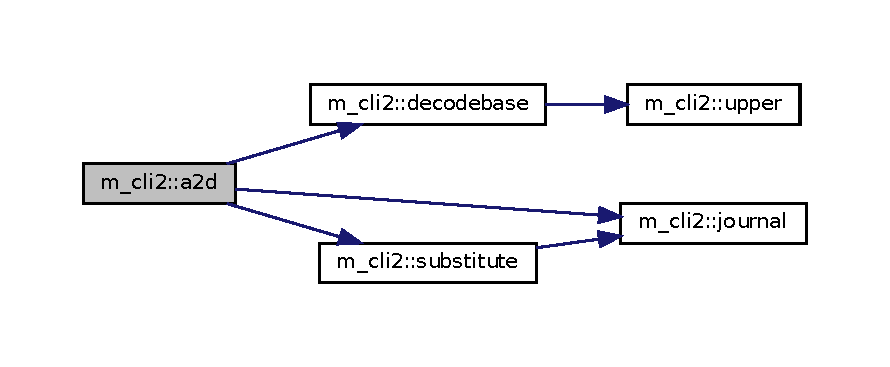
\includegraphics[width=350pt]{namespacem__cli2_ad9e1de0ea9d2b4ed758b2a76bf143bd2_cgraph}
\end{center}
\end{figure}
Here is the caller graph for this function\+:\nopagebreak
\begin{figure}[H]
\begin{center}
\leavevmode
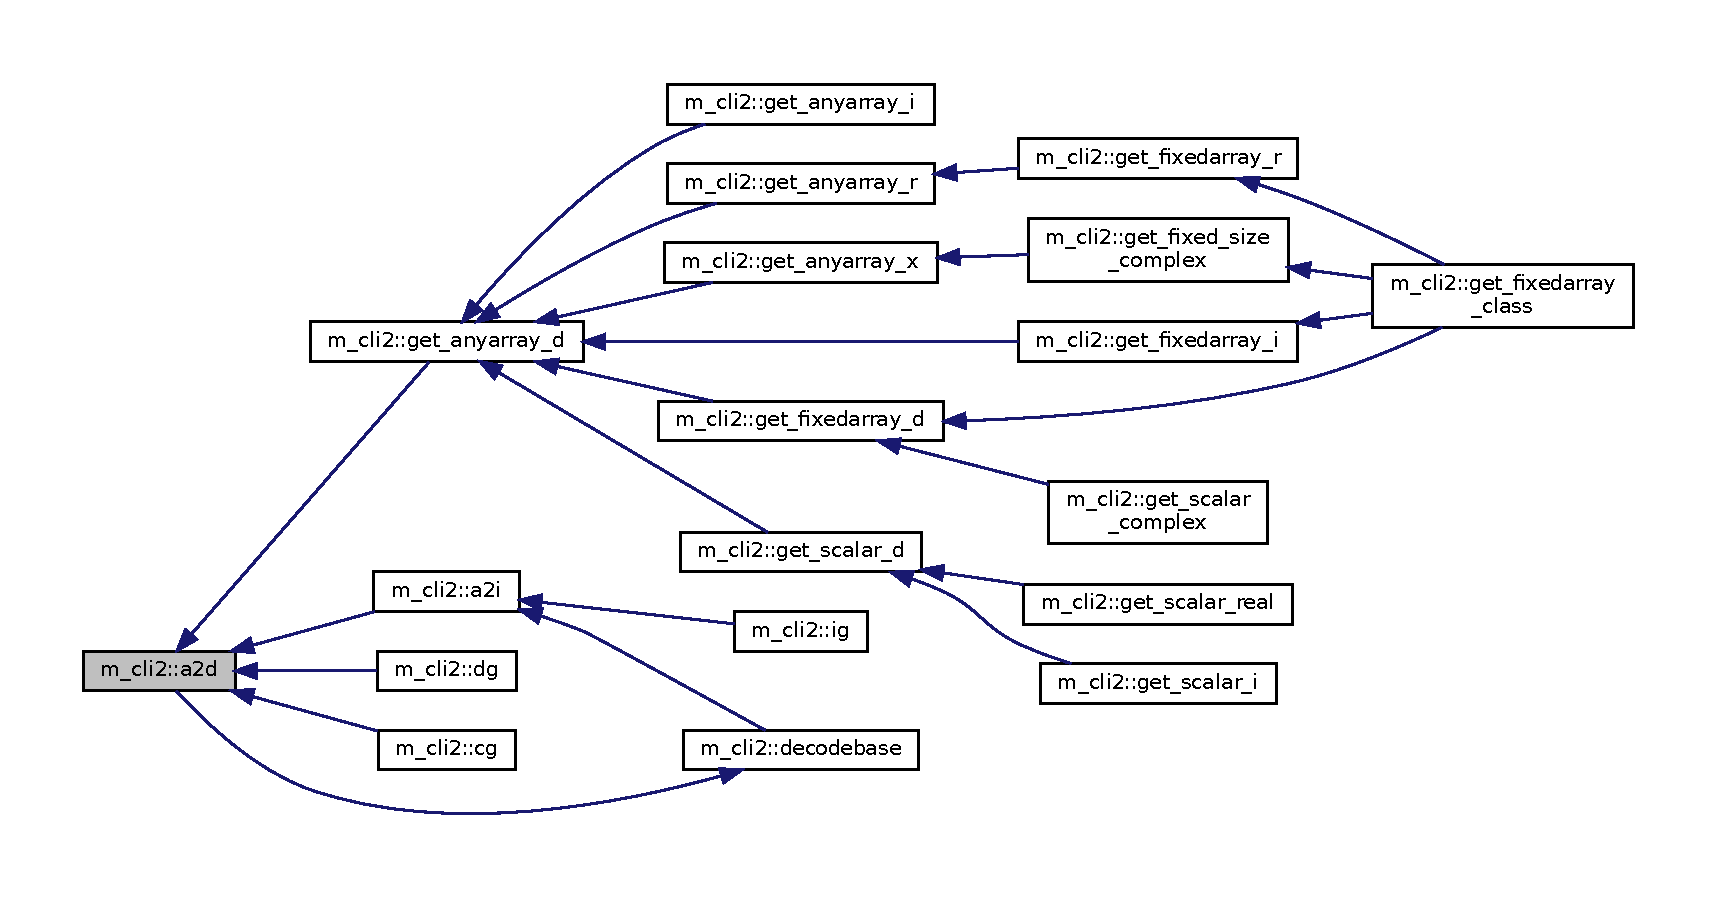
\includegraphics[width=350pt]{namespacem__cli2_ad9e1de0ea9d2b4ed758b2a76bf143bd2_icgraph}
\end{center}
\end{figure}
\mbox{\Hypertarget{namespacem__cli2_a0be58233adafc0bf10dfe69300a05b9f}\label{namespacem__cli2_a0be58233adafc0bf10dfe69300a05b9f}} 
\index{m\_cli2@{m\_cli2}!a2i@{a2i}}
\index{a2i@{a2i}!m\_cli2@{m\_cli2}}
\doxysubsubsection{\texorpdfstring{a2i()}{a2i()}}
{\footnotesize\ttfamily subroutine m\+\_\+cli2\+::a2i (\begin{DoxyParamCaption}\item[{character(len=$\ast$), intent(in)}]{chars,  }\item[{integer, intent(out)}]{valu,  }\item[{integer, intent(out)}]{ierr }\end{DoxyParamCaption})\hspace{0.3cm}{\ttfamily [private]}}



References a2d(), and journal().

Here is the call graph for this function\+:\nopagebreak
\begin{figure}[H]
\begin{center}
\leavevmode
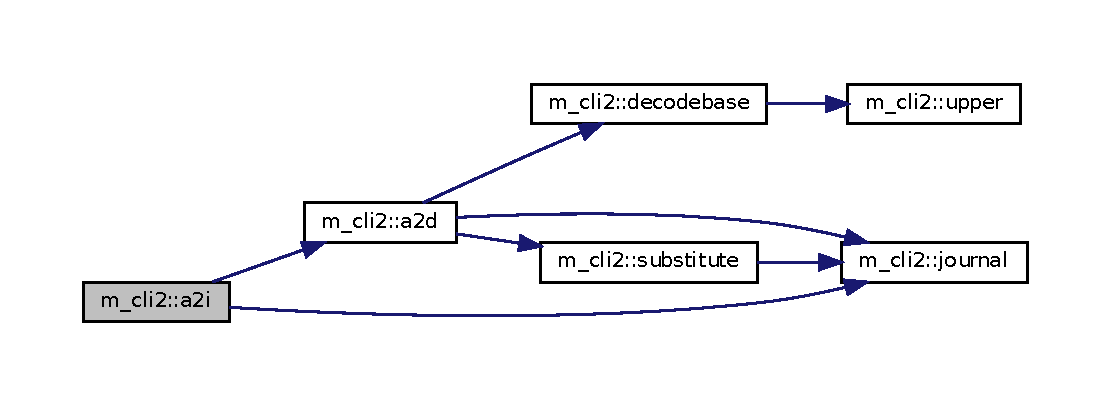
\includegraphics[width=350pt]{namespacem__cli2_a0be58233adafc0bf10dfe69300a05b9f_cgraph}
\end{center}
\end{figure}
Here is the caller graph for this function\+:\nopagebreak
\begin{figure}[H]
\begin{center}
\leavevmode
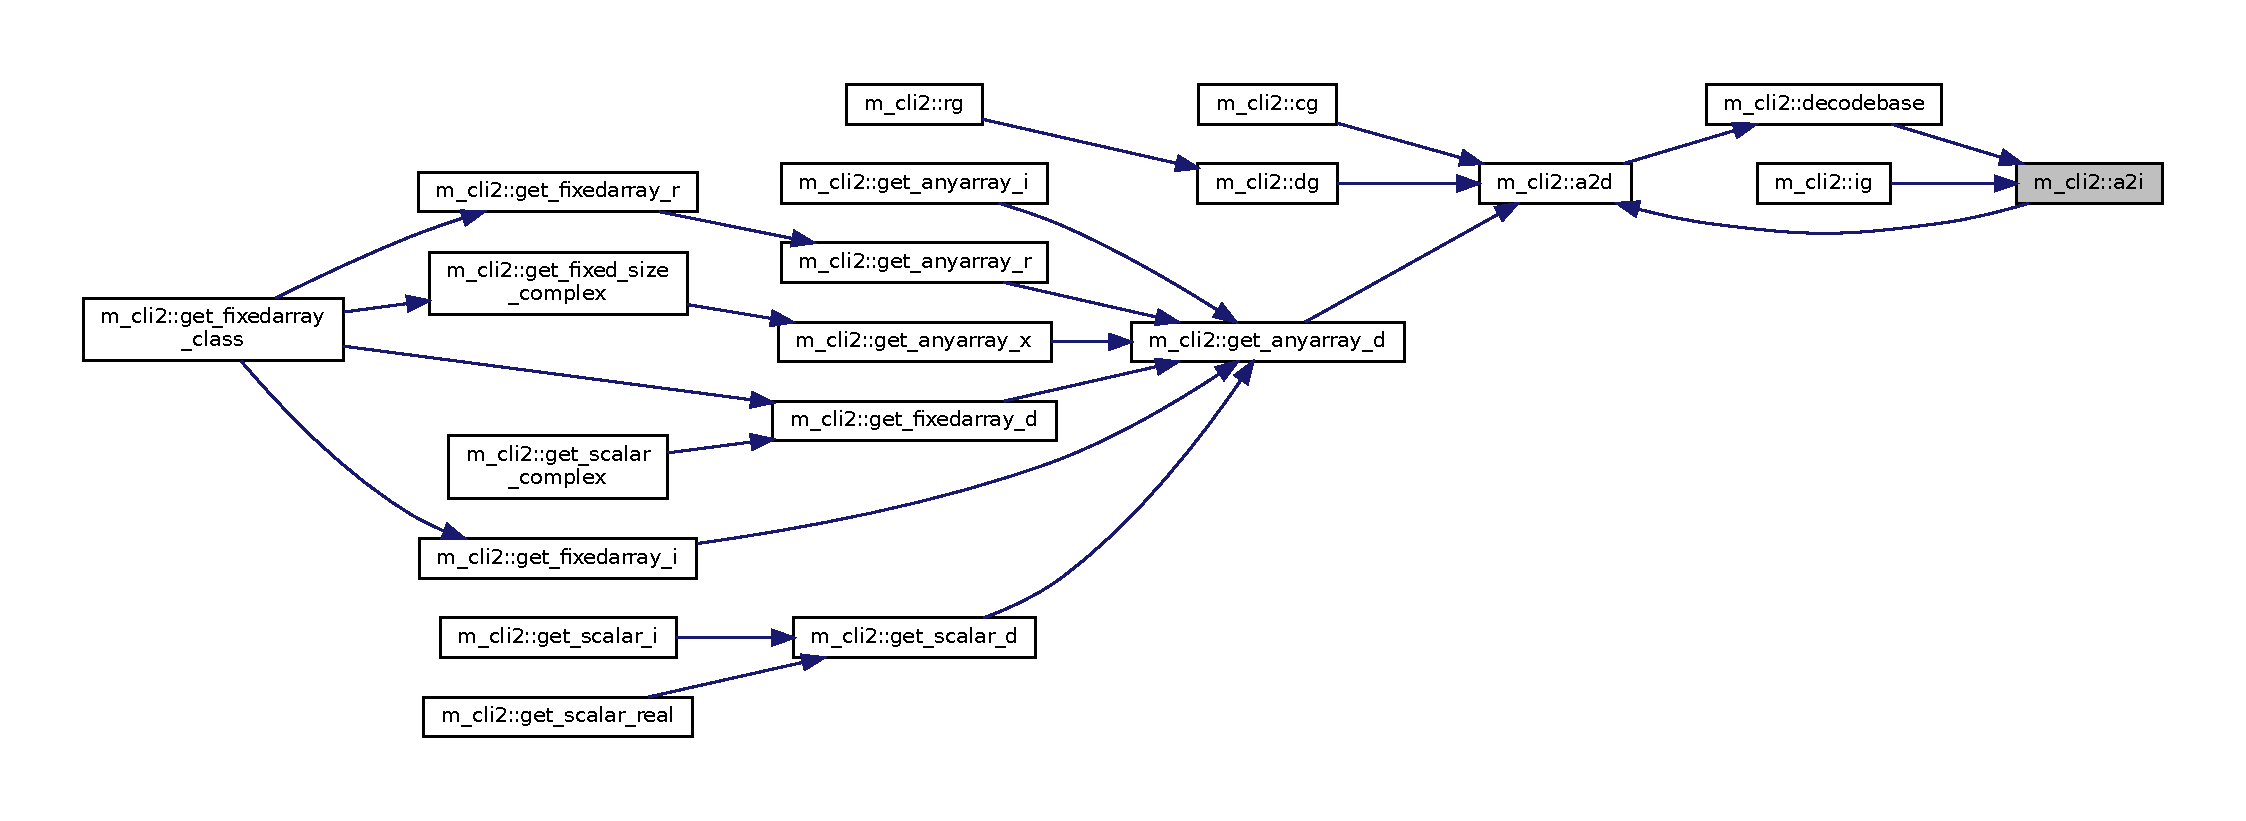
\includegraphics[width=350pt]{namespacem__cli2_a0be58233adafc0bf10dfe69300a05b9f_icgraph}
\end{center}
\end{figure}
\mbox{\Hypertarget{namespacem__cli2_af56d0ddfe2e4b840de521eecae5386e1}\label{namespacem__cli2_af56d0ddfe2e4b840de521eecae5386e1}} 
\index{m\_cli2@{m\_cli2}!atleast@{atleast}}
\index{atleast@{atleast}!m\_cli2@{m\_cli2}}
\doxysubsubsection{\texorpdfstring{atleast()}{atleast()}}
{\footnotesize\ttfamily function m\+\_\+cli2\+::atleast (\begin{DoxyParamCaption}\item[{character(len=$\ast$), intent(in)}]{line,  }\item[{integer, intent(in)}]{length,  }\item[{character(len=$\ast$), intent(in), optional}]{pattern }\end{DoxyParamCaption})\hspace{0.3cm}{\ttfamily [private]}}

Here is the caller graph for this function\+:\nopagebreak
\begin{figure}[H]
\begin{center}
\leavevmode
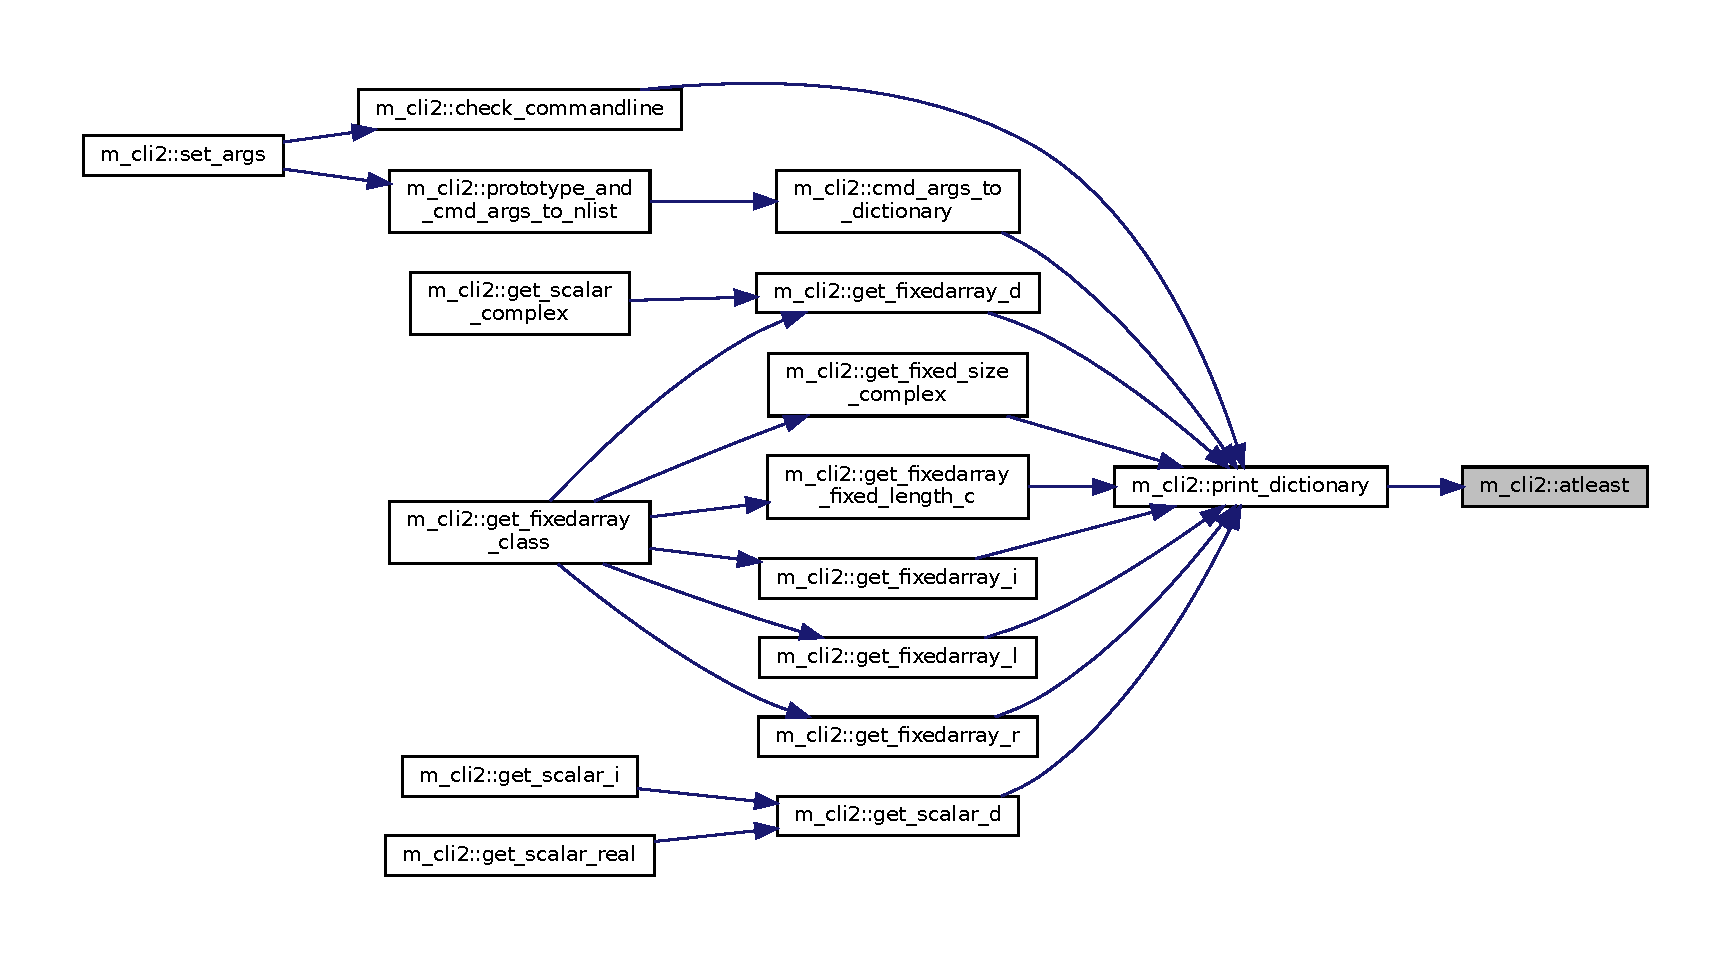
\includegraphics[width=350pt]{namespacem__cli2_af56d0ddfe2e4b840de521eecae5386e1_icgraph}
\end{center}
\end{figure}
\mbox{\Hypertarget{namespacem__cli2_aa611f2b4963a32b3a8667420b146429a}\label{namespacem__cli2_aa611f2b4963a32b3a8667420b146429a}} 
\index{m\_cli2@{m\_cli2}!basename@{basename}}
\index{basename@{basename}!m\_cli2@{m\_cli2}}
\doxysubsubsection{\texorpdfstring{basename()}{basename()}}
{\footnotesize\ttfamily character(\+:) function, allocatable m\+\_\+cli2\+::basename (\begin{DoxyParamCaption}\item[{character($\ast$), intent(in)}]{path,  }\item[{logical, intent(in), optional}]{suffix }\end{DoxyParamCaption})\hspace{0.3cm}{\ttfamily [private]}}



References split().

Here is the call graph for this function\+:\nopagebreak
\begin{figure}[H]
\begin{center}
\leavevmode
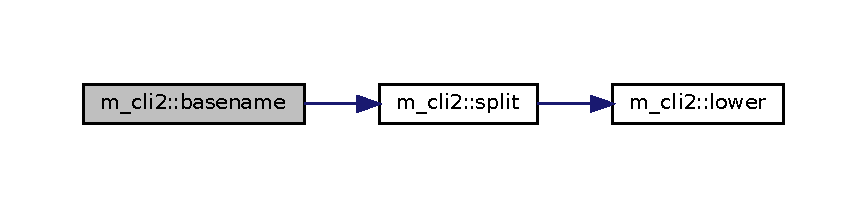
\includegraphics[width=350pt]{namespacem__cli2_aa611f2b4963a32b3a8667420b146429a_cgraph}
\end{center}
\end{figure}
Here is the caller graph for this function\+:\nopagebreak
\begin{figure}[H]
\begin{center}
\leavevmode
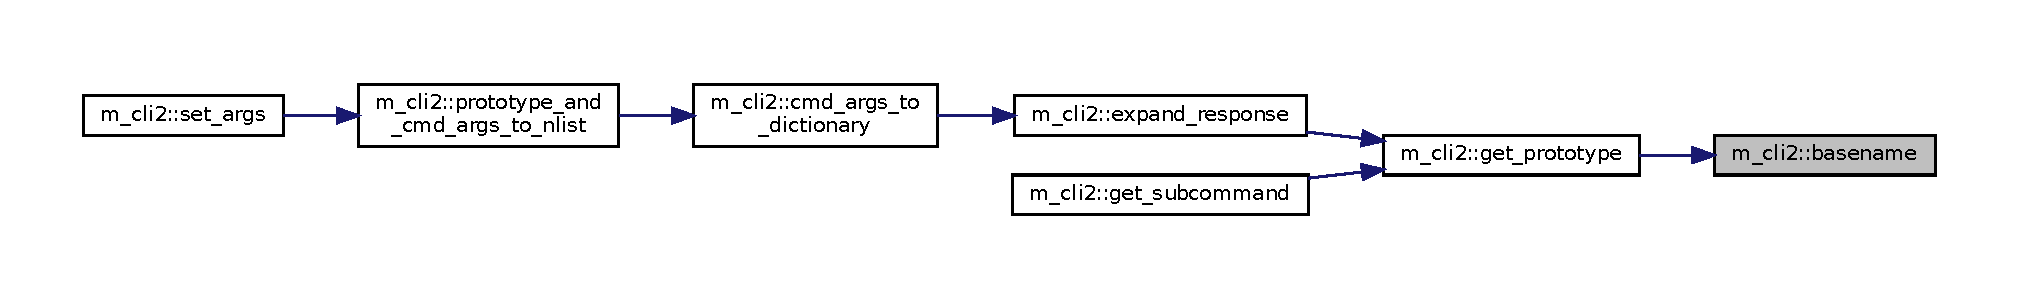
\includegraphics[width=350pt]{namespacem__cli2_aa611f2b4963a32b3a8667420b146429a_icgraph}
\end{center}
\end{figure}
\mbox{\Hypertarget{namespacem__cli2_af45e2401f7c3c2309fe92882c1d5e521}\label{namespacem__cli2_af45e2401f7c3c2309fe92882c1d5e521}} 
\index{m\_cli2@{m\_cli2}!cg@{cg}}
\index{cg@{cg}!m\_cli2@{m\_cli2}}
\doxysubsubsection{\texorpdfstring{cg()}{cg()}}
{\footnotesize\ttfamily complex function, dimension(\+:), allocatable m\+\_\+cli2\+::cg\hspace{0.3cm}{\ttfamily [private]}}



References a2d(), sp, and unnamed.

Here is the call graph for this function\+:\nopagebreak
\begin{figure}[H]
\begin{center}
\leavevmode
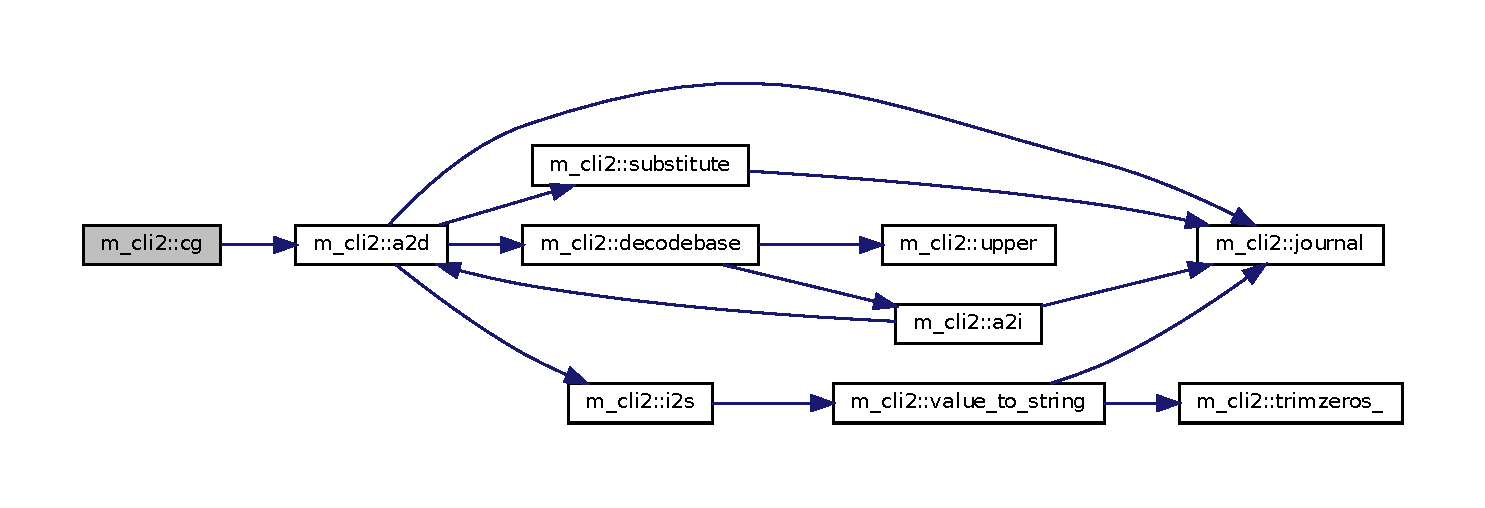
\includegraphics[width=350pt]{namespacem__cli2_af45e2401f7c3c2309fe92882c1d5e521_cgraph}
\end{center}
\end{figure}
\mbox{\Hypertarget{namespacem__cli2_a753fbd0c09fbfd712c7f4add246818cf}\label{namespacem__cli2_a753fbd0c09fbfd712c7f4add246818cf}} 
\index{m\_cli2@{m\_cli2}!cget@{cget}}
\index{cget@{cget}!m\_cli2@{m\_cli2}}
\doxysubsubsection{\texorpdfstring{cget()}{cget()}}
{\footnotesize\ttfamily complex function, public m\+\_\+cli2\+::cget (\begin{DoxyParamCaption}\item[{character(len=$\ast$), intent(in)}]{n }\end{DoxyParamCaption})}

\mbox{\Hypertarget{namespacem__cli2_a05456ce2d696e1632be5efe8e7c2afe3}\label{namespacem__cli2_a05456ce2d696e1632be5efe8e7c2afe3}} 
\index{m\_cli2@{m\_cli2}!cgs@{cgs}}
\index{cgs@{cgs}!m\_cli2@{m\_cli2}}
\doxysubsubsection{\texorpdfstring{cgs()}{cgs()}}
{\footnotesize\ttfamily complex function, dimension(\+:), allocatable m\+\_\+cli2\+::cgs (\begin{DoxyParamCaption}\item[{character(len=$\ast$), intent(in)}]{n }\end{DoxyParamCaption})\hspace{0.3cm}{\ttfamily [private]}}

\mbox{\Hypertarget{namespacem__cli2_ada8b5e7a86778085f55821ec31c5977a}\label{namespacem__cli2_ada8b5e7a86778085f55821ec31c5977a}} 
\index{m\_cli2@{m\_cli2}!check\_commandline@{check\_commandline}}
\index{check\_commandline@{check\_commandline}!m\_cli2@{m\_cli2}}
\doxysubsubsection{\texorpdfstring{check\_commandline()}{check\_commandline()}}
{\footnotesize\ttfamily subroutine, private m\+\_\+cli2\+::check\+\_\+commandline (\begin{DoxyParamCaption}\item[{character(len=\+:), dimension(\+:), intent(in), optional, allocatable}]{help\+\_\+text,  }\item[{character(len=\+:), dimension(\+:), intent(in), optional, allocatable}]{version\+\_\+text }\end{DoxyParamCaption})\hspace{0.3cm}{\ttfamily [private]}}

\hypertarget{namespacem__cli2_autotoc_md6}{}\doxysubsubsection{N\+A\+ME}\label{namespacem__cli2_autotoc_md6}
check\+\_\+commandline(3f) -\/ \mbox{[}A\+R\+G\+U\+M\+E\+N\+TS\+:M\+\_\+\+C\+L\+I2\mbox{]}check command and process pre-\/defined options\hypertarget{namespacem__cli2_autotoc_md7}{}\doxysubsubsection{S\+Y\+N\+O\+P\+S\+IS}\label{namespacem__cli2_autotoc_md7}
\begin{DoxyVerb}  subroutine check_commandline(help_text,version_text,ierr,errmsg)

   character(len=:),allocatable,intent(in),optional :: help_text(:)
   character(len=:),allocatable,intent(in),optional :: version_text(:)
\end{DoxyVerb}
\hypertarget{namespacem__cli2_autotoc_md8}{}\doxysubsubsection{D\+E\+S\+C\+R\+I\+P\+T\+I\+ON}\label{namespacem__cli2_autotoc_md8}
Checks the commandline and processes the implicit --help, --version, --verbose, and --usage parameters.

If the optional text values are supplied they will be displayed by --help and --version command-\/line options, respectively.\hypertarget{namespacem__cli2_autotoc_md9}{}\doxysubsubsection{O\+P\+T\+I\+O\+NS}\label{namespacem__cli2_autotoc_md9}
\begin{DoxyVerb} HELP_TEXT     if present, will be displayed if program is called with
               --help switch, and then the program will terminate. If
               not supplied, the command line initialized string will be
               shown when --help is used on the commandline.

 VERSION_TEXT  if present, will be displayed if program is called with
               --version switch, and then the program will terminate.

    If the first four characters of each line are "@(#)" this prefix
    will not be displayed and the last non-blank letter will be
    removed from each line. This if for support of the SCCS what(1)
    command. If you do not have the what(1) command on GNU/Linux and
    Unix platforms you can probably see how it can be used to place
    metadata in a binary by entering:

     strings demo_commandline|grep '@(#)'|tr '>' '\n'|sed -e 's/  */ /g'
\end{DoxyVerb}
\hypertarget{namespacem__cli2_autotoc_md10}{}\doxysubsubsection{E\+X\+A\+M\+P\+LE}\label{namespacem__cli2_autotoc_md10}
Typical usage\+: \begin{DoxyVerb} program check_commandline
 use M_CLI2,  only : unnamed, set_args, get_args
 implicit none
 integer                      :: i
 character(len=:),allocatable :: version_text(:), help_text(:)
 real               :: x, y, z
 character(len=*),parameter :: cmd='-x 1 -y 2 -z 3'
    version_text=[character(len=80) :: "version 1.0","author: me"]
    help_text=[character(len=80) :: "wish I put instructions","here","I suppose?"]
    call set_args(cmd,help_text,version_text)
    call get_args('x',x,'y',y,'z',z)
    ! All done cracking the command line. Use the values in your program.
    write (*,*)x,y,z
    ! the optional unnamed values on the command line are
    ! accumulated in the character array "UNNAMED"
    if(size(unnamed).gt.0)then
       write (*,'(a)')'files:'
       write (*,'(i6.6,3a)') (i,'[',unnamed(i),']',i=1,size(unnamed))
    endif
 end program check_commandline
\end{DoxyVerb}
 

References debug\+\_\+m\+\_\+cli2, default\+\_\+help(), g\+\_\+quiet, g\+\_\+stop\+\_\+message, gen, get(), journal(), mystop(), and print\+\_\+dictionary().

Here is the call graph for this function\+:\nopagebreak
\begin{figure}[H]
\begin{center}
\leavevmode
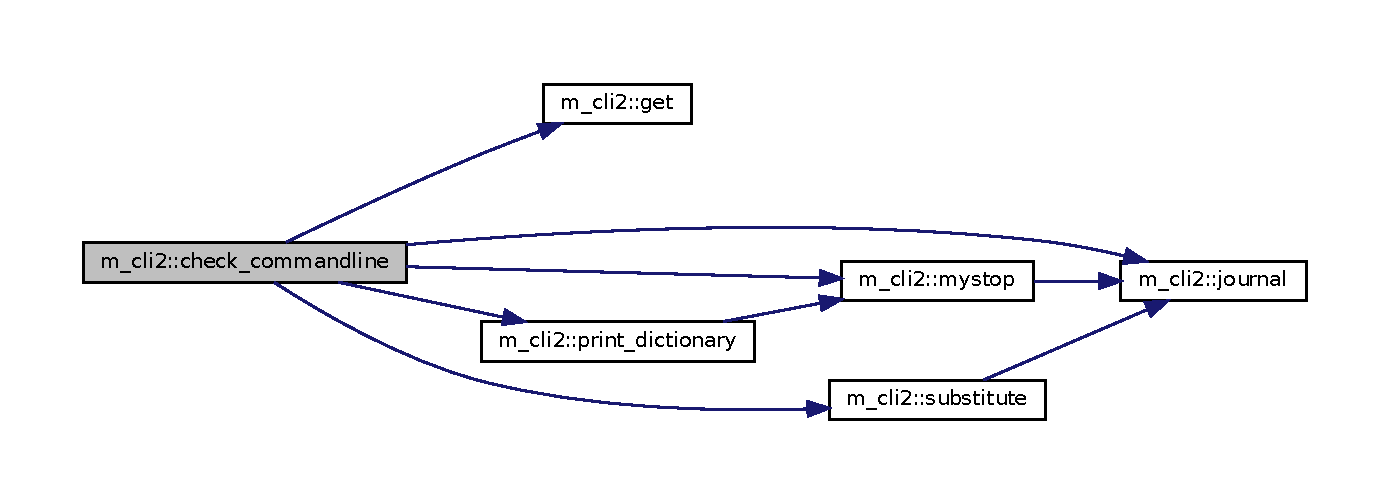
\includegraphics[width=350pt]{namespacem__cli2_ada8b5e7a86778085f55821ec31c5977a_cgraph}
\end{center}
\end{figure}
Here is the caller graph for this function\+:\nopagebreak
\begin{figure}[H]
\begin{center}
\leavevmode
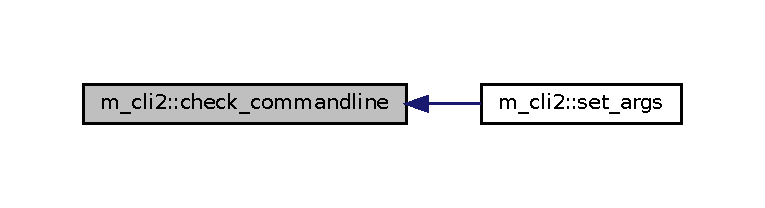
\includegraphics[width=350pt]{namespacem__cli2_ada8b5e7a86778085f55821ec31c5977a_icgraph}
\end{center}
\end{figure}
\mbox{\Hypertarget{namespacem__cli2_a4377e8cb5b593470df7dd8c52cdfc3fd}\label{namespacem__cli2_a4377e8cb5b593470df7dd8c52cdfc3fd}} 
\index{m\_cli2@{m\_cli2}!cmd\_args\_to\_dictionary@{cmd\_args\_to\_dictionary}}
\index{cmd\_args\_to\_dictionary@{cmd\_args\_to\_dictionary}!m\_cli2@{m\_cli2}}
\doxysubsubsection{\texorpdfstring{cmd\_args\_to\_dictionary()}{cmd\_args\_to\_dictionary()}}
{\footnotesize\ttfamily subroutine m\+\_\+cli2\+::cmd\+\_\+args\+\_\+to\+\_\+dictionary\hspace{0.3cm}{\ttfamily [private]}}



References args, debug\+\_\+m\+\_\+cli2, expand\+\_\+response(), g\+\_\+keyword\+\_\+single\+\_\+letter, g\+\_\+remaining, g\+\_\+remaining\+\_\+on, g\+\_\+remaining\+\_\+option\+\_\+allowed, g\+\_\+response, g\+\_\+strict, gen, get(), get\+\_\+next\+\_\+argument(), ifnull(), keywords, locate\+\_\+key(), mandatory, mystop(), print\+\_\+dictionary(), quote(), unnamed, update(), and upper().

Here is the call graph for this function\+:\nopagebreak
\begin{figure}[H]
\begin{center}
\leavevmode
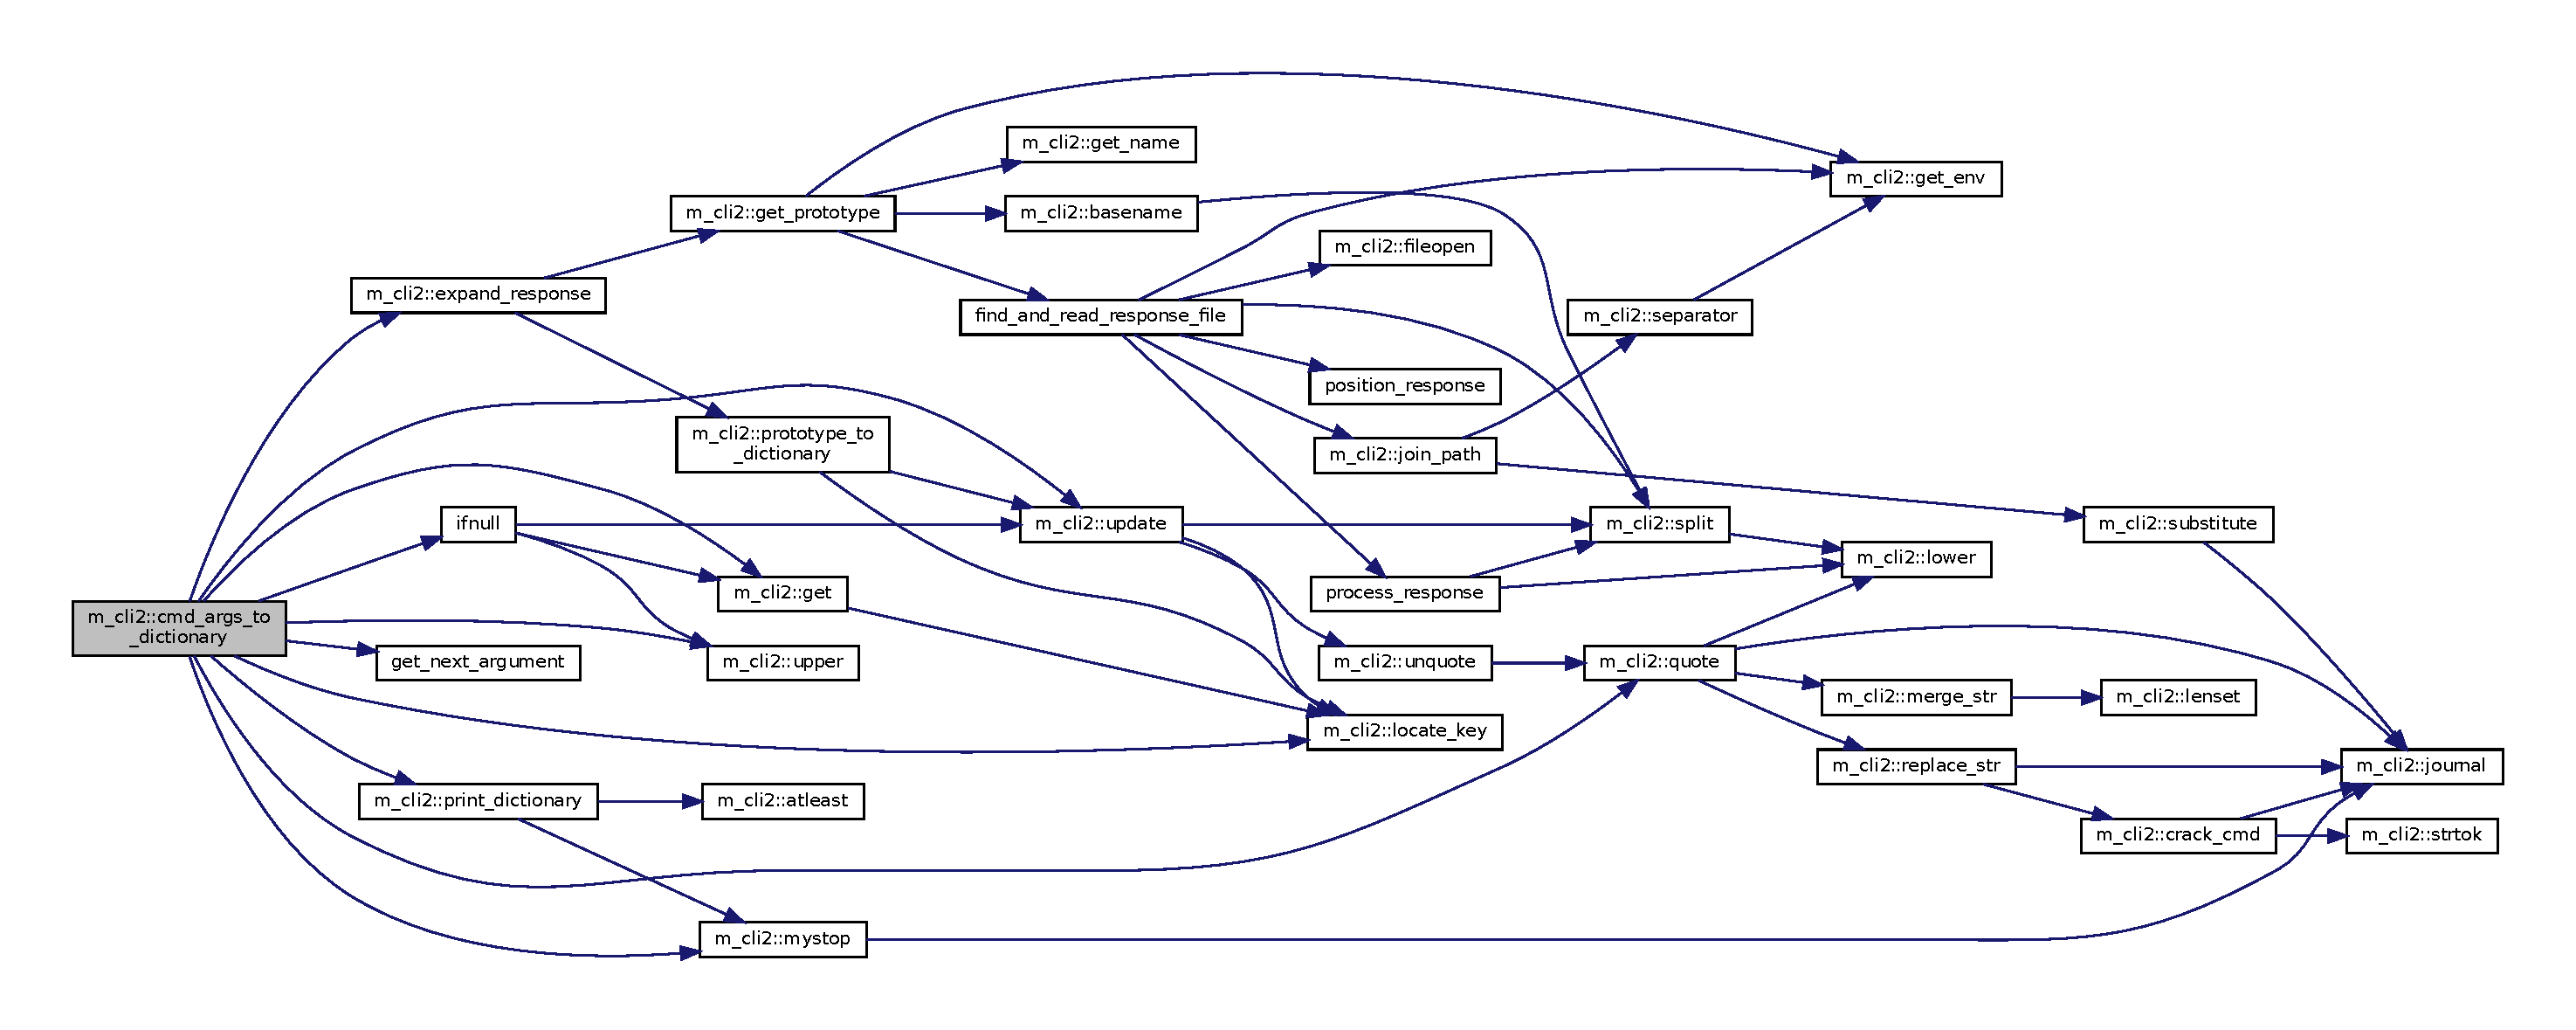
\includegraphics[width=350pt]{namespacem__cli2_a4377e8cb5b593470df7dd8c52cdfc3fd_cgraph}
\end{center}
\end{figure}
Here is the caller graph for this function\+:\nopagebreak
\begin{figure}[H]
\begin{center}
\leavevmode
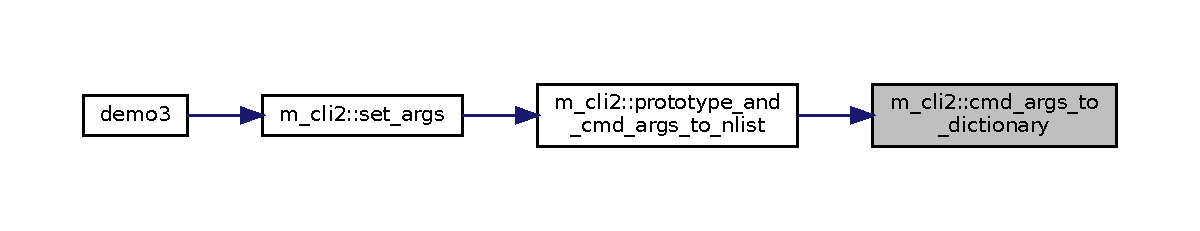
\includegraphics[width=350pt]{namespacem__cli2_a4377e8cb5b593470df7dd8c52cdfc3fd_icgraph}
\end{center}
\end{figure}
\mbox{\Hypertarget{namespacem__cli2_a710b26995119aee101959555b1bac8e2}\label{namespacem__cli2_a710b26995119aee101959555b1bac8e2}} 
\index{m\_cli2@{m\_cli2}!crack\_cmd@{crack\_cmd}}
\index{crack\_cmd@{crack\_cmd}!m\_cli2@{m\_cli2}}
\doxysubsubsection{\texorpdfstring{crack\_cmd()}{crack\_cmd()}}
{\footnotesize\ttfamily subroutine m\+\_\+cli2\+::crack\+\_\+cmd (\begin{DoxyParamCaption}\item[{character(len=$\ast$), intent(in)}]{cmd,  }\item[{character(len=\+:), intent(out), allocatable}]{old,  }\item[{character(len=\+:), intent(out), allocatable}]{new,  }\item[{integer}]{ierr }\end{DoxyParamCaption})\hspace{0.3cm}{\ttfamily [private]}}

\hypertarget{namespacem__cli2_autotoc_md130}{}\doxysubsubsection{N\+A\+ME}\label{namespacem__cli2_autotoc_md130}
replace\+\_\+str(3f) -\/ \mbox{[}M\+\_\+\+C\+L\+I2\+:E\+D\+I\+T\+I\+NG\mbox{]} function globally replaces one substring for another in string (L\+I\+C\+E\+N\+SE\+:PD)\hypertarget{namespacem__cli2_autotoc_md131}{}\doxysubsubsection{S\+Y\+N\+O\+P\+S\+IS}\label{namespacem__cli2_autotoc_md131}
\begin{DoxyVerb}function replace_str(targetline[,old,new|cmd],range,ierr) result (newline)

 character(len=*)                       :: targetline
 character(len=*),intent(in),optional   :: old
 character(len=*),intent(in),optional   :: new
 character(len=*),intent(in),optional   :: cmd
 integer,intent(in),optional            :: range(2)
 integer,intent(out),optional           :: ierr
 logical,intent(in),optional            :: clip
 character(len=:),allocatable           :: newline
\end{DoxyVerb}
 \hypertarget{namespacem__cli2_autotoc_md132}{}\doxysubsubsection{D\+E\+S\+C\+R\+I\+P\+T\+I\+ON}\label{namespacem__cli2_autotoc_md132}
Globally replace one substring for another in string. Either C\+MD or O\+LD and N\+EW must be specified.\hypertarget{namespacem__cli2_autotoc_md133}{}\doxysubsubsection{O\+P\+T\+I\+O\+NS}\label{namespacem__cli2_autotoc_md133}
targetline input line to be changed old old substring to replace new new substring cmd alternate way to specify old and new string, in the form c/old/new/; where \char`\"{}/\char`\"{} can be any character not in \char`\"{}old\char`\"{} or \char`\"{}new\char`\"{} range if present, only change range(1) to range(2) of occurrences of old string ierr error code. iF ier = -\/1 bad directive, $>$= 0 then count of changes made clip whether to return trailing spaces or not. Defaults to .false. \hypertarget{namespacem__cli2_autotoc_md134}{}\doxysubsubsection{R\+E\+T\+U\+R\+NS}\label{namespacem__cli2_autotoc_md134}
newline allocatable string returned\hypertarget{namespacem__cli2_autotoc_md135}{}\doxysubsubsection{E\+X\+A\+M\+P\+L\+ES}\label{namespacem__cli2_autotoc_md135}
Sample Program\+: \begin{DoxyVerb}  program demo_replace_str
  use M_CLI2, only : replace_str
  implicit none
  character(len=:),allocatable :: targetline

  targetline='this is the input string'

  call testit('th','TH','THis is THe input string')

  ! a null old substring means "at beginning of line"
  call testit('','BEFORE:', 'BEFORE:THis is THe input string')

  ! a null new string deletes occurrences of the old substring
  call testit('i','', 'BEFORE:THs s THe nput strng')

  write(*,*)'Examples of the use of RANGE='

  targetline=replace_str('a b ab baaa aaaa','a','A')
  write(*,*)'replace a with A ['//targetline//']'

  targetline=replace_str('a b ab baaa aaaa','a','A',range=[3,5])
  write(*,*)'replace a with A instances 3 to 5 ['//targetline//']'

  targetline=replace_str('a b ab baaa aaaa','a','',range=[3,5])
  write(*,*)'replace a with null instances 3 to 5 ['//targetline//']'

  targetline=replace_str('a b ab baaa aaaa aa aa a a a aa aaaaaa','aa','CCCC',range=[3,5])
  write(*,*)'replace aa with CCCC instances 3 to 5 ['//targetline//']'

  contains
  subroutine testit(old,new,expected)
  character(len=*),intent(in) :: old,new,expected
  write(*,*)repeat('=',79)
  write(*,*)':STARTED ['//targetline//']'
  write(*,*)':OLD['//old//']', ' NEW['//new//']'
  targetline=replace_str(targetline,old,new)
  write(*,*)':GOT     ['//targetline//']'
  write(*,*)':EXPECTED['//expected//']'
  write(*,*)':TEST    [',targetline.eq.expected,']'
  end subroutine testit

  end program demo_replace_str
\end{DoxyVerb}


Expected output

\DoxyHorRuler{0}
 S\+T\+A\+R\+T\+ED \mbox{[}this is the input string\mbox{]} O\+LD\mbox{[}th\mbox{]} N\+EW\mbox{[}TH\mbox{]} G\+OT \mbox{[}T\+His is T\+He input string\mbox{]} E\+X\+P\+E\+C\+T\+ED\mbox{[}T\+His is T\+He input string\mbox{]} \hypertarget{namespacem__cli2_autotoc_md137}{}\doxysubsection{T\+E\+S\+T    \mbox{[} T \mbox{]}}\label{namespacem__cli2_autotoc_md137}
S\+T\+A\+R\+T\+ED \mbox{[}T\+His is T\+He input string\mbox{]} O\+LD\mbox{[}\mbox{]} N\+EW\mbox{[}B\+E\+F\+O\+RE\+:\mbox{]} G\+OT \mbox{[}B\+E\+F\+O\+RE\+:T\+His is T\+He input string\mbox{]} E\+X\+P\+E\+C\+T\+ED\mbox{[}B\+E\+F\+O\+RE\+:T\+His is T\+He input string\mbox{]} \hypertarget{namespacem__cli2_autotoc_md138}{}\doxysubsection{T\+E\+S\+T    \mbox{[} T \mbox{]}}\label{namespacem__cli2_autotoc_md138}
S\+T\+A\+R\+T\+ED \mbox{[}B\+E\+F\+O\+RE\+:T\+His is T\+He input string\mbox{]} O\+LD\mbox{[}i\mbox{]} N\+EW\mbox{[}\mbox{]} G\+OT \mbox{[}B\+E\+F\+O\+RE\+:T\+Hs s T\+He nput strng\mbox{]} E\+X\+P\+E\+C\+T\+ED\mbox{[}B\+E\+F\+O\+RE\+:T\+Hs s T\+He nput strng\mbox{]} T\+E\+ST \mbox{[} T \mbox{]} Examples of the use of R\+A\+N\+GE= replace a with A \mbox{[}A b Ab b\+A\+AA A\+A\+AA\mbox{]} replace a with A instances 3 to 5 \mbox{[}a b ab b\+A\+AA aaaa\mbox{]} replace a with null instances 3 to 5 \mbox{[}a b ab b aaaa\mbox{]} replace aa with C\+C\+CC instances 3 to 5 \mbox{[}a b ab baaa aa\+C\+C\+CC C\+C\+CC C\+C\+CC a a a aa aaaaaa\mbox{]}\hypertarget{namespacem__cli2_autotoc_md139}{}\doxysubsubsection{A\+U\+T\+H\+OR}\label{namespacem__cli2_autotoc_md139}
John S. Urban \hypertarget{namespacem__cli2_autotoc_md140}{}\doxysubsubsection{L\+I\+C\+E\+N\+SE}\label{namespacem__cli2_autotoc_md140}
Public Domain 

References journal(), and strtok().

Here is the call graph for this function\+:\nopagebreak
\begin{figure}[H]
\begin{center}
\leavevmode
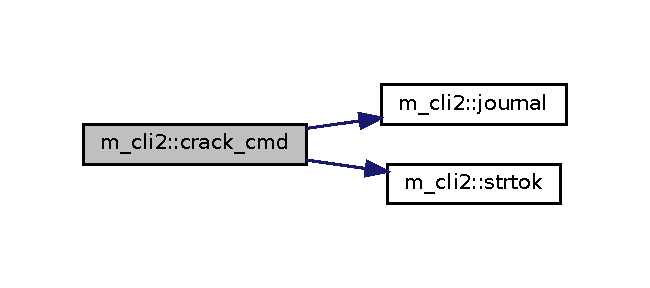
\includegraphics[width=312pt]{namespacem__cli2_a710b26995119aee101959555b1bac8e2_cgraph}
\end{center}
\end{figure}
Here is the caller graph for this function\+:\nopagebreak
\begin{figure}[H]
\begin{center}
\leavevmode
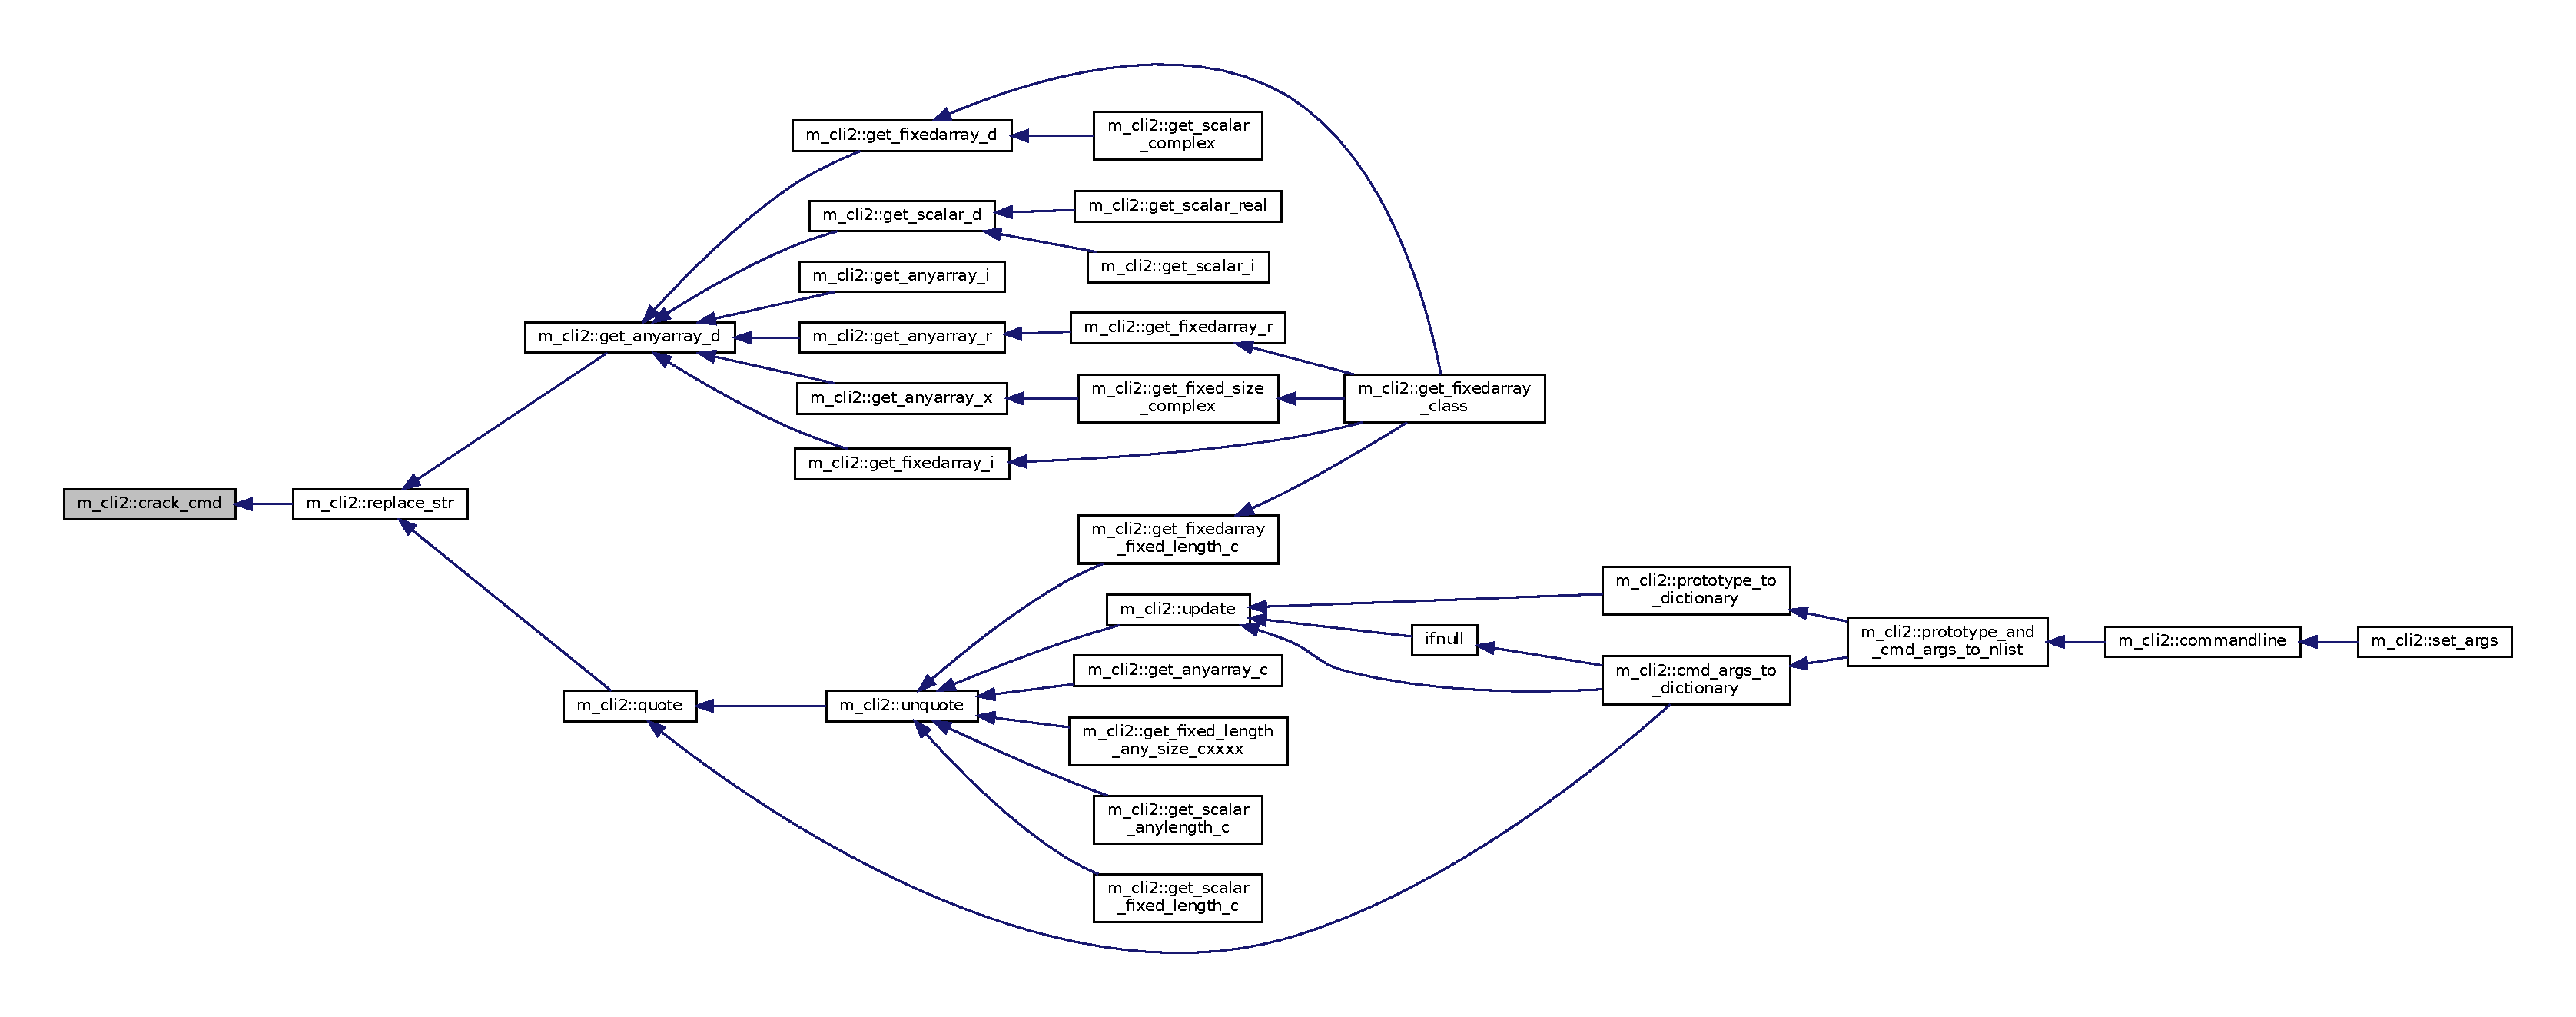
\includegraphics[width=350pt]{namespacem__cli2_a710b26995119aee101959555b1bac8e2_icgraph}
\end{center}
\end{figure}
\mbox{\Hypertarget{namespacem__cli2_a1029304d495b2bf791e03cfab5983bbb}\label{namespacem__cli2_a1029304d495b2bf791e03cfab5983bbb}} 
\index{m\_cli2@{m\_cli2}!decodebase@{decodebase}}
\index{decodebase@{decodebase}!m\_cli2@{m\_cli2}}
\doxysubsubsection{\texorpdfstring{decodebase()}{decodebase()}}
{\footnotesize\ttfamily logical function m\+\_\+cli2\+::decodebase (\begin{DoxyParamCaption}\item[{character(len=$\ast$), intent(in)}]{string,  }\item[{integer, intent(in)}]{basein,  }\item[{integer, intent(out)}]{out\+\_\+baseten }\end{DoxyParamCaption})\hspace{0.3cm}{\ttfamily [private]}}

\hypertarget{namespacem__cli2_autotoc_md165}{}\doxysubsubsection{N\+A\+ME}\label{namespacem__cli2_autotoc_md165}
\begin{DoxyVerb}decodebase(3f) - [M_CLI2:BASE] convert whole number string in base [2-36] to base 10 number
(LICENSE:PD)
\end{DoxyVerb}
\hypertarget{namespacem__cli2_autotoc_md166}{}\doxysubsubsection{S\+Y\+N\+O\+P\+S\+IS}\label{namespacem__cli2_autotoc_md166}
logical function decodebase(string,basein,out10)

character(len=$\ast$),intent(in) \+:: string integer,intent(in) \+:: basein integer,intent(out) \+:: out10 \hypertarget{namespacem__cli2_autotoc_md167}{}\doxysubsubsection{D\+E\+S\+C\+R\+I\+P\+T\+I\+ON}\label{namespacem__cli2_autotoc_md167}
\begin{DoxyVerb}Convert a numeric string representing a whole number in base BASEIN
to base 10. The function returns FALSE if BASEIN is not in the range
[2..36] or if string STRING contains invalid characters in base BASEIN
or if result OUT10 is too big

The letters A,B,...,Z represent 10,11,...,36 in the base > 10.
\end{DoxyVerb}
\hypertarget{namespacem__cli2_autotoc_md168}{}\doxysubsubsection{O\+P\+T\+I\+O\+NS}\label{namespacem__cli2_autotoc_md168}
string input string. It represents a whole number in the base specified by B\+A\+S\+E\+IN unless B\+A\+S\+E\+IN is set to zero. When B\+A\+S\+E\+IN is zero S\+T\+R\+I\+NG is assumed to be of the form B\+A\+S\+E\+::\+V\+A\+L\+UE where B\+A\+SE represents the function normally provided by B\+A\+S\+E\+IN. basein base of input string; either 0 or from 2 to 36. out10 output value in base 10\hypertarget{namespacem__cli2_autotoc_md169}{}\doxysubsubsection{E\+X\+A\+M\+P\+LE}\label{namespacem__cli2_autotoc_md169}
Sample program\+: \begin{DoxyVerb} program demo_decodebase
 use M_CLI2, only : codebase, decodebase
 implicit none
 integer           :: ba,bd
 character(len=40) :: x,y
 integer           :: r

 print *,' BASE CONVERSION'
 write(*,'("Start   Base (2 to 36): ")',advance='no'); read *, bd
 write(*,'("Arrival Base (2 to 36): ")',advance='no'); read *, ba
 INFINITE: do
    print *,''
    write(*,'("Enter number in start base: ")',advance='no'); read *, x
    if(x.eq.'0') exit INFINITE
    if(decodebase(x,bd,r)) then
       if(codebase(r,ba,y)) then
         write(*,'("In base ",I2,": ",A20)')  ba, y
       else
         print *,'Error in coding number.'
       endif
    else
       print *,'Error in decoding number.'
    endif
 enddo INFINITE

 end program demo_decodebase
\end{DoxyVerb}
\hypertarget{namespacem__cli2_autotoc_md170}{}\doxysubsubsection{A\+U\+T\+H\+OR}\label{namespacem__cli2_autotoc_md170}
John S. Urban

Ref.\+: "Math matiques en Turbo-\/\+Pascal by M. Ducamp and A. Reverchon (2), Eyrolles, Paris, 1988".

based on a F90 Version By J-\/P Moreau (www.\+jpmoreau.\+fr)\hypertarget{namespacem__cli2_autotoc_md171}{}\doxysubsubsection{L\+I\+C\+E\+N\+SE}\label{namespacem__cli2_autotoc_md171}
Public Domain 

References a2i(), and upper().

Here is the call graph for this function\+:\nopagebreak
\begin{figure}[H]
\begin{center}
\leavevmode
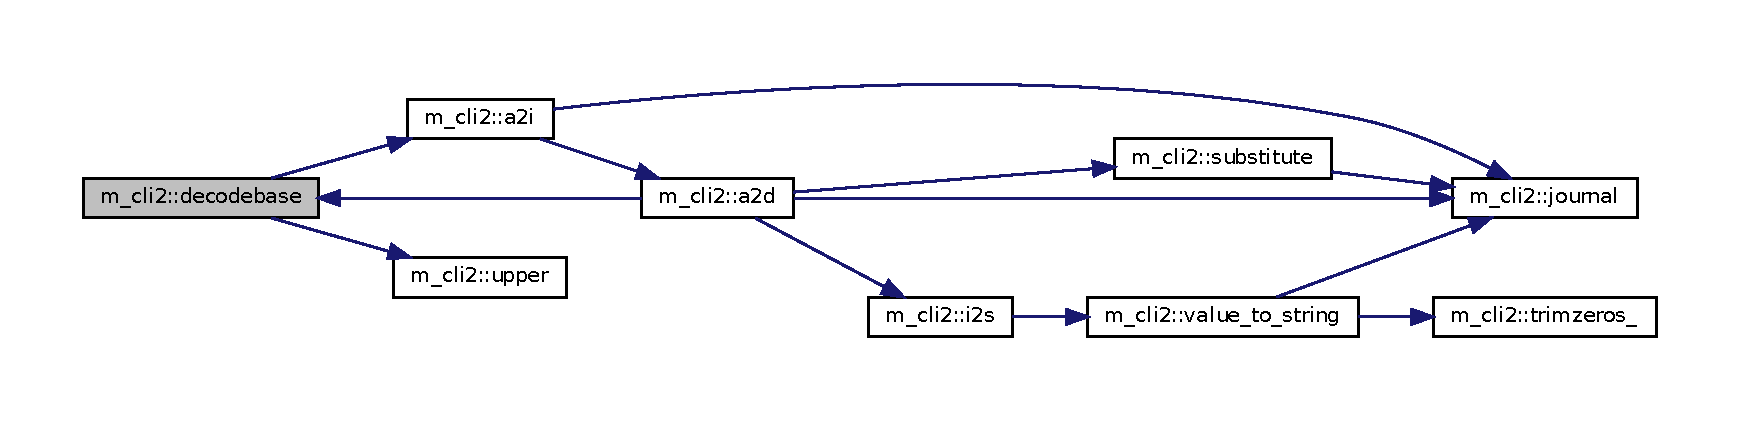
\includegraphics[width=350pt]{namespacem__cli2_a1029304d495b2bf791e03cfab5983bbb_cgraph}
\end{center}
\end{figure}
Here is the caller graph for this function\+:\nopagebreak
\begin{figure}[H]
\begin{center}
\leavevmode
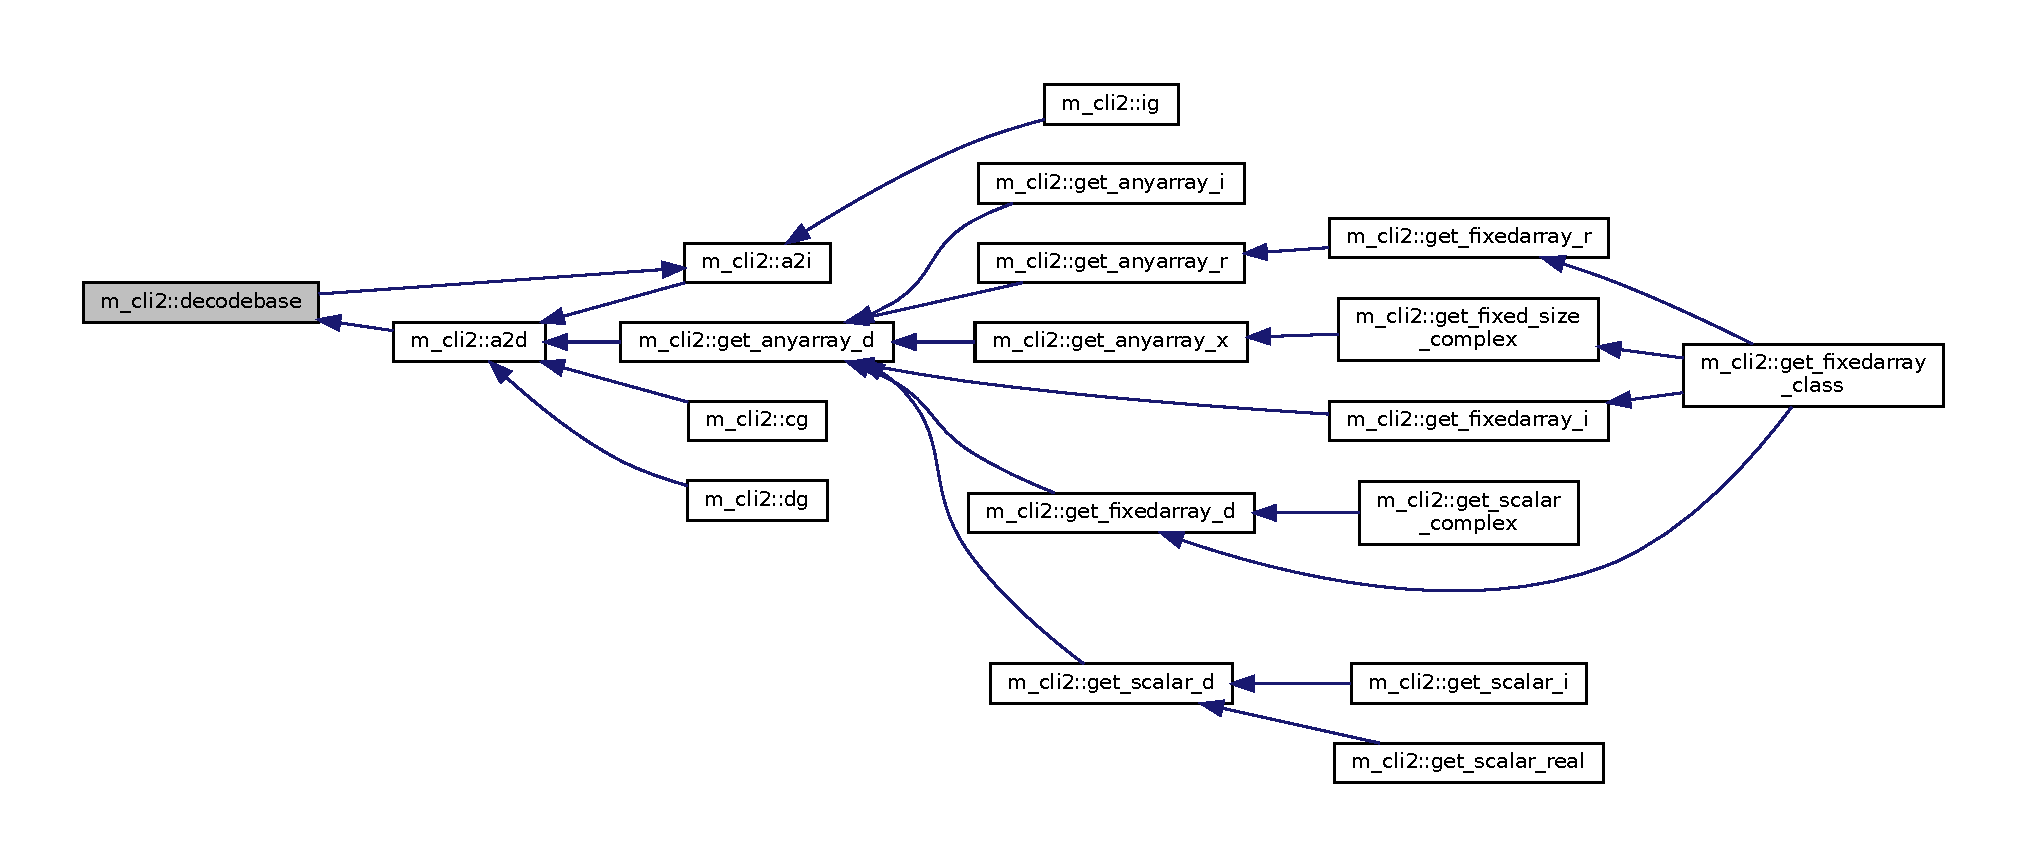
\includegraphics[width=350pt]{namespacem__cli2_a1029304d495b2bf791e03cfab5983bbb_icgraph}
\end{center}
\end{figure}
\mbox{\Hypertarget{namespacem__cli2_a06ddc2533e5122b8f898bae7db0fea87}\label{namespacem__cli2_a06ddc2533e5122b8f898bae7db0fea87}} 
\index{m\_cli2@{m\_cli2}!dg@{dg}}
\index{dg@{dg}!m\_cli2@{m\_cli2}}
\doxysubsubsection{\texorpdfstring{dg()}{dg()}}
{\footnotesize\ttfamily real(kind=\mbox{\hyperlink{namespacem__cli2_acf83f1963cf6a56ad0221cfcf5402440}{dp}}) function, dimension(\+:), allocatable m\+\_\+cli2\+::dg\hspace{0.3cm}{\ttfamily [private]}}



References a2d(), and unnamed.

Here is the call graph for this function\+:\nopagebreak
\begin{figure}[H]
\begin{center}
\leavevmode
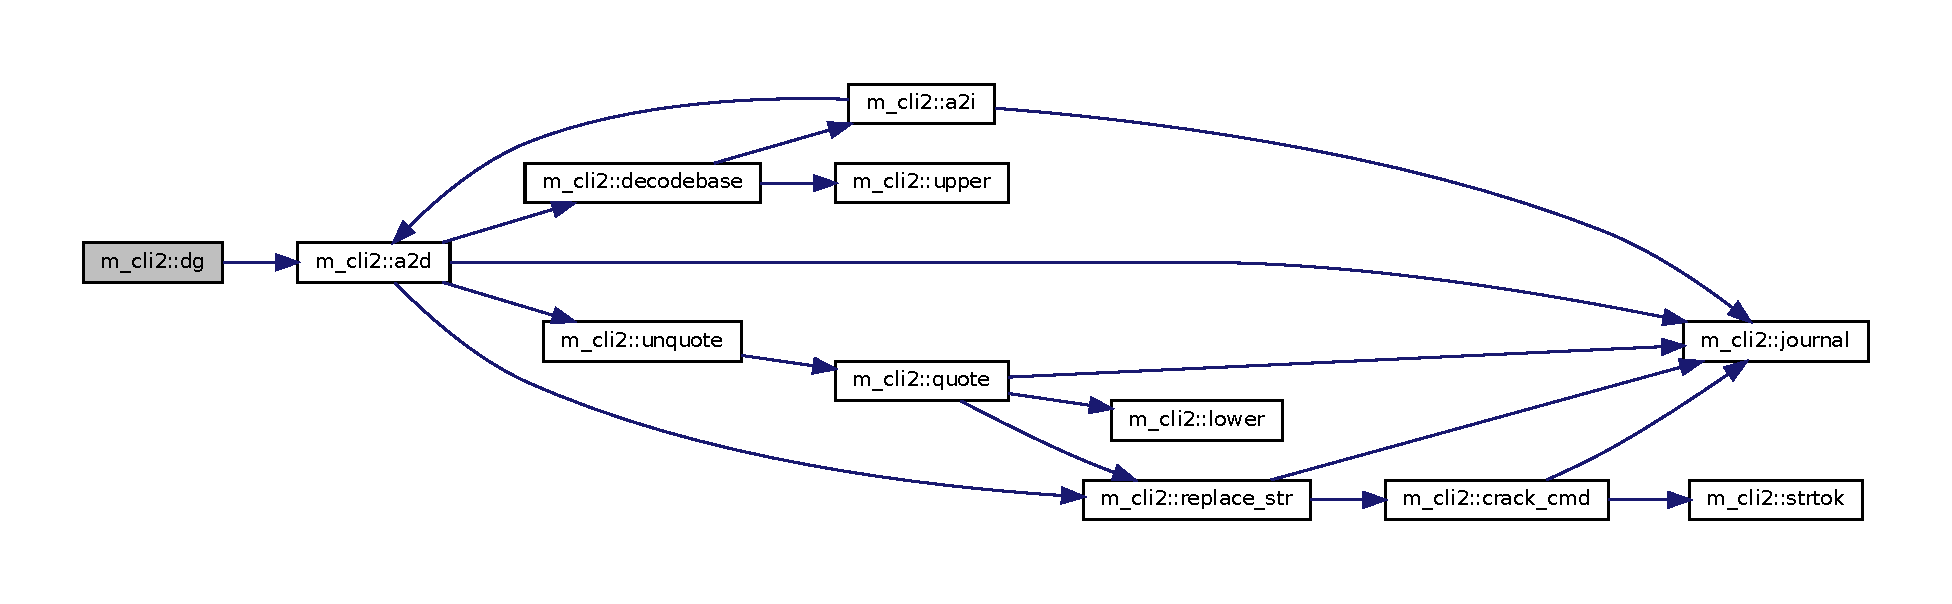
\includegraphics[width=350pt]{namespacem__cli2_a06ddc2533e5122b8f898bae7db0fea87_cgraph}
\end{center}
\end{figure}
Here is the caller graph for this function\+:\nopagebreak
\begin{figure}[H]
\begin{center}
\leavevmode
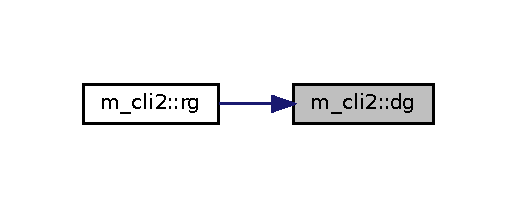
\includegraphics[width=248pt]{namespacem__cli2_a06ddc2533e5122b8f898bae7db0fea87_icgraph}
\end{center}
\end{figure}
\mbox{\Hypertarget{namespacem__cli2_abb63058af19a47e19a78567c4a320c16}\label{namespacem__cli2_abb63058af19a47e19a78567c4a320c16}} 
\index{m\_cli2@{m\_cli2}!dget@{dget}}
\index{dget@{dget}!m\_cli2@{m\_cli2}}
\doxysubsubsection{\texorpdfstring{dget()}{dget()}}
{\footnotesize\ttfamily real(kind=\mbox{\hyperlink{namespacem__cli2_acf83f1963cf6a56ad0221cfcf5402440}{dp}}) function, public m\+\_\+cli2\+::dget (\begin{DoxyParamCaption}\item[{character(len=$\ast$), intent(in)}]{n }\end{DoxyParamCaption})}

\mbox{\Hypertarget{namespacem__cli2_a84bc83f5e8ec87f4d691e40df7569c83}\label{namespacem__cli2_a84bc83f5e8ec87f4d691e40df7569c83}} 
\index{m\_cli2@{m\_cli2}!dgs@{dgs}}
\index{dgs@{dgs}!m\_cli2@{m\_cli2}}
\doxysubsubsection{\texorpdfstring{dgs()}{dgs()}}
{\footnotesize\ttfamily real(kind=\mbox{\hyperlink{namespacem__cli2_acf83f1963cf6a56ad0221cfcf5402440}{dp}}) function, dimension(\+:), allocatable m\+\_\+cli2\+::dgs (\begin{DoxyParamCaption}\item[{character(len=$\ast$), intent(in)}]{n }\end{DoxyParamCaption})\hspace{0.3cm}{\ttfamily [private]}}

\mbox{\Hypertarget{namespacem__cli2_a98df7b928a09462fa32a10931acf157c}\label{namespacem__cli2_a98df7b928a09462fa32a10931acf157c}} 
\index{m\_cli2@{m\_cli2}!expand\_response@{expand\_response}}
\index{expand\_response@{expand\_response}!m\_cli2@{m\_cli2}}
\doxysubsubsection{\texorpdfstring{expand\_response()}{expand\_response()}}
{\footnotesize\ttfamily subroutine m\+\_\+cli2\+::expand\+\_\+response (\begin{DoxyParamCaption}\item[{character(len=$\ast$), intent(in)}]{name }\end{DoxyParamCaption})\hspace{0.3cm}{\ttfamily [private]}}



References debug\+\_\+m\+\_\+cli2, g\+\_\+append, gen, get\+\_\+prototype(), and prototype\+\_\+to\+\_\+dictionary().

Here is the call graph for this function\+:\nopagebreak
\begin{figure}[H]
\begin{center}
\leavevmode
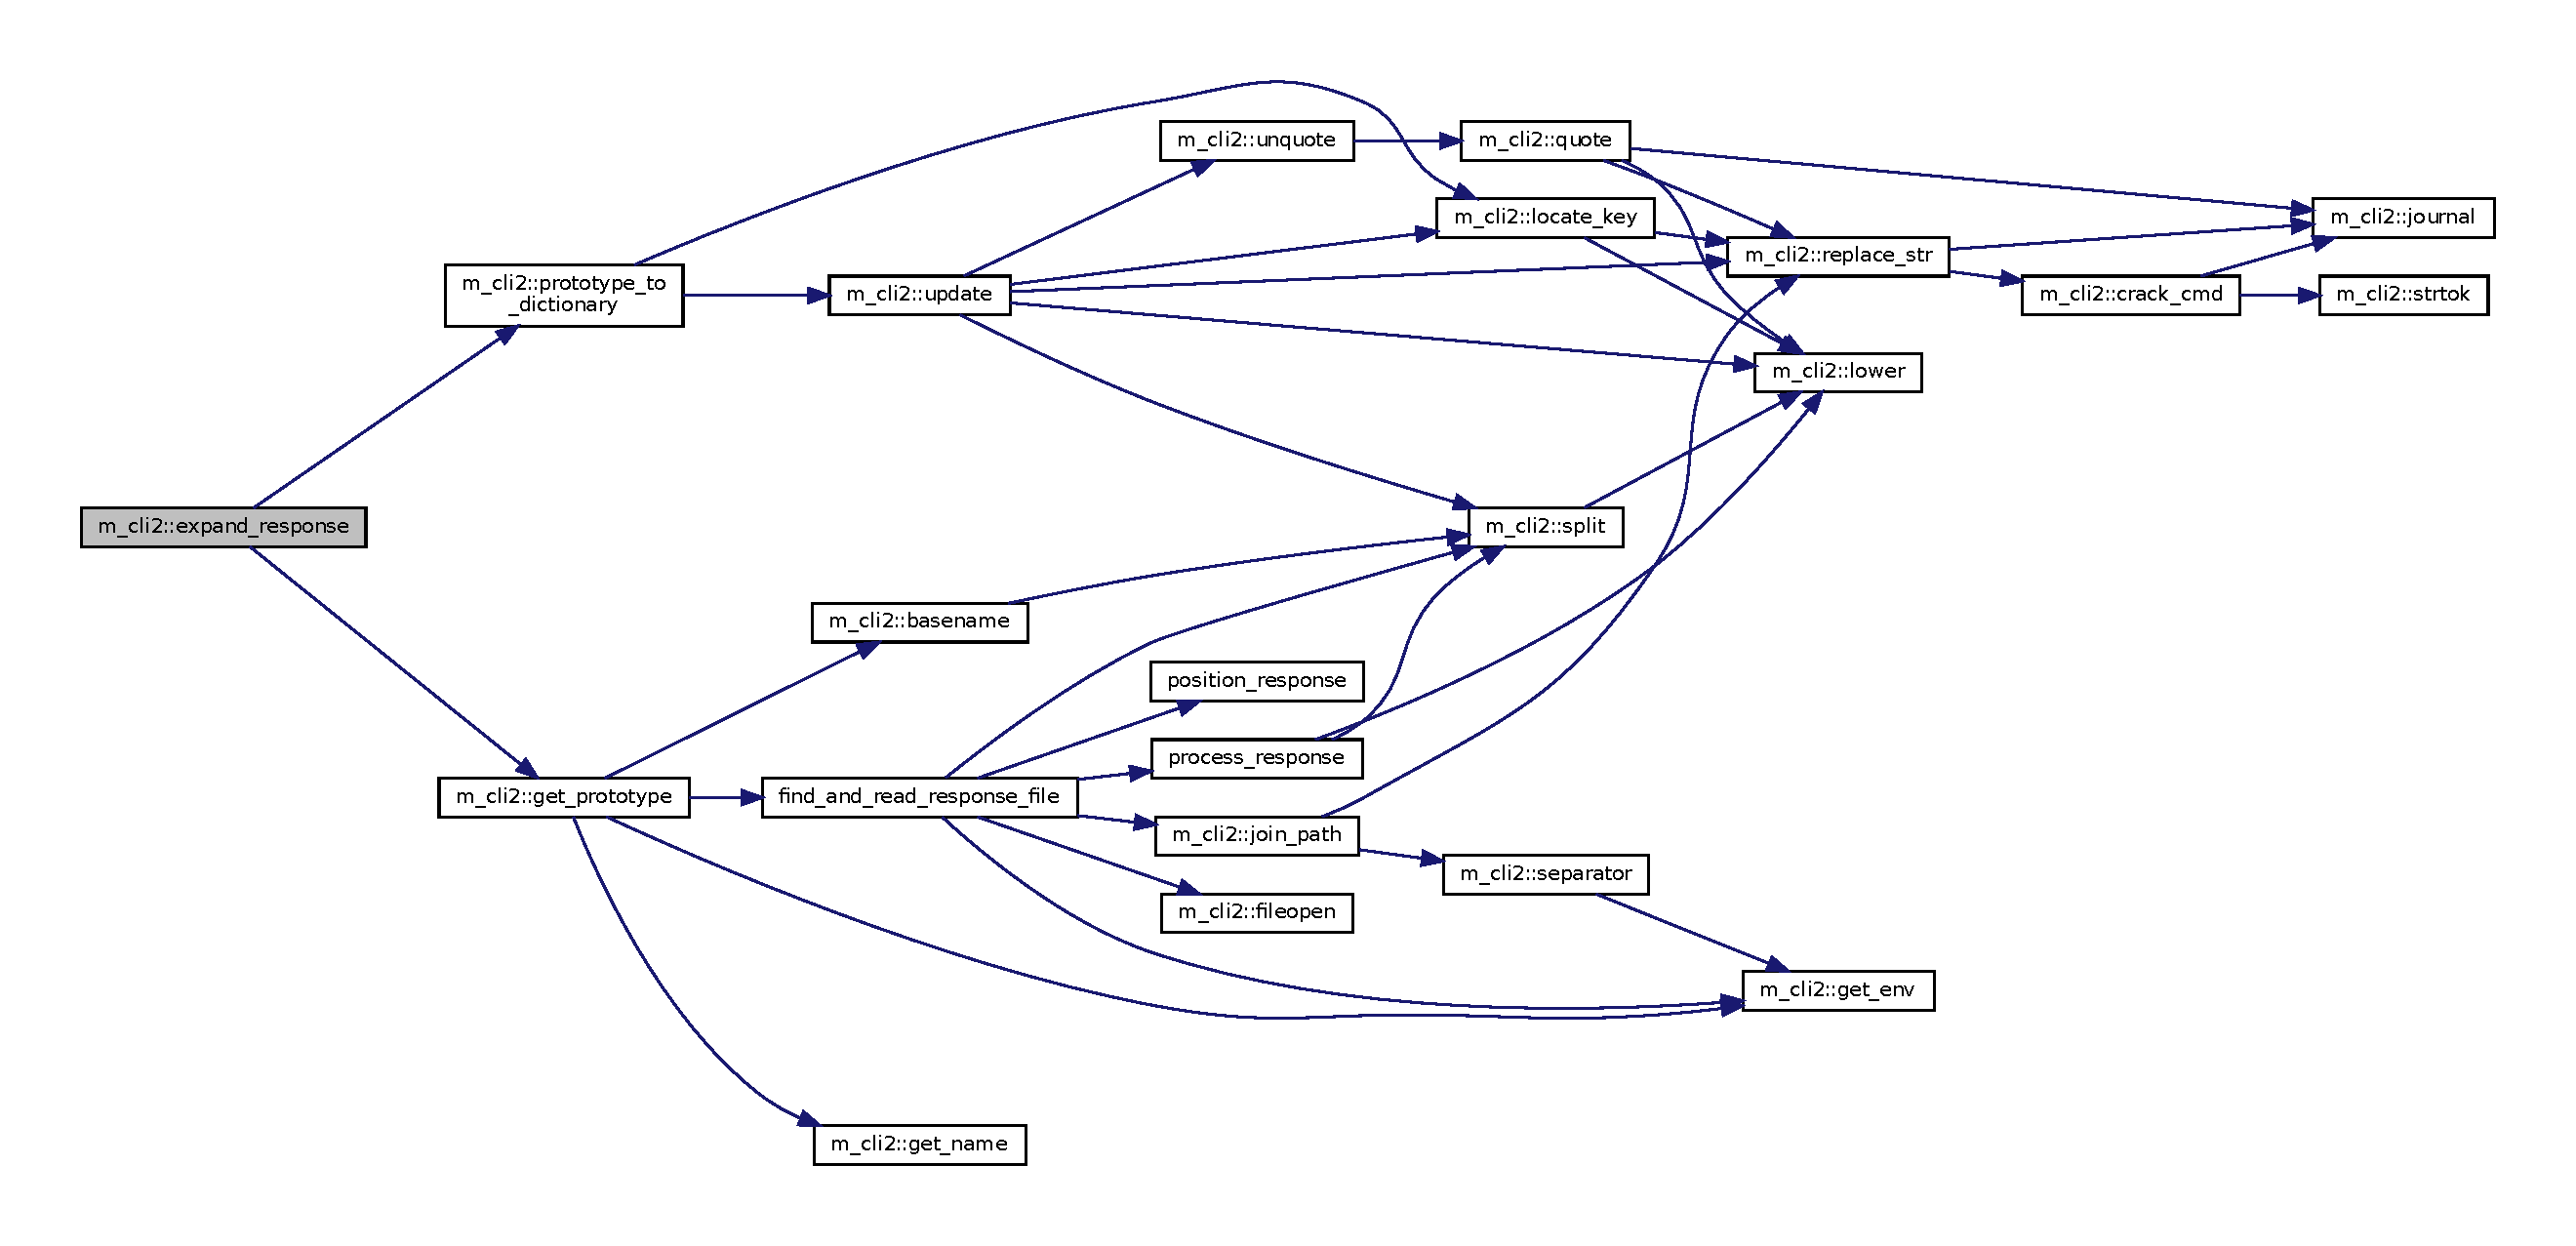
\includegraphics[width=350pt]{namespacem__cli2_a98df7b928a09462fa32a10931acf157c_cgraph}
\end{center}
\end{figure}
Here is the caller graph for this function\+:\nopagebreak
\begin{figure}[H]
\begin{center}
\leavevmode
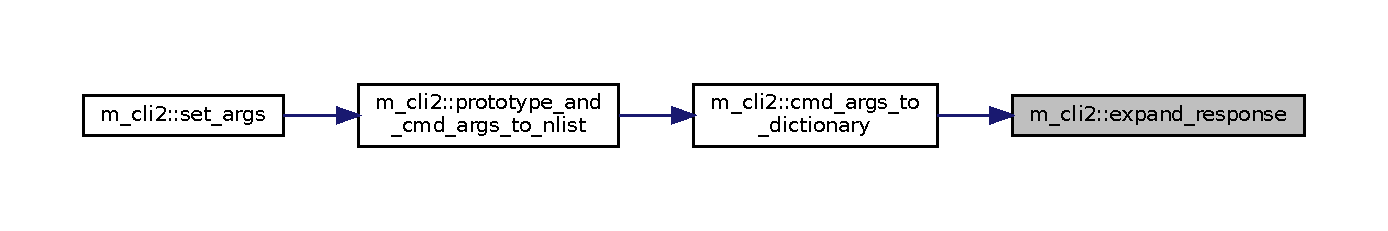
\includegraphics[width=350pt]{namespacem__cli2_a98df7b928a09462fa32a10931acf157c_icgraph}
\end{center}
\end{figure}
\mbox{\Hypertarget{namespacem__cli2_a0fadbddbbc99595fb68b333b97b89c86}\label{namespacem__cli2_a0fadbddbbc99595fb68b333b97b89c86}} 
\index{m\_cli2@{m\_cli2}!fileopen@{fileopen}}
\index{fileopen@{fileopen}!m\_cli2@{m\_cli2}}
\doxysubsubsection{\texorpdfstring{fileopen()}{fileopen()}}
{\footnotesize\ttfamily integer function m\+\_\+cli2\+::fileopen (\begin{DoxyParamCaption}\item[{character(len=$\ast$), intent(in)}]{filename,  }\item[{character(len=$\ast$), intent(out), optional}]{message }\end{DoxyParamCaption})\hspace{0.3cm}{\ttfamily [private]}}



References debug\+\_\+m\+\_\+cli2, and gen.

Here is the caller graph for this function\+:\nopagebreak
\begin{figure}[H]
\begin{center}
\leavevmode
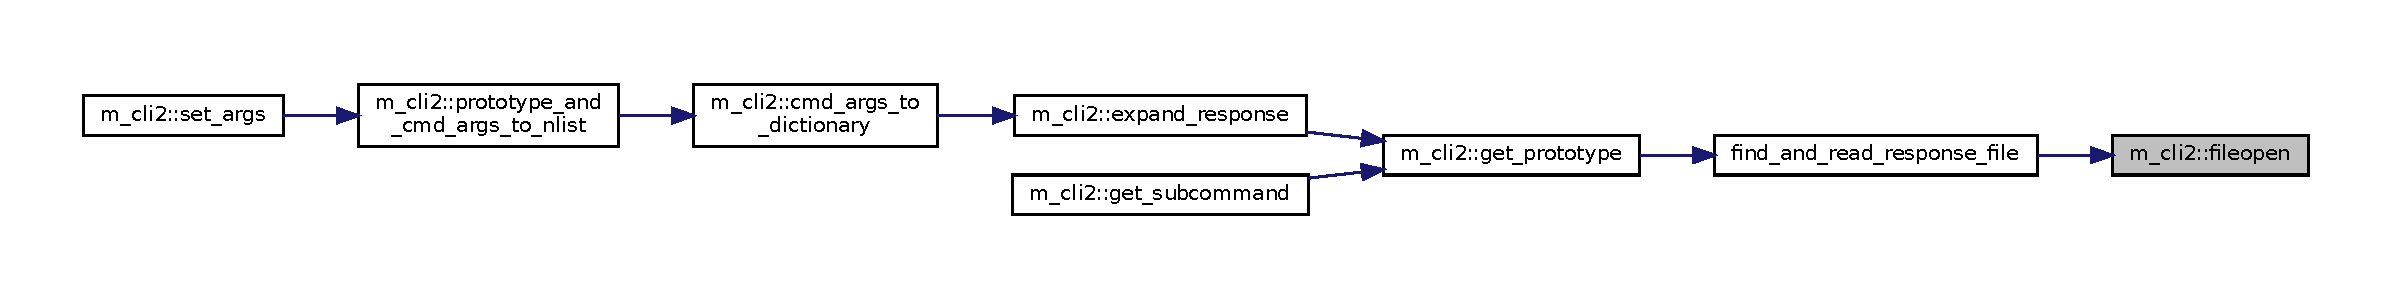
\includegraphics[width=350pt]{namespacem__cli2_a0fadbddbbc99595fb68b333b97b89c86_icgraph}
\end{center}
\end{figure}
\mbox{\Hypertarget{namespacem__cli2_aa92e8ad0300d4e324e29eae1ab9d04b4}\label{namespacem__cli2_aa92e8ad0300d4e324e29eae1ab9d04b4}} 
\index{m\_cli2@{m\_cli2}!get@{get}}
\index{get@{get}!m\_cli2@{m\_cli2}}
\doxysubsubsection{\texorpdfstring{get()}{get()}}
{\footnotesize\ttfamily character(len=\+:) function, allocatable, private m\+\_\+cli2\+::get (\begin{DoxyParamCaption}\item[{character(len=$\ast$), intent(in)}]{key }\end{DoxyParamCaption})\hspace{0.3cm}{\ttfamily [private]}}

\hypertarget{namespacem__cli2_autotoc_md62}{}\doxysubsubsection{N\+A\+ME}\label{namespacem__cli2_autotoc_md62}
get(3f) -\/ \mbox{[}A\+R\+G\+U\+M\+E\+N\+TS\+:M\+\_\+\+C\+L\+I2\mbox{]} get dictionary value associated with key name in private M\+\_\+\+C\+L\+I2(3fm) dictionary \hypertarget{namespacem__cli2_autotoc_md63}{}\doxysubsubsection{S\+Y\+N\+O\+P\+S\+IS}\label{namespacem__cli2_autotoc_md63}
\hypertarget{namespacem__cli2_autotoc_md64}{}\doxysubsubsection{D\+E\+S\+C\+R\+I\+P\+T\+I\+ON}\label{namespacem__cli2_autotoc_md64}
Get dictionary value associated with key name in private M\+\_\+\+C\+L\+I2(3fm) dictionary. \hypertarget{namespacem__cli2_autotoc_md65}{}\doxysubsubsection{O\+P\+T\+I\+O\+NS}\label{namespacem__cli2_autotoc_md65}
\hypertarget{namespacem__cli2_autotoc_md66}{}\doxysubsubsection{R\+E\+T\+U\+R\+NS}\label{namespacem__cli2_autotoc_md66}
\hypertarget{namespacem__cli2_autotoc_md67}{}\doxysubsubsection{E\+X\+A\+M\+P\+LE}\label{namespacem__cli2_autotoc_md67}


References counts, locate\+\_\+key(), and values.

Here is the call graph for this function\+:\nopagebreak
\begin{figure}[H]
\begin{center}
\leavevmode
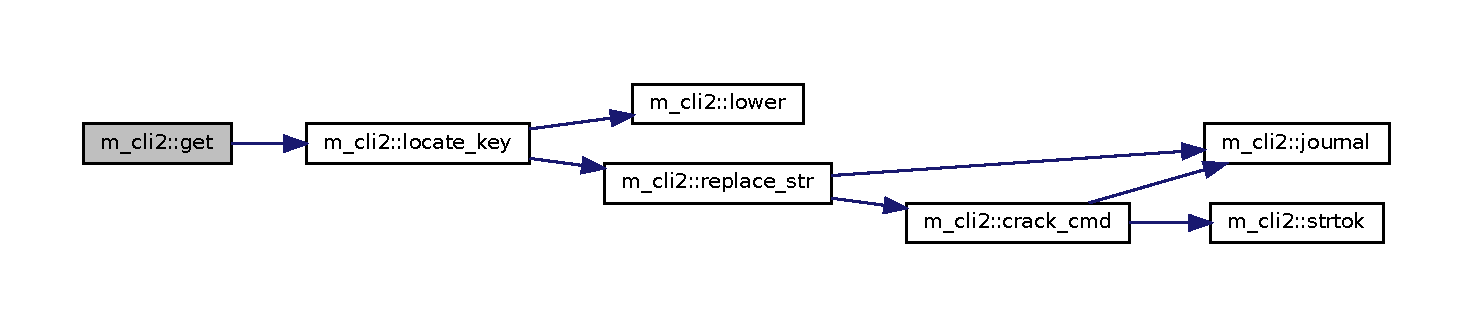
\includegraphics[width=294pt]{namespacem__cli2_aa92e8ad0300d4e324e29eae1ab9d04b4_cgraph}
\end{center}
\end{figure}
Here is the caller graph for this function\+:\nopagebreak
\begin{figure}[H]
\begin{center}
\leavevmode
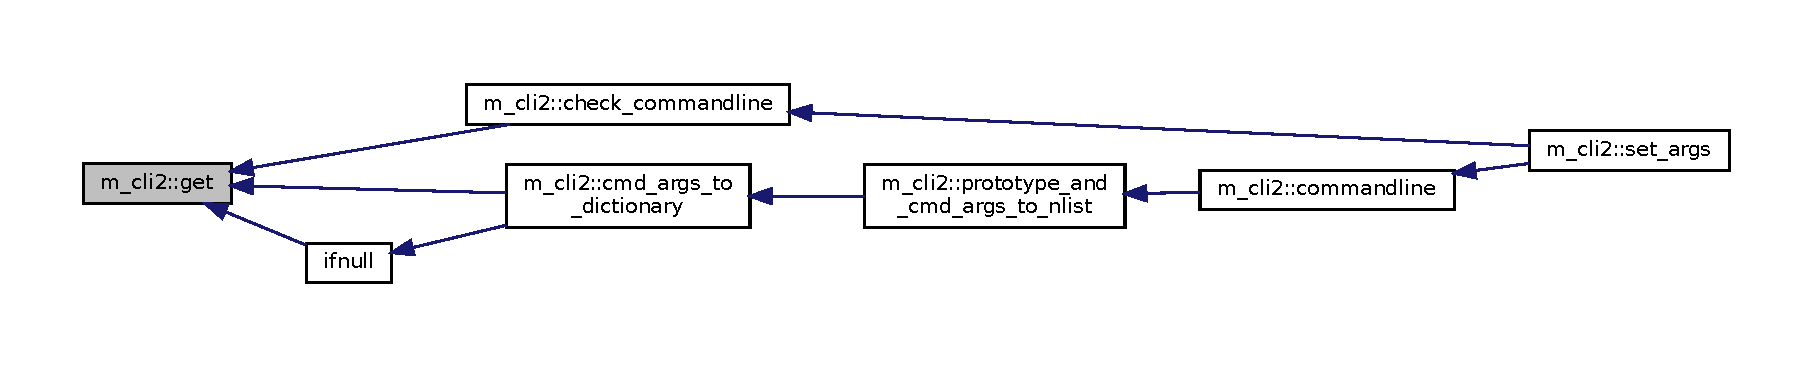
\includegraphics[width=350pt]{namespacem__cli2_aa92e8ad0300d4e324e29eae1ab9d04b4_icgraph}
\end{center}
\end{figure}
\mbox{\Hypertarget{namespacem__cli2_a448e8e24406f4bdbc14f26a940cbbc2c}\label{namespacem__cli2_a448e8e24406f4bdbc14f26a940cbbc2c}} 
\index{m\_cli2@{m\_cli2}!get\_anyarray\_c@{get\_anyarray\_c}}
\index{get\_anyarray\_c@{get\_anyarray\_c}!m\_cli2@{m\_cli2}}
\doxysubsubsection{\texorpdfstring{get\_anyarray\_c()}{get\_anyarray\_c()}}
{\footnotesize\ttfamily subroutine m\+\_\+cli2\+::get\+\_\+anyarray\+\_\+c (\begin{DoxyParamCaption}\item[{character(len=$\ast$), intent(in)}]{keyword,  }\item[{character(len=\+:), dimension(\+:), allocatable}]{strings,  }\item[{character(len=$\ast$), intent(in), optional}]{delimiters }\end{DoxyParamCaption})\hspace{0.3cm}{\ttfamily [private]}}



References counts, journal(), locate\+\_\+key(), mystop(), split(), unquote(), and values.

Here is the call graph for this function\+:\nopagebreak
\begin{figure}[H]
\begin{center}
\leavevmode
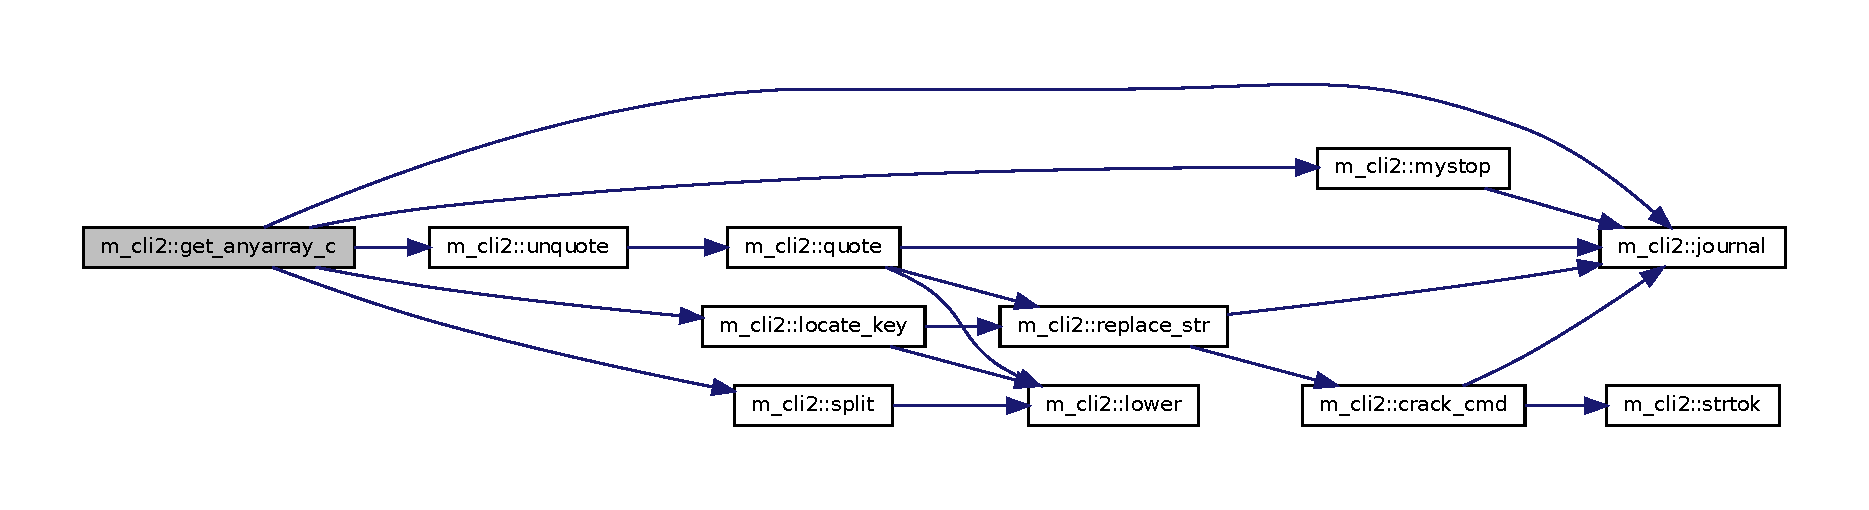
\includegraphics[width=350pt]{namespacem__cli2_a448e8e24406f4bdbc14f26a940cbbc2c_cgraph}
\end{center}
\end{figure}
\mbox{\Hypertarget{namespacem__cli2_aaede1f28172778cf45f4b6c04967bbbd}\label{namespacem__cli2_aaede1f28172778cf45f4b6c04967bbbd}} 
\index{m\_cli2@{m\_cli2}!get\_anyarray\_d@{get\_anyarray\_d}}
\index{get\_anyarray\_d@{get\_anyarray\_d}!m\_cli2@{m\_cli2}}
\doxysubsubsection{\texorpdfstring{get\_anyarray\_d()}{get\_anyarray\_d()}}
{\footnotesize\ttfamily subroutine m\+\_\+cli2\+::get\+\_\+anyarray\+\_\+d (\begin{DoxyParamCaption}\item[{character(len=$\ast$), intent(in)}]{keyword,  }\item[{real(kind=\mbox{\hyperlink{namespacem__cli2_acf83f1963cf6a56ad0221cfcf5402440}{dp}}), dimension(\+:), intent(out), allocatable}]{darray,  }\item[{character(len=$\ast$), intent(in), optional}]{delimiters }\end{DoxyParamCaption})\hspace{0.3cm}{\ttfamily [private]}}



References a2d(), counts, journal(), locate\+\_\+key(), mystop(), replace\+\_\+str(), split(), and values.

Here is the call graph for this function\+:\nopagebreak
\begin{figure}[H]
\begin{center}
\leavevmode
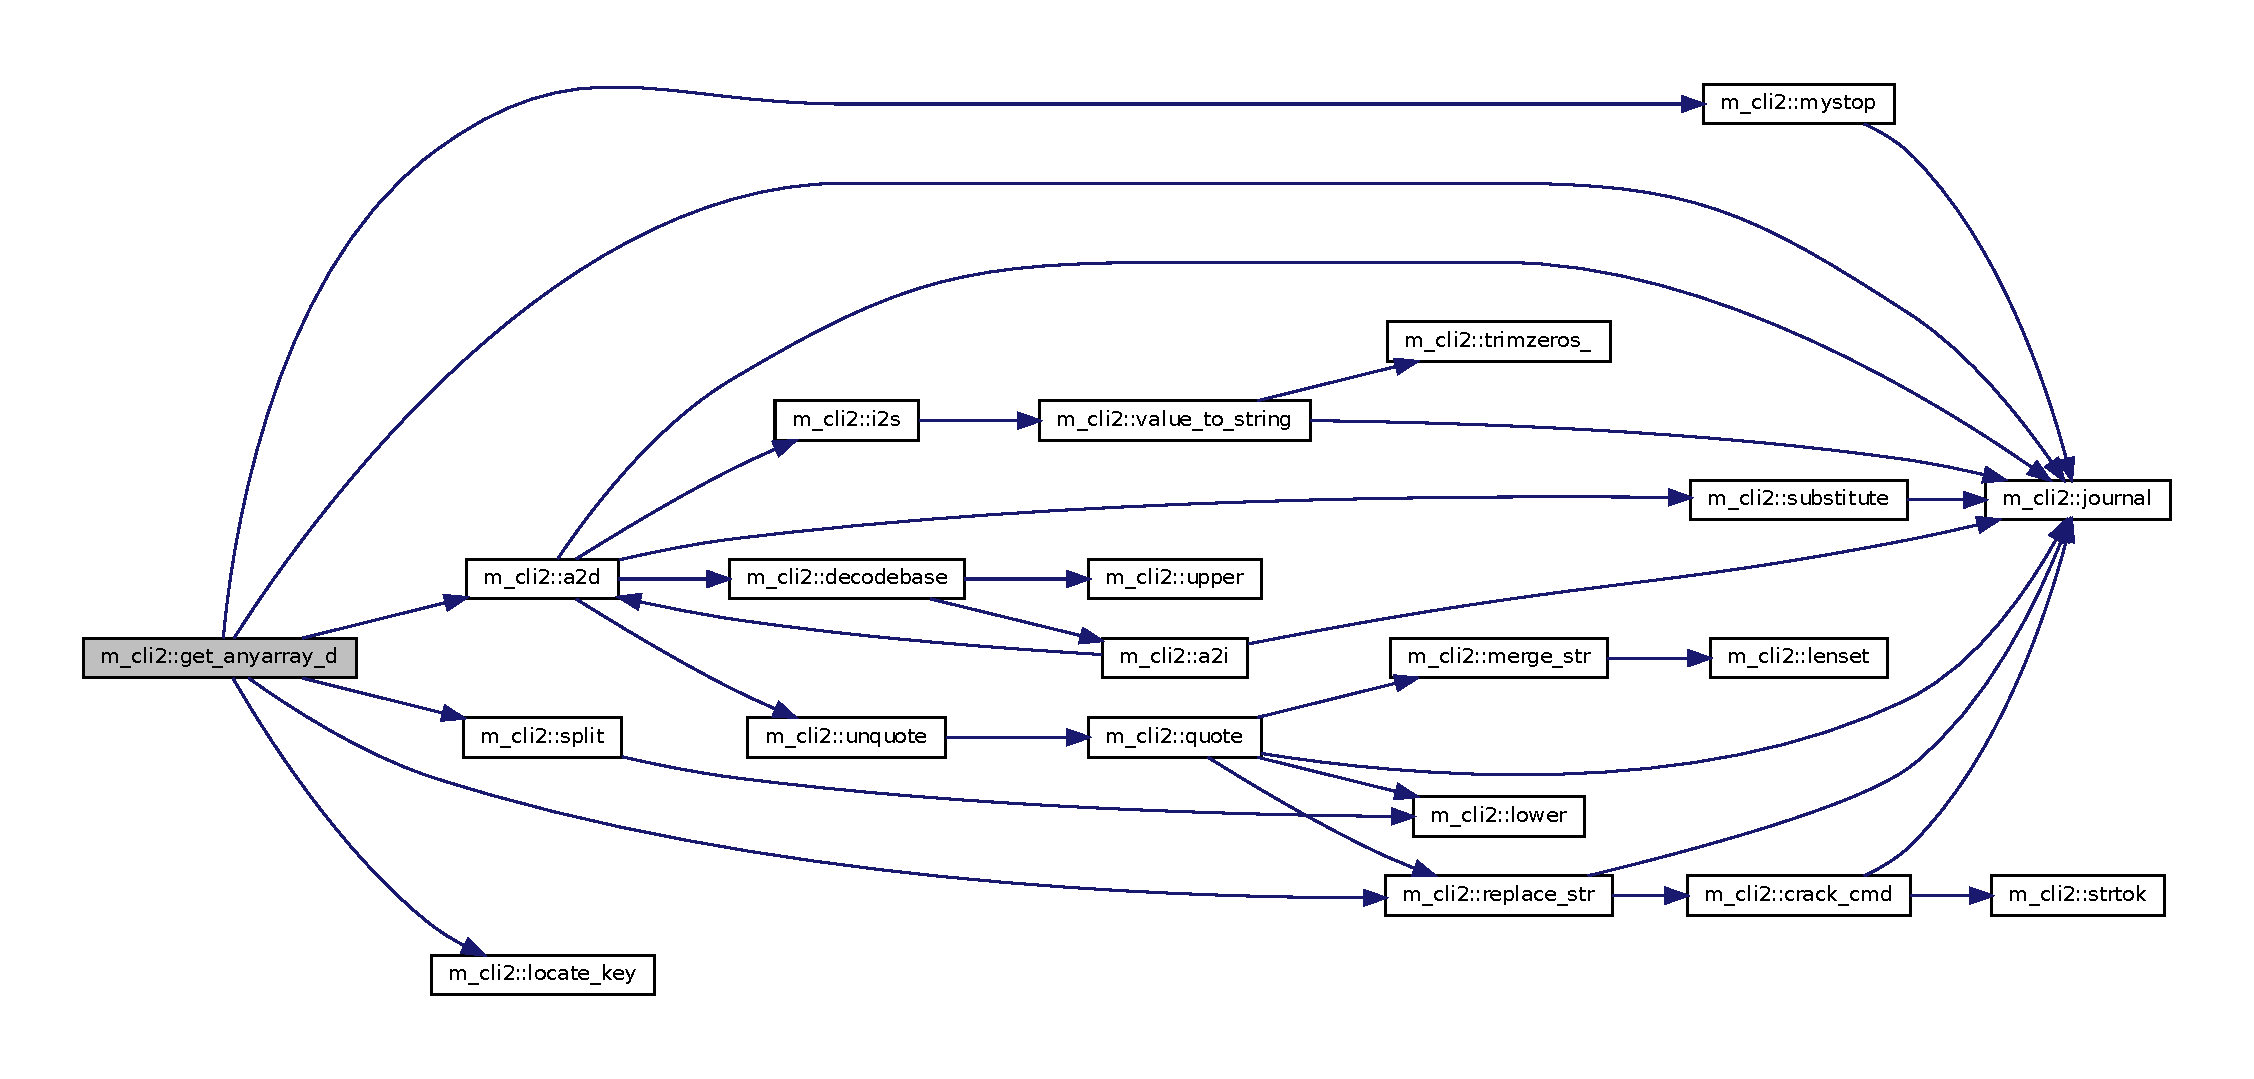
\includegraphics[width=350pt]{namespacem__cli2_aaede1f28172778cf45f4b6c04967bbbd_cgraph}
\end{center}
\end{figure}
Here is the caller graph for this function\+:\nopagebreak
\begin{figure}[H]
\begin{center}
\leavevmode
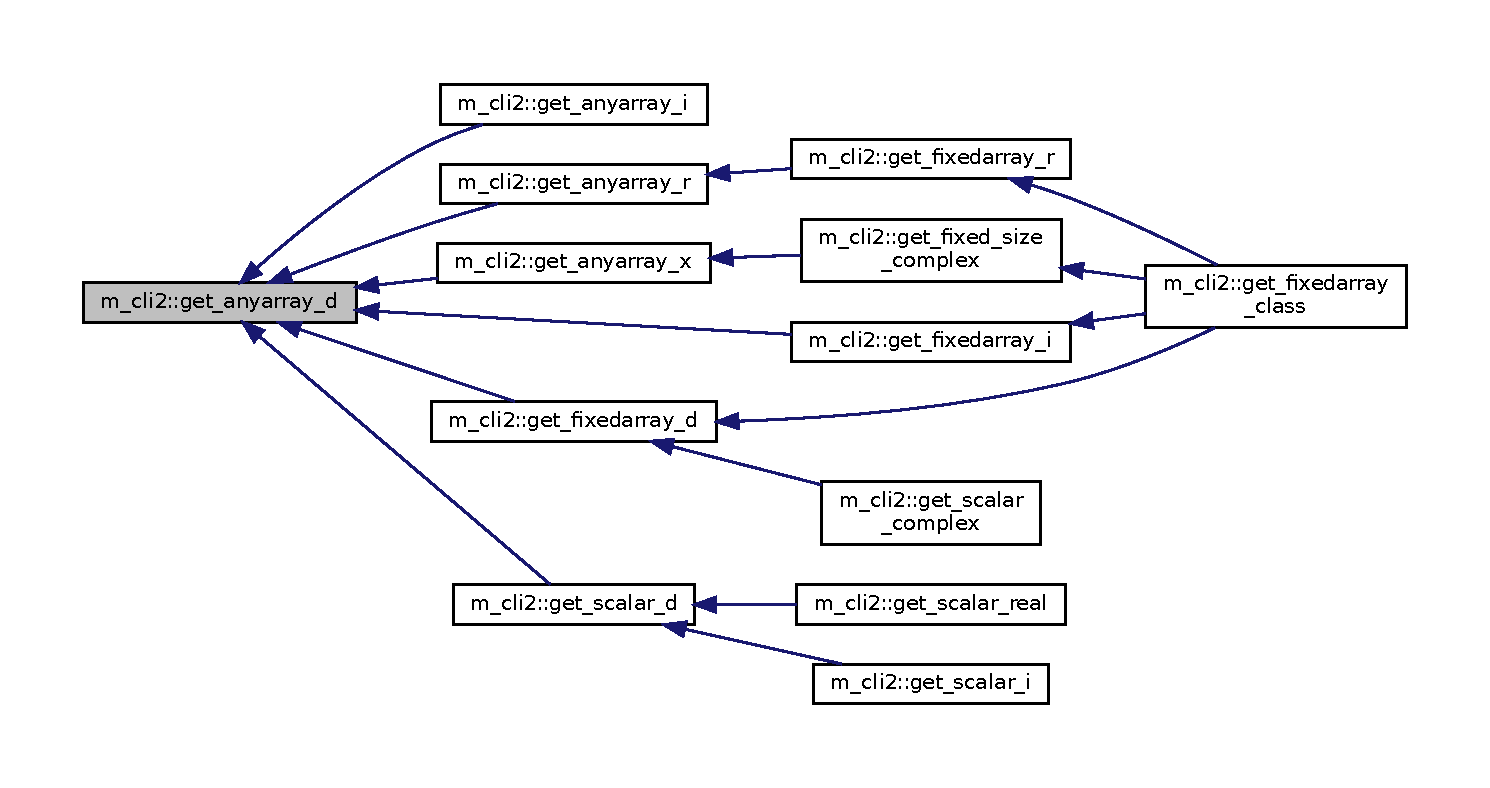
\includegraphics[width=350pt]{namespacem__cli2_aaede1f28172778cf45f4b6c04967bbbd_icgraph}
\end{center}
\end{figure}
\mbox{\Hypertarget{namespacem__cli2_ad314315dd5c93abff5168265f5ff0e4e}\label{namespacem__cli2_ad314315dd5c93abff5168265f5ff0e4e}} 
\index{m\_cli2@{m\_cli2}!get\_anyarray\_i@{get\_anyarray\_i}}
\index{get\_anyarray\_i@{get\_anyarray\_i}!m\_cli2@{m\_cli2}}
\doxysubsubsection{\texorpdfstring{get\_anyarray\_i()}{get\_anyarray\_i()}}
{\footnotesize\ttfamily subroutine m\+\_\+cli2\+::get\+\_\+anyarray\+\_\+i (\begin{DoxyParamCaption}\item[{character(len=$\ast$), intent(in)}]{keyword,  }\item[{integer, dimension(\+:), allocatable}]{iarray,  }\item[{character(len=$\ast$), intent(in), optional}]{delimiters }\end{DoxyParamCaption})\hspace{0.3cm}{\ttfamily [private]}}



References get\+\_\+anyarray\+\_\+d().

Here is the call graph for this function\+:\nopagebreak
\begin{figure}[H]
\begin{center}
\leavevmode
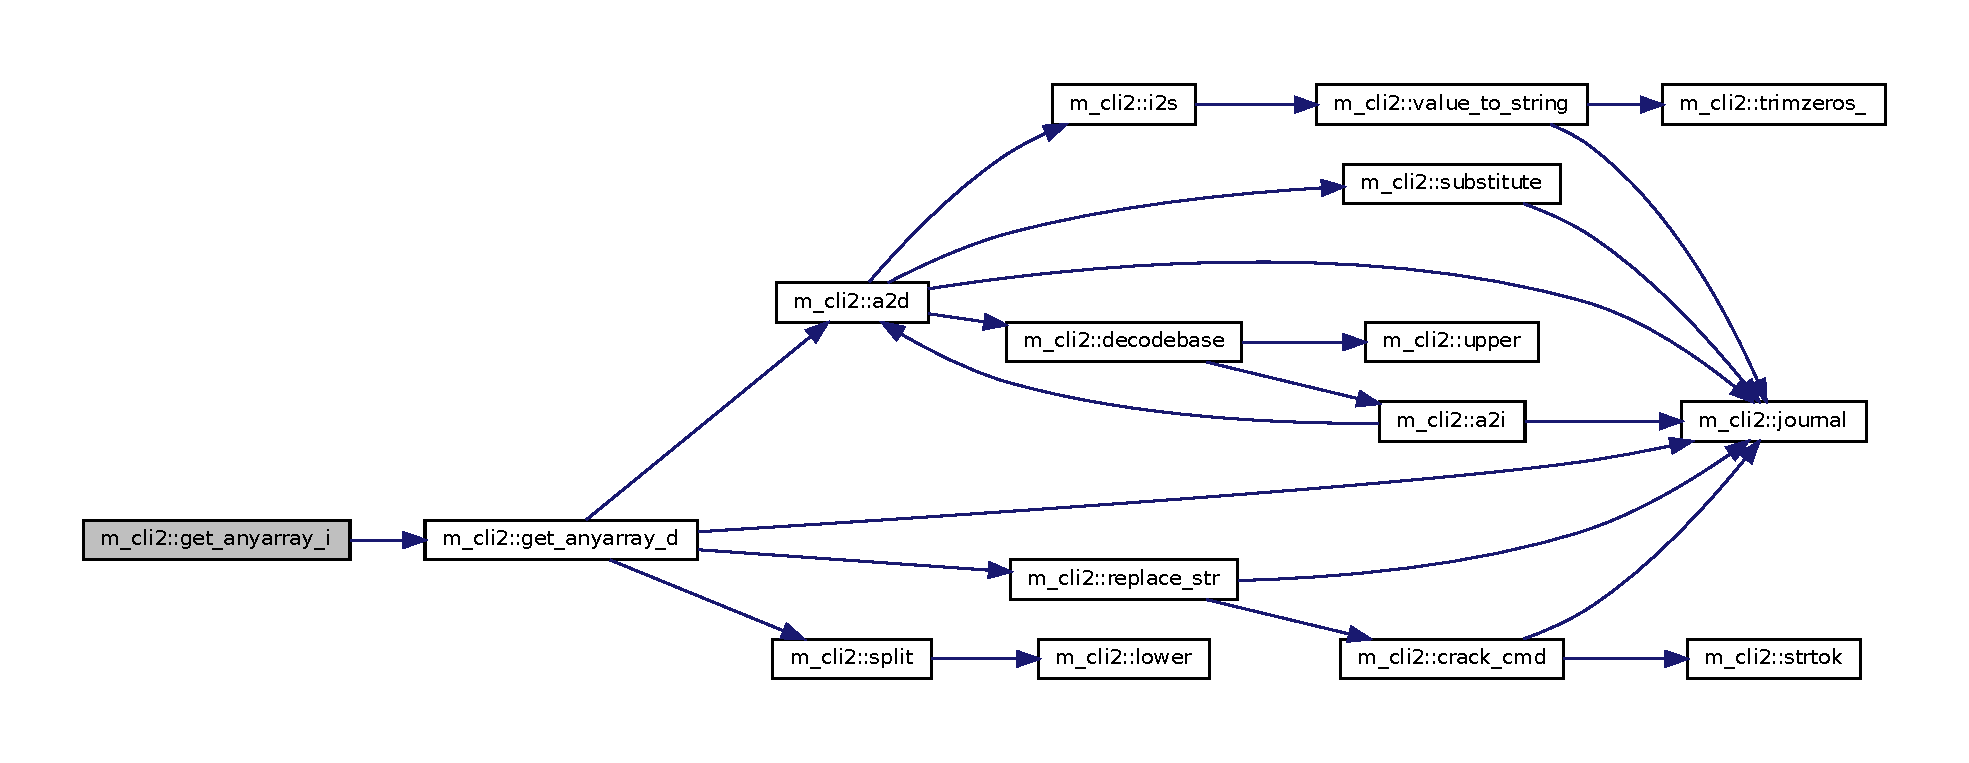
\includegraphics[width=350pt]{namespacem__cli2_ad314315dd5c93abff5168265f5ff0e4e_cgraph}
\end{center}
\end{figure}
\mbox{\Hypertarget{namespacem__cli2_a47cc758d20b655bc21672c31289e54ce}\label{namespacem__cli2_a47cc758d20b655bc21672c31289e54ce}} 
\index{m\_cli2@{m\_cli2}!get\_anyarray\_l@{get\_anyarray\_l}}
\index{get\_anyarray\_l@{get\_anyarray\_l}!m\_cli2@{m\_cli2}}
\doxysubsubsection{\texorpdfstring{get\_anyarray\_l()}{get\_anyarray\_l()}}
{\footnotesize\ttfamily subroutine m\+\_\+cli2\+::get\+\_\+anyarray\+\_\+l (\begin{DoxyParamCaption}\item[{character(len=$\ast$), intent(in)}]{keyword,  }\item[{logical, dimension(\+:), allocatable}]{larray,  }\item[{character(len=$\ast$), intent(in), optional}]{delimiters }\end{DoxyParamCaption})\hspace{0.3cm}{\ttfamily [private]}}



References counts, journal(), locate\+\_\+key(), mystop(), split(), upper(), and values.

Here is the call graph for this function\+:\nopagebreak
\begin{figure}[H]
\begin{center}
\leavevmode
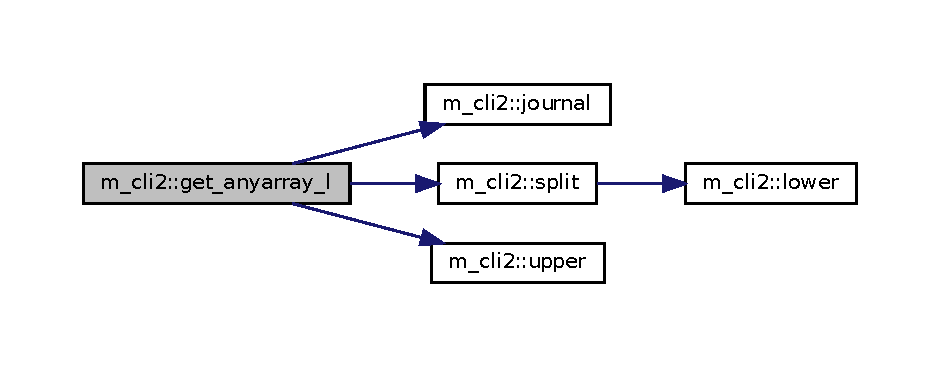
\includegraphics[width=350pt]{namespacem__cli2_a47cc758d20b655bc21672c31289e54ce_cgraph}
\end{center}
\end{figure}
Here is the caller graph for this function\+:\nopagebreak
\begin{figure}[H]
\begin{center}
\leavevmode
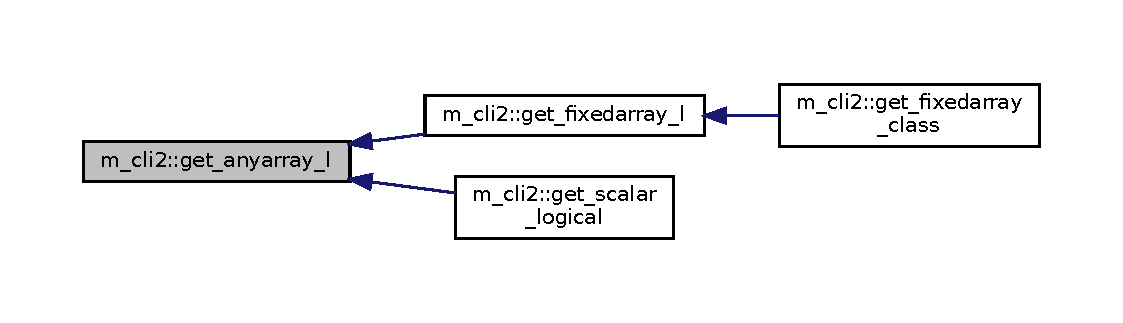
\includegraphics[width=350pt]{namespacem__cli2_a47cc758d20b655bc21672c31289e54ce_icgraph}
\end{center}
\end{figure}
\mbox{\Hypertarget{namespacem__cli2_a8f1d5223b075f23d513c94548a1ebf09}\label{namespacem__cli2_a8f1d5223b075f23d513c94548a1ebf09}} 
\index{m\_cli2@{m\_cli2}!get\_anyarray\_r@{get\_anyarray\_r}}
\index{get\_anyarray\_r@{get\_anyarray\_r}!m\_cli2@{m\_cli2}}
\doxysubsubsection{\texorpdfstring{get\_anyarray\_r()}{get\_anyarray\_r()}}
{\footnotesize\ttfamily subroutine m\+\_\+cli2\+::get\+\_\+anyarray\+\_\+r (\begin{DoxyParamCaption}\item[{character(len=$\ast$), intent(in)}]{keyword,  }\item[{real, dimension(\+:), allocatable}]{rarray,  }\item[{character(len=$\ast$), intent(in), optional}]{delimiters }\end{DoxyParamCaption})\hspace{0.3cm}{\ttfamily [private]}}



References get\+\_\+anyarray\+\_\+d().

Here is the call graph for this function\+:\nopagebreak
\begin{figure}[H]
\begin{center}
\leavevmode
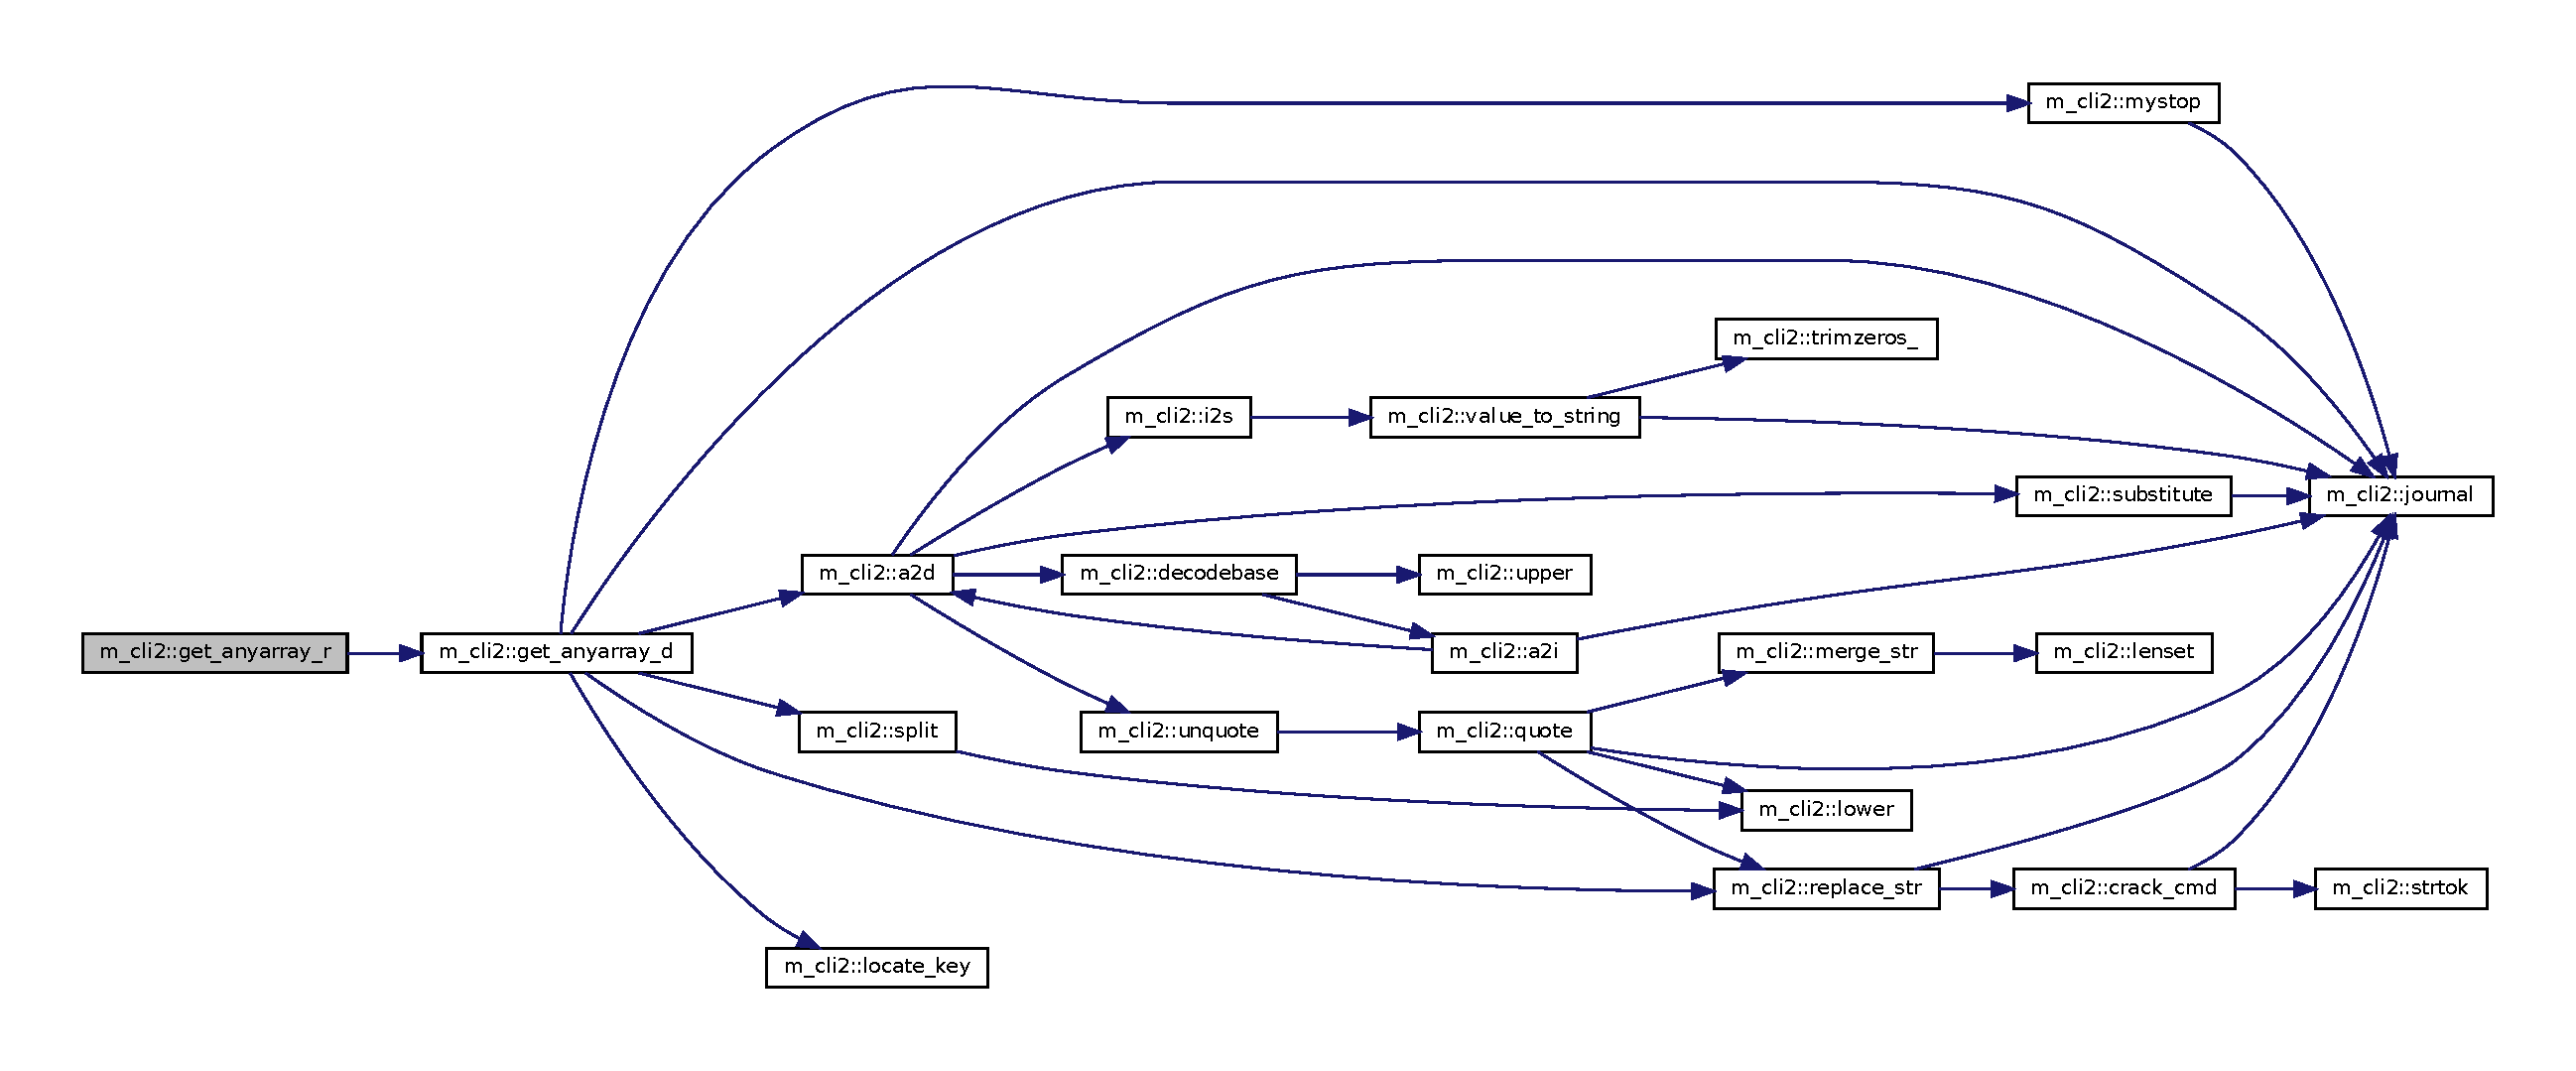
\includegraphics[width=350pt]{namespacem__cli2_a8f1d5223b075f23d513c94548a1ebf09_cgraph}
\end{center}
\end{figure}
Here is the caller graph for this function\+:\nopagebreak
\begin{figure}[H]
\begin{center}
\leavevmode
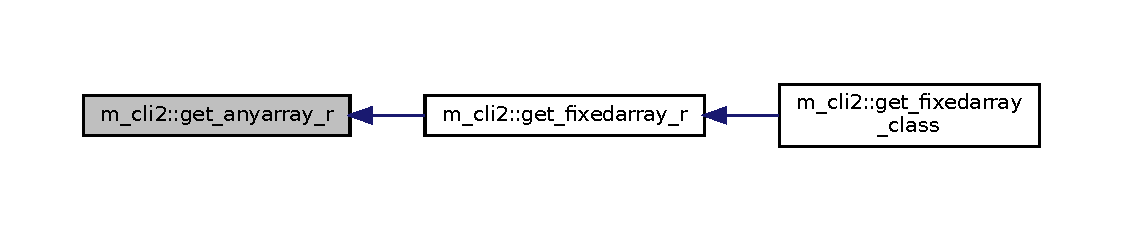
\includegraphics[width=350pt]{namespacem__cli2_a8f1d5223b075f23d513c94548a1ebf09_icgraph}
\end{center}
\end{figure}
\mbox{\Hypertarget{namespacem__cli2_ab9ab288fa5f108beeb7c94d81b223b7c}\label{namespacem__cli2_ab9ab288fa5f108beeb7c94d81b223b7c}} 
\index{m\_cli2@{m\_cli2}!get\_anyarray\_x@{get\_anyarray\_x}}
\index{get\_anyarray\_x@{get\_anyarray\_x}!m\_cli2@{m\_cli2}}
\doxysubsubsection{\texorpdfstring{get\_anyarray\_x()}{get\_anyarray\_x()}}
{\footnotesize\ttfamily subroutine m\+\_\+cli2\+::get\+\_\+anyarray\+\_\+x (\begin{DoxyParamCaption}\item[{character(len=$\ast$), intent(in)}]{keyword,  }\item[{complex, dimension(\+:), allocatable}]{xarray,  }\item[{character(len=$\ast$), intent(in), optional}]{delimiters }\end{DoxyParamCaption})\hspace{0.3cm}{\ttfamily [private]}}



References get\+\_\+anyarray\+\_\+d(), journal(), and mystop().

Here is the call graph for this function\+:\nopagebreak
\begin{figure}[H]
\begin{center}
\leavevmode
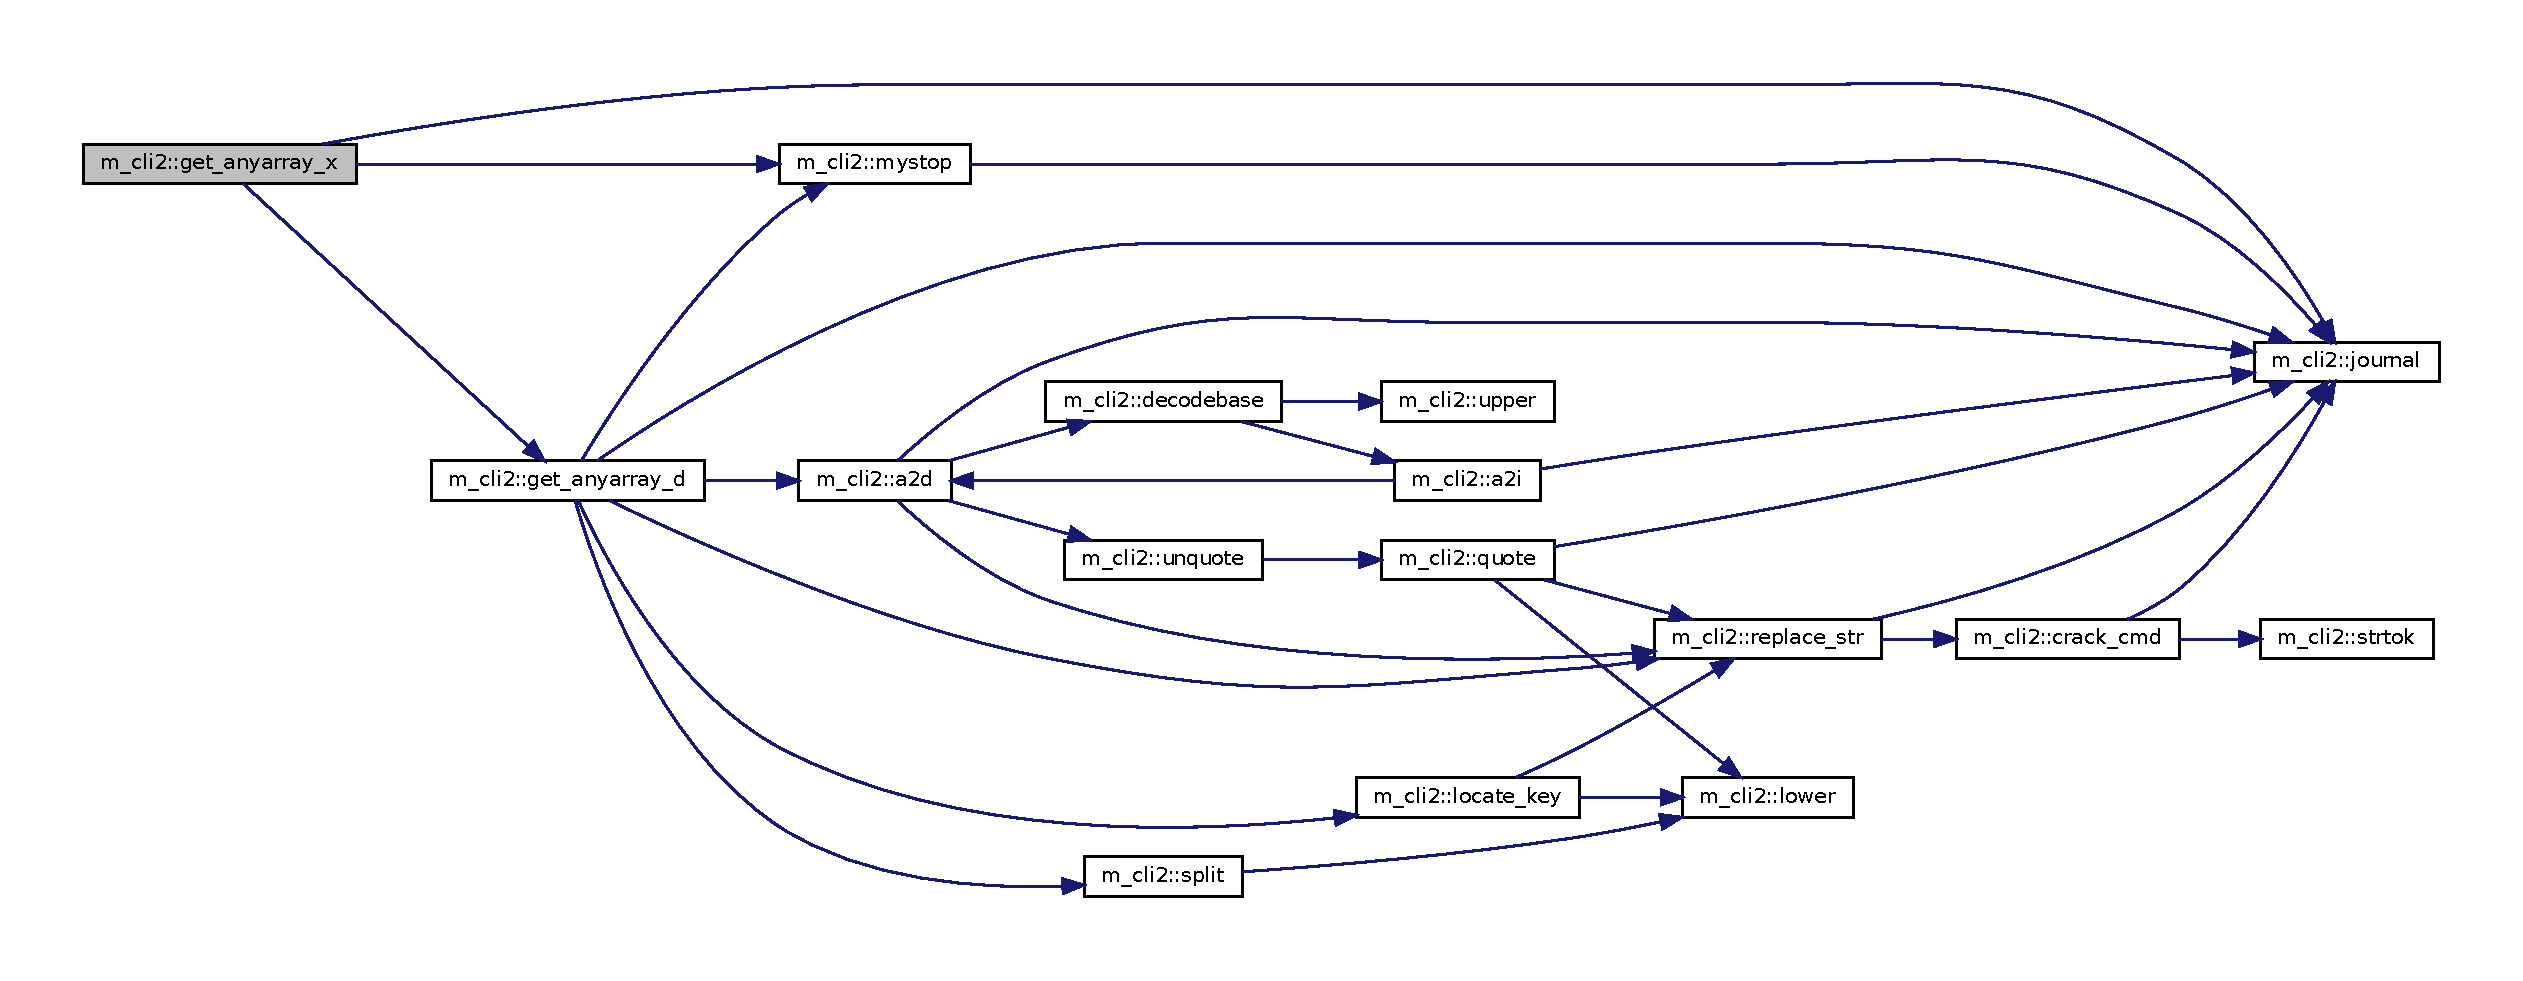
\includegraphics[width=350pt]{namespacem__cli2_ab9ab288fa5f108beeb7c94d81b223b7c_cgraph}
\end{center}
\end{figure}
Here is the caller graph for this function\+:\nopagebreak
\begin{figure}[H]
\begin{center}
\leavevmode
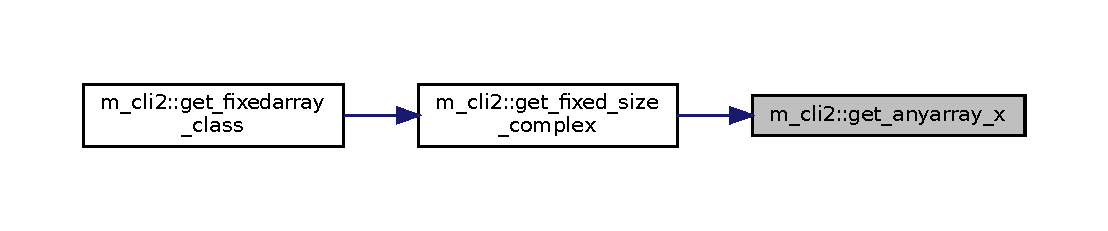
\includegraphics[width=350pt]{namespacem__cli2_ab9ab288fa5f108beeb7c94d81b223b7c_icgraph}
\end{center}
\end{figure}
\mbox{\Hypertarget{namespacem__cli2_ae5de7b1fadd37dab33579de6de349fd0}\label{namespacem__cli2_ae5de7b1fadd37dab33579de6de349fd0}} 
\index{m\_cli2@{m\_cli2}!get\_args\_fixed\_length\_a\_array@{get\_args\_fixed\_length\_a\_array}}
\index{get\_args\_fixed\_length\_a\_array@{get\_args\_fixed\_length\_a\_array}!m\_cli2@{m\_cli2}}
\doxysubsubsection{\texorpdfstring{get\_args\_fixed\_length\_a\_array()}{get\_args\_fixed\_length\_a\_array()}}
{\footnotesize\ttfamily subroutine m\+\_\+cli2\+::get\+\_\+args\+\_\+fixed\+\_\+length\+\_\+a\+\_\+array (\begin{DoxyParamCaption}\item[{character(len=$\ast$), intent(in)}]{keyword,  }\item[{character(len=$\ast$), dimension(\+:), allocatable}]{strings,  }\item[{character(len=$\ast$), intent(in), optional}]{delimiters }\end{DoxyParamCaption})\hspace{0.3cm}{\ttfamily [private]}}



References counts, journal(), locate\+\_\+key(), mystop(), split(), unquote(), and values.

Here is the call graph for this function\+:\nopagebreak
\begin{figure}[H]
\begin{center}
\leavevmode
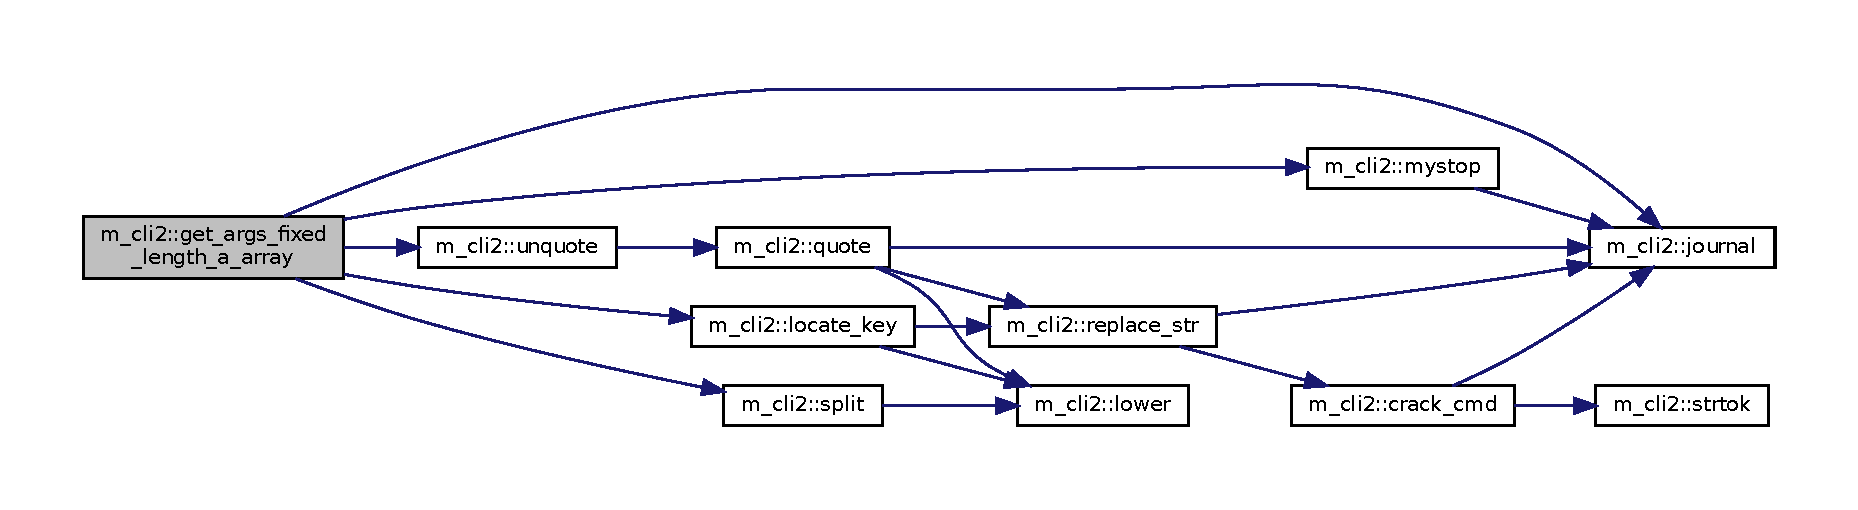
\includegraphics[width=350pt]{namespacem__cli2_ae5de7b1fadd37dab33579de6de349fd0_cgraph}
\end{center}
\end{figure}
\mbox{\Hypertarget{namespacem__cli2_a2762ef1e3ed8710a7068d338f61c3da3}\label{namespacem__cli2_a2762ef1e3ed8710a7068d338f61c3da3}} 
\index{m\_cli2@{m\_cli2}!get\_args\_fixed\_length\_scalar\_c@{get\_args\_fixed\_length\_scalar\_c}}
\index{get\_args\_fixed\_length\_scalar\_c@{get\_args\_fixed\_length\_scalar\_c}!m\_cli2@{m\_cli2}}
\doxysubsubsection{\texorpdfstring{get\_args\_fixed\_length\_scalar\_c()}{get\_args\_fixed\_length\_scalar\_c()}}
{\footnotesize\ttfamily elemental impure subroutine m\+\_\+cli2\+::get\+\_\+args\+\_\+fixed\+\_\+length\+\_\+scalar\+\_\+c (\begin{DoxyParamCaption}\item[{character(len=$\ast$), intent(in)}]{keyword,  }\item[{character(len=$\ast$), intent(out)}]{string }\end{DoxyParamCaption})\hspace{0.3cm}{\ttfamily [private]}}



References counts, journal(), locate\+\_\+key(), mystop(), unquote(), and values.

Here is the call graph for this function\+:\nopagebreak
\begin{figure}[H]
\begin{center}
\leavevmode
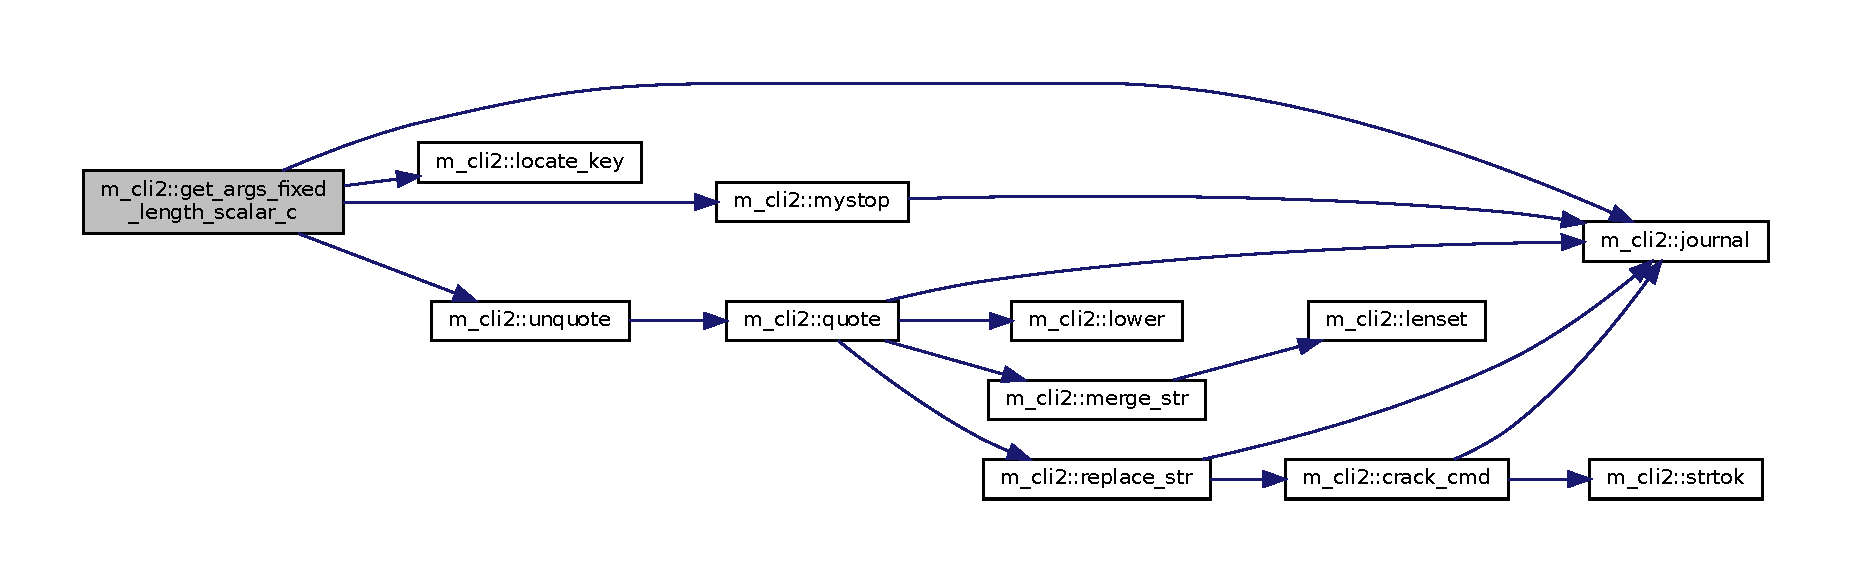
\includegraphics[width=350pt]{namespacem__cli2_a2762ef1e3ed8710a7068d338f61c3da3_cgraph}
\end{center}
\end{figure}
\mbox{\Hypertarget{namespacem__cli2_a1a3a7cb7ef271b1cfce52525860ac9d7}\label{namespacem__cli2_a1a3a7cb7ef271b1cfce52525860ac9d7}} 
\index{m\_cli2@{m\_cli2}!get\_env@{get\_env}}
\index{get\_env@{get\_env}!m\_cli2@{m\_cli2}}
\doxysubsubsection{\texorpdfstring{get\_env()}{get\_env()}}
{\footnotesize\ttfamily character(len=\+:) function, allocatable m\+\_\+cli2\+::get\+\_\+env (\begin{DoxyParamCaption}\item[{character(len=$\ast$), intent(in)}]{N\+A\+ME,  }\item[{character(len=$\ast$), intent(in), optional}]{D\+E\+F\+A\+U\+LT }\end{DoxyParamCaption})\hspace{0.3cm}{\ttfamily [private]}}

Here is the caller graph for this function\+:\nopagebreak
\begin{figure}[H]
\begin{center}
\leavevmode
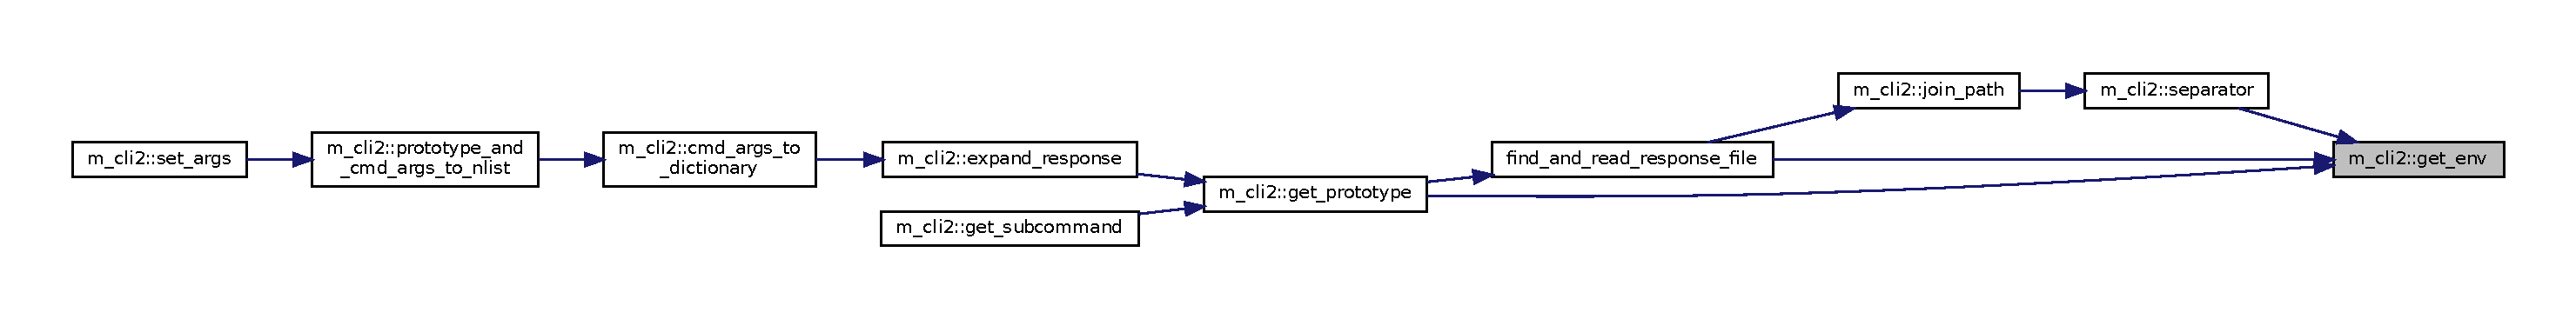
\includegraphics[width=350pt]{namespacem__cli2_a1a3a7cb7ef271b1cfce52525860ac9d7_icgraph}
\end{center}
\end{figure}
\mbox{\Hypertarget{namespacem__cli2_a32b78784e20e29bf40f17e16d08336fa}\label{namespacem__cli2_a32b78784e20e29bf40f17e16d08336fa}} 
\index{m\_cli2@{m\_cli2}!get\_fixed\_size\_complex@{get\_fixed\_size\_complex}}
\index{get\_fixed\_size\_complex@{get\_fixed\_size\_complex}!m\_cli2@{m\_cli2}}
\doxysubsubsection{\texorpdfstring{get\_fixed\_size\_complex()}{get\_fixed\_size\_complex()}}
{\footnotesize\ttfamily subroutine m\+\_\+cli2\+::get\+\_\+fixed\+\_\+size\+\_\+complex (\begin{DoxyParamCaption}\item[{character(len=$\ast$), intent(in)}]{keyword,  }\item[{complex, dimension(\+:)}]{xarray,  }\item[{character(len=$\ast$), intent(in), optional}]{delimiters }\end{DoxyParamCaption})\hspace{0.3cm}{\ttfamily [private]}}



References get\+\_\+anyarray\+\_\+x(), journal(), mystop(), and print\+\_\+dictionary().

Here is the call graph for this function\+:\nopagebreak
\begin{figure}[H]
\begin{center}
\leavevmode
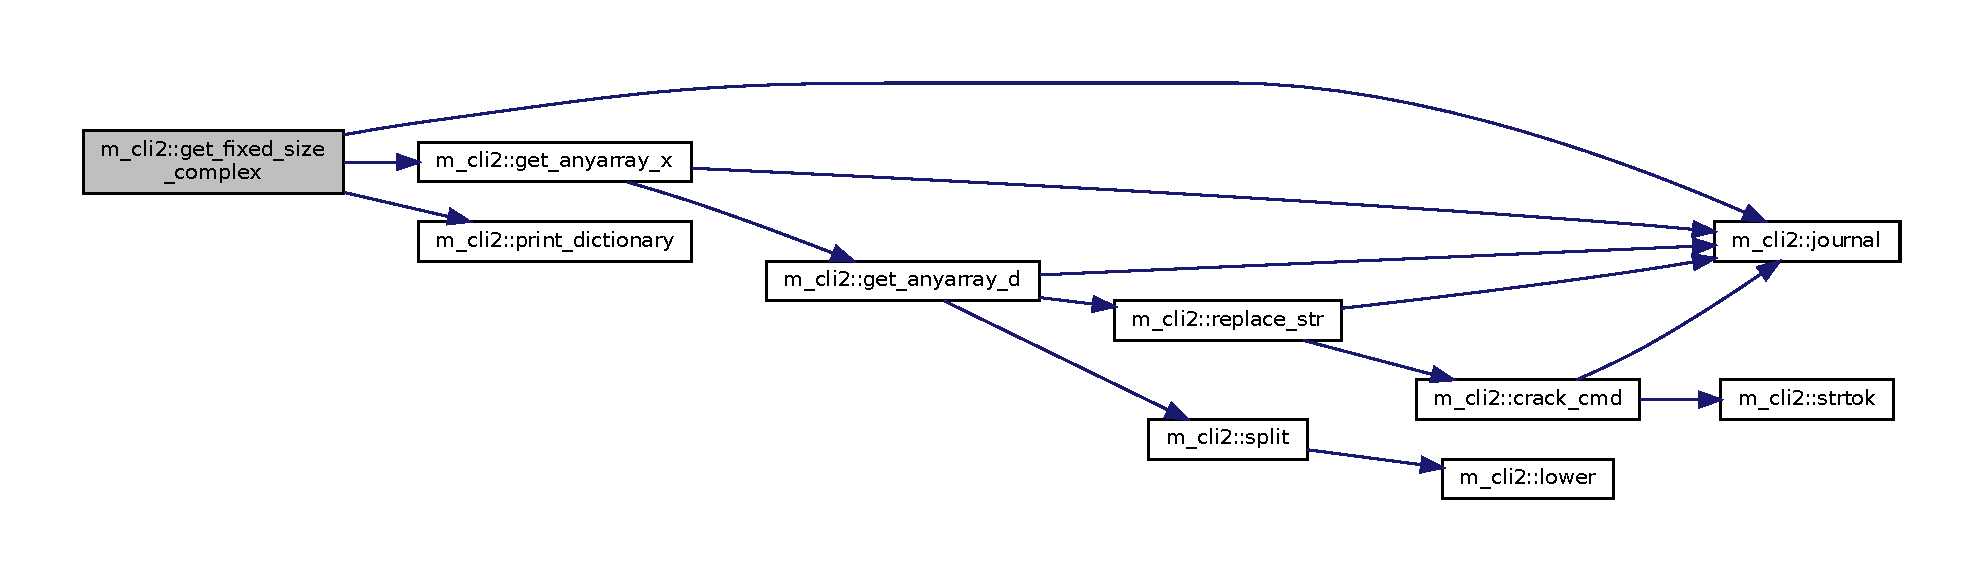
\includegraphics[width=350pt]{namespacem__cli2_a32b78784e20e29bf40f17e16d08336fa_cgraph}
\end{center}
\end{figure}
Here is the caller graph for this function\+:\nopagebreak
\begin{figure}[H]
\begin{center}
\leavevmode
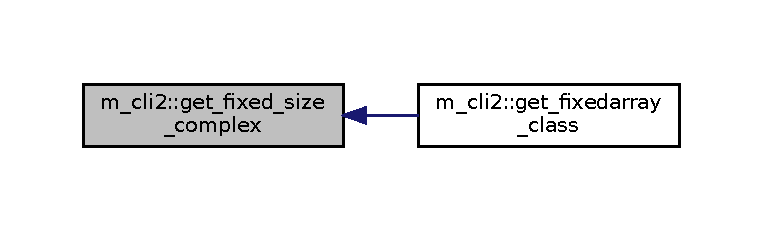
\includegraphics[width=350pt]{namespacem__cli2_a32b78784e20e29bf40f17e16d08336fa_icgraph}
\end{center}
\end{figure}
\mbox{\Hypertarget{namespacem__cli2_a6d8c1c441ac15f9a2882e50459d39565}\label{namespacem__cli2_a6d8c1c441ac15f9a2882e50459d39565}} 
\index{m\_cli2@{m\_cli2}!get\_fixedarray\_class@{get\_fixedarray\_class}}
\index{get\_fixedarray\_class@{get\_fixedarray\_class}!m\_cli2@{m\_cli2}}
\doxysubsubsection{\texorpdfstring{get\_fixedarray\_class()}{get\_fixedarray\_class()}}
{\footnotesize\ttfamily subroutine m\+\_\+cli2\+::get\+\_\+fixedarray\+\_\+class (\begin{DoxyParamCaption}\item[{character(len=$\ast$), intent(in)}]{keyword,  }\item[{class($\ast$), dimension(\+:)}]{generic,  }\item[{character(len=$\ast$), intent(in), optional}]{delimiters }\end{DoxyParamCaption})\hspace{0.3cm}{\ttfamily [private]}}

\hypertarget{namespacem__cli2_autotoc_md86}{}\doxysubsubsection{N\+A\+ME}\label{namespacem__cli2_autotoc_md86}
get\+\_\+args(3f) -\/ \mbox{[}A\+R\+G\+U\+M\+E\+N\+TS\+:M\+\_\+\+C\+L\+I2\mbox{]} return keyword values when parsing command line arguments (L\+I\+C\+E\+N\+SE\+:PD)\hypertarget{namespacem__cli2_autotoc_md87}{}\doxysubsubsection{S\+Y\+N\+O\+P\+S\+IS}\label{namespacem__cli2_autotoc_md87}
\begin{DoxyVerb} use M_CLI2, only : get_args
 ! convenience functions
 use M_CLI2, only : dget, iget, lget, rget, sget, cget
 use M_CLI2, only : dgets, igets, lgets, rgets, sgets, cgets

 subroutine get_args(name,value,delimiters)

  character(len=*),intent(in) :: name

  character(len=:),allocatable :: value
  ! or
  character(len=:),allocatable :: value(:)
  ! or
  [real|doubleprecision|integer|logical|complex] :: value
  ! or
  [real|doubleprecision|integer|logical|complex],allocatable :: value(:)

  character(len=*),intent(in),optional :: delimiters
\end{DoxyVerb}
\hypertarget{namespacem__cli2_autotoc_md88}{}\doxysubsubsection{D\+E\+S\+C\+R\+I\+P\+T\+I\+ON}\label{namespacem__cli2_autotoc_md88}
\begin{DoxyVerb}GET_ARGS(3f) returns the value of keywords after SET_ARGS(3f)
has been called. For fixed-length CHARACTER variables
see GET_ARGS_FIXED_LENGTH(3f). For fixed-size arrays see
GET_ARGS_FIXED_SIZE(3f).

As a convenience multiple pairs of keywords and variables may be
specified if and only if all the values are scalars and the CHARACTER
variables are fixed-length or pre-allocated.
\end{DoxyVerb}
\hypertarget{namespacem__cli2_autotoc_md89}{}\doxysubsubsection{O\+P\+T\+I\+O\+NS}\label{namespacem__cli2_autotoc_md89}
\begin{DoxyVerb} NAME        name of commandline argument to obtain the value of
 VALUE       variable to hold returned value. The kind of the value
             is used to determine the type of returned value. May
             be a scalar or allocatable array. If type is CHARACTER
             the scalar must have an allocatable length.
 DELIMITERS  By default the delimiter for array values are comma,
             colon, and whitespace. A string containing an alternate
             list of delimiter characters may be supplied.
\end{DoxyVerb}
\hypertarget{namespacem__cli2_autotoc_md90}{}\doxysubsubsection{C\+O\+N\+V\+E\+N\+I\+E\+N\+C\+E F\+U\+N\+C\+T\+I\+O\+NS}\label{namespacem__cli2_autotoc_md90}
\begin{DoxyVerb}There are convenience functions that are replacements for calls to
get_args(3f) for each supported default intrinsic type

  o scalars -- dget(3f), iget(3f), lget(3f), rget(3f), sget(3f),
               cget(3f)
  o vectors -- dgets(3f), igets(3f), lgets(3f), rgets(3f),
               sgets(3f), cgets(3f)

D is for DOUBLEPRECISION, I for INTEGER, L for LOGICAL, R for REAL,
S for string (CHARACTER), and C for COMPLEX.

If the functions are called with no argument they will return the
UNNAMED array converted to the specified type.
\end{DoxyVerb}
\hypertarget{namespacem__cli2_autotoc_md91}{}\doxysubsubsection{E\+X\+A\+M\+P\+LE}\label{namespacem__cli2_autotoc_md91}
Sample program\+: \begin{DoxyVerb}program demo_get_args
use M_CLI2,  only : filenames=>unnamed, set_args, get_args
implicit none
integer                      :: i
! DEFINE ARGS
real                         :: x, y, z
real,allocatable             :: p(:)
character(len=:),allocatable :: title
logical                      :: l, lbig
! DEFINE AND PARSE (TO SET INITIAL VALUES) COMMAND LINE
!   o only quote strings and use double-quotes
!   o set all logical values to F or T.
call set_args(' &
   &-x 1 -y 2 -z 3 &
   &-p -1,-2,-3 &
   &--title "my title" &
   & -l F -L F  &
   & --label " " &
   & ')
! ASSIGN VALUES TO ELEMENTS
! SCALARS
call get_args('x',x,'y',y,'z',z)
call get_args('l',l)
call get_args('L',lbig)
! ALLOCATABLE STRING
call get_args('title',title)
! NON-ALLOCATABLE ARRAYS
call get_args('p',p)
! USE VALUES
write(*,'(1x,g0,"=",g0)')'x',x, 'y',y, 'z',z
write(*,*)'p=',p
write(*,*)'title=',title
write(*,*)'l=',l
write(*,*)'L=',lbig
if(size(filenames).gt.0)then
   write(*,'(i6.6,3a)')(i,'[',filenames(i),']',i=1,size(filenames))
endif
end program demo_get_args
\end{DoxyVerb}
 \hypertarget{namespacem__cli2_autotoc_md92}{}\doxysubsubsection{A\+U\+T\+H\+OR}\label{namespacem__cli2_autotoc_md92}
John S. Urban, 2019 \hypertarget{namespacem__cli2_autotoc_md93}{}\doxysubsubsection{L\+I\+C\+E\+N\+SE}\label{namespacem__cli2_autotoc_md93}
Public Domain\hypertarget{namespacem__cli2_autotoc_md94}{}\doxysubsubsection{N\+A\+ME}\label{namespacem__cli2_autotoc_md94}
get\+\_\+args\+\_\+fixed\+\_\+length(3f) -\/ \mbox{[}A\+R\+G\+U\+M\+E\+N\+TS\+:M\+\_\+\+C\+L\+I2\mbox{]} return keyword values for fixed-\/length string when parsing command line (L\+I\+C\+E\+N\+SE\+:PD)\hypertarget{namespacem__cli2_autotoc_md95}{}\doxysubsubsection{S\+Y\+N\+O\+P\+S\+IS}\label{namespacem__cli2_autotoc_md95}
\begin{DoxyVerb}subroutine get_args_fixed_length(name,value)

 character(len=:),allocatable :: value
 character(len=*),intent(in),optional :: delimiters
\end{DoxyVerb}
\hypertarget{namespacem__cli2_autotoc_md96}{}\doxysubsubsection{D\+E\+S\+C\+R\+I\+P\+T\+I\+ON}\label{namespacem__cli2_autotoc_md96}
\begin{DoxyVerb}GET_ARGS_fixed_length(3f) returns the value of a string
keyword when the string value is a fixed-length CHARACTER
variable.
\end{DoxyVerb}
\hypertarget{namespacem__cli2_autotoc_md97}{}\doxysubsubsection{O\+P\+T\+I\+O\+NS}\label{namespacem__cli2_autotoc_md97}
\begin{DoxyVerb}NAME   name of commandline argument to obtain the value of

VALUE  variable to hold returned value.
       Must be a fixed-length CHARACTER variable.

DELIMITERS  By default the delimiter for array values are comma,
            colon, and whitespace. A string containing an alternate
            list of delimiter characters may be supplied.
\end{DoxyVerb}
\hypertarget{namespacem__cli2_autotoc_md98}{}\doxysubsubsection{E\+X\+A\+M\+P\+LE}\label{namespacem__cli2_autotoc_md98}
Sample program\+: \begin{DoxyVerb}program demo_get_args_fixed_length
use M_CLI2,  only : set_args, get_args_fixed_length
implicit none
! DEFINE ARGS
character(len=80)   :: title
call set_args(' &
   & -title "my title" &
   & ')
! ASSIGN VALUES TO ELEMENTS
   call get_args_fixed_length('title',title)
! USE VALUES
   write(*,*)'title=',title
end program demo_get_args_fixed_length
\end{DoxyVerb}
\hypertarget{namespacem__cli2_autotoc_md99}{}\doxysubsubsection{A\+U\+T\+H\+OR}\label{namespacem__cli2_autotoc_md99}
John S. Urban, 2019 \hypertarget{namespacem__cli2_autotoc_md100}{}\doxysubsubsection{L\+I\+C\+E\+N\+SE}\label{namespacem__cli2_autotoc_md100}
Public Domain\hypertarget{namespacem__cli2_autotoc_md101}{}\doxysubsubsection{N\+A\+ME}\label{namespacem__cli2_autotoc_md101}
get\+\_\+args\+\_\+fixed\+\_\+size(3f) -\/ \mbox{[}A\+R\+G\+U\+M\+E\+N\+TS\+:M\+\_\+\+C\+L\+I2\mbox{]} return keyword values for fixed-\/size array when parsing command line arguments (L\+I\+C\+E\+N\+SE\+:PD)\hypertarget{namespacem__cli2_autotoc_md102}{}\doxysubsubsection{S\+Y\+N\+O\+P\+S\+IS}\label{namespacem__cli2_autotoc_md102}
\begin{DoxyVerb}subroutine get_args_fixed_size(name,value)

 [real|doubleprecision|integer|logical|complex] :: value(NNN)
    or
 character(len=MMM) :: value(NNN)

 character(len=*),intent(in),optional :: delimiters
\end{DoxyVerb}
\hypertarget{namespacem__cli2_autotoc_md103}{}\doxysubsubsection{D\+E\+S\+C\+R\+I\+P\+T\+I\+ON}\label{namespacem__cli2_autotoc_md103}
\begin{DoxyVerb}GET_ARGS_FIXED_SIZE(3f) returns the value of keywords for
fixed-size arrays after SET_ARGS(3f) has been called.
On input on the command line all values of the array must
be specified.
\end{DoxyVerb}
\hypertarget{namespacem__cli2_autotoc_md104}{}\doxysubsubsection{O\+P\+T\+I\+O\+NS}\label{namespacem__cli2_autotoc_md104}
N\+A\+ME name of commandline argument to obtain the value of

V\+A\+L\+UE variable to hold returned values. The kind of the value is used to determine the type of returned value. Must be a fixed-\/size array. If type is C\+H\+A\+R\+A\+C\+T\+ER the length must also be fixed.

D\+E\+L\+I\+M\+I\+T\+E\+RS By default the delimiter for array values are comma, colon, and whitespace. A string containing an alternate list of delimiter characters may be supplied.\hypertarget{namespacem__cli2_autotoc_md105}{}\doxysubsubsection{E\+X\+A\+M\+P\+LE}\label{namespacem__cli2_autotoc_md105}
Sample program\+: \begin{DoxyVerb}program demo_get_args_fixed_size
use M_CLI2,  only : set_args, get_args_fixed_size
implicit none
integer,parameter   :: dp=kind(0.0d0)
! DEFINE ARGS
real                :: x(2)
real(kind=dp)       :: y(2)
integer             :: p(3)
character(len=80)   :: title(1)
logical             :: l(4), lbig(4)
complex             :: cmp(2)
! DEFINE AND PARSE (TO SET INITIAL VALUES) COMMAND LINE
!   o only quote strings
!   o set all logical values to F or T.
call set_args(' &
   & -x 10.0,20.0 &
   & -y 11.0,22.0 &
   & -p -1,-2,-3 &
   & -title "my title" &
   & -l F,T,F,T -L T,F,T,F  &
   & --cmp 111,222.0,333.0e0,4444 &
   & ')
! ASSIGN VALUES TO ELEMENTS
   call get_args_fixed_size('x',x)
   call get_args_fixed_size('y',y)
   call get_args_fixed_size('p',p)
   call get_args_fixed_size('title',title)
   call get_args_fixed_size('l',l)
   call get_args_fixed_size('L',lbig)
   call get_args_fixed_size('cmp',cmp)
! USE VALUES
   write(*,*)'x=',x
   write(*,*)'p=',p
   write(*,*)'title=',title
   write(*,*)'l=',l
   write(*,*)'L=',lbig
   write(*,*)'cmp=',cmp
end program demo_get_args_fixed_size
\end{DoxyVerb}
 Results\+:\hypertarget{namespacem__cli2_autotoc_md106}{}\doxysubsubsection{A\+U\+T\+H\+OR}\label{namespacem__cli2_autotoc_md106}
John S. Urban, 2019 \hypertarget{namespacem__cli2_autotoc_md107}{}\doxysubsubsection{L\+I\+C\+E\+N\+SE}\label{namespacem__cli2_autotoc_md107}
Public Domain 

References dp, get\+\_\+fixed\+\_\+size\+\_\+complex(), get\+\_\+fixedarray\+\_\+d(), get\+\_\+fixedarray\+\_\+fixed\+\_\+length\+\_\+c(), get\+\_\+fixedarray\+\_\+i(), get\+\_\+fixedarray\+\_\+l(), get\+\_\+fixedarray\+\_\+r(), and mystop().

Here is the call graph for this function\+:\nopagebreak
\begin{figure}[H]
\begin{center}
\leavevmode
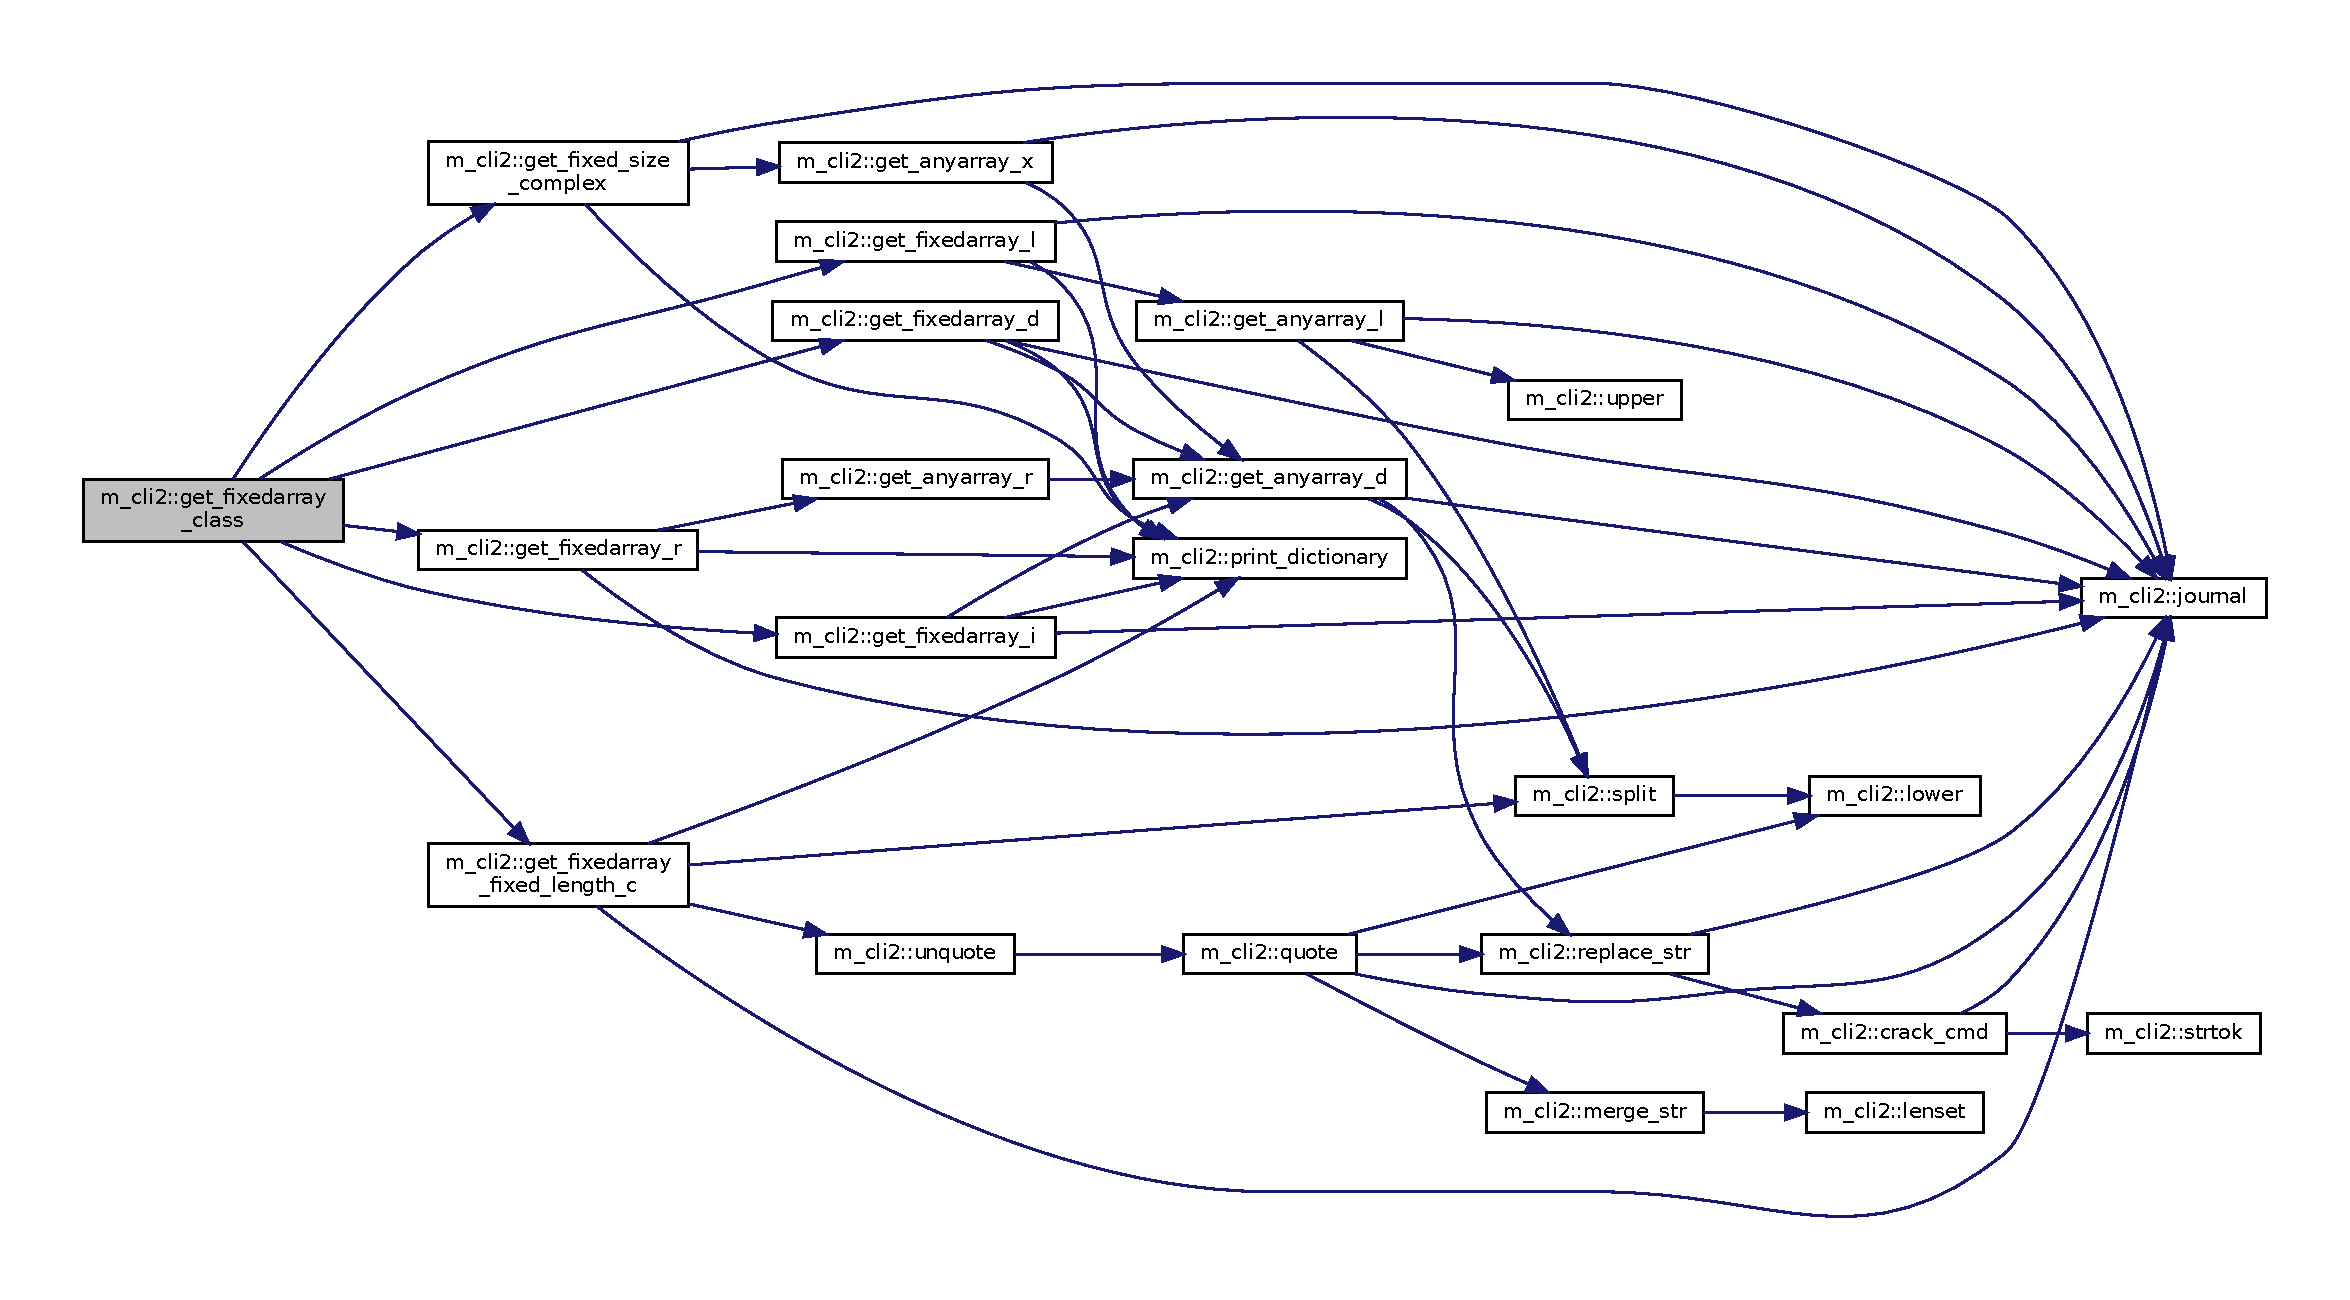
\includegraphics[width=350pt]{namespacem__cli2_a6d8c1c441ac15f9a2882e50459d39565_cgraph}
\end{center}
\end{figure}
\mbox{\Hypertarget{namespacem__cli2_a2c8db0f383888cb2b3ce8643de3fae93}\label{namespacem__cli2_a2c8db0f383888cb2b3ce8643de3fae93}} 
\index{m\_cli2@{m\_cli2}!get\_fixedarray\_d@{get\_fixedarray\_d}}
\index{get\_fixedarray\_d@{get\_fixedarray\_d}!m\_cli2@{m\_cli2}}
\doxysubsubsection{\texorpdfstring{get\_fixedarray\_d()}{get\_fixedarray\_d()}}
{\footnotesize\ttfamily subroutine m\+\_\+cli2\+::get\+\_\+fixedarray\+\_\+d (\begin{DoxyParamCaption}\item[{character(len=$\ast$), intent(in)}]{keyword,  }\item[{real(kind=\mbox{\hyperlink{namespacem__cli2_acf83f1963cf6a56ad0221cfcf5402440}{dp}}), dimension(\+:)}]{darr,  }\item[{character(len=$\ast$), intent(in), optional}]{delimiters }\end{DoxyParamCaption})\hspace{0.3cm}{\ttfamily [private]}}



References get\+\_\+anyarray\+\_\+d(), journal(), mystop(), and print\+\_\+dictionary().

Here is the call graph for this function\+:\nopagebreak
\begin{figure}[H]
\begin{center}
\leavevmode
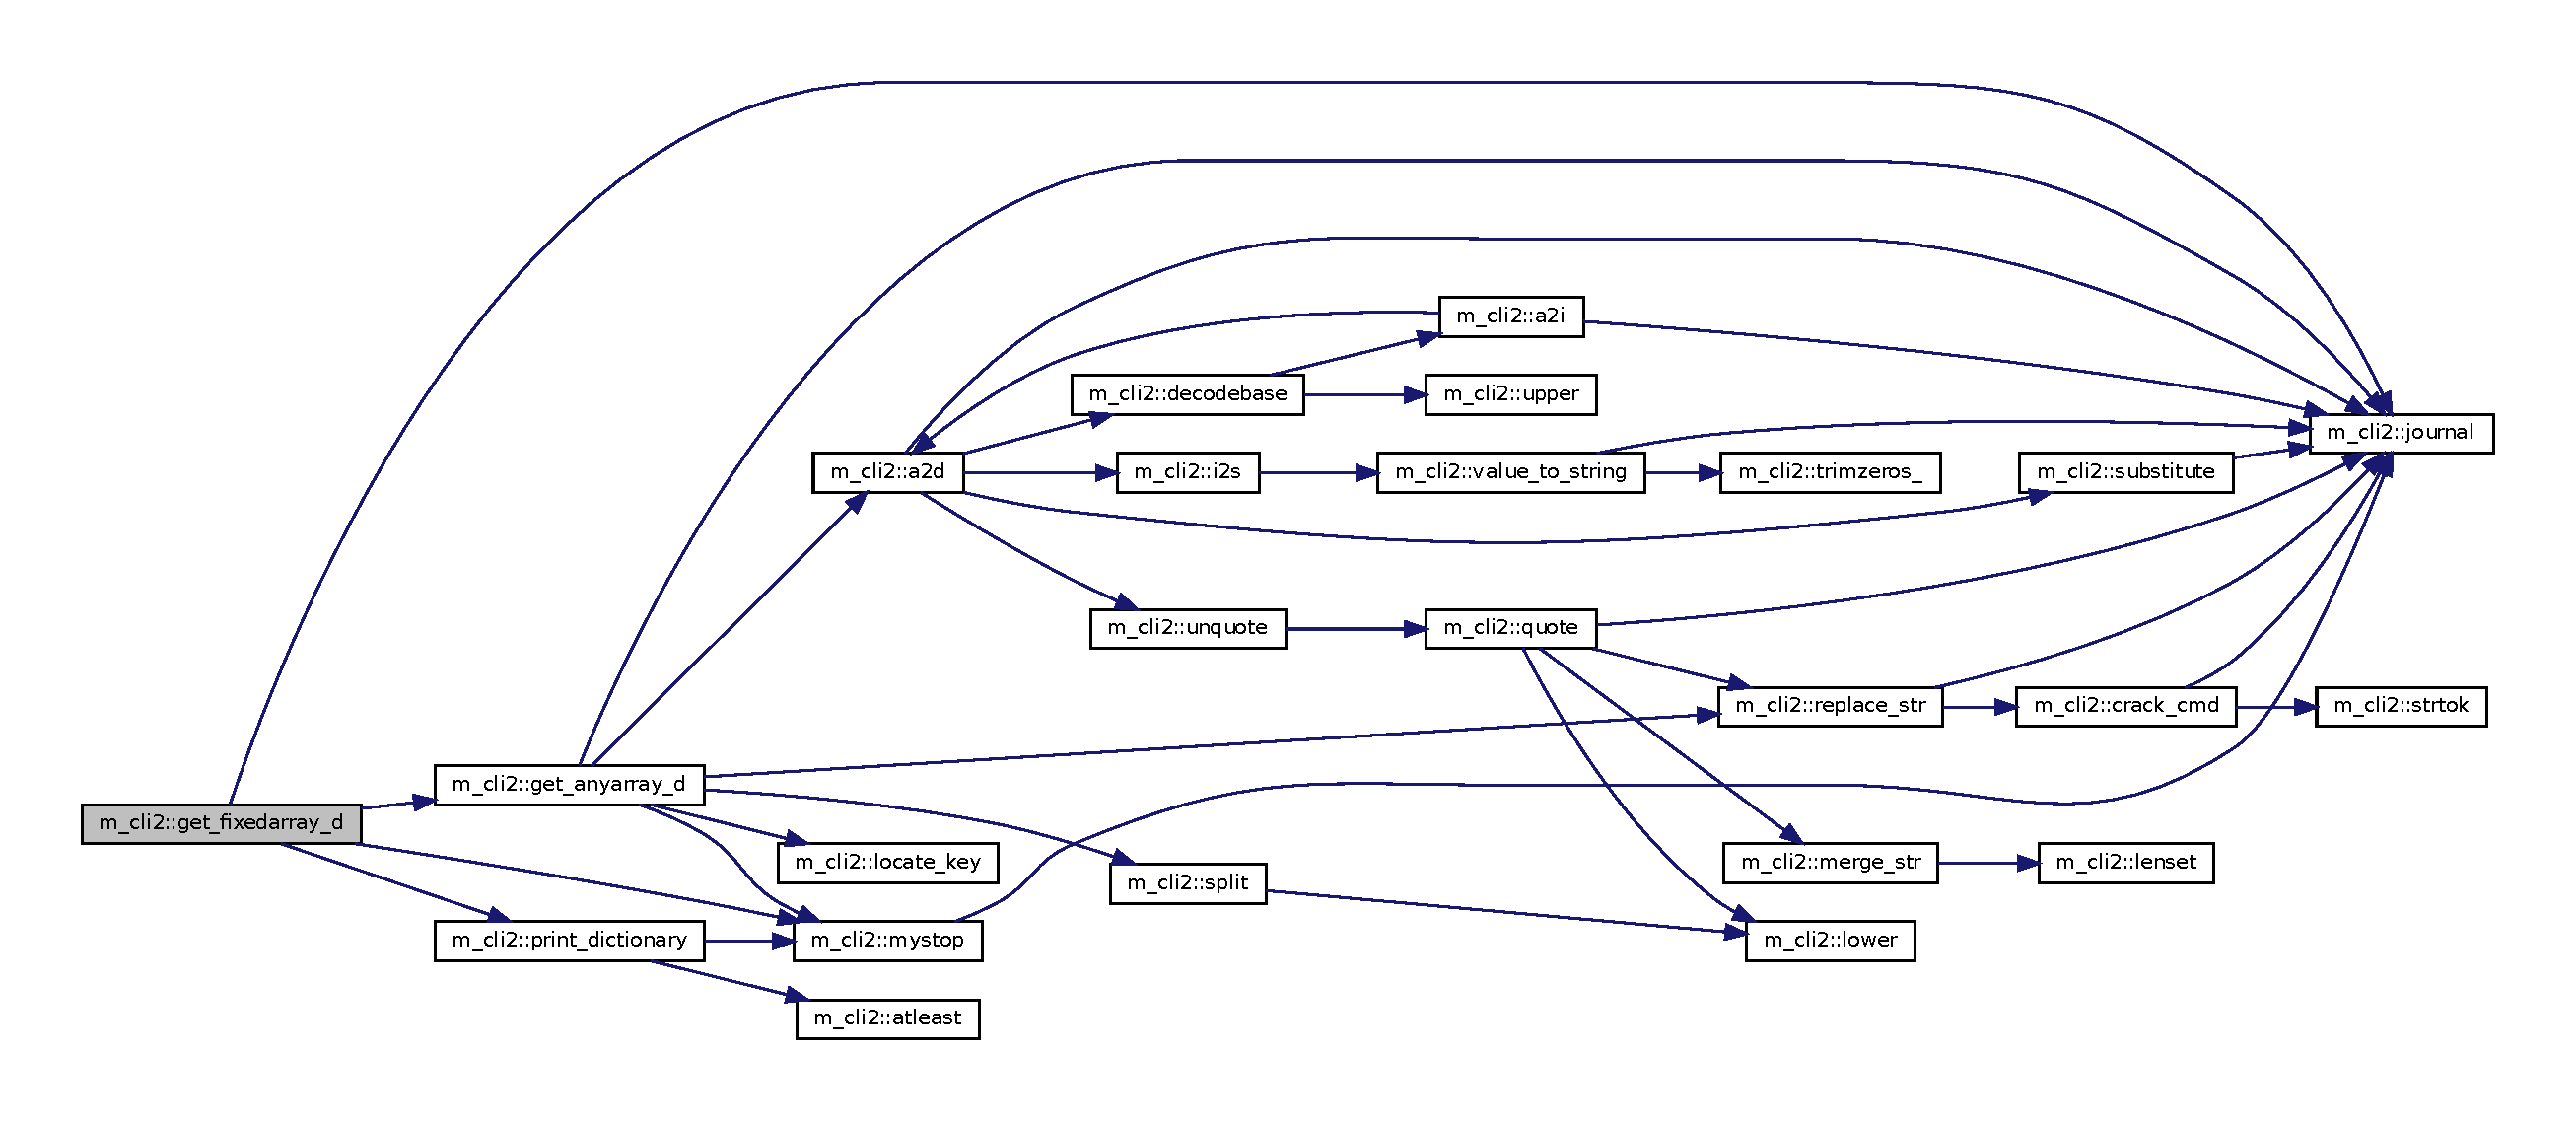
\includegraphics[width=350pt]{namespacem__cli2_a2c8db0f383888cb2b3ce8643de3fae93_cgraph}
\end{center}
\end{figure}
Here is the caller graph for this function\+:\nopagebreak
\begin{figure}[H]
\begin{center}
\leavevmode
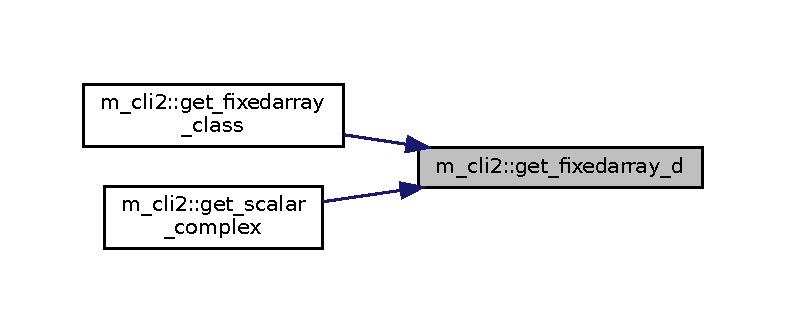
\includegraphics[width=350pt]{namespacem__cli2_a2c8db0f383888cb2b3ce8643de3fae93_icgraph}
\end{center}
\end{figure}
\mbox{\Hypertarget{namespacem__cli2_a8000c5e05f6c84ba17350d4a00850a6a}\label{namespacem__cli2_a8000c5e05f6c84ba17350d4a00850a6a}} 
\index{m\_cli2@{m\_cli2}!get\_fixedarray\_fixed\_length\_c@{get\_fixedarray\_fixed\_length\_c}}
\index{get\_fixedarray\_fixed\_length\_c@{get\_fixedarray\_fixed\_length\_c}!m\_cli2@{m\_cli2}}
\doxysubsubsection{\texorpdfstring{get\_fixedarray\_fixed\_length\_c()}{get\_fixedarray\_fixed\_length\_c()}}
{\footnotesize\ttfamily subroutine m\+\_\+cli2\+::get\+\_\+fixedarray\+\_\+fixed\+\_\+length\+\_\+c (\begin{DoxyParamCaption}\item[{character(len=$\ast$), intent(in)}]{keyword,  }\item[{character(len=$\ast$), dimension(\+:)}]{strings,  }\item[{character(len=$\ast$), intent(in), optional}]{delimiters }\end{DoxyParamCaption})\hspace{0.3cm}{\ttfamily [private]}}



References counts, journal(), locate\+\_\+key(), mystop(), print\+\_\+dictionary(), split(), unquote(), and values.

Here is the call graph for this function\+:\nopagebreak
\begin{figure}[H]
\begin{center}
\leavevmode
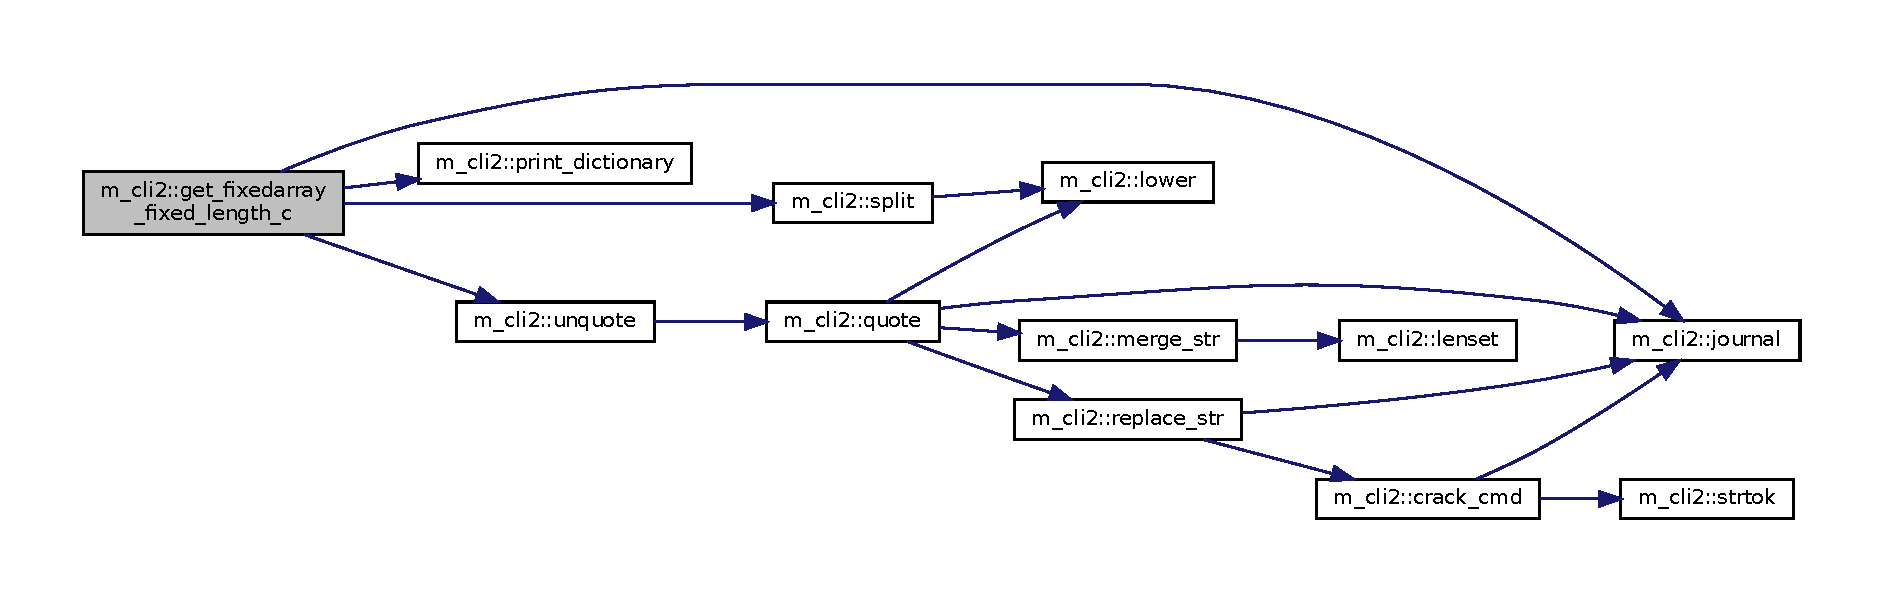
\includegraphics[width=350pt]{namespacem__cli2_a8000c5e05f6c84ba17350d4a00850a6a_cgraph}
\end{center}
\end{figure}
Here is the caller graph for this function\+:\nopagebreak
\begin{figure}[H]
\begin{center}
\leavevmode
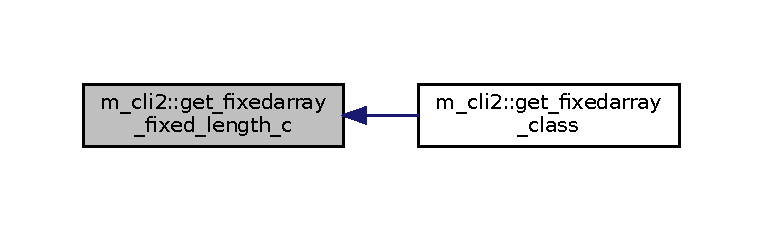
\includegraphics[width=350pt]{namespacem__cli2_a8000c5e05f6c84ba17350d4a00850a6a_icgraph}
\end{center}
\end{figure}
\mbox{\Hypertarget{namespacem__cli2_aa469ba94e6bb122c9bf30dd8642b693b}\label{namespacem__cli2_aa469ba94e6bb122c9bf30dd8642b693b}} 
\index{m\_cli2@{m\_cli2}!get\_fixedarray\_i@{get\_fixedarray\_i}}
\index{get\_fixedarray\_i@{get\_fixedarray\_i}!m\_cli2@{m\_cli2}}
\doxysubsubsection{\texorpdfstring{get\_fixedarray\_i()}{get\_fixedarray\_i()}}
{\footnotesize\ttfamily subroutine m\+\_\+cli2\+::get\+\_\+fixedarray\+\_\+i (\begin{DoxyParamCaption}\item[{character(len=$\ast$), intent(in)}]{keyword,  }\item[{integer, dimension(\+:)}]{iarray,  }\item[{character(len=$\ast$), intent(in), optional}]{delimiters }\end{DoxyParamCaption})\hspace{0.3cm}{\ttfamily [private]}}



References get\+\_\+anyarray\+\_\+d(), journal(), mystop(), and print\+\_\+dictionary().

Here is the call graph for this function\+:\nopagebreak
\begin{figure}[H]
\begin{center}
\leavevmode
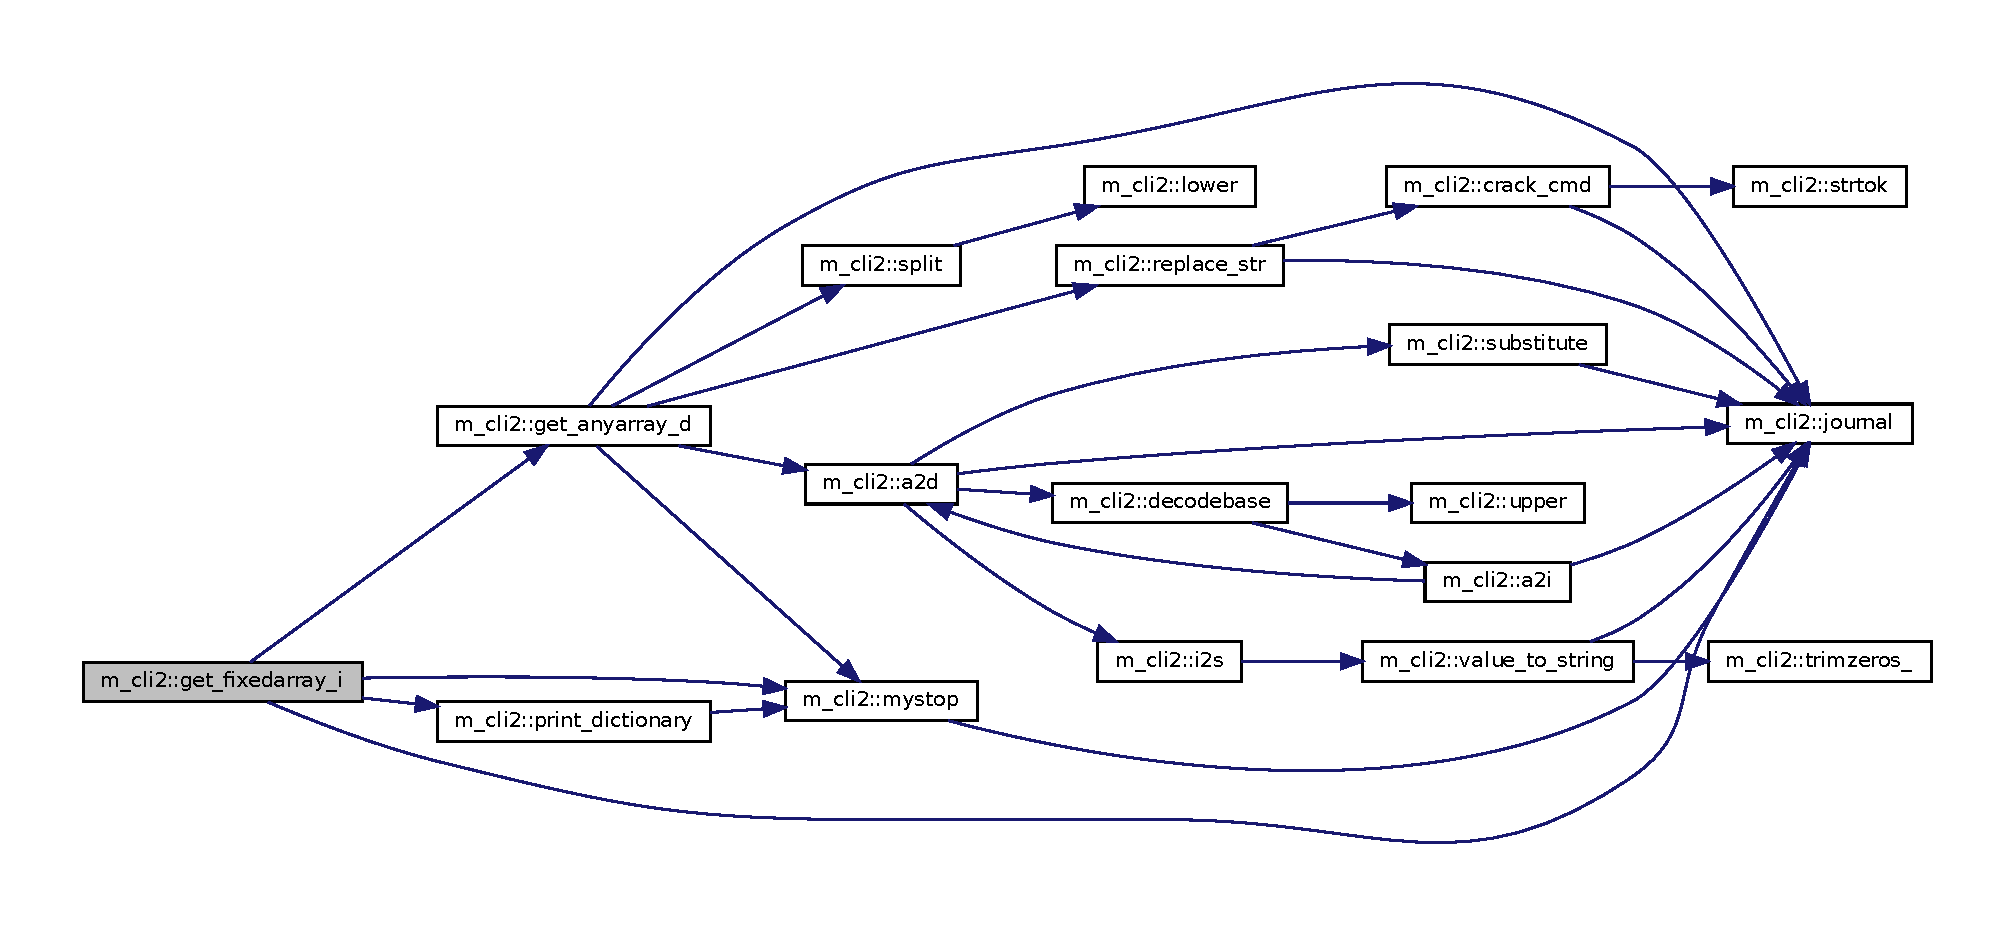
\includegraphics[width=350pt]{namespacem__cli2_aa469ba94e6bb122c9bf30dd8642b693b_cgraph}
\end{center}
\end{figure}
Here is the caller graph for this function\+:\nopagebreak
\begin{figure}[H]
\begin{center}
\leavevmode
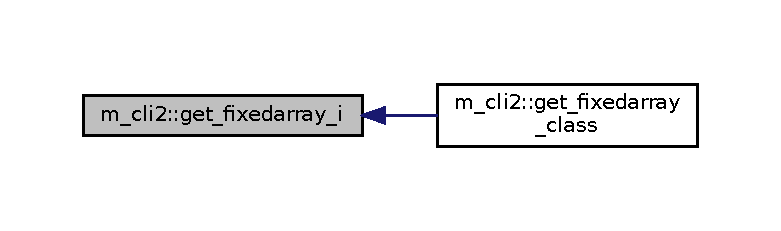
\includegraphics[width=350pt]{namespacem__cli2_aa469ba94e6bb122c9bf30dd8642b693b_icgraph}
\end{center}
\end{figure}
\mbox{\Hypertarget{namespacem__cli2_a65ffe8c7a444db5db3be3f6edecef008}\label{namespacem__cli2_a65ffe8c7a444db5db3be3f6edecef008}} 
\index{m\_cli2@{m\_cli2}!get\_fixedarray\_l@{get\_fixedarray\_l}}
\index{get\_fixedarray\_l@{get\_fixedarray\_l}!m\_cli2@{m\_cli2}}
\doxysubsubsection{\texorpdfstring{get\_fixedarray\_l()}{get\_fixedarray\_l()}}
{\footnotesize\ttfamily subroutine m\+\_\+cli2\+::get\+\_\+fixedarray\+\_\+l (\begin{DoxyParamCaption}\item[{character(len=$\ast$), intent(in)}]{keyword,  }\item[{logical, dimension(\+:)}]{larray,  }\item[{character(len=$\ast$), intent(in), optional}]{delimiters }\end{DoxyParamCaption})\hspace{0.3cm}{\ttfamily [private]}}



References get\+\_\+anyarray\+\_\+l(), journal(), mystop(), and print\+\_\+dictionary().

Here is the call graph for this function\+:\nopagebreak
\begin{figure}[H]
\begin{center}
\leavevmode
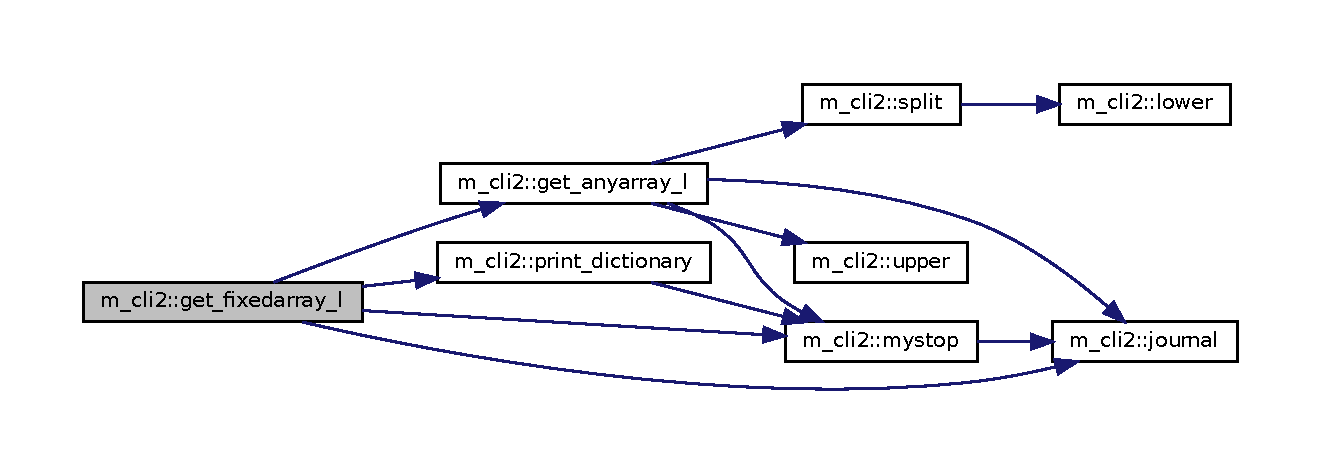
\includegraphics[width=350pt]{namespacem__cli2_a65ffe8c7a444db5db3be3f6edecef008_cgraph}
\end{center}
\end{figure}
Here is the caller graph for this function\+:\nopagebreak
\begin{figure}[H]
\begin{center}
\leavevmode
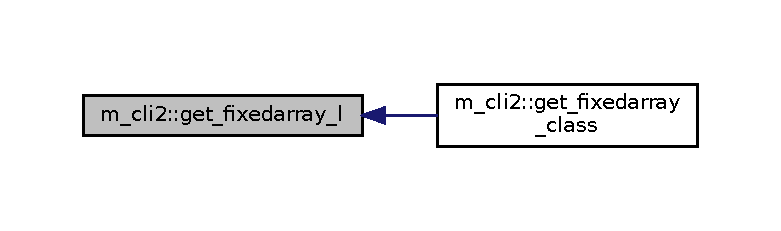
\includegraphics[width=350pt]{namespacem__cli2_a65ffe8c7a444db5db3be3f6edecef008_icgraph}
\end{center}
\end{figure}
\mbox{\Hypertarget{namespacem__cli2_afbec790abad0dca990c0a61cd2d9e9ae}\label{namespacem__cli2_afbec790abad0dca990c0a61cd2d9e9ae}} 
\index{m\_cli2@{m\_cli2}!get\_fixedarray\_r@{get\_fixedarray\_r}}
\index{get\_fixedarray\_r@{get\_fixedarray\_r}!m\_cli2@{m\_cli2}}
\doxysubsubsection{\texorpdfstring{get\_fixedarray\_r()}{get\_fixedarray\_r()}}
{\footnotesize\ttfamily subroutine m\+\_\+cli2\+::get\+\_\+fixedarray\+\_\+r (\begin{DoxyParamCaption}\item[{character(len=$\ast$), intent(in)}]{keyword,  }\item[{real, dimension(\+:)}]{rarray,  }\item[{character(len=$\ast$), intent(in), optional}]{delimiters }\end{DoxyParamCaption})\hspace{0.3cm}{\ttfamily [private]}}



References get\+\_\+anyarray\+\_\+r(), journal(), mystop(), and print\+\_\+dictionary().

Here is the call graph for this function\+:\nopagebreak
\begin{figure}[H]
\begin{center}
\leavevmode
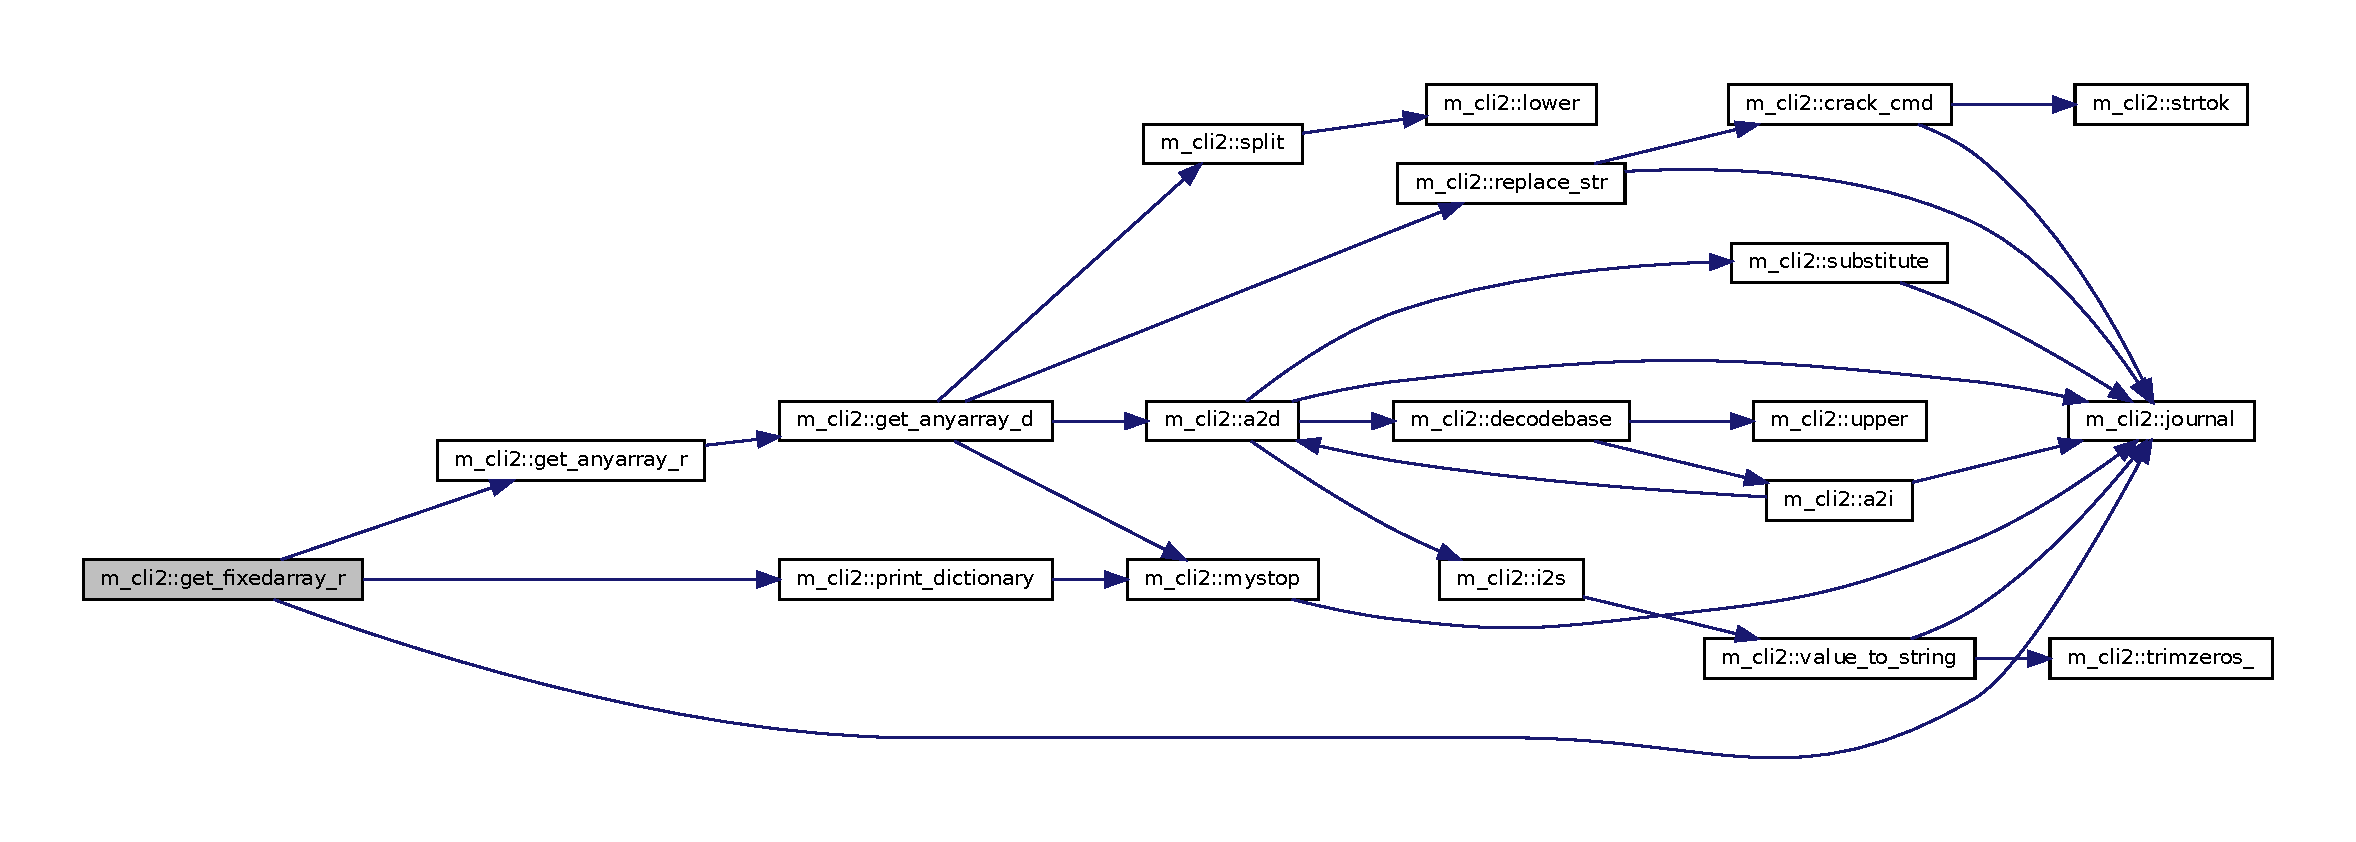
\includegraphics[width=350pt]{namespacem__cli2_afbec790abad0dca990c0a61cd2d9e9ae_cgraph}
\end{center}
\end{figure}
Here is the caller graph for this function\+:\nopagebreak
\begin{figure}[H]
\begin{center}
\leavevmode
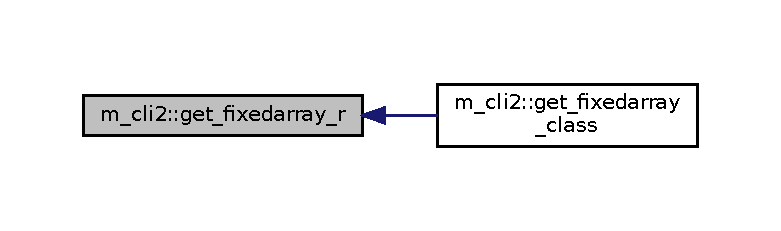
\includegraphics[width=350pt]{namespacem__cli2_afbec790abad0dca990c0a61cd2d9e9ae_icgraph}
\end{center}
\end{figure}
\mbox{\Hypertarget{namespacem__cli2_aa9186cd1cdabb275385314ff152e395e}\label{namespacem__cli2_aa9186cd1cdabb275385314ff152e395e}} 
\index{m\_cli2@{m\_cli2}!get\_name@{get\_name}}
\index{get\_name@{get\_name}!m\_cli2@{m\_cli2}}
\doxysubsubsection{\texorpdfstring{get\_name()}{get\_name()}}
{\footnotesize\ttfamily character(len=\+:) function, allocatable m\+\_\+cli2\+::get\+\_\+name\hspace{0.3cm}{\ttfamily [private]}}

Here is the caller graph for this function\+:\nopagebreak
\begin{figure}[H]
\begin{center}
\leavevmode
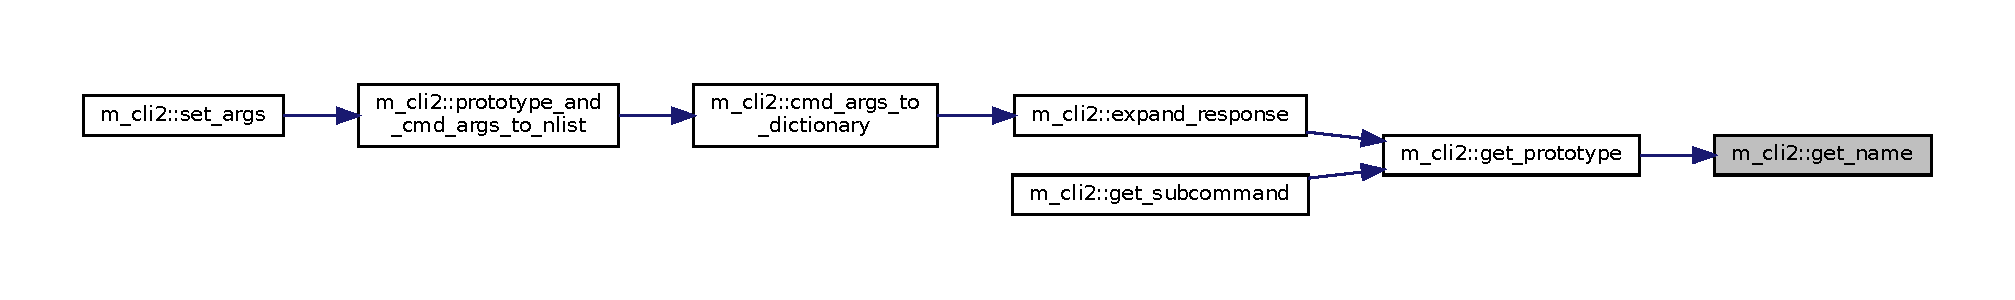
\includegraphics[width=350pt]{namespacem__cli2_aa9186cd1cdabb275385314ff152e395e_icgraph}
\end{center}
\end{figure}
\mbox{\Hypertarget{namespacem__cli2_a6451ae626dec12d6e47dc23c802366a5}\label{namespacem__cli2_a6451ae626dec12d6e47dc23c802366a5}} 
\index{m\_cli2@{m\_cli2}!get\_prototype@{get\_prototype}}
\index{get\_prototype@{get\_prototype}!m\_cli2@{m\_cli2}}
\doxysubsubsection{\texorpdfstring{get\_prototype()}{get\_prototype()}}
{\footnotesize\ttfamily subroutine m\+\_\+cli2\+::get\+\_\+prototype (\begin{DoxyParamCaption}\item[{character(len=$\ast$), intent(in)}]{name,  }\item[{character(len=\+:), intent(out), allocatable}]{prototype }\end{DoxyParamCaption})\hspace{0.3cm}{\ttfamily [private]}}



References basename(), debug\+\_\+m\+\_\+cli2, find\+\_\+and\+\_\+read\+\_\+response\+\_\+file(), gen, get\+\_\+env(), and get\+\_\+name().

Here is the call graph for this function\+:\nopagebreak
\begin{figure}[H]
\begin{center}
\leavevmode
\includegraphics[width=350pt]{namespacem__cli2_a6451ae626dec12d6e47dc23c802366a5_cgraph}
\end{center}
\end{figure}
Here is the caller graph for this function\+:\nopagebreak
\begin{figure}[H]
\begin{center}
\leavevmode
\includegraphics[width=350pt]{namespacem__cli2_a6451ae626dec12d6e47dc23c802366a5_icgraph}
\end{center}
\end{figure}
\mbox{\Hypertarget{namespacem__cli2_a7429381c83a021ba3ffb32ed58e17a0e}\label{namespacem__cli2_a7429381c83a021ba3ffb32ed58e17a0e}} 
\index{m\_cli2@{m\_cli2}!get\_scalar\_anylength\_c@{get\_scalar\_anylength\_c}}
\index{get\_scalar\_anylength\_c@{get\_scalar\_anylength\_c}!m\_cli2@{m\_cli2}}
\doxysubsubsection{\texorpdfstring{get\_scalar\_anylength\_c()}{get\_scalar\_anylength\_c()}}
{\footnotesize\ttfamily subroutine m\+\_\+cli2\+::get\+\_\+scalar\+\_\+anylength\+\_\+c (\begin{DoxyParamCaption}\item[{character(len=$\ast$), intent(in)}]{keyword,  }\item[{character(len=\+:), intent(out), allocatable}]{string }\end{DoxyParamCaption})\hspace{0.3cm}{\ttfamily [private]}}



References counts, journal(), locate\+\_\+key(), mystop(), unquote(), and values.

Here is the call graph for this function\+:\nopagebreak
\begin{figure}[H]
\begin{center}
\leavevmode
\includegraphics[width=350pt]{namespacem__cli2_a7429381c83a021ba3ffb32ed58e17a0e_cgraph}
\end{center}
\end{figure}
\mbox{\Hypertarget{namespacem__cli2_a2af4dd786acb5cb2dbd6e43667109490}\label{namespacem__cli2_a2af4dd786acb5cb2dbd6e43667109490}} 
\index{m\_cli2@{m\_cli2}!get\_scalar\_complex@{get\_scalar\_complex}}
\index{get\_scalar\_complex@{get\_scalar\_complex}!m\_cli2@{m\_cli2}}
\doxysubsubsection{\texorpdfstring{get\_scalar\_complex()}{get\_scalar\_complex()}}
{\footnotesize\ttfamily subroutine m\+\_\+cli2\+::get\+\_\+scalar\+\_\+complex (\begin{DoxyParamCaption}\item[{character(len=$\ast$), intent(in)}]{keyword,  }\item[{complex, intent(out)}]{x }\end{DoxyParamCaption})\hspace{0.3cm}{\ttfamily [private]}}



References get\+\_\+fixedarray\+\_\+d(), journal(), mystop(), and sp.

Here is the call graph for this function\+:\nopagebreak
\begin{figure}[H]
\begin{center}
\leavevmode
\includegraphics[width=350pt]{namespacem__cli2_a2af4dd786acb5cb2dbd6e43667109490_cgraph}
\end{center}
\end{figure}
\mbox{\Hypertarget{namespacem__cli2_a338757660adde093db76b7d5559a1906}\label{namespacem__cli2_a338757660adde093db76b7d5559a1906}} 
\index{m\_cli2@{m\_cli2}!get\_scalar\_d@{get\_scalar\_d}}
\index{get\_scalar\_d@{get\_scalar\_d}!m\_cli2@{m\_cli2}}
\doxysubsubsection{\texorpdfstring{get\_scalar\_d()}{get\_scalar\_d()}}
{\footnotesize\ttfamily subroutine m\+\_\+cli2\+::get\+\_\+scalar\+\_\+d (\begin{DoxyParamCaption}\item[{character(len=$\ast$), intent(in)}]{keyword,  }\item[{real(kind=\mbox{\hyperlink{namespacem__cli2_acf83f1963cf6a56ad0221cfcf5402440}{dp}})}]{d }\end{DoxyParamCaption})\hspace{0.3cm}{\ttfamily [private]}}



References get\+\_\+anyarray\+\_\+d(), journal(), mystop(), and print\+\_\+dictionary().

Here is the call graph for this function\+:\nopagebreak
\begin{figure}[H]
\begin{center}
\leavevmode
\includegraphics[width=350pt]{namespacem__cli2_a338757660adde093db76b7d5559a1906_cgraph}
\end{center}
\end{figure}
Here is the caller graph for this function\+:\nopagebreak
\begin{figure}[H]
\begin{center}
\leavevmode
\includegraphics[width=350pt]{namespacem__cli2_a338757660adde093db76b7d5559a1906_icgraph}
\end{center}
\end{figure}
\mbox{\Hypertarget{namespacem__cli2_a9c5208ef6763da7e68dd1e118bea0b7a}\label{namespacem__cli2_a9c5208ef6763da7e68dd1e118bea0b7a}} 
\index{m\_cli2@{m\_cli2}!get\_scalar\_i@{get\_scalar\_i}}
\index{get\_scalar\_i@{get\_scalar\_i}!m\_cli2@{m\_cli2}}
\doxysubsubsection{\texorpdfstring{get\_scalar\_i()}{get\_scalar\_i()}}
{\footnotesize\ttfamily subroutine m\+\_\+cli2\+::get\+\_\+scalar\+\_\+i (\begin{DoxyParamCaption}\item[{character(len=$\ast$), intent(in)}]{keyword,  }\item[{integer, intent(out)}]{i }\end{DoxyParamCaption})\hspace{0.3cm}{\ttfamily [private]}}



References get\+\_\+scalar\+\_\+d().

Here is the call graph for this function\+:\nopagebreak
\begin{figure}[H]
\begin{center}
\leavevmode
\includegraphics[width=350pt]{namespacem__cli2_a9c5208ef6763da7e68dd1e118bea0b7a_cgraph}
\end{center}
\end{figure}
\mbox{\Hypertarget{namespacem__cli2_a138d07d14246ee532ce36e67719e8c7d}\label{namespacem__cli2_a138d07d14246ee532ce36e67719e8c7d}} 
\index{m\_cli2@{m\_cli2}!get\_scalar\_logical@{get\_scalar\_logical}}
\index{get\_scalar\_logical@{get\_scalar\_logical}!m\_cli2@{m\_cli2}}
\doxysubsubsection{\texorpdfstring{get\_scalar\_logical()}{get\_scalar\_logical()}}
{\footnotesize\ttfamily subroutine m\+\_\+cli2\+::get\+\_\+scalar\+\_\+logical (\begin{DoxyParamCaption}\item[{character(len=$\ast$), intent(in)}]{keyword,  }\item[{logical}]{l }\end{DoxyParamCaption})\hspace{0.3cm}{\ttfamily [private]}}



References get\+\_\+anyarray\+\_\+l(), journal(), and mystop().

Here is the call graph for this function\+:\nopagebreak
\begin{figure}[H]
\begin{center}
\leavevmode
\includegraphics[width=350pt]{namespacem__cli2_a138d07d14246ee532ce36e67719e8c7d_cgraph}
\end{center}
\end{figure}
\mbox{\Hypertarget{namespacem__cli2_ad089d91c66626de91bcda84523e80b54}\label{namespacem__cli2_ad089d91c66626de91bcda84523e80b54}} 
\index{m\_cli2@{m\_cli2}!get\_scalar\_real@{get\_scalar\_real}}
\index{get\_scalar\_real@{get\_scalar\_real}!m\_cli2@{m\_cli2}}
\doxysubsubsection{\texorpdfstring{get\_scalar\_real()}{get\_scalar\_real()}}
{\footnotesize\ttfamily subroutine m\+\_\+cli2\+::get\+\_\+scalar\+\_\+real (\begin{DoxyParamCaption}\item[{character(len=$\ast$), intent(in)}]{keyword,  }\item[{real, intent(out)}]{r }\end{DoxyParamCaption})\hspace{0.3cm}{\ttfamily [private]}}



References get\+\_\+scalar\+\_\+d().

Here is the call graph for this function\+:\nopagebreak
\begin{figure}[H]
\begin{center}
\leavevmode
\includegraphics[width=350pt]{namespacem__cli2_ad089d91c66626de91bcda84523e80b54_cgraph}
\end{center}
\end{figure}
\mbox{\Hypertarget{namespacem__cli2_a6ffc050a2aecbb7982180b2752056063}\label{namespacem__cli2_a6ffc050a2aecbb7982180b2752056063}} 
\index{m\_cli2@{m\_cli2}!get\_subcommand@{get\_subcommand}}
\index{get\_subcommand@{get\_subcommand}!m\_cli2@{m\_cli2}}
\doxysubsubsection{\texorpdfstring{get\_subcommand()}{get\_subcommand()}}
{\footnotesize\ttfamily character(len=\+:) function, allocatable, public m\+\_\+cli2\+::get\+\_\+subcommand}

\hypertarget{namespacem__cli2_autotoc_md26}{}\doxysubsubsection{N\+A\+ME}\label{namespacem__cli2_autotoc_md26}
get\+\_\+subcommand(3f) -\/ \mbox{[}A\+R\+G\+U\+M\+E\+N\+TS\+:M\+\_\+\+C\+L\+I2\mbox{]} special-\/case routine for handling subcommands on a command line (L\+I\+C\+E\+N\+SE\+:PD)\hypertarget{namespacem__cli2_autotoc_md27}{}\doxysubsubsection{S\+Y\+N\+O\+P\+S\+IS}\label{namespacem__cli2_autotoc_md27}
\begin{DoxyVerb}function get_subcommand()

 character(len=:),allocatable :: get_subcommand
\end{DoxyVerb}
\hypertarget{namespacem__cli2_autotoc_md28}{}\doxysubsubsection{D\+E\+S\+C\+R\+I\+P\+T\+I\+ON}\label{namespacem__cli2_autotoc_md28}
In the special case when creating a program with subcommands it is assumed the first word on the command line is the subcommand. A routine is required to handle response file processing, therefore this routine (optionally processing response files) returns that first word as the subcommand name.

It should not be used by programs not building a more elaborate command with subcommands.\hypertarget{namespacem__cli2_autotoc_md29}{}\doxysubsubsection{R\+E\+T\+U\+R\+NS}\label{namespacem__cli2_autotoc_md29}
N\+A\+ME name of subcommand\hypertarget{namespacem__cli2_autotoc_md30}{}\doxysubsubsection{E\+X\+A\+M\+P\+LE}\label{namespacem__cli2_autotoc_md30}
Sample program\+:

program demo\+\_\+get\+\_\+subcommand !x! S\+U\+B\+C\+O\+M\+M\+A\+N\+DS !x! For a command with subcommands like git(1) !x! you can make separate namelists for each subcommand. !x! You can call this program which has two subcommands (run, test), !x! like this\+: !x! demo\+\_\+get\+\_\+subcommand --help !x! demo\+\_\+get\+\_\+subcommand run -\/x -\/y -\/z -\/title -\/l -\/L !x! demo\+\_\+get\+\_\+subcommand test -\/title -\/l -\/L -\/testname !x! demo\+\_\+get\+\_\+subcommand run --help implicit none !x! D\+E\+F\+I\+NE V\+A\+L\+U\+ES TO U\+SE AS A\+R\+G\+U\+M\+E\+N\+TS W\+I\+TH I\+N\+I\+T\+I\+AL V\+A\+L\+U\+ES real \+:: x=-\/999.\+0,y=-\/999.\+0,z=-\/999.\+0 character(len=80) \+:: title=\char`\"{}not set\char`\"{} logical \+:: l=.false. logical \+:: l\+\_\+=.false. character(len=80) \+:: testname=\char`\"{}not set\char`\"{} character(len=20) \+:: name call parse(name) !x! D\+E\+F\+I\+NE A\+ND P\+A\+R\+SE C\+O\+M\+M\+A\+ND L\+I\+NE !x! A\+LL D\+O\+NE C\+R\+A\+C\+K\+I\+NG T\+HE C\+O\+M\+M\+A\+ND L\+I\+NE. !x! U\+SE T\+HE V\+A\+L\+U\+ES IN Y\+O\+UR P\+R\+O\+G\+R\+AM. write($\ast$,$\ast$)\textquotesingle{}command was \textquotesingle{},name write($\ast$,$\ast$)\textquotesingle{}x,y,z .... \textquotesingle{},x,y,z write($\ast$,$\ast$)\textquotesingle{}title .... \textquotesingle{},title write($\ast$,$\ast$)\textquotesingle{}l,l\+\_\+ ..... \textquotesingle{},l,l\+\_\+ write($\ast$,$\ast$)\textquotesingle{}testname . \textquotesingle{},testname contains subroutine parse(name) !x! P\+UT E\+V\+E\+R\+Y\+T\+H\+I\+NG TO DO W\+I\+TH C\+O\+M\+M\+A\+ND P\+A\+R\+S\+I\+NG H\+E\+RE F\+OR C\+L\+A\+R\+I\+TY use M\+\_\+\+C\+L\+I2, only \+: set\+\_\+args, \mbox{\hyperlink{interfacem__cli2_1_1get__args}{get\+\_\+args}}, \mbox{\hyperlink{interfacem__cli2_1_1get__args__fixed__length}{get\+\_\+args\+\_\+fixed\+\_\+length}} use M\+\_\+\+C\+L\+I2, only \+: get\+\_\+subcommand use M\+\_\+\+C\+L\+I2, only \+: C\+L\+I\+\_\+\+R\+E\+S\+P\+O\+N\+S\+E\+\_\+\+F\+I\+LE character(len=$\ast$) \+:: name ! the subcommand name character(len=\+:),allocatable \+:: help\+\_\+text(\+:), version\+\_\+text(\+:) C\+L\+I\+\_\+\+R\+E\+S\+P\+O\+N\+S\+E\+\_\+\+F\+I\+LE=.true. ! define version text version\+\_\+text=\mbox{[}character(len=80) \+:: \& \textquotesingle{}@(\#)P\+R\+O\+G\+R\+AM\+: demo\+\_\+get\+\_\+subcommand $>$\textquotesingle{}, \& \textquotesingle{}@(\#)D\+E\+S\+C\+R\+I\+P\+T\+I\+ON\+: My demo program $>$\textquotesingle{}, \& \textquotesingle{}@(\#)V\+E\+R\+S\+I\+ON\+: 1.\+0 20200715 $>$\textquotesingle{}, \& \textquotesingle{}@(\#)A\+U\+T\+H\+OR\+: me, myself, and I$>$\textquotesingle{}, \& \textquotesingle{}@(\#)L\+I\+C\+E\+N\+SE\+: Public Domain $>$\textquotesingle{}, \& \textquotesingle{}\textquotesingle{} \mbox{]} ! general help for \char`\"{}demo\+\_\+get\+\_\+subcommand -\/-\/help\char`\"{} help\+\_\+text=\mbox{[}character(len=80) \+:: \& \textquotesingle{} allowed subcommands are \textquotesingle{}, \& \textquotesingle{} $\ast$ run -\/l -\/L -\/title -\/x -\/y -\/z \textquotesingle{}, \& \textquotesingle{} $\ast$ test -\/l -\/L -\/title \textquotesingle{}, \& \textquotesingle{}\textquotesingle{} \mbox{]} ! find the subcommand name by looking for first word on command ! not starting with dash name = \mbox{\hyperlink{namespacem__cli2_a6ffc050a2aecbb7982180b2752056063}{get\+\_\+subcommand()}} select case(name) case(\textquotesingle{}run\textquotesingle{}) help\+\_\+text=\mbox{[}character(len=80) \+:: \& \textquotesingle{} \textquotesingle{}, \& \textquotesingle{} Help for subcommand \char`\"{}run\char`\"{} \textquotesingle{}, \& \textquotesingle{} \textquotesingle{}, \& \textquotesingle{}\textquotesingle{} \mbox{]} call set\+\_\+args( \& \& \textquotesingle{}-\/x 1 -\/y 2 -\/z 3 --title \char`\"{}my title\char`\"{} -\/l F -\/L F\textquotesingle{},\& \& help\+\_\+text,version\+\_\+text) call \mbox{\hyperlink{interfacem__cli2_1_1get__args}{get\+\_\+args}}(\textquotesingle{}x\textquotesingle{},x) call \mbox{\hyperlink{interfacem__cli2_1_1get__args}{get\+\_\+args}}(\textquotesingle{}y\textquotesingle{},y) call \mbox{\hyperlink{interfacem__cli2_1_1get__args}{get\+\_\+args}}(\textquotesingle{}z\textquotesingle{},z) call \mbox{\hyperlink{interfacem__cli2_1_1get__args__fixed__length}{get\+\_\+args\+\_\+fixed\+\_\+length}}(\textquotesingle{}title\textquotesingle{},title) call \mbox{\hyperlink{interfacem__cli2_1_1get__args}{get\+\_\+args}}(\textquotesingle{}l\textquotesingle{},l) call \mbox{\hyperlink{interfacem__cli2_1_1get__args}{get\+\_\+args}}(\textquotesingle{}L\textquotesingle{},l\+\_\+) case(\textquotesingle{}test\textquotesingle{}) help\+\_\+text=\mbox{[}character(len=80) \+:: \& \textquotesingle{} \textquotesingle{}, \& \textquotesingle{} Help for subcommand \char`\"{}test\char`\"{} \textquotesingle{}, \& \textquotesingle{} \textquotesingle{}, \& \textquotesingle{}\textquotesingle{} \mbox{]} call set\+\_\+args(\& \& \textquotesingle{}--title \char`\"{}my title\char`\"{} -\/l F -\/L F --testname \char`\"{}\+Test\char`\"{}\textquotesingle{},\& \& help\+\_\+text,version\+\_\+text) call \mbox{\hyperlink{interfacem__cli2_1_1get__args__fixed__length}{get\+\_\+args\+\_\+fixed\+\_\+length}}(\textquotesingle{}title\textquotesingle{},title) call \mbox{\hyperlink{interfacem__cli2_1_1get__args}{get\+\_\+args}}(\textquotesingle{}l\textquotesingle{},l) call \mbox{\hyperlink{interfacem__cli2_1_1get__args}{get\+\_\+args}}(\textquotesingle{}L\textquotesingle{},l\+\_\+) call \mbox{\hyperlink{interfacem__cli2_1_1get__args__fixed__length}{get\+\_\+args\+\_\+fixed\+\_\+length}}(\textquotesingle{}testname\textquotesingle{},testname) case default ! process help and version call set\+\_\+args(\textquotesingle{} \textquotesingle{},help\+\_\+text,version\+\_\+text) write($\ast$,\textquotesingle{}($\ast$(a))\textquotesingle{})\textquotesingle{}unknown or missing subcommand \mbox{[}\textquotesingle{},trim(name),\textquotesingle{}\mbox{]}\textquotesingle{} write($\ast$,\textquotesingle{}(a)\textquotesingle{})\mbox{[}character(len=80) \+:: \& \textquotesingle{} allowed subcommands are \textquotesingle{}, \& \textquotesingle{} $\ast$ run -\/l -\/L -\/title -\/x -\/y -\/z \textquotesingle{}, \& \textquotesingle{} $\ast$ test -\/l -\/L -\/title \textquotesingle{}, \& \textquotesingle{}\textquotesingle{} \mbox{]} stop end select end subroutine parse end program demo\+\_\+get\+\_\+subcommand\hypertarget{namespacem__cli2_autotoc_md31}{}\doxysubsubsection{A\+U\+T\+H\+OR}\label{namespacem__cli2_autotoc_md31}
John S. Urban, 2019\hypertarget{namespacem__cli2_autotoc_md32}{}\doxysubsubsection{L\+I\+C\+E\+N\+SE}\label{namespacem__cli2_autotoc_md32}
Public Domain 

References g\+\_\+options\+\_\+only, g\+\_\+subcommand, get\+\_\+prototype(), longest\+\_\+command\+\_\+argument(), split(), and unnamed.

Here is the call graph for this function\+:\nopagebreak
\begin{figure}[H]
\begin{center}
\leavevmode
\includegraphics[width=350pt]{namespacem__cli2_a6ffc050a2aecbb7982180b2752056063_cgraph}
\end{center}
\end{figure}
\mbox{\Hypertarget{namespacem__cli2_aa106d3533fd6d4845f0b3e94b2a79ffb}\label{namespacem__cli2_aa106d3533fd6d4845f0b3e94b2a79ffb}} 
\index{m\_cli2@{m\_cli2}!i2s@{i2s}}
\index{i2s@{i2s}!m\_cli2@{m\_cli2}}
\doxysubsubsection{\texorpdfstring{i2s()}{i2s()}}
{\footnotesize\ttfamily character(len=\+:) function, allocatable m\+\_\+cli2\+::i2s (\begin{DoxyParamCaption}\item[{integer, intent(in)}]{ivalue,  }\item[{character(len=$\ast$), intent(in), optional}]{fmt }\end{DoxyParamCaption})\hspace{0.3cm}{\ttfamily [private]}}



References value\+\_\+to\+\_\+string().

Here is the call graph for this function\+:\nopagebreak
\begin{figure}[H]
\begin{center}
\leavevmode
\includegraphics[width=350pt]{namespacem__cli2_aa106d3533fd6d4845f0b3e94b2a79ffb_cgraph}
\end{center}
\end{figure}
Here is the caller graph for this function\+:\nopagebreak
\begin{figure}[H]
\begin{center}
\leavevmode
\includegraphics[width=350pt]{namespacem__cli2_aa106d3533fd6d4845f0b3e94b2a79ffb_icgraph}
\end{center}
\end{figure}
\mbox{\Hypertarget{namespacem__cli2_a11c3cc864e613c90b2a02c7409c00828}\label{namespacem__cli2_a11c3cc864e613c90b2a02c7409c00828}} 
\index{m\_cli2@{m\_cli2}!ig@{ig}}
\index{ig@{ig}!m\_cli2@{m\_cli2}}
\doxysubsubsection{\texorpdfstring{ig()}{ig()}}
{\footnotesize\ttfamily integer function, dimension(\+:), allocatable m\+\_\+cli2\+::ig\hspace{0.3cm}{\ttfamily [private]}}



References a2i(), and unnamed.

Here is the call graph for this function\+:\nopagebreak
\begin{figure}[H]
\begin{center}
\leavevmode
\includegraphics[width=350pt]{namespacem__cli2_a11c3cc864e613c90b2a02c7409c00828_cgraph}
\end{center}
\end{figure}
\mbox{\Hypertarget{namespacem__cli2_a1b41630a5b78ed0fcb6b6df49ac7738d}\label{namespacem__cli2_a1b41630a5b78ed0fcb6b6df49ac7738d}} 
\index{m\_cli2@{m\_cli2}!iget@{iget}}
\index{iget@{iget}!m\_cli2@{m\_cli2}}
\doxysubsubsection{\texorpdfstring{iget()}{iget()}}
{\footnotesize\ttfamily integer function, public m\+\_\+cli2\+::iget (\begin{DoxyParamCaption}\item[{character(len=$\ast$), intent(in)}]{n }\end{DoxyParamCaption})}

\mbox{\Hypertarget{namespacem__cli2_a39e18c9b881ea554d6d0adee0f5a5313}\label{namespacem__cli2_a39e18c9b881ea554d6d0adee0f5a5313}} 
\index{m\_cli2@{m\_cli2}!igs@{igs}}
\index{igs@{igs}!m\_cli2@{m\_cli2}}
\doxysubsubsection{\texorpdfstring{igs()}{igs()}}
{\footnotesize\ttfamily integer function, dimension(\+:), allocatable m\+\_\+cli2\+::igs (\begin{DoxyParamCaption}\item[{character(len=$\ast$), intent(in)}]{n }\end{DoxyParamCaption})\hspace{0.3cm}{\ttfamily [private]}}

\mbox{\Hypertarget{namespacem__cli2_ab3f2aa827b3b7ff419bcdc3ccb2672b3}\label{namespacem__cli2_ab3f2aa827b3b7ff419bcdc3ccb2672b3}} 
\index{m\_cli2@{m\_cli2}!insert\_c@{insert\_c}}
\index{insert\_c@{insert\_c}!m\_cli2@{m\_cli2}}
\doxysubsubsection{\texorpdfstring{insert\_c()}{insert\_c()}}
{\footnotesize\ttfamily subroutine, private m\+\_\+cli2\+::insert\+\_\+c (\begin{DoxyParamCaption}\item[{character(len=\+:), dimension(\+:), allocatable}]{list,  }\item[{character(len=$\ast$), intent(in)}]{value,  }\item[{integer, intent(in)}]{place }\end{DoxyParamCaption})\hspace{0.3cm}{\ttfamily [private]}}

\hypertarget{namespacem__cli2_autotoc_md224}{}\doxysubsubsection{N\+A\+ME}\label{namespacem__cli2_autotoc_md224}
insert(3f) -\/ \mbox{[}M\+\_\+\+C\+L\+I2\mbox{]} insert entry into a string array at specified position (L\+I\+C\+E\+N\+SE\+:PD)\hypertarget{namespacem__cli2_autotoc_md225}{}\doxysubsubsection{S\+Y\+N\+O\+P\+S\+IS}\label{namespacem__cli2_autotoc_md225}
subroutine insert(list,value,place)

character(len=$\ast$)$\vert$doubleprecision$\vert$real$\vert$integer,intent(in) \+:: value character(len=\+:)$\vert$doubleprecision$\vert$real$\vert$integer,intent(in) \+:: list(\+:) integer,intent(in) \+:: place\hypertarget{namespacem__cli2_autotoc_md226}{}\doxysubsubsection{D\+E\+S\+C\+R\+I\+P\+T\+I\+ON}\label{namespacem__cli2_autotoc_md226}
\begin{DoxyVerb}Insert a value into an allocatable array at the specified index.
The list and value must be of the same type (CHARACTER, DOUBLEPRECISION,
REAL, or INTEGER)
\end{DoxyVerb}
\hypertarget{namespacem__cli2_autotoc_md227}{}\doxysubsubsection{O\+P\+T\+I\+O\+NS}\label{namespacem__cli2_autotoc_md227}
\begin{DoxyVerb}list    is the list array. Must be sorted in descending order.
value   the value to place in the array
PLACE   is the subscript that the entry should be placed at
\end{DoxyVerb}
\hypertarget{namespacem__cli2_autotoc_md228}{}\doxysubsubsection{E\+X\+A\+M\+P\+L\+ES}\label{namespacem__cli2_autotoc_md228}
Find if a string is in a sorted array, and insert the string into the list if it is not present ... \begin{DoxyVerb}program demo_insert
use M_sort, only : sort_shell
use M_CLI2, only : locate, insert
implicit none
character(len=:),allocatable :: arr(:)
integer                       :: i

arr=[character(len=20) :: '', 'ZZZ', 'aaa', 'b', 'xxx' ]
! make sure sorted in descending order
call sort_shell(arr,order='d')
! add or replace values
call update(arr,'b')
call update(arr,'[')
call update(arr,'c')
call update(arr,'ZZ')
call update(arr,'ZZZ')
call update(arr,'ZZZZ')
call update(arr,'')
call update(arr,'z')

contains
subroutine update(arr,string)
character(len=:),allocatable :: arr(:)
character(len=*)             :: string
integer                      :: place, end

end=size(arr)
! find where string is or should be
call locate(arr,string,place)
! if string was not found insert it
if(place.lt.1)then
   call insert(arr,string,abs(place))
endif
! show array
end=size(arr)
write(*,'("array is now SIZE=",i0,1x,*(a,","))')end,(trim(arr(i)),i=1,end)

end subroutine update
end program demo_insert
\end{DoxyVerb}


Results\+:

array is now S\+I\+ZE=5 xxx,b,aaa,Z\+ZZ,, array is now S\+I\+ZE=6 xxx,b,aaa,\mbox{[},Z\+ZZ,, array is now S\+I\+ZE=7 xxx,c,b,aaa,\mbox{[},Z\+ZZ,, array is now S\+I\+ZE=8 xxx,c,b,aaa,\mbox{[},Z\+ZZ,ZZ,, array is now S\+I\+ZE=9 xxx,c,b,aaa,\mbox{[},Z\+Z\+ZZ,Z\+ZZ,ZZ,, array is now S\+I\+ZE=10 z,xxx,c,b,aaa,\mbox{[},Z\+Z\+ZZ,Z\+ZZ,ZZ,,\hypertarget{namespacem__cli2_autotoc_md229}{}\doxysubsubsection{A\+U\+T\+H\+OR}\label{namespacem__cli2_autotoc_md229}
1989,2017 John S. Urban \hypertarget{namespacem__cli2_autotoc_md230}{}\doxysubsubsection{L\+I\+C\+E\+N\+SE}\label{namespacem__cli2_autotoc_md230}
Public Domain \mbox{\Hypertarget{namespacem__cli2_afa6f00a57f1252ba5daa0c440a23ffbb}\label{namespacem__cli2_afa6f00a57f1252ba5daa0c440a23ffbb}} 
\index{m\_cli2@{m\_cli2}!insert\_i@{insert\_i}}
\index{insert\_i@{insert\_i}!m\_cli2@{m\_cli2}}
\doxysubsubsection{\texorpdfstring{insert\_i()}{insert\_i()}}
{\footnotesize\ttfamily subroutine, private m\+\_\+cli2\+::insert\+\_\+i (\begin{DoxyParamCaption}\item[{integer, dimension(\+:), allocatable}]{list,  }\item[{integer, intent(in)}]{value,  }\item[{integer, intent(in)}]{place }\end{DoxyParamCaption})\hspace{0.3cm}{\ttfamily [private]}}

\mbox{\Hypertarget{namespacem__cli2_a7e5ee66813d8f6db9d48ebdc350a6b3e}\label{namespacem__cli2_a7e5ee66813d8f6db9d48ebdc350a6b3e}} 
\index{m\_cli2@{m\_cli2}!insert\_l@{insert\_l}}
\index{insert\_l@{insert\_l}!m\_cli2@{m\_cli2}}
\doxysubsubsection{\texorpdfstring{insert\_l()}{insert\_l()}}
{\footnotesize\ttfamily subroutine, private m\+\_\+cli2\+::insert\+\_\+l (\begin{DoxyParamCaption}\item[{logical, dimension(\+:), allocatable}]{list,  }\item[{logical, intent(in)}]{value,  }\item[{integer, intent(in)}]{place }\end{DoxyParamCaption})\hspace{0.3cm}{\ttfamily [private]}}

\mbox{\Hypertarget{namespacem__cli2_aea44c2fefa8dcd126eab9457a3dd7274}\label{namespacem__cli2_aea44c2fefa8dcd126eab9457a3dd7274}} 
\index{m\_cli2@{m\_cli2}!join\_path@{join\_path}}
\index{join\_path@{join\_path}!m\_cli2@{m\_cli2}}
\doxysubsubsection{\texorpdfstring{join\_path()}{join\_path()}}
{\footnotesize\ttfamily character(len=\+:) function, allocatable m\+\_\+cli2\+::join\+\_\+path (\begin{DoxyParamCaption}\item[{character(len=$\ast$), intent(in)}]{a1,  }\item[{character(len=$\ast$), intent(in)}]{a2,  }\item[{character(len=$\ast$), intent(in), optional}]{a3,  }\item[{character(len=$\ast$), intent(in), optional}]{a4,  }\item[{character(len=$\ast$), intent(in), optional}]{a5 }\end{DoxyParamCaption})\hspace{0.3cm}{\ttfamily [private]}}



References separator(), and substitute().

Here is the call graph for this function\+:\nopagebreak
\begin{figure}[H]
\begin{center}
\leavevmode
\includegraphics[width=350pt]{namespacem__cli2_aea44c2fefa8dcd126eab9457a3dd7274_cgraph}
\end{center}
\end{figure}
Here is the caller graph for this function\+:\nopagebreak
\begin{figure}[H]
\begin{center}
\leavevmode
\includegraphics[width=350pt]{namespacem__cli2_aea44c2fefa8dcd126eab9457a3dd7274_icgraph}
\end{center}
\end{figure}
\mbox{\Hypertarget{namespacem__cli2_acec74cd643cd771260c60f18bb696f4b}\label{namespacem__cli2_acec74cd643cd771260c60f18bb696f4b}} 
\index{m\_cli2@{m\_cli2}!journal@{journal}}
\index{journal@{journal}!m\_cli2@{m\_cli2}}
\doxysubsubsection{\texorpdfstring{journal()}{journal()}}
{\footnotesize\ttfamily subroutine m\+\_\+cli2\+::journal (\begin{DoxyParamCaption}\item[{character(len=$\ast$), intent(in)}]{where,  }\item[{class($\ast$), intent(in)}]{g0,  }\item[{class($\ast$), intent(in), optional}]{g1,  }\item[{class($\ast$), intent(in), optional}]{g2,  }\item[{class($\ast$), intent(in), optional}]{g3,  }\item[{class($\ast$), intent(in), optional}]{g4,  }\item[{class($\ast$), intent(in), optional}]{g5,  }\item[{class($\ast$), intent(in), optional}]{g6,  }\item[{class($\ast$), intent(in), optional}]{g7,  }\item[{class($\ast$), intent(in), optional}]{g8,  }\item[{class($\ast$), intent(in), optional}]{g9,  }\item[{class($\ast$), intent(in), optional}]{ga,  }\item[{class($\ast$), intent(in), optional}]{gb,  }\item[{class($\ast$), intent(in), optional}]{gc,  }\item[{class($\ast$), intent(in), optional}]{gd,  }\item[{class($\ast$), intent(in), optional}]{ge,  }\item[{class($\ast$), intent(in), optional}]{gf,  }\item[{class($\ast$), intent(in), optional}]{gg,  }\item[{class($\ast$), intent(in), optional}]{gh,  }\item[{class($\ast$), intent(in), optional}]{gi,  }\item[{class($\ast$), intent(in), optional}]{gj,  }\item[{character(len=$\ast$), intent(in), optional}]{sep }\end{DoxyParamCaption})\hspace{0.3cm}{\ttfamily [private]}}



References debug\+\_\+m\+\_\+cli2.

Here is the caller graph for this function\+:\nopagebreak
\begin{figure}[H]
\begin{center}
\leavevmode
\includegraphics[width=350pt]{namespacem__cli2_acec74cd643cd771260c60f18bb696f4b_icgraph}
\end{center}
\end{figure}
\mbox{\Hypertarget{namespacem__cli2_ad13853611abfee00d40ffa020662ec8a}\label{namespacem__cli2_ad13853611abfee00d40ffa020662ec8a}} 
\index{m\_cli2@{m\_cli2}!lenset@{lenset}}
\index{lenset@{lenset}!m\_cli2@{m\_cli2}}
\doxysubsubsection{\texorpdfstring{lenset()}{lenset()}}
{\footnotesize\ttfamily character(len=length) function m\+\_\+cli2\+::lenset (\begin{DoxyParamCaption}\item[{character(len=$\ast$), intent(in)}]{line,  }\item[{integer, intent(in)}]{length }\end{DoxyParamCaption})\hspace{0.3cm}{\ttfamily [private]}}

\hypertarget{namespacem__cli2_autotoc_md172}{}\doxysubsubsection{N\+A\+ME}\label{namespacem__cli2_autotoc_md172}
lenset(3f) -\/ \mbox{[}M\+\_\+\+C\+L\+I2\+:L\+E\+N\+G\+TH\mbox{]} return string trimmed or padded to specified length (L\+I\+C\+E\+N\+SE\+:PD)\hypertarget{namespacem__cli2_autotoc_md173}{}\doxysubsubsection{S\+Y\+N\+O\+P\+S\+IS}\label{namespacem__cli2_autotoc_md173}
\begin{DoxyVerb}function lenset(str,length) result(strout)

 character(len=*)                     :: str
 character(len=length)                :: strout
 integer,intent(in)                   :: length
\end{DoxyVerb}
 \hypertarget{namespacem__cli2_autotoc_md174}{}\doxysubsubsection{D\+E\+S\+C\+R\+I\+P\+T\+I\+ON}\label{namespacem__cli2_autotoc_md174}
lenset(3f) truncates a string or pads it with spaces to the specified length. \hypertarget{namespacem__cli2_autotoc_md175}{}\doxysubsubsection{O\+P\+T\+I\+O\+NS}\label{namespacem__cli2_autotoc_md175}
str input string length output string length \hypertarget{namespacem__cli2_autotoc_md176}{}\doxysubsubsection{R\+E\+S\+U\+L\+TS}\label{namespacem__cli2_autotoc_md176}
strout output string \hypertarget{namespacem__cli2_autotoc_md177}{}\doxysubsubsection{E\+X\+A\+M\+P\+LE}\label{namespacem__cli2_autotoc_md177}
Sample Program\+: \begin{DoxyVerb}program demo_lenset
 use M_CLI2, only : lenset
 implicit none
 character(len=10)            :: string='abcdefghij'
 character(len=:),allocatable :: answer
    answer=lenset(string,5)
    write(*,'("[",a,"]")') answer
    answer=lenset(string,20)
    write(*,'("[",a,"]")') answer
end program demo_lenset
\end{DoxyVerb}


Expected output\+:

\mbox{[}abcde\mbox{]} \mbox{[}abcdefghij \mbox{]}\hypertarget{namespacem__cli2_autotoc_md178}{}\doxysubsubsection{A\+U\+T\+H\+OR}\label{namespacem__cli2_autotoc_md178}
John S. Urban \hypertarget{namespacem__cli2_autotoc_md179}{}\doxysubsubsection{L\+I\+C\+E\+N\+SE}\label{namespacem__cli2_autotoc_md179}
Public Domain Here is the caller graph for this function\+:\nopagebreak
\begin{figure}[H]
\begin{center}
\leavevmode
\includegraphics[width=350pt]{namespacem__cli2_ad13853611abfee00d40ffa020662ec8a_icgraph}
\end{center}
\end{figure}
\mbox{\Hypertarget{namespacem__cli2_aa1653cf1d6ce9739c1dcfdcb5361fa5f}\label{namespacem__cli2_aa1653cf1d6ce9739c1dcfdcb5361fa5f}} 
\index{m\_cli2@{m\_cli2}!lg@{lg}}
\index{lg@{lg}!m\_cli2@{m\_cli2}}
\doxysubsubsection{\texorpdfstring{lg()}{lg()}}
{\footnotesize\ttfamily logical function, dimension(\+:), allocatable m\+\_\+cli2\+::lg\hspace{0.3cm}{\ttfamily [private]}}



References journal(), unnamed, and upper().

Here is the call graph for this function\+:\nopagebreak
\begin{figure}[H]
\begin{center}
\leavevmode
\includegraphics[width=269pt]{namespacem__cli2_aa1653cf1d6ce9739c1dcfdcb5361fa5f_cgraph}
\end{center}
\end{figure}
\mbox{\Hypertarget{namespacem__cli2_a12c60a847f6ce11bd057e4fcc038a655}\label{namespacem__cli2_a12c60a847f6ce11bd057e4fcc038a655}} 
\index{m\_cli2@{m\_cli2}!lget@{lget}}
\index{lget@{lget}!m\_cli2@{m\_cli2}}
\doxysubsubsection{\texorpdfstring{lget()}{lget()}}
{\footnotesize\ttfamily logical function, public m\+\_\+cli2\+::lget (\begin{DoxyParamCaption}\item[{character(len=$\ast$), intent(in)}]{n }\end{DoxyParamCaption})}

\mbox{\Hypertarget{namespacem__cli2_a4cda9acefdf56b45483ea41b73494c8d}\label{namespacem__cli2_a4cda9acefdf56b45483ea41b73494c8d}} 
\index{m\_cli2@{m\_cli2}!lgs@{lgs}}
\index{lgs@{lgs}!m\_cli2@{m\_cli2}}
\doxysubsubsection{\texorpdfstring{lgs()}{lgs()}}
{\footnotesize\ttfamily logical function, dimension(\+:), allocatable m\+\_\+cli2\+::lgs (\begin{DoxyParamCaption}\item[{character(len=$\ast$), intent(in)}]{n }\end{DoxyParamCaption})\hspace{0.3cm}{\ttfamily [private]}}

\mbox{\Hypertarget{namespacem__cli2_a2199778fea512efcde8778f20765643a}\label{namespacem__cli2_a2199778fea512efcde8778f20765643a}} 
\index{m\_cli2@{m\_cli2}!locate\_c@{locate\_c}}
\index{locate\_c@{locate\_c}!m\_cli2@{m\_cli2}}
\doxysubsubsection{\texorpdfstring{locate\_c()}{locate\_c()}}
{\footnotesize\ttfamily subroutine, private m\+\_\+cli2\+::locate\+\_\+c (\begin{DoxyParamCaption}\item[{character(len=\+:), dimension(\+:), allocatable}]{list,  }\item[{character(len=$\ast$), intent(in)}]{value,  }\item[{integer, intent(out)}]{place,  }\item[{integer, intent(out), optional}]{ier,  }\item[{character(len=$\ast$), intent(out), optional}]{errmsg }\end{DoxyParamCaption})\hspace{0.3cm}{\ttfamily [private]}}

\hypertarget{namespacem__cli2_autotoc_md202}{}\doxysubsubsection{N\+A\+ME}\label{namespacem__cli2_autotoc_md202}
locate(3f) -\/ \mbox{[}M\+\_\+\+C\+L\+I2\mbox{]} finds the index where a string is found or should be in a sorted array (L\+I\+C\+E\+N\+SE\+:PD)\hypertarget{namespacem__cli2_autotoc_md203}{}\doxysubsubsection{S\+Y\+N\+O\+P\+S\+IS}\label{namespacem__cli2_autotoc_md203}
subroutine locate(list,value,place,ier,errmsg)

character(len=\+:)$\vert$doubleprecision$\vert$real$\vert$integer,allocatable \+:: list(\+:) character(len=$\ast$)$\vert$doubleprecision$\vert$real$\vert$integer,intent(in) \+:: value integer, intent(out) \+:: P\+L\+A\+CE

integer, intent(out),optional \+:: I\+ER character(len=$\ast$),intent(out),optional \+:: E\+R\+R\+M\+SG\hypertarget{namespacem__cli2_autotoc_md204}{}\doxysubsubsection{D\+E\+S\+C\+R\+I\+P\+T\+I\+ON}\label{namespacem__cli2_autotoc_md204}
\begin{DoxyVerb}LOCATE(3f) finds the index where the VALUE is found or should
be found in an array. The array must be sorted in descending
order (highest at top). If VALUE is not found it returns the index
where the name should be placed at with a negative sign.

The array and list must be of the same type (CHARACTER, DOUBLEPRECISION,
REAL,INTEGER)
\end{DoxyVerb}
\hypertarget{namespacem__cli2_autotoc_md205}{}\doxysubsubsection{O\+P\+T\+I\+O\+NS}\label{namespacem__cli2_autotoc_md205}
\begin{DoxyVerb}VALUE         the value to locate in the list.
LIST          is the list array.
\end{DoxyVerb}
\hypertarget{namespacem__cli2_autotoc_md206}{}\doxysubsubsection{R\+E\+T\+U\+R\+NS}\label{namespacem__cli2_autotoc_md206}
P\+L\+A\+CE is the subscript that the entry was found at if it is greater than zero(0).

If P\+L\+A\+CE is negative, the absolute value of P\+L\+A\+CE indicates the subscript value where the new entry should be placed in order to keep the list alphabetized.

I\+ER is zero(0) if no error occurs. If an error occurs and I\+ER is not present, the program is stopped.

E\+R\+R\+M\+SG description of any error\hypertarget{namespacem__cli2_autotoc_md207}{}\doxysubsubsection{E\+X\+A\+M\+P\+L\+ES}\label{namespacem__cli2_autotoc_md207}
Find if a string is in a sorted array, and insert the string into the list if it is not present ... \begin{DoxyVerb}program demo_locate
use M_sort, only : sort_shell
use M_CLI2, only : locate
implicit none
character(len=:),allocatable  :: arr(:)
integer                       :: i

arr=[character(len=20) :: '', 'ZZZ', 'aaa', 'b', 'xxx' ]
! make sure sorted in descending order
call sort_shell(arr,order='d')

call update(arr,'b')
call update(arr,'[')
call update(arr,'c')
call update(arr,'ZZ')
call update(arr,'ZZZZ')
call update(arr,'z')

contains
subroutine update(arr,string)
character(len=:),allocatable :: arr(:)
character(len=*)             :: string
integer                      :: place, plus, ii, end
! find where string is or should be
call locate(arr,string,place)
write(*,*)'for "'//string//'" index is ',place, size(arr)
! if string was not found insert it
if(place.lt.1)then
   plus=abs(place)
   ii=len(arr)
   end=size(arr)
   ! empty array
   if(end.eq.0)then
      arr=[character(len=ii) :: string ]
   ! put in front of array
   elseif(plus.eq.1)then
      arr=[character(len=ii) :: string, arr]
   ! put at end of array
   elseif(plus.eq.end)then
      arr=[character(len=ii) :: arr, string ]
   ! put in middle of array
   else
      arr=[character(len=ii) :: arr(:plus-1), string,arr(plus:) ]
   endif
   ! show array
   write(*,'("SIZE=",i0,1x,*(a,","))')end,(trim(arr(i)),i=1,end)
endif
end subroutine update
end program demo_locate
\end{DoxyVerb}


Results\+:

for \char`\"{}b\char`\"{} index is 2 5 for \char`\"{}\mbox{[}\char`\"{} index is -\/4 5 S\+I\+ZE=5 xxx,b,aaa,\mbox{[},Z\+ZZ, for \char`\"{}c\char`\"{} index is -\/2 6 S\+I\+ZE=6 xxx,c,b,aaa,\mbox{[},Z\+ZZ, for \char`\"{}\+Z\+Z\char`\"{} index is -\/7 7 S\+I\+ZE=7 xxx,c,b,aaa,\mbox{[},Z\+ZZ,, for \char`\"{}\+Z\+Z\+Z\+Z\char`\"{} index is -\/6 8 S\+I\+ZE=8 xxx,c,b,aaa,\mbox{[},Z\+Z\+ZZ,Z\+ZZ,, for \char`\"{}z\char`\"{} index is -\/1 9 S\+I\+ZE=9 z,xxx,c,b,aaa,\mbox{[},Z\+Z\+ZZ,Z\+ZZ,,\hypertarget{namespacem__cli2_autotoc_md208}{}\doxysubsubsection{A\+U\+T\+H\+OR}\label{namespacem__cli2_autotoc_md208}
1989,2017 John S. Urban \hypertarget{namespacem__cli2_autotoc_md209}{}\doxysubsubsection{L\+I\+C\+E\+N\+SE}\label{namespacem__cli2_autotoc_md209}
Public Domain 

References mystop().

Here is the call graph for this function\+:\nopagebreak
\begin{figure}[H]
\begin{center}
\leavevmode
\includegraphics[width=350pt]{namespacem__cli2_a2199778fea512efcde8778f20765643a_cgraph}
\end{center}
\end{figure}
\mbox{\Hypertarget{namespacem__cli2_ad64ecae6bc1419e8953af2edb5d3ac96}\label{namespacem__cli2_ad64ecae6bc1419e8953af2edb5d3ac96}} 
\index{m\_cli2@{m\_cli2}!locate\_key@{locate\_key}}
\index{locate\_key@{locate\_key}!m\_cli2@{m\_cli2}}
\doxysubsubsection{\texorpdfstring{locate\_key()}{locate\_key()}}
{\footnotesize\ttfamily subroutine m\+\_\+cli2\+::locate\+\_\+key (\begin{DoxyParamCaption}\item[{character(len=$\ast$), intent(in)}]{value,  }\item[{integer, intent(out)}]{place }\end{DoxyParamCaption})\hspace{0.3cm}{\ttfamily [private]}}



References keywords, and shorts.

Here is the caller graph for this function\+:\nopagebreak
\begin{figure}[H]
\begin{center}
\leavevmode
\includegraphics[width=350pt]{namespacem__cli2_ad64ecae6bc1419e8953af2edb5d3ac96_icgraph}
\end{center}
\end{figure}
\mbox{\Hypertarget{namespacem__cli2_a7240f12031027172b87fde623bd77958}\label{namespacem__cli2_a7240f12031027172b87fde623bd77958}} 
\index{m\_cli2@{m\_cli2}!longest\_command\_argument@{longest\_command\_argument}}
\index{longest\_command\_argument@{longest\_command\_argument}!m\_cli2@{m\_cli2}}
\doxysubsubsection{\texorpdfstring{longest\_command\_argument()}{longest\_command\_argument()}}
{\footnotesize\ttfamily integer function m\+\_\+cli2\+::longest\+\_\+command\+\_\+argument\hspace{0.3cm}{\ttfamily [private]}}

\hypertarget{namespacem__cli2_autotoc_md108}{}\doxysubsubsection{N\+A\+ME}\label{namespacem__cli2_autotoc_md108}
longest\+\_\+command\+\_\+argument(3f) -\/ \mbox{[}A\+R\+G\+U\+M\+E\+N\+TS\+:M\+\_\+args\mbox{]} length of longest argument on command line (L\+I\+C\+E\+N\+SE\+:PD) \hypertarget{namespacem__cli2_autotoc_md109}{}\doxysubsubsection{S\+Y\+N\+O\+P\+S\+IS}\label{namespacem__cli2_autotoc_md109}
\begin{DoxyVerb}function longest_command_argument() result(ilongest)

 integer :: ilongest
\end{DoxyVerb}
\hypertarget{namespacem__cli2_autotoc_md110}{}\doxysubsubsection{D\+E\+S\+C\+R\+I\+P\+T\+I\+ON}\label{namespacem__cli2_autotoc_md110}
length of longest argument on command line. Useful when allocating storage for holding arguments. \hypertarget{namespacem__cli2_autotoc_md111}{}\doxysubsubsection{R\+E\+S\+U\+LT}\label{namespacem__cli2_autotoc_md111}
longest\+\_\+command\+\_\+argument length of longest command argument \hypertarget{namespacem__cli2_autotoc_md112}{}\doxysubsubsection{E\+X\+A\+M\+P\+LE}\label{namespacem__cli2_autotoc_md112}
Sample program \begin{DoxyVerb} program demo_longest_command_argument
 use M_args, only : longest_command_argument
    write(*,*)'longest argument is ',longest_command_argument()
 end program demo_longest_command_argument
\end{DoxyVerb}
 \hypertarget{namespacem__cli2_autotoc_md113}{}\doxysubsubsection{A\+U\+T\+H\+OR}\label{namespacem__cli2_autotoc_md113}
John S. Urban, 2019 \hypertarget{namespacem__cli2_autotoc_md114}{}\doxysubsubsection{L\+I\+C\+E\+N\+SE}\label{namespacem__cli2_autotoc_md114}
Public Domain Here is the caller graph for this function\+:\nopagebreak
\begin{figure}[H]
\begin{center}
\leavevmode
\includegraphics[width=350pt]{namespacem__cli2_a7240f12031027172b87fde623bd77958_icgraph}
\end{center}
\end{figure}
\mbox{\Hypertarget{namespacem__cli2_a499b7d944455947f85e78820fd3e4a71}\label{namespacem__cli2_a499b7d944455947f85e78820fd3e4a71}} 
\index{m\_cli2@{m\_cli2}!lower@{lower}}
\index{lower@{lower}!m\_cli2@{m\_cli2}}
\doxysubsubsection{\texorpdfstring{lower()}{lower()}}
{\footnotesize\ttfamily character(\+:) function, allocatable m\+\_\+cli2\+::lower (\begin{DoxyParamCaption}\item[{character($\ast$), intent(in)}]{str }\end{DoxyParamCaption})\hspace{0.3cm}{\ttfamily [private]}}

Here is the caller graph for this function\+:\nopagebreak
\begin{figure}[H]
\begin{center}
\leavevmode
\includegraphics[width=350pt]{namespacem__cli2_a499b7d944455947f85e78820fd3e4a71_icgraph}
\end{center}
\end{figure}
\mbox{\Hypertarget{namespacem__cli2_a2d1a2b245e9a5e5897e5bff0afc2a217}\label{namespacem__cli2_a2d1a2b245e9a5e5897e5bff0afc2a217}} 
\index{m\_cli2@{m\_cli2}!many\_args@{many\_args}}
\index{many\_args@{many\_args}!m\_cli2@{m\_cli2}}
\doxysubsubsection{\texorpdfstring{many\_args()}{many\_args()}}
{\footnotesize\ttfamily subroutine m\+\_\+cli2\+::many\+\_\+args (\begin{DoxyParamCaption}\item[{character(len=$\ast$), intent(in)}]{n0,  }\item[{class($\ast$), intent(out)}]{g0,  }\item[{character(len=$\ast$), intent(in)}]{n1,  }\item[{class($\ast$), intent(out)}]{g1,  }\item[{character(len=$\ast$), intent(in), optional}]{n2,  }\item[{class($\ast$), intent(out), optional}]{g2,  }\item[{character(len=$\ast$), intent(in), optional}]{n3,  }\item[{class($\ast$), intent(out), optional}]{g3,  }\item[{character(len=$\ast$), intent(in), optional}]{n4,  }\item[{class($\ast$), intent(out), optional}]{g4,  }\item[{character(len=$\ast$), intent(in), optional}]{n5,  }\item[{class($\ast$), intent(out), optional}]{g5,  }\item[{character(len=$\ast$), intent(in), optional}]{n6,  }\item[{class($\ast$), intent(out), optional}]{g6,  }\item[{character(len=$\ast$), intent(in), optional}]{n7,  }\item[{class($\ast$), intent(out), optional}]{g7,  }\item[{character(len=$\ast$), intent(in), optional}]{n8,  }\item[{class($\ast$), intent(out), optional}]{g8,  }\item[{character(len=$\ast$), intent(in), optional}]{n9,  }\item[{class($\ast$), intent(out), optional}]{g9,  }\item[{character(len=$\ast$), intent(in), optional}]{na,  }\item[{class($\ast$), intent(out), optional}]{ga,  }\item[{character(len=$\ast$), intent(in), optional}]{nb,  }\item[{class($\ast$), intent(out), optional}]{gb,  }\item[{character(len=$\ast$), intent(in), optional}]{nc,  }\item[{class($\ast$), intent(out), optional}]{gc,  }\item[{character(len=$\ast$), intent(in), optional}]{nd,  }\item[{class($\ast$), intent(out), optional}]{gd,  }\item[{character(len=$\ast$), intent(in), optional}]{ne,  }\item[{class($\ast$), intent(out), optional}]{ge,  }\item[{character(len=$\ast$), intent(in), optional}]{nf,  }\item[{class($\ast$), intent(out), optional}]{gf,  }\item[{character(len=$\ast$), intent(in), optional}]{ng,  }\item[{class($\ast$), intent(out), optional}]{gg,  }\item[{character(len=$\ast$), intent(in), optional}]{nh,  }\item[{class($\ast$), intent(out), optional}]{gh,  }\item[{character(len=$\ast$), intent(in), optional}]{ni,  }\item[{class($\ast$), intent(out), optional}]{gi,  }\item[{character(len=$\ast$), intent(in), optional}]{nj,  }\item[{class($\ast$), intent(out), optional}]{gj }\end{DoxyParamCaption})\hspace{0.3cm}{\ttfamily [private]}}



References get\+\_\+generic().

Here is the call graph for this function\+:\nopagebreak
\begin{figure}[H]
\begin{center}
\leavevmode
\includegraphics[width=299pt]{namespacem__cli2_a2d1a2b245e9a5e5897e5bff0afc2a217_cgraph}
\end{center}
\end{figure}
\mbox{\Hypertarget{namespacem__cli2_a8e172feb2e4ae4d21d4fceb4e54f593c}\label{namespacem__cli2_a8e172feb2e4ae4d21d4fceb4e54f593c}} 
\index{m\_cli2@{m\_cli2}!merge\_str@{merge\_str}}
\index{merge\_str@{merge\_str}!m\_cli2@{m\_cli2}}
\doxysubsubsection{\texorpdfstring{merge\_str()}{merge\_str()}}
{\footnotesize\ttfamily character(len=\+:) function, allocatable m\+\_\+cli2\+::merge\+\_\+str (\begin{DoxyParamCaption}\item[{character(len=$\ast$), intent(in), optional}]{str1,  }\item[{character(len=$\ast$), intent(in), optional}]{str2,  }\item[{logical, intent(in)}]{expr }\end{DoxyParamCaption})\hspace{0.3cm}{\ttfamily [private]}}

\hypertarget{namespacem__cli2_autotoc_md157}{}\doxysubsubsection{N\+A\+ME}\label{namespacem__cli2_autotoc_md157}
merge\+\_\+str(3f) -\/ \mbox{[}M\+\_\+\+C\+L\+I2\+:L\+E\+N\+G\+TH\mbox{]} pads strings to same length and then calls M\+E\+R\+G\+E(3f) (L\+I\+C\+E\+N\+SE\+:PD)\hypertarget{namespacem__cli2_autotoc_md158}{}\doxysubsubsection{S\+Y\+N\+O\+P\+S\+IS}\label{namespacem__cli2_autotoc_md158}
\begin{DoxyVerb}function merge_str(str1,str2,expr) result(strout)

 character(len=*),intent(in),optional :: str1
 character(len=*),intent(in),optional :: str2
 logical,intent(in)              :: expr
 character(len=:),allocatable    :: strout
\end{DoxyVerb}
 \hypertarget{namespacem__cli2_autotoc_md159}{}\doxysubsubsection{D\+E\+S\+C\+R\+I\+P\+T\+I\+ON}\label{namespacem__cli2_autotoc_md159}
merge\+\_\+str(3f) pads the shorter of str1 and str2 to the longest length of str1 and str2 and then calls M\+E\+R\+G\+E(padded\+\_\+str1,padded\+\_\+str2,expr). It trims trailing spaces off the result and returns the trimmed string. This makes it easier to call M\+E\+R\+G\+E(3f) with strings, as M\+E\+R\+G\+E(3f) requires the strings to be the same length.

N\+O\+TE\+: S\+T\+R1 and S\+T\+R2 are always required even though declared optional. this is so the call \char`\"{}\+S\+T\+R\+\_\+\+M\+E\+R\+G\+E(\+A,\+B,present(\+A))\char`\"{} is a valid call. The parameters S\+T\+R1 and S\+T\+R2 when they are optional parameters can be passed to a procedure if the options are optional on the called procedure.\hypertarget{namespacem__cli2_autotoc_md160}{}\doxysubsubsection{O\+P\+T\+I\+O\+NS}\label{namespacem__cli2_autotoc_md160}
S\+T\+R1 string to return if the logical expression E\+X\+PR is true S\+T\+R2 string to return if the logical expression E\+X\+PR is false E\+X\+PR logical expression to evaluate to determine whether to return S\+T\+R1 when true, and S\+T\+R2 when false. \hypertarget{namespacem__cli2_autotoc_md161}{}\doxysubsubsection{R\+E\+S\+U\+LT}\label{namespacem__cli2_autotoc_md161}
M\+E\+R\+G\+E\+\_\+\+S\+TR a trimmed string is returned that is otherwise the value of S\+T\+R1 or S\+T\+R2, depending on the logical expression E\+X\+PR.\hypertarget{namespacem__cli2_autotoc_md162}{}\doxysubsubsection{E\+X\+A\+M\+P\+L\+ES}\label{namespacem__cli2_autotoc_md162}
Sample Program\+: \begin{DoxyVerb}program demo_merge_str
use M_CLI2, only : merge_str
implicit none
character(len=:), allocatable :: answer
   answer=merge_str('first string', 'second string is longer',10.eq.10)
   write(*,'("[",a,"]")') answer
   answer=merge_str('first string', 'second string is longer',10.ne.10)
   write(*,'("[",a,"]")') answer
end program demo_merge_str
\end{DoxyVerb}


Expected output

\mbox{[}first string\mbox{]} \mbox{[}second string is longer\mbox{]} \hypertarget{namespacem__cli2_autotoc_md163}{}\doxysubsubsection{A\+U\+T\+H\+OR}\label{namespacem__cli2_autotoc_md163}
John S. Urban \hypertarget{namespacem__cli2_autotoc_md164}{}\doxysubsubsection{L\+I\+C\+E\+N\+SE}\label{namespacem__cli2_autotoc_md164}
Public Domain 

References lenset().

Here is the call graph for this function\+:\nopagebreak
\begin{figure}[H]
\begin{center}
\leavevmode
\includegraphics[width=305pt]{namespacem__cli2_a8e172feb2e4ae4d21d4fceb4e54f593c_cgraph}
\end{center}
\end{figure}
Here is the caller graph for this function\+:\nopagebreak
\begin{figure}[H]
\begin{center}
\leavevmode
\includegraphics[width=350pt]{namespacem__cli2_a8e172feb2e4ae4d21d4fceb4e54f593c_icgraph}
\end{center}
\end{figure}
\mbox{\Hypertarget{namespacem__cli2_a265549ac330442088d45bf99e9f1fc0f}\label{namespacem__cli2_a265549ac330442088d45bf99e9f1fc0f}} 
\index{m\_cli2@{m\_cli2}!msg\_one@{msg\_one}}
\index{msg\_one@{msg\_one}!m\_cli2@{m\_cli2}}
\doxysubsubsection{\texorpdfstring{msg\_one()}{msg\_one()}}
{\footnotesize\ttfamily character(len=\+:) function, allocatable m\+\_\+cli2\+::msg\+\_\+one (\begin{DoxyParamCaption}\item[{class($\ast$), dimension(\+:), intent(in)}]{generic0,  }\item[{class($\ast$), dimension(\+:), intent(in), optional}]{generic1,  }\item[{class($\ast$), dimension(\+:), intent(in), optional}]{generic2,  }\item[{class($\ast$), dimension(\+:), intent(in), optional}]{generic3,  }\item[{class($\ast$), dimension(\+:), intent(in), optional}]{generic4,  }\item[{class($\ast$), dimension(\+:), intent(in), optional}]{generic5,  }\item[{class($\ast$), dimension(\+:), intent(in), optional}]{generic6,  }\item[{class($\ast$), dimension(\+:), intent(in), optional}]{generic7,  }\item[{class($\ast$), dimension(\+:), intent(in), optional}]{generic8,  }\item[{class($\ast$), dimension(\+:), intent(in), optional}]{generic9,  }\item[{character(len=$\ast$), intent(in), optional}]{sep }\end{DoxyParamCaption})\hspace{0.3cm}{\ttfamily [private]}}



References print\+\_\+generic().

Here is the call graph for this function\+:\nopagebreak
\begin{figure}[H]
\begin{center}
\leavevmode
\includegraphics[width=295pt]{namespacem__cli2_a265549ac330442088d45bf99e9f1fc0f_cgraph}
\end{center}
\end{figure}
\mbox{\Hypertarget{namespacem__cli2_acb416c49dd783a89fcad824c5a1fe3b5}\label{namespacem__cli2_acb416c49dd783a89fcad824c5a1fe3b5}} 
\index{m\_cli2@{m\_cli2}!msg\_scalar@{msg\_scalar}}
\index{msg\_scalar@{msg\_scalar}!m\_cli2@{m\_cli2}}
\doxysubsubsection{\texorpdfstring{msg\_scalar()}{msg\_scalar()}}
{\footnotesize\ttfamily character(len=\+:) function, allocatable m\+\_\+cli2\+::msg\+\_\+scalar (\begin{DoxyParamCaption}\item[{class($\ast$), intent(in), optional}]{generic0,  }\item[{class($\ast$), intent(in), optional}]{generic1,  }\item[{class($\ast$), intent(in), optional}]{generic2,  }\item[{class($\ast$), intent(in), optional}]{generic3,  }\item[{class($\ast$), intent(in), optional}]{generic4,  }\item[{class($\ast$), intent(in), optional}]{generic5,  }\item[{class($\ast$), intent(in), optional}]{generic6,  }\item[{class($\ast$), intent(in), optional}]{generic7,  }\item[{class($\ast$), intent(in), optional}]{generic8,  }\item[{class($\ast$), intent(in), optional}]{generic9,  }\item[{class($\ast$), intent(in), optional}]{generica,  }\item[{class($\ast$), intent(in), optional}]{genericb,  }\item[{class($\ast$), intent(in), optional}]{genericc,  }\item[{class($\ast$), intent(in), optional}]{genericd,  }\item[{class($\ast$), intent(in), optional}]{generice,  }\item[{class($\ast$), intent(in), optional}]{genericf,  }\item[{class($\ast$), intent(in), optional}]{genericg,  }\item[{class($\ast$), intent(in), optional}]{generich,  }\item[{class($\ast$), intent(in), optional}]{generici,  }\item[{class($\ast$), intent(in), optional}]{genericj,  }\item[{character(len=$\ast$), intent(in), optional}]{sep }\end{DoxyParamCaption})\hspace{0.3cm}{\ttfamily [private]}}

\hypertarget{namespacem__cli2_autotoc_md115}{}\doxysubsubsection{N\+A\+ME}\label{namespacem__cli2_autotoc_md115}
str(3f) -\/ \mbox{[}M\+\_\+\+C\+L\+I2\mbox{]} converts any standard scalar type to a string (L\+I\+C\+E\+N\+SE\+:PD) \hypertarget{namespacem__cli2_autotoc_md116}{}\doxysubsubsection{S\+Y\+N\+O\+P\+S\+IS}\label{namespacem__cli2_autotoc_md116}
\begin{DoxyVerb}function str(g0,g1,g2,g3,g4,g5,g6,g7,g8,g9,ga,gb,gc,gd,ge,gf,gg,gh,gi,gj,sep)

 class(*),intent(in),optional  :: g0,g1,g2,g3,g4,g5,g6,g7,g8,g9
 class(*),intent(in),optional  :: ga,gb,gc,gd,ge,gf,gg,gh,gi,gj
 character(len=*),intent(in),optional :: sep
 character,len=(:),allocatable :: str
\end{DoxyVerb}
\hypertarget{namespacem__cli2_autotoc_md117}{}\doxysubsubsection{D\+E\+S\+C\+R\+I\+P\+T\+I\+ON}\label{namespacem__cli2_autotoc_md117}
str(3f) builds a space-\/separated string from up to twenty scalar values.\hypertarget{namespacem__cli2_autotoc_md118}{}\doxysubsubsection{O\+P\+T\+I\+O\+NS}\label{namespacem__cli2_autotoc_md118}
g\mbox{[}0-\/9a-\/j\mbox{]} optional value to print the value of after the message. May be of type I\+N\+T\+E\+G\+ER, L\+O\+G\+I\+C\+AL, R\+E\+AL, D\+O\+U\+B\+L\+E\+P\+R\+E\+C\+I\+S\+I\+ON, C\+O\+M\+P\+L\+EX, or C\+H\+A\+R\+A\+C\+T\+ER.

Optionally, all the generic values can be single-\/dimensioned arrays. Currently, mixing scalar arguments and array arguments is not supported.

sep separator to place between values. Defaults to a space. \hypertarget{namespacem__cli2_autotoc_md119}{}\doxysubsubsection{R\+E\+T\+U\+R\+NS}\label{namespacem__cli2_autotoc_md119}
str description to print \hypertarget{namespacem__cli2_autotoc_md120}{}\doxysubsubsection{E\+X\+A\+M\+P\+L\+ES}\label{namespacem__cli2_autotoc_md120}
Sample program\+: \begin{DoxyVerb}  program demo_msg
  use M_CLI2, only : str
  implicit none
  character(len=:),allocatable :: pr
  character(len=:),allocatable :: frmt
  integer                      :: biggest

  pr=str('HUGE(3f) integers',huge(0),'and real',huge(0.0),'and double',huge(0.0d0))
  write(*,'(a)')pr
  pr=str('real            :',huge(0.0),0.0,12345.6789,tiny(0.0) )
  write(*,'(a)')pr
  pr=str('doubleprecision :',huge(0.0d0),0.0d0,12345.6789d0,tiny(0.0d0) )
  write(*,'(a)')pr
  pr=str('complex         :',cmplx(huge(0.0),tiny(0.0)) )
  write(*,'(a)')pr

  ! create a format on the fly
  biggest=huge(0)
  frmt=str('(*(i',int(log10(real(biggest))),':,1x))',sep=' ')
  write(*,*)'format=',frmt

  ! although it will often work, using str(3f) in an I/O statement is not recommended
  ! because if an error occurs str(3f) will try to write while part of an I/O statement
  ! which not all compilers can handle and is currently non-standard
  write(*,*)str('program will now stop')

  end program demo_msg
\end{DoxyVerb}


Output

H\+U\+G\+E(3f) integers 2147483647 and real 3.\+40282347E+38 and double 1.\+7976931348623157E+308 real \+: 3.\+40282347E+38 0.\+00000000 12345.\+6787 1.\+17549435E-\/38 doubleprecision \+: 1.\+7976931348623157E+308 0.\+0000000000000000 12345.\+678900000001 2.\+2250738585072014E-\/308 complex \+: (3.\+40282347E+38,1.\+17549435E-\/38) format=($\ast$(i9\+:,1x)) program will now stop\hypertarget{namespacem__cli2_autotoc_md121}{}\doxysubsubsection{A\+U\+T\+H\+OR}\label{namespacem__cli2_autotoc_md121}
John S. Urban \hypertarget{namespacem__cli2_autotoc_md122}{}\doxysubsubsection{L\+I\+C\+E\+N\+SE}\label{namespacem__cli2_autotoc_md122}
Public Domain 

References debug\+\_\+m\+\_\+cli2, gen, and print\+\_\+generic().

Here is the call graph for this function\+:\nopagebreak
\begin{figure}[H]
\begin{center}
\leavevmode
\includegraphics[width=306pt]{namespacem__cli2_acb416c49dd783a89fcad824c5a1fe3b5_cgraph}
\end{center}
\end{figure}
\mbox{\Hypertarget{namespacem__cli2_a0e44d7c9058545df8bf09674e9c2e799}\label{namespacem__cli2_a0e44d7c9058545df8bf09674e9c2e799}} 
\index{m\_cli2@{m\_cli2}!mystop@{mystop}}
\index{mystop@{mystop}!m\_cli2@{m\_cli2}}
\doxysubsubsection{\texorpdfstring{mystop()}{mystop()}}
{\footnotesize\ttfamily subroutine m\+\_\+cli2\+::mystop (\begin{DoxyParamCaption}\item[{integer, intent(in)}]{sig,  }\item[{character(len=$\ast$), intent(in), optional}]{msg }\end{DoxyParamCaption})\hspace{0.3cm}{\ttfamily [private]}}



References g\+\_\+quiet, g\+\_\+stop, g\+\_\+stop\+\_\+message, and journal().

Here is the call graph for this function\+:\nopagebreak
\begin{figure}[H]
\begin{center}
\leavevmode
\includegraphics[width=297pt]{namespacem__cli2_a0e44d7c9058545df8bf09674e9c2e799_cgraph}
\end{center}
\end{figure}
Here is the caller graph for this function\+:\nopagebreak
\begin{figure}[H]
\begin{center}
\leavevmode
\includegraphics[width=350pt]{namespacem__cli2_a0e44d7c9058545df8bf09674e9c2e799_icgraph}
\end{center}
\end{figure}
\mbox{\Hypertarget{namespacem__cli2_af7dc9c4b19e394533df4a8ef42fa111b}\label{namespacem__cli2_af7dc9c4b19e394533df4a8ef42fa111b}} 
\index{m\_cli2@{m\_cli2}!print\_dictionary@{print\_dictionary}}
\index{print\_dictionary@{print\_dictionary}!m\_cli2@{m\_cli2}}
\doxysubsubsection{\texorpdfstring{print\_dictionary()}{print\_dictionary()}}
{\footnotesize\ttfamily subroutine, public m\+\_\+cli2\+::print\+\_\+dictionary (\begin{DoxyParamCaption}\item[{character(len=$\ast$), intent(in), optional}]{header,  }\item[{logical, intent(in), optional}]{stop }\end{DoxyParamCaption})}

\hypertarget{namespacem__cli2_autotoc_md79}{}\doxysubsubsection{N\+A\+ME}\label{namespacem__cli2_autotoc_md79}
print\+\_\+dictionary(3f) -\/ \mbox{[}A\+R\+G\+U\+M\+E\+N\+TS\+:M\+\_\+\+C\+L\+I2\mbox{]} print internal dictionary created by calls to set\+\_\+args(3f) (L\+I\+C\+E\+N\+SE\+:PD) \hypertarget{namespacem__cli2_autotoc_md80}{}\doxysubsubsection{S\+Y\+N\+O\+P\+S\+IS}\label{namespacem__cli2_autotoc_md80}
\begin{DoxyVerb} subroutine print_dictionary(header,stop)

  character(len=*),intent(in),optional :: header
  logical,intent(in),optional          :: stop
\end{DoxyVerb}
 \hypertarget{namespacem__cli2_autotoc_md81}{}\doxysubsubsection{D\+E\+S\+C\+R\+I\+P\+T\+I\+ON}\label{namespacem__cli2_autotoc_md81}
Print the internal dictionary created by calls to set\+\_\+args(3f). This routine is intended to print the state of the argument list if an error occurs in using the set\+\_\+args(3f) procedure. \hypertarget{namespacem__cli2_autotoc_md82}{}\doxysubsubsection{O\+P\+T\+I\+O\+NS}\label{namespacem__cli2_autotoc_md82}
H\+E\+A\+D\+ER label to print before printing the state of the command argument list. S\+T\+OP logical value that if true stops the program after displaying the dictionary. \hypertarget{namespacem__cli2_autotoc_md83}{}\doxysubsubsection{E\+X\+A\+M\+P\+LE}\label{namespacem__cli2_autotoc_md83}
Typical usage\+: \begin{DoxyVerb}  program demo_print_dictionary
  use M_CLI2,  only : set_args, get_args
  implicit none
  real :: x, y, z
     call set_args('-x 10 -y 20 -z 30')
     call get_args('x',x,'y',y,'z',z)
     ! all done cracking the command line; use the values in your program.
     write(*,*)x,y,z
  end program demo_print_dictionary

 Sample output

 Calling the sample program with an unknown parameter or the --usage
 switch produces the following:

    $ ./demo_print_dictionary -A
    UNKNOWN SHORT KEYWORD: -A
    KEYWORD             PRESENT  VALUE
    z                   F        [3]
    y                   F        [2]
    x                   F        [1]
    help                F        [F]
    version             F        [F]
    usage               F        [F]
\end{DoxyVerb}
\hypertarget{namespacem__cli2_autotoc_md84}{}\doxysubsubsection{A\+U\+T\+H\+OR}\label{namespacem__cli2_autotoc_md84}
John S. Urban, 2019 \hypertarget{namespacem__cli2_autotoc_md85}{}\doxysubsubsection{L\+I\+C\+E\+N\+SE}\label{namespacem__cli2_autotoc_md85}
Public Domain 

References args, atleast(), counts, g\+\_\+quiet, g\+\_\+remaining, keywords, mystop(), present\+\_\+in, shorts, unnamed, and values.

Here is the call graph for this function\+:\nopagebreak
\begin{figure}[H]
\begin{center}
\leavevmode
\includegraphics[width=350pt]{namespacem__cli2_af7dc9c4b19e394533df4a8ef42fa111b_cgraph}
\end{center}
\end{figure}
Here is the caller graph for this function\+:\nopagebreak
\begin{figure}[H]
\begin{center}
\leavevmode
\includegraphics[width=350pt]{namespacem__cli2_af7dc9c4b19e394533df4a8ef42fa111b_icgraph}
\end{center}
\end{figure}
\mbox{\Hypertarget{namespacem__cli2_a06f8bb6dd63fd7ac2a91b46ee89baaa9}\label{namespacem__cli2_a06f8bb6dd63fd7ac2a91b46ee89baaa9}} 
\index{m\_cli2@{m\_cli2}!prototype\_and\_cmd\_args\_to\_nlist@{prototype\_and\_cmd\_args\_to\_nlist}}
\index{prototype\_and\_cmd\_args\_to\_nlist@{prototype\_and\_cmd\_args\_to\_nlist}!m\_cli2@{m\_cli2}}
\doxysubsubsection{\texorpdfstring{prototype\_and\_cmd\_args\_to\_nlist()}{prototype\_and\_cmd\_args\_to\_nlist()}}
{\footnotesize\ttfamily subroutine, private m\+\_\+cli2\+::prototype\+\_\+and\+\_\+cmd\+\_\+args\+\_\+to\+\_\+nlist (\begin{DoxyParamCaption}\item[{character(len=$\ast$), intent(in)}]{prototype,  }\item[{character(len=$\ast$), intent(in), optional}]{string }\end{DoxyParamCaption})\hspace{0.3cm}{\ttfamily [private]}}

\hypertarget{namespacem__cli2_autotoc_md68}{}\doxysubsubsection{N\+A\+ME}\label{namespacem__cli2_autotoc_md68}
prototype\+\_\+and\+\_\+cmd\+\_\+args\+\_\+to\+\_\+nlist(3f) -\/ \mbox{[}A\+R\+G\+U\+M\+E\+N\+TS\+:M\+\_\+\+C\+L\+I2\mbox{]} convert Unix-\/like command arguments to table (L\+I\+C\+E\+N\+SE\+:PD) \hypertarget{namespacem__cli2_autotoc_md69}{}\doxysubsubsection{S\+Y\+N\+O\+P\+S\+IS}\label{namespacem__cli2_autotoc_md69}
\begin{DoxyVerb} subroutine prototype_and_cmd_args_to_nlist(prototype)

  character(len=*)             :: prototype
\end{DoxyVerb}
 \hypertarget{namespacem__cli2_autotoc_md70}{}\doxysubsubsection{D\+E\+S\+C\+R\+I\+P\+T\+I\+ON}\label{namespacem__cli2_autotoc_md70}
create dictionary with character keywords, values, and value lengths using the routines for maintaining a list from command line arguments. \hypertarget{namespacem__cli2_autotoc_md71}{}\doxysubsubsection{O\+P\+T\+I\+O\+NS}\label{namespacem__cli2_autotoc_md71}
prototype \hypertarget{namespacem__cli2_autotoc_md72}{}\doxysubsubsection{E\+X\+A\+M\+P\+LE}\label{namespacem__cli2_autotoc_md72}
Sample program \begin{DoxyVerb} program demo_prototype_and_cmd_args_to_nlist
 use M_CLI2,  only : prototype_and_cmd_args_to_nlist, unnamed
 implicit none
 character(len=:),allocatable :: readme
 character(len=256)           :: message
 integer                      :: ios
 integer                      :: i
 doubleprecision              :: something

 ! define arguments
 logical            :: l,h,v
 real               :: p(2)
 complex            :: c
 doubleprecision    :: x,y,z

 ! uppercase keywords get an underscore to make it easier o remember
 logical            :: l_,h_,v_
 character(len=256) :: a_,b_                  ! character variables must be long enough to hold returned value
 integer            :: c_(3)

    ! give command template with default values
    ! all values except logicals get a value.
    ! strings must be delimited with double quotes
    ! A string has to have at least one character as for -A
    ! lists of numbers should be comma-delimited. No spaces are allowed in lists of numbers
    call prototype_and_cmd_args_to_nlist('&
    & -l -v -h -LVH -x 0 -y 0.0 -z 0.0d0 -p 0,0 &
    & -A " " -B "Value B" -C 10,20,30 -c (-123,-456)',readme)

    call get_args('x',x,'y',y,'z',z)
       something=sqrt(x**2+y**2+z**2)
       write (*,*)something,x,y,z
       if(size(unnamed).gt.0)then
          write (*,'(a)')'files:'
          write (*,'(i6.6,3a)')(i,'[',unnamed(i),']',i=1,size(unnamed))
       endif
 end program demo_prototype_and_cmd_args_to_nlist
\end{DoxyVerb}
 \hypertarget{namespacem__cli2_autotoc_md73}{}\doxysubsubsection{A\+U\+T\+H\+OR}\label{namespacem__cli2_autotoc_md73}
John S. Urban, 2019 \hypertarget{namespacem__cli2_autotoc_md74}{}\doxysubsubsection{L\+I\+C\+E\+N\+SE}\label{namespacem__cli2_autotoc_md74}
Public Domain 

References args, cmd\+\_\+args\+\_\+to\+\_\+dictionary(), debug\+\_\+m\+\_\+cli2, g\+\_\+passed\+\_\+in, g\+\_\+remaining, g\+\_\+remaining\+\_\+on, g\+\_\+remaining\+\_\+option\+\_\+allowed, g\+\_\+strict, gen, locate\+\_\+key(), longest\+\_\+command\+\_\+argument(), present\+\_\+in, prototype\+\_\+to\+\_\+dictionary(), remaining, unnamed, and update().

Here is the call graph for this function\+:\nopagebreak
\begin{figure}[H]
\begin{center}
\leavevmode
\includegraphics[width=350pt]{namespacem__cli2_a06f8bb6dd63fd7ac2a91b46ee89baaa9_cgraph}
\end{center}
\end{figure}
Here is the caller graph for this function\+:\nopagebreak
\begin{figure}[H]
\begin{center}
\leavevmode
\includegraphics[width=337pt]{namespacem__cli2_a06f8bb6dd63fd7ac2a91b46ee89baaa9_icgraph}
\end{center}
\end{figure}
\mbox{\Hypertarget{namespacem__cli2_a61550043f4b214b9904bdb3c8bd6436a}\label{namespacem__cli2_a61550043f4b214b9904bdb3c8bd6436a}} 
\index{m\_cli2@{m\_cli2}!prototype\_to\_dictionary@{prototype\_to\_dictionary}}
\index{prototype\_to\_dictionary@{prototype\_to\_dictionary}!m\_cli2@{m\_cli2}}
\doxysubsubsection{\texorpdfstring{prototype\_to\_dictionary()}{prototype\_to\_dictionary()}}
{\footnotesize\ttfamily recursive subroutine, private m\+\_\+cli2\+::prototype\+\_\+to\+\_\+dictionary (\begin{DoxyParamCaption}\item[{character(len=$\ast$), intent(in)}]{string }\end{DoxyParamCaption})\hspace{0.3cm}{\ttfamily [private]}}

\hypertarget{namespacem__cli2_autotoc_md33}{}\doxysubsubsection{N\+A\+ME}\label{namespacem__cli2_autotoc_md33}
prototype\+\_\+to\+\_\+dictionary(3f) -\/ \mbox{[}A\+R\+G\+U\+M\+E\+N\+TS\+:M\+\_\+\+C\+L\+I2\mbox{]} parse user command and store tokens into dictionary (L\+I\+C\+E\+N\+SE\+:PD)\hypertarget{namespacem__cli2_autotoc_md34}{}\doxysubsubsection{S\+Y\+N\+O\+P\+S\+IS}\label{namespacem__cli2_autotoc_md34}
\begin{DoxyVerb} recursive subroutine prototype_to_dictionary(string)

  character(len=*),intent(in)     ::  string
\end{DoxyVerb}
\hypertarget{namespacem__cli2_autotoc_md35}{}\doxysubsubsection{D\+E\+S\+C\+R\+I\+P\+T\+I\+ON}\label{namespacem__cli2_autotoc_md35}
given a string of form

-\/var value -\/var value

define dictionary of form

keyword(i), value(i)

o string values \begin{DoxyVerb}o must be delimited with double quotes.
o adjacent double quotes put one double quote into value
o must not be null. A blank is specified as " ", not "".
\end{DoxyVerb}


o logical values \begin{DoxyVerb}o logical values must have a value
\end{DoxyVerb}


o leading and trailing blanks are removed from unquoted values\hypertarget{namespacem__cli2_autotoc_md36}{}\doxysubsubsection{O\+P\+T\+I\+O\+NS}\label{namespacem__cli2_autotoc_md36}
S\+T\+R\+I\+NG string is character input string to define command\hypertarget{namespacem__cli2_autotoc_md37}{}\doxysubsubsection{R\+E\+T\+U\+R\+NS}\label{namespacem__cli2_autotoc_md37}
\hypertarget{namespacem__cli2_autotoc_md38}{}\doxysubsubsection{E\+X\+A\+M\+P\+LE}\label{namespacem__cli2_autotoc_md38}
sample program\+: \begin{DoxyVerb}Results:
\end{DoxyVerb}
\hypertarget{namespacem__cli2_autotoc_md39}{}\doxysubsubsection{A\+U\+T\+H\+OR}\label{namespacem__cli2_autotoc_md39}
John S. Urban, 2019 \hypertarget{namespacem__cli2_autotoc_md40}{}\doxysubsubsection{L\+I\+C\+E\+N\+SE}\label{namespacem__cli2_autotoc_md40}
Public Domain 

References debug\+\_\+m\+\_\+cli2, g\+\_\+keyword\+\_\+single\+\_\+letter, g\+\_\+remaining\+\_\+option\+\_\+allowed, g\+\_\+response\+\_\+ignored, gen, locate\+\_\+key(), and update().

Here is the call graph for this function\+:\nopagebreak
\begin{figure}[H]
\begin{center}
\leavevmode
\includegraphics[width=350pt]{namespacem__cli2_a61550043f4b214b9904bdb3c8bd6436a_cgraph}
\end{center}
\end{figure}
Here is the caller graph for this function\+:\nopagebreak
\begin{figure}[H]
\begin{center}
\leavevmode
\includegraphics[width=350pt]{namespacem__cli2_a61550043f4b214b9904bdb3c8bd6436a_icgraph}
\end{center}
\end{figure}
\mbox{\Hypertarget{namespacem__cli2_a63f81a2c027eb5f3e0a77167ac29fc73}\label{namespacem__cli2_a63f81a2c027eb5f3e0a77167ac29fc73}} 
\index{m\_cli2@{m\_cli2}!quote@{quote}}
\index{quote@{quote}!m\_cli2@{m\_cli2}}
\doxysubsubsection{\texorpdfstring{quote()}{quote()}}
{\footnotesize\ttfamily character(len=\+:) function, allocatable m\+\_\+cli2\+::quote (\begin{DoxyParamCaption}\item[{character(len=$\ast$), intent(in)}]{str,  }\item[{character(len=$\ast$), intent(in), optional}]{mode,  }\item[{logical, intent(in), optional}]{clip }\end{DoxyParamCaption})\hspace{0.3cm}{\ttfamily [private]}}

\hypertarget{namespacem__cli2_autotoc_md141}{}\doxysubsubsection{N\+A\+ME}\label{namespacem__cli2_autotoc_md141}
quote(3f) -\/ \mbox{[}M\+\_\+\+C\+L\+I2\+:Q\+U\+O\+T\+ES\mbox{]} add quotes to string as if written with list-\/directed input (L\+I\+C\+E\+N\+SE\+:PD) \hypertarget{namespacem__cli2_autotoc_md142}{}\doxysubsubsection{S\+Y\+N\+O\+P\+S\+IS}\label{namespacem__cli2_autotoc_md142}
function quote(str,mode,clip) result (quoted\+\_\+str)

character(len=$\ast$),intent(in) \+:: str character(len=$\ast$),optional,intent(in) \+:: mode logical,optional,intent(in) \+:: clip character(len=\+:),allocatable \+:: quoted\+\_\+str \hypertarget{namespacem__cli2_autotoc_md143}{}\doxysubsubsection{D\+E\+S\+C\+R\+I\+P\+T\+I\+ON}\label{namespacem__cli2_autotoc_md143}
Add quotes to a C\+H\+A\+R\+A\+C\+T\+ER variable as if it was written using list-\/directed input. This is particularly useful for processing strings to add to C\+SV files.\hypertarget{namespacem__cli2_autotoc_md144}{}\doxysubsubsection{O\+P\+T\+I\+O\+NS}\label{namespacem__cli2_autotoc_md144}
str input string to add quotes to, using the rules of list-\/directed input (single quotes are replaced by two adjacent quotes) mode alternate quoting methods are supported\+: \begin{DoxyVerb}           DOUBLE   default. replace quote with double quotes
           ESCAPE   replace quotes with backslash-quote instead of double quotes
\end{DoxyVerb}


clip default is to trim leading and trailing spaces from the string. If C\+L\+IP is .F\+A\+L\+SE. spaces are not trimmed\hypertarget{namespacem__cli2_autotoc_md145}{}\doxysubsubsection{R\+E\+S\+U\+LT}\label{namespacem__cli2_autotoc_md145}
quoted\+\_\+str The output string, which is based on adding quotes to S\+TR. \hypertarget{namespacem__cli2_autotoc_md146}{}\doxysubsubsection{E\+X\+A\+M\+P\+LE}\label{namespacem__cli2_autotoc_md146}
Sample program\+: \begin{DoxyVerb}program demo_quote
use M_CLI2, only : quote
implicit none
character(len=:),allocatable :: str
character(len=1024)          :: msg
integer                      :: ios
character(len=80)            :: inline
   do
      write(*,'(a)',advance='no')'Enter test string:'
      read(*,'(a)',iostat=ios,iomsg=msg)inline
      if(ios.ne.0)then
         write(*,*)trim(inline)
         exit
      endif

      ! the original string
      write(*,'(a)')'ORIGINAL     ['//trim(inline)//']'

      ! the string processed by quote(3f)
      str=quote(inline)
      write(*,'(a)')'QUOTED     ['//str//']'

      ! write the string list-directed to compare the results
      write(*,'(a)',iostat=ios,iomsg=msg) 'LIST DIRECTED:'
      write(*,*,iostat=ios,iomsg=msg,delim='none') inline
      write(*,*,iostat=ios,iomsg=msg,delim='quote') inline
      write(*,*,iostat=ios,iomsg=msg,delim='apostrophe') inline
   enddo
end program demo_quote
\end{DoxyVerb}
\hypertarget{namespacem__cli2_autotoc_md147}{}\doxysubsubsection{A\+U\+T\+H\+OR}\label{namespacem__cli2_autotoc_md147}
John S. Urban \hypertarget{namespacem__cli2_autotoc_md148}{}\doxysubsubsection{L\+I\+C\+E\+N\+SE}\label{namespacem__cli2_autotoc_md148}
Public Domain 

References journal(), lower(), merge\+\_\+str(), and replace\+\_\+str().

Here is the call graph for this function\+:\nopagebreak
\begin{figure}[H]
\begin{center}
\leavevmode
\includegraphics[width=350pt]{namespacem__cli2_a63f81a2c027eb5f3e0a77167ac29fc73_cgraph}
\end{center}
\end{figure}
Here is the caller graph for this function\+:\nopagebreak
\begin{figure}[H]
\begin{center}
\leavevmode
\includegraphics[width=350pt]{namespacem__cli2_a63f81a2c027eb5f3e0a77167ac29fc73_icgraph}
\end{center}
\end{figure}
\mbox{\Hypertarget{namespacem__cli2_a155af513c048d68552ec2e8fb54e1294}\label{namespacem__cli2_a155af513c048d68552ec2e8fb54e1294}} 
\index{m\_cli2@{m\_cli2}!remove\_c@{remove\_c}}
\index{remove\_c@{remove\_c}!m\_cli2@{m\_cli2}}
\doxysubsubsection{\texorpdfstring{remove\_c()}{remove\_c()}}
{\footnotesize\ttfamily subroutine, private m\+\_\+cli2\+::remove\+\_\+c (\begin{DoxyParamCaption}\item[{character(len=\+:), dimension(\+:), allocatable}]{list,  }\item[{integer, intent(in)}]{place }\end{DoxyParamCaption})\hspace{0.3cm}{\ttfamily [private]}}

\hypertarget{namespacem__cli2_autotoc_md210}{}\doxysubsubsection{N\+A\+ME}\label{namespacem__cli2_autotoc_md210}
remove(3f) -\/ \mbox{[}M\+\_\+\+C\+L\+I2\mbox{]} remove entry from an allocatable array at specified position (L\+I\+C\+E\+N\+SE\+:PD)\hypertarget{namespacem__cli2_autotoc_md211}{}\doxysubsubsection{S\+Y\+N\+O\+P\+S\+IS}\label{namespacem__cli2_autotoc_md211}
subroutine remove(list,place)

character(len=\+:)$\vert$doubleprecision$\vert$real$\vert$integer,intent(inout) \+:: list(\+:) integer, intent(out) \+:: P\+L\+A\+CE\hypertarget{namespacem__cli2_autotoc_md212}{}\doxysubsubsection{D\+E\+S\+C\+R\+I\+P\+T\+I\+ON}\label{namespacem__cli2_autotoc_md212}
\begin{DoxyVerb}Remove a value from an allocatable array at the specified index.
The array is assumed to be sorted in descending order. It may be of
type CHARACTER, DOUBLEPRECISION, REAL, or INTEGER.
\end{DoxyVerb}
\hypertarget{namespacem__cli2_autotoc_md213}{}\doxysubsubsection{O\+P\+T\+I\+O\+NS}\label{namespacem__cli2_autotoc_md213}
\begin{DoxyVerb}list    is the list array.
PLACE   is the subscript for the entry that should be removed
\end{DoxyVerb}
\hypertarget{namespacem__cli2_autotoc_md214}{}\doxysubsubsection{E\+X\+A\+M\+P\+L\+ES}\label{namespacem__cli2_autotoc_md214}
Sample program \begin{DoxyVerb}program demo_remove
use M_sort, only : sort_shell
use M_CLI2, only : locate, remove
implicit none
character(len=:),allocatable :: arr(:)
integer                       :: i
integer                       :: end

arr=[character(len=20) :: '', 'ZZZ', 'Z', 'aaa', 'b', 'b', 'ab', 'bb', 'xxx' ]
! make sure sorted in descending order
call sort_shell(arr,order='d')

end=size(arr)
write(*,'("SIZE=",i0,1x,*(a,","))')end,(trim(arr(i)),i=1,end)
call remove(arr,1)
end=size(arr)
write(*,'("SIZE=",i0,1x,*(a,","))')end,(trim(arr(i)),i=1,end)
call remove(arr,4)
end=size(arr)
write(*,'("SIZE=",i0,1x,*(a,","))')end,(trim(arr(i)),i=1,end)

end program demo_remove
\end{DoxyVerb}


Results\+:

Expected output

S\+I\+ZE=9 xxx,bb,b,b,ab,aaa,Z\+ZZ,Z,, S\+I\+ZE=8 bb,b,b,ab,aaa,Z\+ZZ,Z,, S\+I\+ZE=7 bb,b,b,aaa,Z\+ZZ,Z,,\hypertarget{namespacem__cli2_autotoc_md215}{}\doxysubsubsection{A\+U\+T\+H\+OR}\label{namespacem__cli2_autotoc_md215}
1989,2017 John S. Urban \hypertarget{namespacem__cli2_autotoc_md216}{}\doxysubsubsection{L\+I\+C\+E\+N\+SE}\label{namespacem__cli2_autotoc_md216}
Public Domain \mbox{\Hypertarget{namespacem__cli2_a1c2bd26b3c04a499cc65b00133dfe6b9}\label{namespacem__cli2_a1c2bd26b3c04a499cc65b00133dfe6b9}} 
\index{m\_cli2@{m\_cli2}!remove\_i@{remove\_i}}
\index{remove\_i@{remove\_i}!m\_cli2@{m\_cli2}}
\doxysubsubsection{\texorpdfstring{remove\_i()}{remove\_i()}}
{\footnotesize\ttfamily subroutine, private m\+\_\+cli2\+::remove\+\_\+i (\begin{DoxyParamCaption}\item[{integer, dimension(\+:), allocatable}]{list,  }\item[{integer, intent(in)}]{place }\end{DoxyParamCaption})\hspace{0.3cm}{\ttfamily [private]}}

\mbox{\Hypertarget{namespacem__cli2_ae3fc38d25a8a4892bde95a7198c2495a}\label{namespacem__cli2_ae3fc38d25a8a4892bde95a7198c2495a}} 
\index{m\_cli2@{m\_cli2}!remove\_l@{remove\_l}}
\index{remove\_l@{remove\_l}!m\_cli2@{m\_cli2}}
\doxysubsubsection{\texorpdfstring{remove\_l()}{remove\_l()}}
{\footnotesize\ttfamily subroutine, private m\+\_\+cli2\+::remove\+\_\+l (\begin{DoxyParamCaption}\item[{logical, dimension(\+:), allocatable}]{list,  }\item[{integer, intent(in)}]{place }\end{DoxyParamCaption})\hspace{0.3cm}{\ttfamily [private]}}

\mbox{\Hypertarget{namespacem__cli2_affd644ac84d1010b40748f80d142d6b3}\label{namespacem__cli2_affd644ac84d1010b40748f80d142d6b3}} 
\index{m\_cli2@{m\_cli2}!replace\_c@{replace\_c}}
\index{replace\_c@{replace\_c}!m\_cli2@{m\_cli2}}
\doxysubsubsection{\texorpdfstring{replace\_c()}{replace\_c()}}
{\footnotesize\ttfamily subroutine, private m\+\_\+cli2\+::replace\+\_\+c (\begin{DoxyParamCaption}\item[{character(len=\+:), dimension(\+:), allocatable}]{list,  }\item[{character(len=$\ast$), intent(in)}]{value,  }\item[{integer, intent(in)}]{place }\end{DoxyParamCaption})\hspace{0.3cm}{\ttfamily [private]}}

\hypertarget{namespacem__cli2_autotoc_md217}{}\doxysubsubsection{N\+A\+ME}\label{namespacem__cli2_autotoc_md217}
replace(3f) -\/ \mbox{[}M\+\_\+\+C\+L\+I2\mbox{]} replace entry in a string array at specified position (L\+I\+C\+E\+N\+SE\+:PD)\hypertarget{namespacem__cli2_autotoc_md218}{}\doxysubsubsection{S\+Y\+N\+O\+P\+S\+IS}\label{namespacem__cli2_autotoc_md218}
subroutine replace(list,value,place)

character(len=$\ast$)$\vert$doubleprecision$\vert$real$\vert$integer,intent(in) \+:: value character(len=\+:)$\vert$doubleprecision$\vert$real$\vert$integer,intent(in) \+:: list(\+:) integer, intent(out) \+:: P\+L\+A\+CE\hypertarget{namespacem__cli2_autotoc_md219}{}\doxysubsubsection{D\+E\+S\+C\+R\+I\+P\+T\+I\+ON}\label{namespacem__cli2_autotoc_md219}
\begin{DoxyVerb}replace a value in an allocatable array at the specified index. Unless the
array needs the string length to increase this is merely an assign of a value
to an array element.

The array may be of type CHARACTER, DOUBLEPRECISION, REAL, or INTEGER>
It is assumed to be sorted in descending order without duplicate values.

The value and list must be of the same type.
\end{DoxyVerb}
\hypertarget{namespacem__cli2_autotoc_md220}{}\doxysubsubsection{O\+P\+T\+I\+O\+NS}\label{namespacem__cli2_autotoc_md220}
\begin{DoxyVerb}VALUE         the value to place in the array
LIST          is the array.
PLACE         is the subscript that the entry should be placed at
\end{DoxyVerb}
\hypertarget{namespacem__cli2_autotoc_md221}{}\doxysubsubsection{E\+X\+A\+M\+P\+L\+ES}\label{namespacem__cli2_autotoc_md221}
Replace key-\/value pairs in a dictionary \begin{DoxyVerb}program demo_replace
use M_CLI2, only  : insert, locate, replace
! Find if a key is in a list and insert it
! into the key list and value list if it is not present
! or replace the associated value if the key existed
implicit none
character(len=20)            :: key
character(len=100)           :: val
character(len=:),allocatable :: keywords(:)
character(len=:),allocatable :: values(:)
integer                      :: i
integer                      :: place
call update('b','value of b')
call update('a','value of a')
call update('c','value of c')
call update('c','value of c again')
call update('d','value of d')
call update('a','value of a again')
! show array
write(*,'(*(a,"==>",a,/))')(trim(keywords(i)),trim(values(i)),i=1,size(keywords))

call locate_key('a',place)
if(place.gt.0)then
   write(*,*)'The value of "a" is',trim(values(place))
else
   write(*,*)'"a" not found'
endif

contains
subroutine update(key,val)
character(len=*),intent(in)  :: key
character(len=*),intent(in)  :: val
integer                      :: place

! find where string is or should be
call locate_key(key,place)
! if string was not found insert it
if(place.lt.1)then
   call insert(keywords,key,abs(place))
   call insert(values,val,abs(place))
else ! replace
   call replace(values,val,place)
endif

end subroutine update
\end{DoxyVerb}
 end program demo\+\_\+replace

Expected output

d==$>$value of d c==$>$value of c again b==$>$value of b a==$>$value of a again\hypertarget{namespacem__cli2_autotoc_md222}{}\doxysubsubsection{A\+U\+T\+H\+OR}\label{namespacem__cli2_autotoc_md222}
1989,2017 John S. Urban \hypertarget{namespacem__cli2_autotoc_md223}{}\doxysubsubsection{L\+I\+C\+E\+N\+SE}\label{namespacem__cli2_autotoc_md223}
Public Domain \mbox{\Hypertarget{namespacem__cli2_a0a591fd55e8010f26eb6f9f6bafc1ddb}\label{namespacem__cli2_a0a591fd55e8010f26eb6f9f6bafc1ddb}} 
\index{m\_cli2@{m\_cli2}!replace\_i@{replace\_i}}
\index{replace\_i@{replace\_i}!m\_cli2@{m\_cli2}}
\doxysubsubsection{\texorpdfstring{replace\_i()}{replace\_i()}}
{\footnotesize\ttfamily subroutine, private m\+\_\+cli2\+::replace\+\_\+i (\begin{DoxyParamCaption}\item[{integer, dimension(\+:), allocatable}]{list,  }\item[{integer, intent(in)}]{value,  }\item[{integer, intent(in)}]{place }\end{DoxyParamCaption})\hspace{0.3cm}{\ttfamily [private]}}

\mbox{\Hypertarget{namespacem__cli2_ae4a1802207f6b67e36cbf89003d6fb55}\label{namespacem__cli2_ae4a1802207f6b67e36cbf89003d6fb55}} 
\index{m\_cli2@{m\_cli2}!replace\_l@{replace\_l}}
\index{replace\_l@{replace\_l}!m\_cli2@{m\_cli2}}
\doxysubsubsection{\texorpdfstring{replace\_l()}{replace\_l()}}
{\footnotesize\ttfamily subroutine, private m\+\_\+cli2\+::replace\+\_\+l (\begin{DoxyParamCaption}\item[{logical, dimension(\+:), allocatable}]{list,  }\item[{logical, intent(in)}]{value,  }\item[{integer, intent(in)}]{place }\end{DoxyParamCaption})\hspace{0.3cm}{\ttfamily [private]}}

\mbox{\Hypertarget{namespacem__cli2_a8f65cf1b227d837d89437368c660666f}\label{namespacem__cli2_a8f65cf1b227d837d89437368c660666f}} 
\index{m\_cli2@{m\_cli2}!replace\_str@{replace\_str}}
\index{replace\_str@{replace\_str}!m\_cli2@{m\_cli2}}
\doxysubsubsection{\texorpdfstring{replace\_str()}{replace\_str()}}
{\footnotesize\ttfamily character(len=\+:) function, allocatable m\+\_\+cli2\+::replace\+\_\+str (\begin{DoxyParamCaption}\item[{character(len=$\ast$), intent(in)}]{targetline,  }\item[{character(len=$\ast$), intent(in), optional}]{old,  }\item[{character(len=$\ast$), intent(in), optional}]{new,  }\item[{integer, intent(out), optional}]{ierr,  }\item[{character(len=$\ast$), intent(in), optional}]{cmd,  }\item[{integer, dimension(2), intent(in), optional}]{range }\end{DoxyParamCaption})\hspace{0.3cm}{\ttfamily [private]}}



References crack\+\_\+cmd(), and journal().

Here is the call graph for this function\+:\nopagebreak
\begin{figure}[H]
\begin{center}
\leavevmode
\includegraphics[width=350pt]{namespacem__cli2_a8f65cf1b227d837d89437368c660666f_cgraph}
\end{center}
\end{figure}
Here is the caller graph for this function\+:\nopagebreak
\begin{figure}[H]
\begin{center}
\leavevmode
\includegraphics[width=350pt]{namespacem__cli2_a8f65cf1b227d837d89437368c660666f_icgraph}
\end{center}
\end{figure}
\mbox{\Hypertarget{namespacem__cli2_aff7a379ff1e7269001592f452ab017c8}\label{namespacem__cli2_aff7a379ff1e7269001592f452ab017c8}} 
\index{m\_cli2@{m\_cli2}!rg@{rg}}
\index{rg@{rg}!m\_cli2@{m\_cli2}}
\doxysubsubsection{\texorpdfstring{rg()}{rg()}}
{\footnotesize\ttfamily real function, dimension(\+:), allocatable m\+\_\+cli2\+::rg\hspace{0.3cm}{\ttfamily [private]}}



References dg().

Here is the call graph for this function\+:\nopagebreak
\begin{figure}[H]
\begin{center}
\leavevmode
\includegraphics[width=350pt]{namespacem__cli2_aff7a379ff1e7269001592f452ab017c8_cgraph}
\end{center}
\end{figure}
\mbox{\Hypertarget{namespacem__cli2_ade3a531cb1b2a60855ebe38031f7ed7a}\label{namespacem__cli2_ade3a531cb1b2a60855ebe38031f7ed7a}} 
\index{m\_cli2@{m\_cli2}!rget@{rget}}
\index{rget@{rget}!m\_cli2@{m\_cli2}}
\doxysubsubsection{\texorpdfstring{rget()}{rget()}}
{\footnotesize\ttfamily real function, public m\+\_\+cli2\+::rget (\begin{DoxyParamCaption}\item[{character(len=$\ast$), intent(in)}]{n }\end{DoxyParamCaption})}

\mbox{\Hypertarget{namespacem__cli2_ab526bbc0ccf60b19e298e49bf95e0595}\label{namespacem__cli2_ab526bbc0ccf60b19e298e49bf95e0595}} 
\index{m\_cli2@{m\_cli2}!rgs@{rgs}}
\index{rgs@{rgs}!m\_cli2@{m\_cli2}}
\doxysubsubsection{\texorpdfstring{rgs()}{rgs()}}
{\footnotesize\ttfamily real function, dimension(\+:), allocatable m\+\_\+cli2\+::rgs (\begin{DoxyParamCaption}\item[{character(len=$\ast$), intent(in)}]{n }\end{DoxyParamCaption})\hspace{0.3cm}{\ttfamily [private]}}

\mbox{\Hypertarget{namespacem__cli2_a9ff1d3c4863a0f365fdea81a887ce693}\label{namespacem__cli2_a9ff1d3c4863a0f365fdea81a887ce693}} 
\index{m\_cli2@{m\_cli2}!separator@{separator}}
\index{separator@{separator}!m\_cli2@{m\_cli2}}
\doxysubsubsection{\texorpdfstring{separator()}{separator()}}
{\footnotesize\ttfamily character(len=1) function m\+\_\+cli2\+::separator\hspace{0.3cm}{\ttfamily [private]}}

\hypertarget{M_CLI2.f90_autotoc_md75}{}\doxysubsubsection{N\+A\+ME}\label{M_CLI2.f90_autotoc_md75}
separator(3f) -\/ \mbox{[}M\+\_\+io\+:E\+N\+V\+I\+R\+O\+N\+M\+E\+NT\mbox{]} try to determine pathname directory separator character (L\+I\+C\+E\+N\+SE\+:PD)\hypertarget{M_CLI2.f90_autotoc_md76}{}\doxysubsubsection{S\+Y\+N\+O\+P\+S\+IS}\label{M_CLI2.f90_autotoc_md76}
\begin{DoxyVerb}function separator() result(sep)

 character(len=1) :: sep
\end{DoxyVerb}
\hypertarget{M_CLI2.f90_autotoc_md77}{}\doxysubsubsection{D\+E\+S\+C\+R\+I\+P\+T\+I\+ON}\label{M_CLI2.f90_autotoc_md77}
First testing for the existence of \char`\"{}/.\char`\"{}, then if that fails a list of variable names assumed to contain directory paths \{P\+A\+T\+H$\vert$\+H\+O\+ME\} are examined first for a backslash, then a slash. Assuming basically the choice is a U\+LS or M\+S\+Windows system, and users can do weird things like put a backslash in a U\+LS path and break it.

Therefore can be very system dependent. If the queries fail the default returned is \char`\"{}/\char`\"{}.\hypertarget{M_CLI2.f90_autotoc_md78}{}\doxysubsubsection{E\+X\+A\+M\+P\+LE}\label{M_CLI2.f90_autotoc_md78}
sample usage

program demo\+\_\+separator use M\+\_\+io, only \+: separator implicit none write($\ast$,$\ast$)\textquotesingle{}separator=\textquotesingle{},\mbox{\hyperlink{namespacem__cli2_a9ff1d3c4863a0f365fdea81a887ce693}{separator()}} end program demo\+\_\+separator

References get\+\_\+env().

Here is the call graph for this function\+:\nopagebreak
\begin{figure}[H]
\begin{center}
\leavevmode
\includegraphics[width=311pt]{namespacem__cli2_a9ff1d3c4863a0f365fdea81a887ce693_cgraph}
\end{center}
\end{figure}
Here is the caller graph for this function\+:\nopagebreak
\begin{figure}[H]
\begin{center}
\leavevmode
\includegraphics[width=350pt]{namespacem__cli2_a9ff1d3c4863a0f365fdea81a887ce693_icgraph}
\end{center}
\end{figure}
\mbox{\Hypertarget{namespacem__cli2_a1088af256b857d10b42e73200f5bfc2f}\label{namespacem__cli2_a1088af256b857d10b42e73200f5bfc2f}} 
\index{m\_cli2@{m\_cli2}!separator2@{separator2}}
\index{separator2@{separator2}!m\_cli2@{m\_cli2}}
\doxysubsubsection{\texorpdfstring{separator2()}{separator2()}}
{\footnotesize\ttfamily character(len=1) function m\+\_\+cli2\+::separator2\hspace{0.3cm}{\ttfamily [private]}}

\mbox{\Hypertarget{namespacem__cli2_a54449bc83be4ddc46746a6a33b590c40}\label{namespacem__cli2_a54449bc83be4ddc46746a6a33b590c40}} 
\index{m\_cli2@{m\_cli2}!set\_args@{set\_args}}
\index{set\_args@{set\_args}!m\_cli2@{m\_cli2}}
\doxysubsubsection{\texorpdfstring{set\_args()}{set\_args()}}
{\footnotesize\ttfamily subroutine, public m\+\_\+cli2\+::set\+\_\+args (\begin{DoxyParamCaption}\item[{character(len=$\ast$), intent(in)}]{prototype,  }\item[{character(len=\+:), dimension(\+:), intent(in), optional, allocatable}]{help\+\_\+text,  }\item[{character(len=\+:), dimension(\+:), intent(in), optional, allocatable}]{version\+\_\+text,  }\item[{character(len=$\ast$), intent(in), optional}]{string,  }\item[{integer, intent(out), optional}]{ierr,  }\item[{character(len=\+:), intent(out), optional, allocatable}]{errmsg }\end{DoxyParamCaption})}

\hypertarget{namespacem__cli2_autotoc_md11}{}\doxysubsubsection{N\+A\+ME}\label{namespacem__cli2_autotoc_md11}
set\+\_\+args(3f) -\/ \mbox{[}A\+R\+G\+U\+M\+E\+N\+TS\+:M\+\_\+\+C\+L\+I2\mbox{]} command line argument parsing (L\+I\+C\+E\+N\+SE\+:PD)\hypertarget{namespacem__cli2_autotoc_md12}{}\doxysubsubsection{S\+Y\+N\+O\+P\+S\+IS}\label{namespacem__cli2_autotoc_md12}
\begin{DoxyVerb} subroutine set_args(definition,help_text,version_text,ierr,errmsg)

  character(len=*),intent(in),optional              :: definition
  character(len=:),intent(in),allocatable,optional  :: help_text
  character(len=:),intent(in),allocatable,optional  :: version_text
  integer,intent(out),optional                      :: ierr
  character(len=:),intent(out),allocatable,optional :: errmsg
\end{DoxyVerb}
 \hypertarget{namespacem__cli2_autotoc_md13}{}\doxysubsubsection{D\+E\+S\+C\+R\+I\+P\+T\+I\+ON}\label{namespacem__cli2_autotoc_md13}
\begin{DoxyVerb} SET_ARGS(3f) requires a unix-like command prototype for defining
 arguments and default command-line options. Argument values are then
 read using GET_ARGS(3f).

 The --help and --version options require the optional
 help_text and version_text values to be provided.
\end{DoxyVerb}
\hypertarget{namespacem__cli2_autotoc_md14}{}\doxysubsubsection{O\+P\+T\+I\+O\+NS}\label{namespacem__cli2_autotoc_md14}
\begin{DoxyVerb}  DESCRIPTION   composed of all command arguments concatenated
                into a Unix-like command prototype string. For
                example:

                  call set_args('-L F -ints 10,20,30 -title "my title" -R 10.3')

                DESCRIPTION is pre-defined to act as if started with
                the reserved options '--verbose F --usage F --help
                F --version F'. The --usage option is processed when
                the set_args(3f) routine is called. The same is true
                for --help and --version if the optional help_text
                and version_text options are provided.

                see "DEFINING THE PROTOTYPE" in the next section for
                further details.

  HELP_TEXT     if present, will be displayed if program is called with
                --help switch, and then the program will terminate. If
                not supplied, the command line initialization string
                will be shown when --help is used on the commandline.

  VERSION_TEXT  if present, will be displayed if program is called with
                --version switch, and then the program will terminate.
  IERR          if present a non-zero option is returned when an
                error occurs instead of program execution being
                terminated
  ERRMSG        a description of the error if ierr is present
\end{DoxyVerb}
\hypertarget{namespacem__cli2_autotoc_md15}{}\doxysubsubsection{D\+E\+F\+I\+N\+I\+N\+G T\+H\+E P\+R\+O\+T\+O\+T\+Y\+PE}\label{namespacem__cli2_autotoc_md15}
o all keywords on the prototype M\+U\+ST get a value.

o logicals M\+U\+ST be set to F or T.

o strings M\+U\+ST be delimited with double-\/quotes and must be at least one space. Internal double-\/quotes are represented with two double-\/quotes.

o numeric keywords are not allowed; but this allows negative numbers to be used as values.

o lists of values should be comma-\/delimited unless a user-\/specified delimiter is used. The prototype must use the same array delimiters as the call to the family of get\+\_\+args$\ast$(3f) called.

o long names (--keyword) should be all lowercase

o The simplest way to have short names is to suffix the long name with \+:L\+E\+T\+T\+ER If this syntax is used then logical shorts may be combined on the command line and -- and -\/ prefixes are strictly enforced.

mapping of short names to long names not using the --L\+O\+N\+G\+N\+A\+ME\+:S\+H\+O\+R\+T\+N\+A\+ME syntax is demonstrated in the manpage for S\+P\+E\+C\+I\+F\+I\+E\+D(3f).

o A very special behavior occurs if the keyword name ends in \+::. The next parameter is taken as a value even if it starts with -\/. This is not generally recommended but is noted here for completeness.

o to define a zero-\/length allocatable array make the value a delimiter (usually a comma).

o all unused values go into the character array U\+N\+N\+A\+M\+ED

o If the prototype ends with \char`\"{}-\/-\/\char`\"{} a special mode is turned on where anything after \char`\"{}-\/-\/\char`\"{} on input goes into the variable R\+E\+M\+A\+I\+N\+I\+NG and the array A\+R\+GS instead of becoming elements in the U\+N\+N\+A\+M\+ED array. This is not needed for normal processing.\hypertarget{namespacem__cli2_autotoc_md16}{}\doxysubsubsection{U\+S\+A\+GE}\label{namespacem__cli2_autotoc_md16}
When invoking the program line note that (subject to change) the following variations from other common command-\/line parsers\+:

o Long names should be all lowercase and always more than one character.

o values for duplicate keywords are appended together with a space separator when a command line is executed.

o numeric keywords are not allowed; but this allows negative numbers to be used as values.

o Although not generally recommended you can equivalence keywords (usually for multi-\/lingual support). Be aware that specifying both names of an equivalenced keyword on a command line will have undefined results (currently, their A\+S\+C\+II alphabetical order will define what the Fortran variable values become).

The second of the names should only be called with a G\+E\+T\+\_\+\+A\+R\+G\+S$\ast$(3f) routine if the S\+P\+E\+C\+I\+F\+I\+E\+D(3f) function is .T\+R\+UE. for that name.

Note that allocatable arrays cannot be E\+Q\+U\+I\+V\+A\+L\+E\+N\+C\+Ed in Fortran.

o short keywords cannot be combined unless they were defined using the --L\+O\+N\+G\+N\+A\+ME\+:S\+H\+O\+R\+T\+N\+A\+ME syntax. Even then -\/a -\/b -\/c is required not -\/abc unless all the keywords are logicals (Boolean keys).

o shuffling is not supported. Values should follow their keywords.

o if a parameter value of just \char`\"{}-\/\char`\"{} is supplied it is converted to the string \char`\"{}stdin\char`\"{}.

o values not matching a keyword go into the character array \char`\"{}\+U\+N\+U\+S\+E\+D\char`\"{}.

o if the keyword \char`\"{}-\/-\/\char`\"{} is encountered the rest of the command arguments go into the character array \char`\"{}\+U\+N\+U\+S\+E\+D\char`\"{}. \hypertarget{namespacem__cli2_autotoc_md17}{}\doxysubsubsection{E\+X\+A\+M\+P\+LE}\label{namespacem__cli2_autotoc_md17}
Sample program\+: \begin{DoxyVerb}program demo_set_args
use M_CLI2,  only : filenames=>unnamed, set_args, get_args
use M_CLI2,  only : get_args_fixed_size
implicit none
integer                      :: i
! DEFINE ARGS
real                         :: x, y, z
real                         :: p(3)
character(len=:),allocatable :: title
logical                      :: l, lbig
integer,allocatable          :: ints(:)
!
!  DEFINE COMMAND (TO SET INITIAL VALUES AND ALLOWED KEYWORDS)
!  AND READ COMMAND LINE
call set_args(' &
   ! reals
   & -x 1 -y 2.3 -z 3.4e2 &
   ! integer array
   & -p -1,-2,-3 &
   ! always double-quote strings
   & --title "my title" &
   ! set all logical values to F or T.
   & -l F -L F &
   ! set allocatable size to zero if you like by using a delimiter
   & -ints , &
   ! string should be a single character at a minimum
   & --label " " &
   & ')
! ASSIGN VALUES TO ELEMENTS
!     SCALARS
call get_args('x',x)
call get_args('y',y)
call get_args('z',z)
call get_args('l',l)
call get_args('L',lbig)
call get_args('ints',ints)      ! ALLOCATABLE ARRAY
call get_args('title',title)    ! ALLOCATABLE STRING
call get_args_fixed_size('p',p) ! NON-ALLOCATABLE ARRAY
! USE VALUES
write(*,*)'x=',x
write(*,*)'y=',y
write(*,*)'z=',z
write(*,*)'p=',p
write(*,*)'title=',title
write(*,*)'ints=',ints
write(*,*)'l=',l
write(*,*)'L=',lbig
! UNNAMED VALUES
if(size(filenames).gt.0)then
   write(*,'(i6.6,3a)')(i,'[',filenames(i),']',i=1,size(filenames))
endif
end program demo_set_args
\end{DoxyVerb}
\hypertarget{namespacem__cli2_autotoc_md18}{}\doxysubsubsection{R\+E\+S\+P\+O\+N\+S\+E F\+I\+L\+ES}\label{namespacem__cli2_autotoc_md18}
If you have no interest in using external files as abbreviations you can ignore this section. Otherwise, before calling set\+\_\+args(3f) add\+:

use M\+\_\+\+C\+L\+I2, only \+: C\+L\+I\+\_\+response\+\_\+file C\+L\+I\+\_\+response\+\_\+file=.true.

M\+\_\+\+C\+L\+I2 Response files are small files containing C\+LI (Command Line Interface) arguments that end with \char`\"{}.\+rsp\char`\"{} that can be used when command lines are so long that they would exceed line length limits or so complex that it is useful to have a platform-\/independent method of creating an abbreviation.

Shell aliases and scripts are often used for similar purposes (and allow for much more complex conditional execution, of course), but they generally cannot be used to overcome line length limits and are typically platform-\/specific.

Examples of commands that support similar response files are the Clang and Intel compilers, although there is no standard format for the files.

They are read if you add options of the syntax \char`\"{}@\+N\+A\+M\+E\char`\"{} as the F\+I\+R\+ST parameters on your program command line calls. They are not recursive -- that is, an option in a response file cannot be given the value \char`\"{}@\+N\+A\+M\+E2\char`\"{} to call another response file.

Note that more than one response name may appear on a command line.

They are case-\/sensitive names.

L\+O\+C\+A\+T\+I\+NG R\+E\+S\+P\+O\+N\+SE F\+I\+L\+ES

A search for the response file always starts with the current directory. The search then proceeds to look in any additional directories specified with the colon-\/delimited environment variable C\+L\+I\+\_\+\+R\+E\+S\+P\+O\+N\+S\+E\+\_\+\+P\+A\+TH.

The first resource file found that results in lines being processed will be used and processing stops after that first match is found. If no match is found an error occurs and the program is stopped.

R\+E\+S\+P\+O\+N\+SE F\+I\+LE S\+E\+C\+T\+I\+O\+NS

A simple response file just has options for calling the program in it prefixed with the word \char`\"{}options\char`\"{}. But they can also contain section headers to denote selections that are only executed when a specific OS is being used, print messages, and execute system commands.

S\+E\+A\+R\+C\+H\+I\+NG F\+OR O\+S\+T\+Y\+PE IN R\+E\+G\+U\+L\+AR F\+I\+L\+ES

So assuming the name @\+N\+A\+ME was specified on the command line a file named N\+A\+M\+E.\+rsp will be searched for in all the search directories and then in that file a string that starts with the string @\+O\+S\+T\+Y\+PE (if the environment variables \$\+OS and \$\+O\+S\+T\+Y\+PE are not blank. \$\+O\+S\+T\+Y\+PE takes precedence over \$\+OS).

S\+E\+A\+R\+C\+H\+I\+NG F\+OR U\+N\+L\+A\+B\+E\+L\+ED D\+I\+R\+E\+C\+T\+I\+V\+ES IN R\+E\+G\+U\+L\+AR F\+I\+L\+ES

Then, the same files will be searched for lines above any line starting with \char`\"{}@\char`\"{}. That is, if there is no special section for the current OS it just looks at the top of the file for unlabeled options.

S\+E\+A\+R\+C\+H\+I\+NG F\+OR O\+S\+T\+Y\+PE A\+ND N\+A\+ME IN T\+HE C\+O\+M\+P\+O\+U\+ND F\+I\+LE

In addition or instead of files with the same name as the @\+N\+A\+ME option on the command line, you can have one file named after the executable name that contains multiple abbreviation names.

So if your program executable is named E\+X\+EC you create a single file called E\+X\+E\+C.\+rsp and can append all the simple files described above separating them with lines of the form @\+O\+S\+T\+Y\+PE@\+N\+A\+ME or just @\+N\+A\+ME.

So if no specific file for the abbreviation is found a file called \char`\"{}\+E\+X\+E\+C.\+rsp\char`\"{} is searched for where \char`\"{}\+E\+X\+E\+C\char`\"{} is the name of the executable. This file is always a \char`\"{}compound\char`\"{} response file that uses the following format\+:

Any compound E\+X\+E\+C.\+rsp file found in the current or searched directories will be searched for the string @\+O\+S\+T\+Y\+PE@\+N\+A\+ME first.

Then if nothing is found, the less specific line @\+N\+A\+ME is searched for.

T\+HE S\+E\+A\+R\+CH IS O\+V\+ER

Sounds complicated but actually works quite intuitively. Make a file in the current directory and put options in it and it will be used. If that file ends up needing different cases for different platforms add a line like \char`\"{}@\+Linux\char`\"{} to the file and some more lines and that will only be executed if the environment variable O\+S\+T\+Y\+PE or OS is \char`\"{}\+Linux\char`\"{}. If no match is found for named sections the lines at the top before any \char`\"{}@\char`\"{} lines will be used as a default if no match is found.

If you end up using a lot of files like this you can combine them all together and put them into a file called \char`\"{}program\+\_\+name\char`\"{}.rsp and just put lines like @\+N\+A\+ME or @\+O\+S\+T\+Y\+PE@\+N\+A\+ME at that top of each selection.

Now, back to the details on just what you can put in the files.\hypertarget{namespacem__cli2_autotoc_md19}{}\doxysubsubsection{S\+P\+E\+C\+I\+F\+I\+C\+A\+T\+I\+O\+N F\+O\+R R\+E\+S\+P\+O\+N\+S\+E F\+I\+L\+ES}\label{namespacem__cli2_autotoc_md19}
S\+I\+M\+P\+LE R\+E\+S\+P\+O\+N\+SE F\+I\+L\+ES

The first word of a line is special and has the following meanings\+:

options$\vert$-\/ Command options following the rules of the S\+E\+T\+\_\+\+A\+R\+G\+S(3f) prototype. So o It is preferred to specify a value for all options. o double-\/quote strings. o give a blank string value as \char`\"{} \char`\"{}. o use F$\vert$T for lists of logicals, o lists of numbers should be comma-\/delimited. comment$\vert$\# Line is a comment line system$\vert$! System command. System commands are executed as a simple call to system (so a cd(1) or setting a shell variable would not effect subsequent lines, for example) print$\vert$$>$ Message to screen stop display message and stop program.

So if a program that does nothing but echos its parameters

program testit use M\+\_\+\+C\+L\+I2, only \+: set\+\_\+args, rget, sget, lget use M\+\_\+\+C\+L\+I2, only \+: C\+L\+I\+\_\+response\+\_\+file implicit none real \+:: x,y ; namelist/args/ x,y character(len=\+:),allocatable \+:: title ; namelist/args/ title logical \+:: big ; namelist/args/ big C\+L\+I\+\_\+response\+\_\+file=.true. call set\+\_\+args(\textquotesingle{}-\/x 10.\+0 -\/y 20.\+0 --title \char`\"{}my title\char`\"{} --big F\textquotesingle{}) x=rget(\textquotesingle{}x\textquotesingle{}) y=rget(\textquotesingle{}y\textquotesingle{}) title=sget(\textquotesingle{}title\textquotesingle{}) big=lget(\textquotesingle{}big\textquotesingle{}) write($\ast$,nml=args) end program testit

And a file in the current directory called \char`\"{}a.\+rsp\char`\"{} contains\hypertarget{namespacem__cli2_autotoc_md20}{}\doxysubsection{defaults for project A}\label{namespacem__cli2_autotoc_md20}
options -\/x 1000 -\/y 9999 options --title \char`\"{} \char`\"{} options --big T

The program could be called with

\$myprog \# normal call X=10.\+0 Y=20.\+0 T\+I\+T\+LE=\char`\"{}my title\char`\"{}

\$myprog {\itshape \#} change defaults as specified in \char`\"{}a.\+rsp\char`\"{} X=1000.\+0 Y=9999.\+0 T\+I\+T\+LE=\char`\"{} \char`\"{}\hypertarget{namespacem__cli2_autotoc_md21}{}\doxysubsection{change defaults but use any option as normal to override defaults}\label{namespacem__cli2_autotoc_md21}
\$myprog {\itshape -\/y} 1234 X=1000.\+0 Y=1234.\+0 T\+I\+T\+LE=\char`\"{} \char`\"{}

C\+O\+M\+P\+O\+U\+ND R\+E\+S\+P\+O\+N\+SE F\+I\+L\+ES

A compound response file has the same basename as the executable with a \char`\"{}.\+rsp\char`\"{} suffix added. So if your program is named \char`\"{}myprg\char`\"{} the filename must be \char`\"{}myprg.\+rsp\char`\"{}.

Note that here {\ttfamily basename} means the last leaf of the name of the program as returned by the Fortran intrinsic G\+E\+T\+\_\+\+C\+O\+M\+M\+A\+N\+D\+\_\+\+A\+R\+G\+U\+M\+E\+N\+T(0,...) trimmed of anything after a period (\char`\"{}.\char`\"{}), so it is a good idea not to use hidden files.

Unlike simple response files compound response files can contain multiple setting names.

Specifically in a compound file if the environment variable \$\+O\+S\+T\+Y\+PE (first) or \$\+OS is set the first search will be for a line of the form (no leading spaces should be used)\+:

@\+O\+S\+T\+Y\+PE@alias\+\_\+name

If no match or if the environment variables \$\+O\+S\+T\+Y\+PE and \$\+OS were not set or a match is not found then a line of the form

@alias\+\_\+name

is searched for in simple or compound files. If found subsequent lines will be ignored that start with \char`\"{}@\char`\"{} until a line not starting with \char`\"{}@\char`\"{} is encountered. Lines will then be processed until another line starting with \char`\"{}@\char`\"{} is found or end-\/of-\/file is encountered.

C\+O\+M\+P\+O\+U\+ND R\+E\+S\+P\+O\+N\+SE F\+I\+LE E\+X\+A\+M\+P\+LE An example compound file

\doxysubparagraph*{}

$>$ R\+U\+N\+N\+I\+NG T\+E\+S\+TS U\+S\+I\+NG R\+E\+L\+E\+A\+SE V\+E\+R\+S\+I\+ON A\+ND ifort options test --release --compiler ifort \doxysubparagraph*{}

@gf $>$ R\+U\+N\+N\+I\+NG T\+E\+S\+TS U\+S\+I\+NG R\+E\+L\+E\+A\+SE V\+E\+R\+S\+I\+ON A\+ND gfortran options test --release --compiler gfortran \doxysubparagraph*{}

@nv $>$ R\+U\+N\+N\+I\+NG T\+E\+S\+TS U\+S\+I\+NG R\+E\+L\+E\+A\+SE V\+E\+R\+S\+I\+ON A\+ND nvfortran options test --release --compiler nvfortran \doxysubparagraph*{}

@nag $>$ R\+U\+N\+N\+I\+NG T\+E\+S\+TS U\+S\+I\+NG R\+E\+L\+E\+A\+SE V\+E\+R\+S\+I\+ON A\+ND nagfor options test --release --compiler nagfor \# \doxysubparagraph*{}\hypertarget{namespacem__cli2_autotoc_md22}{}\doxysubsection{O\+S-\/specific example\+:}\label{namespacem__cli2_autotoc_md22}
@\+Linux@install \# \hypertarget{namespacem__cli2_autotoc_md23}{}\doxysubsection{install executables in directory (assuming install(1) exists)}\label{namespacem__cli2_autotoc_md23}
\# system mkdir -\/p $\sim$/.local/bin options run --release T --compiler gfortran --runner \char`\"{}install -\/vbp -\/m 0711 -\/t $\sim$/.\+local/bin\char`\"{} @install S\+T\+OP I\+N\+S\+T\+A\+LL N\+OT S\+U\+P\+P\+O\+R\+T\+ED ON T\+H\+IS P\+L\+A\+T\+F\+O\+RM OR \$\+O\+S\+T\+Y\+PE N\+OT S\+ET \# \doxysubparagraph*{}

@fpm@testall \# !fpm test --compiler nvfortran !fpm test --compiler ifort !fpm test --compiler gfortran !fpm test --compiler nagfor S\+T\+OP tests complete. Any additional parameters were ignored \doxysubparagraph*{}

Would be used like

fpm @install fpm @nag -- fpm @testall

N\+O\+T\+ES

The intel Fortran compiler now calls the response files \char`\"{}indirect
    files\char`\"{} and does not add the implied suffix \char`\"{}.\+rsp\char`\"{} to the files anymore. It also allows the @\+N\+A\+ME syntax anywhere on the command line, not just at the beginning. -- 20201212\hypertarget{namespacem__cli2_autotoc_md24}{}\doxysubsubsection{A\+U\+T\+H\+OR}\label{namespacem__cli2_autotoc_md24}
John S. Urban, 2019\hypertarget{namespacem__cli2_autotoc_md25}{}\doxysubsubsection{L\+I\+C\+E\+N\+SE}\label{namespacem__cli2_autotoc_md25}
Public Domain 

References args, check\+\_\+commandline(), cli\+\_\+response\+\_\+file, debug\+\_\+m\+\_\+cli2, g\+\_\+append, g\+\_\+options\+\_\+only, g\+\_\+passed\+\_\+in, g\+\_\+quiet, g\+\_\+response, g\+\_\+response\+\_\+ignored, g\+\_\+stop, g\+\_\+stop\+\_\+message, gen, longest\+\_\+command\+\_\+argument(), prototype\+\_\+and\+\_\+cmd\+\_\+args\+\_\+to\+\_\+nlist(), split(), unnamed, and wipe\+\_\+dictionary().

Here is the call graph for this function\+:\nopagebreak
\begin{figure}[H]
\begin{center}
\leavevmode
\includegraphics[width=350pt]{namespacem__cli2_a54449bc83be4ddc46746a6a33b590c40_cgraph}
\end{center}
\end{figure}
\mbox{\Hypertarget{namespacem__cli2_a998f572d6f1547d2ce024956d751b58e}\label{namespacem__cli2_a998f572d6f1547d2ce024956d751b58e}} 
\index{m\_cli2@{m\_cli2}!set\_usage@{set\_usage}}
\index{set\_usage@{set\_usage}!m\_cli2@{m\_cli2}}
\doxysubsubsection{\texorpdfstring{set\_usage()}{set\_usage()}}
{\footnotesize\ttfamily subroutine m\+\_\+cli2\+::set\+\_\+usage (\begin{DoxyParamCaption}\item[{character(len=$\ast$), intent(in)}]{keyword,  }\item[{character(len=$\ast$), intent(in)}]{description,  }\item[{character(len=$\ast$), intent(in)}]{value }\end{DoxyParamCaption})\hspace{0.3cm}{\ttfamily [private]}}

\mbox{\Hypertarget{namespacem__cli2_abc94b8f97a6056ea48ce48ab460bdf78}\label{namespacem__cli2_abc94b8f97a6056ea48ce48ab460bdf78}} 
\index{m\_cli2@{m\_cli2}!sg@{sg}}
\index{sg@{sg}!m\_cli2@{m\_cli2}}
\doxysubsubsection{\texorpdfstring{sg()}{sg()}}
{\footnotesize\ttfamily character(len=\+:) function, dimension(\+:), allocatable m\+\_\+cli2\+::sg\hspace{0.3cm}{\ttfamily [private]}}



References unnamed.

\mbox{\Hypertarget{namespacem__cli2_afb7e36674c50a0839bd4eae8301efefc}\label{namespacem__cli2_afb7e36674c50a0839bd4eae8301efefc}} 
\index{m\_cli2@{m\_cli2}!sget@{sget}}
\index{sget@{sget}!m\_cli2@{m\_cli2}}
\doxysubsubsection{\texorpdfstring{sget()}{sget()}}
{\footnotesize\ttfamily character(len=\+:) function, allocatable, public m\+\_\+cli2\+::sget (\begin{DoxyParamCaption}\item[{character(len=$\ast$), intent(in)}]{n }\end{DoxyParamCaption})}

\mbox{\Hypertarget{namespacem__cli2_ae6b56a47760e1d975b24d34835cc42ce}\label{namespacem__cli2_ae6b56a47760e1d975b24d34835cc42ce}} 
\index{m\_cli2@{m\_cli2}!sgs@{sgs}}
\index{sgs@{sgs}!m\_cli2@{m\_cli2}}
\doxysubsubsection{\texorpdfstring{sgs()}{sgs()}}
{\footnotesize\ttfamily character(len=\+:) function, dimension(\+:), allocatable m\+\_\+cli2\+::sgs (\begin{DoxyParamCaption}\item[{character(len=$\ast$), intent(in)}]{n,  }\item[{character(len=$\ast$), intent(in), optional}]{delims }\end{DoxyParamCaption})\hspace{0.3cm}{\ttfamily [private]}}

\mbox{\Hypertarget{namespacem__cli2_a90118f308a5120041a5862fca4740367}\label{namespacem__cli2_a90118f308a5120041a5862fca4740367}} 
\index{m\_cli2@{m\_cli2}!specified@{specified}}
\index{specified@{specified}!m\_cli2@{m\_cli2}}
\doxysubsubsection{\texorpdfstring{specified()}{specified()}}
{\footnotesize\ttfamily elemental impure logical function, public m\+\_\+cli2\+::specified (\begin{DoxyParamCaption}\item[{character(len=$\ast$), intent(in)}]{key }\end{DoxyParamCaption})}

\hypertarget{namespacem__cli2_autotoc_md41}{}\doxysubsubsection{N\+A\+ME}\label{namespacem__cli2_autotoc_md41}
specified(3f) -\/ \mbox{[}A\+R\+G\+U\+M\+E\+N\+TS\+:M\+\_\+\+C\+L\+I2\mbox{]} return true if keyword was present on command line (L\+I\+C\+E\+N\+SE\+:PD)\hypertarget{namespacem__cli2_autotoc_md42}{}\doxysubsubsection{S\+Y\+N\+O\+P\+S\+IS}\label{namespacem__cli2_autotoc_md42}
\begin{DoxyVerb}elemental impure function specified(name)

 character(len=*),intent(in) :: name
 logical :: specified
\end{DoxyVerb}
\hypertarget{namespacem__cli2_autotoc_md43}{}\doxysubsubsection{D\+E\+S\+C\+R\+I\+P\+T\+I\+ON}\label{namespacem__cli2_autotoc_md43}
\begin{DoxyVerb}specified(3f) returns .true. if the specified keyword was present on
the command line.
\end{DoxyVerb}
\hypertarget{namespacem__cli2_autotoc_md44}{}\doxysubsubsection{O\+P\+T\+I\+O\+NS}\label{namespacem__cli2_autotoc_md44}
\begin{DoxyVerb}NAME   name of commandline argument to query the presence of
\end{DoxyVerb}
\hypertarget{namespacem__cli2_autotoc_md45}{}\doxysubsubsection{R\+E\+T\+U\+R\+NS}\label{namespacem__cli2_autotoc_md45}
S\+P\+E\+C\+I\+F\+I\+ED returns .T\+R\+UE. if specified N\+A\+ME was present on the command line when the program was invoked.\hypertarget{namespacem__cli2_autotoc_md46}{}\doxysubsubsection{E\+X\+A\+M\+P\+LE}\label{namespacem__cli2_autotoc_md46}
Sample program\+:

program demo\+\_\+specified use M\+\_\+\+C\+L\+I2, only \+: set\+\_\+args, \mbox{\hyperlink{interfacem__cli2_1_1get__args}{get\+\_\+args}}, specified implicit none ! D\+E\+F\+I\+NE A\+R\+GS integer \+:: flag integer,allocatable \+:: ints(\+:) real,allocatable \+:: twonames(\+:)

! IT IS A B\+AD I\+D\+EA TO N\+OT H\+A\+VE T\+HE S\+A\+ME D\+E\+F\+A\+U\+LT V\+A\+L\+UE F\+OR A\+L\+I\+A\+S\+ED ! N\+A\+M\+ES B\+UT C\+U\+R\+R\+E\+N\+T\+LY Y\+OU S\+T\+I\+LL S\+P\+E\+C\+I\+FY T\+H\+EM call set\+\_\+args(\textquotesingle{} -\/flag 1 -\/f 1 -\/ints 1,2,3 -\/i 1,2,3 -\/twonames 11.\+3 -\/T 11.\+3\textquotesingle{})

! A\+S\+S\+I\+GN V\+A\+L\+U\+ES TO E\+L\+E\+M\+E\+N\+TS C\+O\+N\+D\+I\+T\+I\+O\+N\+A\+L\+LY C\+A\+L\+L\+I\+NG W\+I\+TH S\+H\+O\+RT N\+A\+ME call \mbox{\hyperlink{interfacem__cli2_1_1get__args}{get\+\_\+args}}(\textquotesingle{}flag\textquotesingle{},flag) if(specified(\textquotesingle{}f\textquotesingle{}))call \mbox{\hyperlink{interfacem__cli2_1_1get__args}{get\+\_\+args}}(\textquotesingle{}f\textquotesingle{},flag) call \mbox{\hyperlink{interfacem__cli2_1_1get__args}{get\+\_\+args}}(\textquotesingle{}ints\textquotesingle{},ints) if(specified(\textquotesingle{}i\textquotesingle{}))call \mbox{\hyperlink{interfacem__cli2_1_1get__args}{get\+\_\+args}}(\textquotesingle{}i\textquotesingle{},ints) call \mbox{\hyperlink{interfacem__cli2_1_1get__args}{get\+\_\+args}}(\textquotesingle{}twonames\textquotesingle{},twonames) if(specified(\textquotesingle{}T\textquotesingle{}))call \mbox{\hyperlink{interfacem__cli2_1_1get__args}{get\+\_\+args}}(\textquotesingle{}T\textquotesingle{},twonames)

! IF Y\+OU W\+A\+NT TO K\+N\+OW IF G\+R\+O\+U\+PS OF P\+A\+R\+A\+M\+E\+T\+E\+RS W\+E\+RE S\+P\+E\+C\+I\+F\+I\+ED U\+SE ! A\+N\+Y(3f) and A\+L\+L(3f) write($\ast$,$\ast$)specified(\mbox{[}\textquotesingle{}twonames\textquotesingle{},\textquotesingle{}T \textquotesingle{}\mbox{]}) write($\ast$,$\ast$)\textquotesingle{}A\+NY\+:\textquotesingle{},any(specified(\mbox{[}\textquotesingle{}twonames\textquotesingle{},\textquotesingle{}T \textquotesingle{}\mbox{]})) write($\ast$,$\ast$)\textquotesingle{}A\+LL\+:\textquotesingle{},all(specified(\mbox{[}\textquotesingle{}twonames\textquotesingle{},\textquotesingle{}T \textquotesingle{}\mbox{]}))

! F\+OR M\+U\+T\+U\+A\+L\+LY E\+X\+C\+L\+U\+S\+I\+VE if (all(specified(\mbox{[}\textquotesingle{}twonames\textquotesingle{},\textquotesingle{}T \textquotesingle{}\mbox{]})))then write($\ast$,$\ast$)\textquotesingle{}You specified both names -\/T and -\/twonames\textquotesingle{} endif

! F\+OR R\+E\+Q\+U\+I\+R\+ED P\+A\+R\+A\+M\+E\+T\+ER if (.not.\+any(specified(\mbox{[}\textquotesingle{}twonames\textquotesingle{},\textquotesingle{}T \textquotesingle{}\mbox{]})))then write($\ast$,$\ast$)\textquotesingle{}You must specify -\/T or -\/twonames\textquotesingle{} endif

! U\+SE V\+A\+L\+U\+ES write($\ast$,$\ast$)\textquotesingle{}flag=\textquotesingle{},flag write($\ast$,$\ast$)\textquotesingle{}ints=\textquotesingle{},ints write($\ast$,$\ast$)\textquotesingle{}twonames=\textquotesingle{},twonames end program demo\+\_\+specified\hypertarget{namespacem__cli2_autotoc_md47}{}\doxysubsubsection{A\+U\+T\+H\+OR}\label{namespacem__cli2_autotoc_md47}
John S. Urban, 2019 \hypertarget{namespacem__cli2_autotoc_md48}{}\doxysubsubsection{L\+I\+C\+E\+N\+SE}\label{namespacem__cli2_autotoc_md48}
Public Domain 

References locate\+\_\+key(), and present\+\_\+in.

Here is the call graph for this function\+:\nopagebreak
\begin{figure}[H]
\begin{center}
\leavevmode
\includegraphics[width=321pt]{namespacem__cli2_a90118f308a5120041a5862fca4740367_cgraph}
\end{center}
\end{figure}
\mbox{\Hypertarget{namespacem__cli2_a6578e29ee4dc56651528e7e0acd29665}\label{namespacem__cli2_a6578e29ee4dc56651528e7e0acd29665}} 
\index{m\_cli2@{m\_cli2}!split@{split}}
\index{split@{split}!m\_cli2@{m\_cli2}}
\doxysubsubsection{\texorpdfstring{split()}{split()}}
{\footnotesize\ttfamily subroutine m\+\_\+cli2\+::split (\begin{DoxyParamCaption}\item[{character(len=$\ast$), intent(in)}]{input\+\_\+line,  }\item[{character(len=\+:), dimension(\+:), intent(out), allocatable}]{array,  }\item[{character(len=$\ast$), intent(in), optional}]{delimiters,  }\item[{character(len=$\ast$), intent(in), optional}]{order,  }\item[{character(len=$\ast$), intent(in), optional}]{nulls }\end{DoxyParamCaption})\hspace{0.3cm}{\ttfamily [private]}}

\hypertarget{namespacem__cli2_autotoc_md123}{}\doxysubsubsection{N\+A\+ME}\label{namespacem__cli2_autotoc_md123}
split(3f) -\/ \mbox{[}M\+\_\+\+C\+L\+I2\+:T\+O\+K\+E\+NS\mbox{]} parse string into an array using specified delimiters (L\+I\+C\+E\+N\+SE\+:PD)\hypertarget{namespacem__cli2_autotoc_md124}{}\doxysubsubsection{S\+Y\+N\+O\+P\+S\+IS}\label{namespacem__cli2_autotoc_md124}
\begin{DoxyVerb}subroutine split(input_line,array,delimiters,order,nulls)

 character(len=*),intent(in)              :: input_line
 character(len=:),allocatable,intent(out) :: array(:)
 character(len=*),optional,intent(in)     :: delimiters
 character(len=*),optional,intent(in)     :: order
 character(len=*),optional,intent(in)     :: nulls
\end{DoxyVerb}
 \hypertarget{namespacem__cli2_autotoc_md125}{}\doxysubsubsection{D\+E\+S\+C\+R\+I\+P\+T\+I\+ON}\label{namespacem__cli2_autotoc_md125}
S\+P\+L\+I\+T(3f) parses a string using specified delimiter characters and store tokens into an allocatable array\hypertarget{namespacem__cli2_autotoc_md126}{}\doxysubsubsection{O\+P\+T\+I\+O\+NS}\label{namespacem__cli2_autotoc_md126}
\begin{DoxyVerb}INPUT_LINE  Input string to tokenize

ARRAY       Output array of tokens

DELIMITERS  List of delimiter characters.
            The default delimiters are the "whitespace" characters
            (space, tab,new line, vertical tab, formfeed, carriage
            return, and null). You may specify an alternate set of
            delimiter characters.

            Multi-character delimiters are not supported (Each
            character in the DELIMITERS list is considered to be
            a delimiter).

            Quoting of delimiter characters is not supported.

ORDER SEQUENTIAL|REVERSE|RIGHT  Order of output array.
            By default ARRAY contains the tokens having parsed
            the INPUT_LINE from left to right. If ORDER='RIGHT'
            or ORDER='REVERSE' the parsing goes from right to left.

NULLS IGNORE|RETURN|IGNOREEND  Treatment of null fields.
            By default adjacent delimiters in the input string
            do not create an empty string in the output array. if
            NULLS='return' adjacent delimiters create an empty element
            in the output ARRAY. If NULLS='ignoreend' then only
            trailing delimiters at the right of the string are ignored.
\end{DoxyVerb}
\hypertarget{namespacem__cli2_autotoc_md127}{}\doxysubsubsection{E\+X\+A\+M\+P\+L\+ES}\label{namespacem__cli2_autotoc_md127}
Sample program\+: \begin{DoxyVerb}program demo_split
use M_CLI2, only: split
character(len=*),parameter     :: &
& line='  aBcdef   ghijklmnop qrstuvwxyz  1:|:2     333|333 a B cc    '
character(len=:),allocatable :: array(:) ! output array of tokens
   write(*,*)'INPUT LINE:['//LINE//']'
   write(*,'(80("="))')
   write(*,*)'typical call:'
   CALL split(line,array)
   write(*,'(i0," ==> ",a)')(i,trim(array(i)),i=1,size(array))
   write(*,*)'SIZE:',SIZE(array)
   write(*,'(80("-"))')
   write(*,*)'custom list of delimiters (colon and vertical line):'
   CALL split(line,array,delimiters=':|',order='sequential',nulls='ignore')
   write(*,'(i0," ==> ",a)')(i,trim(array(i)),i=1,size(array))
   write(*,*)'SIZE:',SIZE(array)
   write(*,'(80("-"))')
   write(*,*)&
 &'custom list of delimiters, reverse array order and count null fields:'
   CALL split(line,array,delimiters=':|',order='reverse',nulls='return')
   write(*,'(i0," ==> ",a)')(i,trim(array(i)),i=1,size(array))
   write(*,*)'SIZE:',SIZE(array)
   write(*,'(80("-"))')
   write(*,*)'INPUT LINE:['//LINE//']'
   write(*,*)&
   &'default delimiters and reverse array order and return null fields:'
   CALL split(line,array,delimiters='',order='reverse',nulls='return')
   write(*,'(i0," ==> ",a)')(i,trim(array(i)),i=1,size(array))
   write(*,*)'SIZE:',SIZE(array)
end program demo_split
\end{DoxyVerb}


Output

$>$ I\+N\+P\+UT L\+I\+NE\+:\mbox{[} a\+Bcdef ghijklmnop qrstuvwxyz 1\+:$\vert$\+:2 333$\vert$333 a B cc \mbox{]} $>$ =========================================================================== $>$ typical call\+: $>$ 1 ==$>$ a\+Bcdef $>$ 2 ==$>$ ghijklmnop $>$ 3 ==$>$ qrstuvwxyz $>$ 4 ==$>$ 1\+:$\vert$\+:2 $>$ 5 ==$>$ 333$\vert$333 $>$ 6 ==$>$ a $>$ 7 ==$>$ B $>$ 8 ==$>$ cc $>$ S\+I\+ZE\+: 8 $>$ -\/-\/-\/-\/-\/-\/-\/-\/-\/-\/-\/-\/-\/-\/-\/-\/-\/-\/-\/-\/-\/-\/-\/-\/-\/-\/-\/-\/-\/-\/-\/-\/-\/-\/-\/-\/-\/-\/-\/-\/-\/-\/-\/-\/-\/-\/-\/-\/-\/-\/-\/-\/-\/-\/-\/-\/-\/-\/-\/-\/-\/-\/-\/-\/-\/-\/-\/-\/-\/-\/-\/--- $>$ custom list of delimiters (colon and vertical line)\+: $>$ 1 ==$>$ a\+Bcdef ghijklmnop qrstuvwxyz 1 $>$ 2 ==$>$ 2 333 $>$ 3 ==$>$ 333 a B cc $>$ S\+I\+ZE\+: 3 $>$ -\/-\/-\/-\/-\/-\/-\/-\/-\/-\/-\/-\/-\/-\/-\/-\/-\/-\/-\/-\/-\/-\/-\/-\/-\/-\/-\/-\/-\/-\/-\/-\/-\/-\/-\/-\/-\/-\/-\/-\/-\/-\/-\/-\/-\/-\/-\/-\/-\/-\/-\/-\/-\/-\/-\/-\/-\/-\/-\/-\/-\/-\/-\/-\/-\/-\/-\/-\/-\/-\/-\/--- $>$ custom list of delimiters, reverse array order and return null fields\+: $>$ 1 ==$>$ 333 a B cc $>$ 2 ==$>$ 2 333 $>$ 3 ==$>$ $>$ 4 ==$>$ $>$ 5 ==$>$ a\+Bcdef ghijklmnop qrstuvwxyz 1 $>$ S\+I\+ZE\+: 5 $>$ -\/-\/-\/-\/-\/-\/-\/-\/-\/-\/-\/-\/-\/-\/-\/-\/-\/-\/-\/-\/-\/-\/-\/-\/-\/-\/-\/-\/-\/-\/-\/-\/-\/-\/-\/-\/-\/-\/-\/-\/-\/-\/-\/-\/-\/-\/-\/-\/-\/-\/-\/-\/-\/-\/-\/-\/-\/-\/-\/-\/-\/-\/-\/-\/-\/-\/-\/-\/-\/-\/-\/--- $>$ I\+N\+P\+UT L\+I\+NE\+:\mbox{[} a\+Bcdef ghijklmnop qrstuvwxyz 1\+:$\vert$\+:2 333$\vert$333 a B cc \mbox{]} $>$ default delimiters and reverse array order and count null fields\+: $>$ 1 ==$>$ $>$ 2 ==$>$ $>$ 3 ==$>$ $>$ 4 ==$>$ cc $>$ 5 ==$>$ B $>$ 6 ==$>$ a $>$ 7 ==$>$ 333$\vert$333 $>$ 8 ==$>$ $>$ 9 ==$>$ $>$ 10 ==$>$ $>$ 11 ==$>$ $>$ 12 ==$>$ 1\+:$\vert$\+:2 $>$ 13 ==$>$ $>$ 14 ==$>$ qrstuvwxyz $>$ 15 ==$>$ ghijklmnop $>$ 16 ==$>$ $>$ 17 ==$>$ $>$ 18 ==$>$ a\+Bcdef $>$ 19 ==$>$ $>$ 20 ==$>$ $>$ S\+I\+ZE\+: 20 \hypertarget{namespacem__cli2_autotoc_md128}{}\doxysubsubsection{A\+U\+T\+H\+OR}\label{namespacem__cli2_autotoc_md128}
John S. Urban \hypertarget{namespacem__cli2_autotoc_md129}{}\doxysubsubsection{L\+I\+C\+E\+N\+SE}\label{namespacem__cli2_autotoc_md129}
Public Domain 

References lower().

Here is the call graph for this function\+:\nopagebreak
\begin{figure}[H]
\begin{center}
\leavevmode
\includegraphics[width=274pt]{namespacem__cli2_a6578e29ee4dc56651528e7e0acd29665_cgraph}
\end{center}
\end{figure}
Here is the caller graph for this function\+:\nopagebreak
\begin{figure}[H]
\begin{center}
\leavevmode
\includegraphics[width=350pt]{namespacem__cli2_a6578e29ee4dc56651528e7e0acd29665_icgraph}
\end{center}
\end{figure}
\mbox{\Hypertarget{namespacem__cli2_a752fd074abce57e636e4572b3e55db3a}\label{namespacem__cli2_a752fd074abce57e636e4572b3e55db3a}} 
\index{m\_cli2@{m\_cli2}!strtok@{strtok}}
\index{strtok@{strtok}!m\_cli2@{m\_cli2}}
\doxysubsubsection{\texorpdfstring{strtok()}{strtok()}}
{\footnotesize\ttfamily logical function m\+\_\+cli2\+::strtok (\begin{DoxyParamCaption}\item[{character(len=$\ast$), intent(in)}]{source\+\_\+string,  }\item[{integer, intent(inout)}]{itoken,  }\item[{integer, intent(out)}]{token\+\_\+start,  }\item[{integer, intent(inout)}]{token\+\_\+end,  }\item[{character(len=$\ast$), intent(in)}]{delimiters }\end{DoxyParamCaption})\hspace{0.3cm}{\ttfamily [private]}}

Here is the caller graph for this function\+:\nopagebreak
\begin{figure}[H]
\begin{center}
\leavevmode
\includegraphics[width=350pt]{namespacem__cli2_a752fd074abce57e636e4572b3e55db3a_icgraph}
\end{center}
\end{figure}
\mbox{\Hypertarget{namespacem__cli2_a76af7f7c39e6755e024890d85d488704}\label{namespacem__cli2_a76af7f7c39e6755e024890d85d488704}} 
\index{m\_cli2@{m\_cli2}!substitute@{substitute}}
\index{substitute@{substitute}!m\_cli2@{m\_cli2}}
\doxysubsubsection{\texorpdfstring{substitute()}{substitute()}}
{\footnotesize\ttfamily subroutine m\+\_\+cli2\+::substitute (\begin{DoxyParamCaption}\item[{character(len=$\ast$)}]{targetline,  }\item[{character(len=$\ast$), intent(in)}]{old,  }\item[{character(len=$\ast$), intent(in)}]{new,  }\item[{integer, intent(out), optional}]{ierr,  }\item[{integer, intent(in), optional}]{start,  }\item[{integer, intent(in), optional}]{end }\end{DoxyParamCaption})\hspace{0.3cm}{\ttfamily [private]}}

\hypertarget{namespacem__cli2_autotoc_md195}{}\doxysubsubsection{N\+A\+ME}\label{namespacem__cli2_autotoc_md195}
substitute(3f) -\/ \mbox{[}M\+\_\+\+C\+L\+I2\+:E\+D\+I\+T\+I\+NG\mbox{]} subroutine globally substitutes one substring for another in string (L\+I\+C\+E\+N\+SE\+:PD)\hypertarget{namespacem__cli2_autotoc_md196}{}\doxysubsubsection{S\+Y\+N\+O\+P\+S\+IS}\label{namespacem__cli2_autotoc_md196}
\begin{DoxyVerb}subroutine substitute(targetline,old,new,ierr,start,end)

 character(len=*)              :: targetline
 character(len=*),intent(in)   :: old
 character(len=*),intent(in)   :: new
 integer,intent(out),optional  :: ierr
 integer,intent(in),optional   :: start
 integer,intent(in),optional   :: end
\end{DoxyVerb}
 \hypertarget{namespacem__cli2_autotoc_md197}{}\doxysubsubsection{D\+E\+S\+C\+R\+I\+P\+T\+I\+ON}\label{namespacem__cli2_autotoc_md197}
Globally substitute one substring for another in string.\hypertarget{namespacem__cli2_autotoc_md198}{}\doxysubsubsection{O\+P\+T\+I\+O\+NS}\label{namespacem__cli2_autotoc_md198}
T\+A\+R\+G\+E\+T\+L\+I\+NE input line to be changed. Must be long enough to hold altered output. O\+LD substring to find and replace N\+EW replacement for O\+LD substring I\+E\+RR error code. If I\+ER = -\/1 bad directive, $>$= 0 then count of changes made. S\+T\+A\+RT sets the left margin to be scanned for O\+LD in T\+A\+R\+G\+E\+T\+L\+I\+NE. E\+ND sets the right margin to be scanned for O\+LD in T\+A\+R\+G\+E\+T\+L\+I\+NE.\hypertarget{namespacem__cli2_autotoc_md199}{}\doxysubsubsection{E\+X\+A\+M\+P\+L\+ES}\label{namespacem__cli2_autotoc_md199}
Sample Program\+: \begin{DoxyVerb}program demo_substitute
use M_CLI2, only : substitute
implicit none
! must be long enough to hold changed line
character(len=80) :: targetline

targetline='this is the input string'
write(*,*)'ORIGINAL    : '//trim(targetline)

! changes the input to 'THis is THe input string'
call substitute(targetline,'th','TH')
write(*,*)'th => TH    : '//trim(targetline)

! a null old substring means "at beginning of line"
! changes the input to 'BEFORE:this is the input string'
call substitute(targetline,'','BEFORE:')
write(*,*)'"" => BEFORE: '//trim(targetline)

! a null new string deletes occurrences of the old substring
! changes the input to 'ths s the nput strng'
call substitute(targetline,'i','')
write(*,*)'i => ""     : '//trim(targetline)

end program demo_substitute
\end{DoxyVerb}


Expected output

O\+R\+I\+G\+I\+N\+AL \+: this is the input string th =$>$ TH \+: T\+His is T\+He input string \char`\"{}\char`\"{} =$>$ B\+E\+F\+O\+RE\+: B\+E\+F\+O\+RE\+:T\+His is T\+He input string i =$>$ \char`\"{}\char`\"{} \+: B\+E\+F\+O\+RE\+:T\+Hs s T\+He nput strng \hypertarget{namespacem__cli2_autotoc_md200}{}\doxysubsubsection{A\+U\+T\+H\+OR}\label{namespacem__cli2_autotoc_md200}
John S. Urban \hypertarget{namespacem__cli2_autotoc_md201}{}\doxysubsubsection{L\+I\+C\+E\+N\+SE}\label{namespacem__cli2_autotoc_md201}
Public Domain 

References journal().

Here is the call graph for this function\+:\nopagebreak
\begin{figure}[H]
\begin{center}
\leavevmode
\includegraphics[width=309pt]{namespacem__cli2_a76af7f7c39e6755e024890d85d488704_cgraph}
\end{center}
\end{figure}
Here is the caller graph for this function\+:\nopagebreak
\begin{figure}[H]
\begin{center}
\leavevmode
\includegraphics[width=350pt]{namespacem__cli2_a76af7f7c39e6755e024890d85d488704_icgraph}
\end{center}
\end{figure}
\mbox{\Hypertarget{namespacem__cli2_a770a66475094fd80493d46498de1ebf7}\label{namespacem__cli2_a770a66475094fd80493d46498de1ebf7}} 
\index{m\_cli2@{m\_cli2}!trimzeros\_@{trimzeros\_}}
\index{trimzeros\_@{trimzeros\_}!m\_cli2@{m\_cli2}}
\doxysubsubsection{\texorpdfstring{trimzeros\_()}{trimzeros\_()}}
{\footnotesize\ttfamily subroutine m\+\_\+cli2\+::trimzeros\+\_\+ (\begin{DoxyParamCaption}\item[{character(len=$\ast$)}]{string }\end{DoxyParamCaption})\hspace{0.3cm}{\ttfamily [private]}}

\hypertarget{namespacem__cli2_autotoc_md188}{}\doxysubsubsection{N\+A\+ME}\label{namespacem__cli2_autotoc_md188}
trimzeros\+\_\+(3fp) -\/ \mbox{[}M\+\_\+\+C\+L\+I2\+:N\+U\+M\+E\+R\+IC\mbox{]} Delete trailing zeros from numeric decimal string (L\+I\+C\+E\+N\+SE\+:PD) \hypertarget{namespacem__cli2_autotoc_md189}{}\doxysubsubsection{S\+Y\+N\+O\+P\+S\+IS}\label{namespacem__cli2_autotoc_md189}
\begin{DoxyVerb}subroutine trimzeros_(str)

 character(len=*)  :: str
\end{DoxyVerb}
 \hypertarget{namespacem__cli2_autotoc_md190}{}\doxysubsubsection{D\+E\+S\+C\+R\+I\+P\+T\+I\+ON}\label{namespacem__cli2_autotoc_md190}
T\+R\+I\+M\+Z\+E\+R\+O\+S\+\_\+(3f) deletes trailing zeros from a string representing a number. If the resulting string would end in a decimal point, one trailing zero is added. \hypertarget{namespacem__cli2_autotoc_md191}{}\doxysubsubsection{O\+P\+T\+I\+O\+NS}\label{namespacem__cli2_autotoc_md191}
str input string will be assumed to be a numeric value and have trailing zeros removed \hypertarget{namespacem__cli2_autotoc_md192}{}\doxysubsubsection{E\+X\+A\+M\+P\+L\+ES}\label{namespacem__cli2_autotoc_md192}
Sample program\+: \begin{DoxyVerb}  program demo_trimzeros_
  use M_CLI2, only : trimzeros_
  character(len=:),allocatable :: string
     write(*,*)trimzeros_('123.450000000000')
     write(*,*)trimzeros_('12345')
     write(*,*)trimzeros_('12345.')
     write(*,*)trimzeros_('12345.00e3')
  end program demo_trimzeros_
\end{DoxyVerb}
\hypertarget{namespacem__cli2_autotoc_md193}{}\doxysubsubsection{A\+U\+T\+H\+OR}\label{namespacem__cli2_autotoc_md193}
John S. Urban \hypertarget{namespacem__cli2_autotoc_md194}{}\doxysubsubsection{L\+I\+C\+E\+N\+SE}\label{namespacem__cli2_autotoc_md194}
Public Domain Here is the caller graph for this function\+:\nopagebreak
\begin{figure}[H]
\begin{center}
\leavevmode
\includegraphics[width=350pt]{namespacem__cli2_a770a66475094fd80493d46498de1ebf7_icgraph}
\end{center}
\end{figure}
\mbox{\Hypertarget{namespacem__cli2_a150f312a9f4ec6dd58afb58a9a68f26a}\label{namespacem__cli2_a150f312a9f4ec6dd58afb58a9a68f26a}} 
\index{m\_cli2@{m\_cli2}!unquote@{unquote}}
\index{unquote@{unquote}!m\_cli2@{m\_cli2}}
\doxysubsubsection{\texorpdfstring{unquote()}{unquote()}}
{\footnotesize\ttfamily pure character(len=\+:) function, allocatable m\+\_\+cli2\+::unquote (\begin{DoxyParamCaption}\item[{character(len=$\ast$), intent(in)}]{quoted\+\_\+str,  }\item[{character(len=1), intent(in), optional}]{esc }\end{DoxyParamCaption})\hspace{0.3cm}{\ttfamily [private]}}

\hypertarget{namespacem__cli2_autotoc_md149}{}\doxysubsubsection{N\+A\+ME}\label{namespacem__cli2_autotoc_md149}
unquote(3f) -\/ \mbox{[}M\+\_\+\+C\+L\+I2\+:Q\+U\+O\+T\+ES\mbox{]} remove quotes from string as if read with list-\/directed input (L\+I\+C\+E\+N\+SE\+:PD) \hypertarget{namespacem__cli2_autotoc_md150}{}\doxysubsubsection{S\+Y\+N\+O\+P\+S\+IS}\label{namespacem__cli2_autotoc_md150}
pure function unquote(quoted\+\_\+str,esc) result (unquoted\+\_\+str)

character(len=$\ast$),intent(in) \+:: quoted\+\_\+str character(len=1),optional,intent(in) \+:: esc character(len=\+:),allocatable \+:: unquoted\+\_\+str \hypertarget{namespacem__cli2_autotoc_md151}{}\doxysubsubsection{D\+E\+S\+C\+R\+I\+P\+T\+I\+ON}\label{namespacem__cli2_autotoc_md151}
Remove quotes from a C\+H\+A\+R\+A\+C\+T\+ER variable as if it was read using list-\/directed input. This is particularly useful for processing tokens read from input such as C\+SV files.

Fortran can now read using list-\/directed input from an internal file, which should handle quoted strings, but list-\/directed input does not support escape characters, which U\+N\+Q\+U\+O\+T\+E(3f) does. \hypertarget{namespacem__cli2_autotoc_md152}{}\doxysubsubsection{O\+P\+T\+I\+O\+NS}\label{namespacem__cli2_autotoc_md152}
quoted\+\_\+str input string to remove quotes from, using the rules of list-\/directed input (two adjacent quotes inside a quoted region are replaced by a single quote, a single quote or double quote is selected as the delimiter based on which is encountered first going from left to right, ...) esc optional character used to protect the next quote character from being processed as a quote, but simply as a plain character. \hypertarget{namespacem__cli2_autotoc_md153}{}\doxysubsubsection{R\+E\+S\+U\+LT}\label{namespacem__cli2_autotoc_md153}
unquoted\+\_\+str The output string, which is based on removing quotes from quoted\+\_\+str. \hypertarget{namespacem__cli2_autotoc_md154}{}\doxysubsubsection{E\+X\+A\+M\+P\+LE}\label{namespacem__cli2_autotoc_md154}
Sample program\+: \begin{DoxyVerb}  program demo_unquote
  use M_CLI2, only : unquote
  implicit none
  character(len=128)           :: quoted_str
  character(len=:),allocatable :: unquoted_str
  character(len=1),parameter   :: esc='\'
  character(len=1024)          :: msg
  integer                      :: ios
  character(len=1024)          :: dummy
  do
     write(*,'(a)',advance='no')'Enter test string:'
     read(*,'(a)',iostat=ios,iomsg=msg)quoted_str
     if(ios.ne.0)then
        write(*,*)trim(msg)
        exit
     endif

     ! the original string
     write(*,'(a)')'QUOTED       ['//trim(quoted_str)//']'

     ! the string processed by unquote(3f)
     unquoted_str=unquote(trim(quoted_str),esc)
     write(*,'(a)')'UNQUOTED     ['//unquoted_str//']'

     ! read the string list-directed to compare the results
     read(quoted_str,*,iostat=ios,iomsg=msg)dummy
     if(ios.ne.0)then
        write(*,*)trim(msg)
     else
        write(*,'(a)')'LIST DIRECTED['//trim(dummy)//']'
     endif
  enddo
  end program demo_unquote
\end{DoxyVerb}
\hypertarget{namespacem__cli2_autotoc_md155}{}\doxysubsubsection{A\+U\+T\+H\+OR}\label{namespacem__cli2_autotoc_md155}
John S. Urban \hypertarget{namespacem__cli2_autotoc_md156}{}\doxysubsubsection{L\+I\+C\+E\+N\+SE}\label{namespacem__cli2_autotoc_md156}
Public Domain 

References quote().

Here is the call graph for this function\+:\nopagebreak
\begin{figure}[H]
\begin{center}
\leavevmode
\includegraphics[width=350pt]{namespacem__cli2_a150f312a9f4ec6dd58afb58a9a68f26a_cgraph}
\end{center}
\end{figure}
Here is the caller graph for this function\+:\nopagebreak
\begin{figure}[H]
\begin{center}
\leavevmode
\includegraphics[width=350pt]{namespacem__cli2_a150f312a9f4ec6dd58afb58a9a68f26a_icgraph}
\end{center}
\end{figure}
\mbox{\Hypertarget{namespacem__cli2_a160d56bc4a10faef7e8a8a4f04f4dadb}\label{namespacem__cli2_a160d56bc4a10faef7e8a8a4f04f4dadb}} 
\index{m\_cli2@{m\_cli2}!update@{update}}
\index{update@{update}!m\_cli2@{m\_cli2}}
\doxysubsubsection{\texorpdfstring{update()}{update()}}
{\footnotesize\ttfamily subroutine, private m\+\_\+cli2\+::update (\begin{DoxyParamCaption}\item[{character(len=$\ast$), intent(in)}]{key,  }\item[{character(len=$\ast$), intent(in), optional}]{val }\end{DoxyParamCaption})\hspace{0.3cm}{\ttfamily [private]}}

\hypertarget{namespacem__cli2_autotoc_md49}{}\doxysubsubsection{N\+A\+ME}\label{namespacem__cli2_autotoc_md49}
update(3f) -\/ \mbox{[}A\+R\+G\+U\+M\+E\+N\+TS\+:M\+\_\+\+C\+L\+I2\mbox{]} update internal dictionary given keyword and value (L\+I\+C\+E\+N\+SE\+:PD) \hypertarget{namespacem__cli2_autotoc_md50}{}\doxysubsubsection{S\+Y\+N\+O\+P\+S\+IS}\label{namespacem__cli2_autotoc_md50}
\begin{DoxyVerb} subroutine update(key,val)

  character(len=*),intent(in)           :: key
  character(len=*),intent(in),optional  :: val
\end{DoxyVerb}
 \hypertarget{namespacem__cli2_autotoc_md51}{}\doxysubsubsection{D\+E\+S\+C\+R\+I\+P\+T\+I\+ON}\label{namespacem__cli2_autotoc_md51}
Update internal dictionary in M\+\_\+\+C\+L\+I2(3fm) module. \hypertarget{namespacem__cli2_autotoc_md52}{}\doxysubsubsection{O\+P\+T\+I\+O\+NS}\label{namespacem__cli2_autotoc_md52}
key name of keyword to add, replace, or delete from dictionary val if present add or replace value associated with keyword. If not present remove keyword entry from dictionary.

If \char`\"{}present\char`\"{} is true, a value will be appended \hypertarget{namespacem__cli2_autotoc_md53}{}\doxysubsubsection{E\+X\+A\+M\+P\+LE}\label{namespacem__cli2_autotoc_md53}
\hypertarget{namespacem__cli2_autotoc_md54}{}\doxysubsubsection{A\+U\+T\+H\+OR}\label{namespacem__cli2_autotoc_md54}
John S. Urban, 2019 \hypertarget{namespacem__cli2_autotoc_md55}{}\doxysubsubsection{L\+I\+C\+E\+N\+SE}\label{namespacem__cli2_autotoc_md55}
Public Domain 

References counts, g\+\_\+append, g\+\_\+strict, keywords, locate\+\_\+key(), mandatory, present\+\_\+in, shorts, split(), unquote(), and values.

Here is the call graph for this function\+:\nopagebreak
\begin{figure}[H]
\begin{center}
\leavevmode
\includegraphics[width=350pt]{namespacem__cli2_a160d56bc4a10faef7e8a8a4f04f4dadb_cgraph}
\end{center}
\end{figure}
Here is the caller graph for this function\+:\nopagebreak
\begin{figure}[H]
\begin{center}
\leavevmode
\includegraphics[width=350pt]{namespacem__cli2_a160d56bc4a10faef7e8a8a4f04f4dadb_icgraph}
\end{center}
\end{figure}
\mbox{\Hypertarget{namespacem__cli2_aefaf1e255615ab6ebc1e19fddd795fb8}\label{namespacem__cli2_aefaf1e255615ab6ebc1e19fddd795fb8}} 
\index{m\_cli2@{m\_cli2}!upper@{upper}}
\index{upper@{upper}!m\_cli2@{m\_cli2}}
\doxysubsubsection{\texorpdfstring{upper()}{upper()}}
{\footnotesize\ttfamily character(\+:) function, allocatable m\+\_\+cli2\+::upper (\begin{DoxyParamCaption}\item[{character($\ast$), intent(in)}]{str }\end{DoxyParamCaption})\hspace{0.3cm}{\ttfamily [private]}}

Here is the caller graph for this function\+:\nopagebreak
\begin{figure}[H]
\begin{center}
\leavevmode
\includegraphics[width=350pt]{namespacem__cli2_aefaf1e255615ab6ebc1e19fddd795fb8_icgraph}
\end{center}
\end{figure}
\mbox{\Hypertarget{namespacem__cli2_a1bbcefd886dabb0286e2cb14ab54034f}\label{namespacem__cli2_a1bbcefd886dabb0286e2cb14ab54034f}} 
\index{m\_cli2@{m\_cli2}!value\_to\_string@{value\_to\_string}}
\index{value\_to\_string@{value\_to\_string}!m\_cli2@{m\_cli2}}
\doxysubsubsection{\texorpdfstring{value\_to\_string()}{value\_to\_string()}}
{\footnotesize\ttfamily subroutine m\+\_\+cli2\+::value\+\_\+to\+\_\+string (\begin{DoxyParamCaption}\item[{class($\ast$), intent(in)}]{gval,  }\item[{character(len=$\ast$), intent(out)}]{chars,  }\item[{integer, intent(out), optional}]{length,  }\item[{integer, optional}]{err,  }\item[{character(len=$\ast$), intent(in), optional}]{fmt,  }\item[{logical, intent(in), optional}]{trimz }\end{DoxyParamCaption})\hspace{0.3cm}{\ttfamily [private]}}

\hypertarget{namespacem__cli2_autotoc_md180}{}\doxysubsubsection{N\+A\+ME}\label{namespacem__cli2_autotoc_md180}
value\+\_\+to\+\_\+string(3f) -\/ \mbox{[}M\+\_\+\+C\+L\+I2\+:N\+U\+M\+E\+R\+IC\mbox{]} return numeric string from a numeric value (L\+I\+C\+E\+N\+SE\+:PD)\hypertarget{namespacem__cli2_autotoc_md181}{}\doxysubsubsection{S\+Y\+N\+O\+P\+S\+IS}\label{namespacem__cli2_autotoc_md181}
\begin{DoxyVerb}subroutine value_to_string(value,chars[,iilen,ierr,fmt,trimz])

 character(len=*) :: chars  ! minimum of 23 characters required
 !--------
 ! VALUE may be any <em>one</em> of the following types:
 doubleprecision,intent(in)               :: value
 real,intent(in)                          :: value
 integer,intent(in)                       :: value
 logical,intent(in)                       :: value
 !--------
 character(len=*),intent(out)             :: chars
 integer,intent(out),optional             :: iilen
 integer,optional                         :: ierr
 character(len=*),intent(in),optional     :: fmt
 logical,intent(in)                       :: trimz
\end{DoxyVerb}
\hypertarget{namespacem__cli2_autotoc_md182}{}\doxysubsubsection{D\+E\+S\+C\+R\+I\+P\+T\+I\+ON}\label{namespacem__cli2_autotoc_md182}
value\+\_\+to\+\_\+string(3f) returns a numeric representation of a numeric value in a string given a numeric value of type R\+E\+AL, D\+O\+U\+B\+L\+E\+P\+R\+E\+C\+I\+S\+I\+ON, I\+N\+T\+E\+G\+ER or L\+O\+G\+I\+C\+AL. It creates the string using internal writes. It then removes trailing zeros from non-\/zero values, and left-\/justifies the string.\hypertarget{namespacem__cli2_autotoc_md183}{}\doxysubsubsection{O\+P\+T\+I\+O\+NS}\label{namespacem__cli2_autotoc_md183}
V\+A\+L\+UE input value to be converted to a string F\+MT You may specify a specific format that produces a string up to the length of C\+H\+A\+RS; optional. T\+R\+I\+MZ If a format is supplied the default is not to try to trim trailing zeros. Set T\+R\+I\+MZ to .true. to trim zeros from a string assumed to represent a simple numeric value.\hypertarget{namespacem__cli2_autotoc_md184}{}\doxysubsubsection{R\+E\+T\+U\+R\+NS}\label{namespacem__cli2_autotoc_md184}
C\+H\+A\+RS returned string representing input value, must be at least 23 characters long; or what is required by optional F\+MT if longer. I\+I\+L\+EN position of last non-\/blank character in returned string; optional. I\+E\+RR If not zero, error occurred; optional. \hypertarget{namespacem__cli2_autotoc_md185}{}\doxysubsubsection{E\+X\+A\+M\+P\+LE}\label{namespacem__cli2_autotoc_md185}
Sample program\+: \begin{DoxyVerb} program demo_value_to_string
 use M_CLI2, only: value_to_string
 implicit none
 character(len=80) :: string
 integer           :: iilen
    call value_to_string(3.0/4.0,string,iilen)
    write(*,*) 'The value is [',string(:iilen),']'

    call value_to_string(3.0/4.0,string,iilen,fmt='')
    write(*,*) 'The value is [',string(:iilen),']'

    call value_to_string(3.0/4.0,string,iilen,fmt='("THE VALUE IS ",g0)')
    write(*,*) 'The value is [',string(:iilen),']'

    call value_to_string(1234,string,iilen)
    write(*,*) 'The value is [',string(:iilen),']'

    call value_to_string(1.0d0/3.0d0,string,iilen)
    write(*,*) 'The value is [',string(:iilen),']'

 end program demo_value_to_string
\end{DoxyVerb}


Expected output

The value is \mbox{[}0.\+75\mbox{]} The value is \mbox{[} 0.\+7500000000\mbox{]} The value is \mbox{[}T\+HE V\+A\+L\+UE IS .750000000\mbox{]} The value is \mbox{[}1234\mbox{]} The value is \mbox{[}0.\+33333333333333331\mbox{]}\hypertarget{namespacem__cli2_autotoc_md186}{}\doxysubsubsection{A\+U\+T\+H\+OR}\label{namespacem__cli2_autotoc_md186}
John S. Urban \hypertarget{namespacem__cli2_autotoc_md187}{}\doxysubsubsection{L\+I\+C\+E\+N\+SE}\label{namespacem__cli2_autotoc_md187}
Public Domain 

References journal(), and trimzeros\+\_\+().

Here is the call graph for this function\+:\nopagebreak
\begin{figure}[H]
\begin{center}
\leavevmode
\includegraphics[width=350pt]{namespacem__cli2_a1bbcefd886dabb0286e2cb14ab54034f_cgraph}
\end{center}
\end{figure}
Here is the caller graph for this function\+:\nopagebreak
\begin{figure}[H]
\begin{center}
\leavevmode
\includegraphics[width=350pt]{namespacem__cli2_a1bbcefd886dabb0286e2cb14ab54034f_icgraph}
\end{center}
\end{figure}
\mbox{\Hypertarget{namespacem__cli2_ab1525b0419475486f520ef502daa5e94}\label{namespacem__cli2_ab1525b0419475486f520ef502daa5e94}} 
\index{m\_cli2@{m\_cli2}!wipe\_dictionary@{wipe\_dictionary}}
\index{wipe\_dictionary@{wipe\_dictionary}!m\_cli2@{m\_cli2}}
\doxysubsubsection{\texorpdfstring{wipe\_dictionary()}{wipe\_dictionary()}}
{\footnotesize\ttfamily subroutine, private m\+\_\+cli2\+::wipe\+\_\+dictionary\hspace{0.3cm}{\ttfamily [private]}}

\hypertarget{namespacem__cli2_autotoc_md56}{}\doxysubsubsection{N\+A\+ME}\label{namespacem__cli2_autotoc_md56}
wipe\+\_\+dictionary(3fp) -\/ \mbox{[}A\+R\+G\+U\+M\+E\+N\+TS\+:M\+\_\+\+C\+L\+I2\mbox{]} reset private M\+\_\+\+C\+L\+I2(3fm) dictionary to empty (L\+I\+C\+E\+N\+SE\+:PD) \hypertarget{namespacem__cli2_autotoc_md57}{}\doxysubsubsection{S\+Y\+N\+O\+P\+S\+IS}\label{namespacem__cli2_autotoc_md57}
\begin{DoxyVerb}  subroutine wipe_dictionary()
\end{DoxyVerb}
 \hypertarget{namespacem__cli2_autotoc_md58}{}\doxysubsubsection{D\+E\+S\+C\+R\+I\+P\+T\+I\+ON}\label{namespacem__cli2_autotoc_md58}
reset private M\+\_\+\+C\+L\+I2(3fm) dictionary to empty \hypertarget{namespacem__cli2_autotoc_md59}{}\doxysubsubsection{E\+X\+A\+M\+P\+LE}\label{namespacem__cli2_autotoc_md59}
Sample program\+: \begin{DoxyVerb} program demo_wipe_dictionary
 use M_CLI2, only : dictionary
    call wipe_dictionary()
 end program demo_wipe_dictionary
\end{DoxyVerb}
 \hypertarget{namespacem__cli2_autotoc_md60}{}\doxysubsubsection{A\+U\+T\+H\+OR}\label{namespacem__cli2_autotoc_md60}
John S. Urban, 2019 \hypertarget{namespacem__cli2_autotoc_md61}{}\doxysubsubsection{L\+I\+C\+E\+N\+SE}\label{namespacem__cli2_autotoc_md61}
Public Domain 

References counts, keywords, mandatory, present\+\_\+in, shorts, and values.

Here is the caller graph for this function\+:\nopagebreak
\begin{figure}[H]
\begin{center}
\leavevmode
\includegraphics[width=344pt]{namespacem__cli2_ab1525b0419475486f520ef502daa5e94_icgraph}
\end{center}
\end{figure}


\doxysubsection{Variable Documentation}
\mbox{\Hypertarget{namespacem__cli2_a601970031be3351d1f14ce671934ffe7}\label{namespacem__cli2_a601970031be3351d1f14ce671934ffe7}} 
\index{m\_cli2@{m\_cli2}!args@{args}}
\index{args@{args}!m\_cli2@{m\_cli2}}
\doxysubsubsection{\texorpdfstring{args}{args}}
{\footnotesize\ttfamily character(len=\+:), dimension(\+:), allocatable, public m\+\_\+cli2\+::args}

\mbox{\Hypertarget{namespacem__cli2_ad0a14e36eff28923b12df73347d8a384}\label{namespacem__cli2_ad0a14e36eff28923b12df73347d8a384}} 
\index{m\_cli2@{m\_cli2}!cli\_response\_file@{cli\_response\_file}}
\index{cli\_response\_file@{cli\_response\_file}!m\_cli2@{m\_cli2}}
\doxysubsubsection{\texorpdfstring{cli\_response\_file}{cli\_response\_file}}
{\footnotesize\ttfamily logical, save, public m\+\_\+cli2\+::cli\+\_\+response\+\_\+file =.false.}

\mbox{\Hypertarget{namespacem__cli2_a98b5503f16228b3281224b39343bb940}\label{namespacem__cli2_a98b5503f16228b3281224b39343bb940}} 
\index{m\_cli2@{m\_cli2}!counts@{counts}}
\index{counts@{counts}!m\_cli2@{m\_cli2}}
\doxysubsubsection{\texorpdfstring{counts}{counts}}
{\footnotesize\ttfamily integer, dimension(\+:), allocatable, save m\+\_\+cli2\+::counts\hspace{0.3cm}{\ttfamily [private]}}

\mbox{\Hypertarget{namespacem__cli2_adc7f916cba93081635b27688efa5dd67}\label{namespacem__cli2_adc7f916cba93081635b27688efa5dd67}} 
\index{m\_cli2@{m\_cli2}!debug\_m\_cli2@{debug\_m\_cli2}}
\index{debug\_m\_cli2@{debug\_m\_cli2}!m\_cli2@{m\_cli2}}
\doxysubsubsection{\texorpdfstring{debug\_m\_cli2}{debug\_m\_cli2}}
{\footnotesize\ttfamily logical, save, public m\+\_\+cli2\+::debug\+\_\+m\+\_\+cli2 =.false.}

\mbox{\Hypertarget{namespacem__cli2_acf83f1963cf6a56ad0221cfcf5402440}\label{namespacem__cli2_acf83f1963cf6a56ad0221cfcf5402440}} 
\index{m\_cli2@{m\_cli2}!dp@{dp}}
\index{dp@{dp}!m\_cli2@{m\_cli2}}
\doxysubsubsection{\texorpdfstring{dp}{dp}}
{\footnotesize\ttfamily integer, parameter, private m\+\_\+cli2\+::dp =kind(0.\+0d0)\hspace{0.3cm}{\ttfamily [private]}}

\mbox{\Hypertarget{namespacem__cli2_aee122cc3b170500d298932f3c76134df}\label{namespacem__cli2_aee122cc3b170500d298932f3c76134df}} 
\index{m\_cli2@{m\_cli2}!g\_append@{g\_append}}
\index{g\_append@{g\_append}!m\_cli2@{m\_cli2}}
\doxysubsubsection{\texorpdfstring{g\_append}{g\_append}}
{\footnotesize\ttfamily logical, save m\+\_\+cli2\+::g\+\_\+append\hspace{0.3cm}{\ttfamily [private]}}

\mbox{\Hypertarget{namespacem__cli2_a683ca575c69b7e01b59b6157f686bd7a}\label{namespacem__cli2_a683ca575c69b7e01b59b6157f686bd7a}} 
\index{m\_cli2@{m\_cli2}!g\_keyword\_single\_letter@{g\_keyword\_single\_letter}}
\index{g\_keyword\_single\_letter@{g\_keyword\_single\_letter}!m\_cli2@{m\_cli2}}
\doxysubsubsection{\texorpdfstring{g\_keyword\_single\_letter}{g\_keyword\_single\_letter}}
{\footnotesize\ttfamily logical, save m\+\_\+cli2\+::g\+\_\+keyword\+\_\+single\+\_\+letter =.true.\hspace{0.3cm}{\ttfamily [private]}}

\mbox{\Hypertarget{namespacem__cli2_a4b561e0c894c837ca42a2d6ea04c26dc}\label{namespacem__cli2_a4b561e0c894c837ca42a2d6ea04c26dc}} 
\index{m\_cli2@{m\_cli2}!g\_options\_only@{g\_options\_only}}
\index{g\_options\_only@{g\_options\_only}!m\_cli2@{m\_cli2}}
\doxysubsubsection{\texorpdfstring{g\_options\_only}{g\_options\_only}}
{\footnotesize\ttfamily logical, save m\+\_\+cli2\+::g\+\_\+options\+\_\+only\hspace{0.3cm}{\ttfamily [private]}}

\mbox{\Hypertarget{namespacem__cli2_aaebc79ed296061a73c325cf840e48be6}\label{namespacem__cli2_aaebc79ed296061a73c325cf840e48be6}} 
\index{m\_cli2@{m\_cli2}!g\_passed\_in@{g\_passed\_in}}
\index{g\_passed\_in@{g\_passed\_in}!m\_cli2@{m\_cli2}}
\doxysubsubsection{\texorpdfstring{g\_passed\_in}{g\_passed\_in}}
{\footnotesize\ttfamily character(len=\+:), allocatable, save m\+\_\+cli2\+::g\+\_\+passed\+\_\+in\hspace{0.3cm}{\ttfamily [private]}}

\mbox{\Hypertarget{namespacem__cli2_abf955f3ab5afc1bd79594a68112e0bb1}\label{namespacem__cli2_abf955f3ab5afc1bd79594a68112e0bb1}} 
\index{m\_cli2@{m\_cli2}!g\_quiet@{g\_quiet}}
\index{g\_quiet@{g\_quiet}!m\_cli2@{m\_cli2}}
\doxysubsubsection{\texorpdfstring{g\_quiet}{g\_quiet}}
{\footnotesize\ttfamily logical, save m\+\_\+cli2\+::g\+\_\+quiet\hspace{0.3cm}{\ttfamily [private]}}

\mbox{\Hypertarget{namespacem__cli2_a5529c2dd592148fb175692b42a519cfd}\label{namespacem__cli2_a5529c2dd592148fb175692b42a519cfd}} 
\index{m\_cli2@{m\_cli2}!g\_remaining@{g\_remaining}}
\index{g\_remaining@{g\_remaining}!m\_cli2@{m\_cli2}}
\doxysubsubsection{\texorpdfstring{g\_remaining}{g\_remaining}}
{\footnotesize\ttfamily character(len=\+:), allocatable, save m\+\_\+cli2\+::g\+\_\+remaining\hspace{0.3cm}{\ttfamily [private]}}

\mbox{\Hypertarget{namespacem__cli2_aec19f2db362152db94a3c74d3163144a}\label{namespacem__cli2_aec19f2db362152db94a3c74d3163144a}} 
\index{m\_cli2@{m\_cli2}!g\_remaining\_on@{g\_remaining\_on}}
\index{g\_remaining\_on@{g\_remaining\_on}!m\_cli2@{m\_cli2}}
\doxysubsubsection{\texorpdfstring{g\_remaining\_on}{g\_remaining\_on}}
{\footnotesize\ttfamily logical, save m\+\_\+cli2\+::g\+\_\+remaining\+\_\+on\hspace{0.3cm}{\ttfamily [private]}}

\mbox{\Hypertarget{namespacem__cli2_a3fcf3c6b5852a640ae804b2e309b1200}\label{namespacem__cli2_a3fcf3c6b5852a640ae804b2e309b1200}} 
\index{m\_cli2@{m\_cli2}!g\_remaining\_option\_allowed@{g\_remaining\_option\_allowed}}
\index{g\_remaining\_option\_allowed@{g\_remaining\_option\_allowed}!m\_cli2@{m\_cli2}}
\doxysubsubsection{\texorpdfstring{g\_remaining\_option\_allowed}{g\_remaining\_option\_allowed}}
{\footnotesize\ttfamily logical, save m\+\_\+cli2\+::g\+\_\+remaining\+\_\+option\+\_\+allowed\hspace{0.3cm}{\ttfamily [private]}}

\mbox{\Hypertarget{namespacem__cli2_a14b70b96c5c3d6313b7726105030deeb}\label{namespacem__cli2_a14b70b96c5c3d6313b7726105030deeb}} 
\index{m\_cli2@{m\_cli2}!g\_response@{g\_response}}
\index{g\_response@{g\_response}!m\_cli2@{m\_cli2}}
\doxysubsubsection{\texorpdfstring{g\_response}{g\_response}}
{\footnotesize\ttfamily logical, save m\+\_\+cli2\+::g\+\_\+response\hspace{0.3cm}{\ttfamily [private]}}

\mbox{\Hypertarget{namespacem__cli2_afcaa7dd14e0674846b102ec59e8ec6d2}\label{namespacem__cli2_afcaa7dd14e0674846b102ec59e8ec6d2}} 
\index{m\_cli2@{m\_cli2}!g\_response\_ignored@{g\_response\_ignored}}
\index{g\_response\_ignored@{g\_response\_ignored}!m\_cli2@{m\_cli2}}
\doxysubsubsection{\texorpdfstring{g\_response\_ignored}{g\_response\_ignored}}
{\footnotesize\ttfamily character(len=\+:), allocatable, save m\+\_\+cli2\+::g\+\_\+response\+\_\+ignored\hspace{0.3cm}{\ttfamily [private]}}

\mbox{\Hypertarget{namespacem__cli2_a66413d5960c7ee74dea6f77ce6e197c1}\label{namespacem__cli2_a66413d5960c7ee74dea6f77ce6e197c1}} 
\index{m\_cli2@{m\_cli2}!g\_stop@{g\_stop}}
\index{g\_stop@{g\_stop}!m\_cli2@{m\_cli2}}
\doxysubsubsection{\texorpdfstring{g\_stop}{g\_stop}}
{\footnotesize\ttfamily integer, save m\+\_\+cli2\+::g\+\_\+stop\hspace{0.3cm}{\ttfamily [private]}}

\mbox{\Hypertarget{namespacem__cli2_a246c88b8d43b53dadf59f9ce9ae3f7c7}\label{namespacem__cli2_a246c88b8d43b53dadf59f9ce9ae3f7c7}} 
\index{m\_cli2@{m\_cli2}!g\_stop\_message@{g\_stop\_message}}
\index{g\_stop\_message@{g\_stop\_message}!m\_cli2@{m\_cli2}}
\doxysubsubsection{\texorpdfstring{g\_stop\_message}{g\_stop\_message}}
{\footnotesize\ttfamily character(len=\+:), allocatable, save m\+\_\+cli2\+::g\+\_\+stop\+\_\+message\hspace{0.3cm}{\ttfamily [private]}}

\mbox{\Hypertarget{namespacem__cli2_ad61c12a6d0436488847f2f3b2d128116}\label{namespacem__cli2_ad61c12a6d0436488847f2f3b2d128116}} 
\index{m\_cli2@{m\_cli2}!g\_strict@{g\_strict}}
\index{g\_strict@{g\_strict}!m\_cli2@{m\_cli2}}
\doxysubsubsection{\texorpdfstring{g\_strict}{g\_strict}}
{\footnotesize\ttfamily logical, save m\+\_\+cli2\+::g\+\_\+strict\hspace{0.3cm}{\ttfamily [private]}}

\mbox{\Hypertarget{namespacem__cli2_a08ebc13003162f5cec183a8e1b1f1569}\label{namespacem__cli2_a08ebc13003162f5cec183a8e1b1f1569}} 
\index{m\_cli2@{m\_cli2}!g\_subcommand@{g\_subcommand}}
\index{g\_subcommand@{g\_subcommand}!m\_cli2@{m\_cli2}}
\doxysubsubsection{\texorpdfstring{g\_subcommand}{g\_subcommand}}
{\footnotesize\ttfamily character(len=\+:), allocatable, save m\+\_\+cli2\+::g\+\_\+subcommand\hspace{0.3cm}{\ttfamily [private]}}

\mbox{\Hypertarget{namespacem__cli2_ac2e8ab079f0f2f8351555dd3bad1f001}\label{namespacem__cli2_ac2e8ab079f0f2f8351555dd3bad1f001}} 
\index{m\_cli2@{m\_cli2}!gen@{gen}}
\index{gen@{gen}!m\_cli2@{m\_cli2}}
\doxysubsubsection{\texorpdfstring{gen}{gen}}
{\footnotesize\ttfamily character(len=$\ast$), parameter m\+\_\+cli2\+::gen =\textquotesingle{}($\ast$(g0))\textquotesingle{}\hspace{0.3cm}{\ttfamily [private]}}

\mbox{\Hypertarget{namespacem__cli2_a65bff308618a199377041219802885de}\label{namespacem__cli2_a65bff308618a199377041219802885de}} 
\index{m\_cli2@{m\_cli2}!keywords@{keywords}}
\index{keywords@{keywords}!m\_cli2@{m\_cli2}}
\doxysubsubsection{\texorpdfstring{keywords}{keywords}}
{\footnotesize\ttfamily character(len=\+:), dimension(\+:), allocatable, save m\+\_\+cli2\+::keywords\hspace{0.3cm}{\ttfamily [private]}}

\mbox{\Hypertarget{namespacem__cli2_a9c589209a3652026a32353cd2d0a3afc}\label{namespacem__cli2_a9c589209a3652026a32353cd2d0a3afc}} 
\index{m\_cli2@{m\_cli2}!mandatory@{mandatory}}
\index{mandatory@{mandatory}!m\_cli2@{m\_cli2}}
\doxysubsubsection{\texorpdfstring{mandatory}{mandatory}}
{\footnotesize\ttfamily logical, dimension(\+:), allocatable, save m\+\_\+cli2\+::mandatory\hspace{0.3cm}{\ttfamily [private]}}

\mbox{\Hypertarget{namespacem__cli2_ae92feed414549a386f0a3293a8a61dbb}\label{namespacem__cli2_ae92feed414549a386f0a3293a8a61dbb}} 
\index{m\_cli2@{m\_cli2}!present\_in@{present\_in}}
\index{present\_in@{present\_in}!m\_cli2@{m\_cli2}}
\doxysubsubsection{\texorpdfstring{present\_in}{present\_in}}
{\footnotesize\ttfamily logical, dimension(\+:), allocatable, save m\+\_\+cli2\+::present\+\_\+in\hspace{0.3cm}{\ttfamily [private]}}

\mbox{\Hypertarget{namespacem__cli2_ae158de0b5e1d1a55bb297ed576e38273}\label{namespacem__cli2_ae158de0b5e1d1a55bb297ed576e38273}} 
\index{m\_cli2@{m\_cli2}!remaining@{remaining}}
\index{remaining@{remaining}!m\_cli2@{m\_cli2}}
\doxysubsubsection{\texorpdfstring{remaining}{remaining}}
{\footnotesize\ttfamily character(len=\+:), allocatable, public m\+\_\+cli2\+::remaining}

\mbox{\Hypertarget{namespacem__cli2_af24f2a05ad6eac445c9c9feab448918b}\label{namespacem__cli2_af24f2a05ad6eac445c9c9feab448918b}} 
\index{m\_cli2@{m\_cli2}!shorts@{shorts}}
\index{shorts@{shorts}!m\_cli2@{m\_cli2}}
\doxysubsubsection{\texorpdfstring{shorts}{shorts}}
{\footnotesize\ttfamily character(len=\+:), dimension(\+:), allocatable, save m\+\_\+cli2\+::shorts\hspace{0.3cm}{\ttfamily [private]}}

\mbox{\Hypertarget{namespacem__cli2_aef412cde6d3f04b51b7d5c9863842652}\label{namespacem__cli2_aef412cde6d3f04b51b7d5c9863842652}} 
\index{m\_cli2@{m\_cli2}!sp@{sp}}
\index{sp@{sp}!m\_cli2@{m\_cli2}}
\doxysubsubsection{\texorpdfstring{sp}{sp}}
{\footnotesize\ttfamily integer, parameter, private m\+\_\+cli2\+::sp =kind(0.\+0)\hspace{0.3cm}{\ttfamily [private]}}

\mbox{\Hypertarget{namespacem__cli2_a5b03781cb432174f4ee8d734ecbb9604}\label{namespacem__cli2_a5b03781cb432174f4ee8d734ecbb9604}} 
\index{m\_cli2@{m\_cli2}!unnamed@{unnamed}}
\index{unnamed@{unnamed}!m\_cli2@{m\_cli2}}
\doxysubsubsection{\texorpdfstring{unnamed}{unnamed}}
{\footnotesize\ttfamily character(len=\+:), dimension(\+:), allocatable, public m\+\_\+cli2\+::unnamed}

\mbox{\Hypertarget{namespacem__cli2_abe43ab431e2ffadd0faf0cde234e9f32}\label{namespacem__cli2_abe43ab431e2ffadd0faf0cde234e9f32}} 
\index{m\_cli2@{m\_cli2}!values@{values}}
\index{values@{values}!m\_cli2@{m\_cli2}}
\doxysubsubsection{\texorpdfstring{values}{values}}
{\footnotesize\ttfamily character(len=\+:), dimension(\+:), allocatable, save m\+\_\+cli2\+::values\hspace{0.3cm}{\ttfamily [private]}}


\chapter{Data Type Documentation}
\hypertarget{structm__cli2_1_1dictionary}{}\section{m\+\_\+cli2\+:\+:dictionary Type Reference}
\label{structm__cli2_1_1dictionary}\index{m\+\_\+cli2\+::dictionary@{m\+\_\+cli2\+::dictionary}}
\subsection*{Private Member Functions}
\begin{DoxyCompactItemize}
\item 
procedure, private \mbox{\hyperlink{structm__cli2_1_1dictionary_adbb2dc99f5c4b6a1c8d5c436099915b9}{get}} =$>$ \mbox{\hyperlink{namespacem__cli2_a5b489c992f1434fa27e7858a483a38c7}{dict\+\_\+get}}
\item 
procedure, private \mbox{\hyperlink{structm__cli2_1_1dictionary_abbab4e9611ce7321d1ac616f927ec6a7}{set}} =$>$ \mbox{\hyperlink{namespacem__cli2_a601a06b7038b524abababc8d437ee823}{dict\+\_\+add}}
\item 
procedure, private \mbox{\hyperlink{structm__cli2_1_1dictionary_a59e33075f498d558261cdc11151f8578}{del}} =$>$ \mbox{\hyperlink{namespacem__cli2_afcdd2c59305faf341ebf8ec3b115a05e}{dict\+\_\+delete}}
\end{DoxyCompactItemize}
\subsection*{Private Attributes}
\begin{DoxyCompactItemize}
\item 
character(len=\+:), dimension(\+:), allocatable \mbox{\hyperlink{structm__cli2_1_1dictionary_a440bacfa9df210c811bef9fc3eab49ea}{key}}
\item 
character(len=\+:), dimension(\+:), allocatable \mbox{\hyperlink{structm__cli2_1_1dictionary_a98cb2cb87235406680f49943b46dc2d0}{value}}
\item 
integer, dimension(\+:), allocatable \mbox{\hyperlink{structm__cli2_1_1dictionary_a0438b69609c55139b6a812f05081338f}{count}}
\end{DoxyCompactItemize}


\subsection{Member Function/\+Subroutine Documentation}
\mbox{\Hypertarget{structm__cli2_1_1dictionary_a59e33075f498d558261cdc11151f8578}\label{structm__cli2_1_1dictionary_a59e33075f498d558261cdc11151f8578}} 
\index{m\+\_\+cli2\+::dictionary@{m\+\_\+cli2\+::dictionary}!del@{del}}
\index{del@{del}!m\+\_\+cli2\+::dictionary@{m\+\_\+cli2\+::dictionary}}
\subsubsection{\texorpdfstring{del()}{del()}}
{\footnotesize\ttfamily procedure, private m\+\_\+cli2\+::dictionary\+::del (\begin{DoxyParamCaption}{ }\end{DoxyParamCaption})\hspace{0.3cm}{\ttfamily [private]}}

\mbox{\Hypertarget{structm__cli2_1_1dictionary_adbb2dc99f5c4b6a1c8d5c436099915b9}\label{structm__cli2_1_1dictionary_adbb2dc99f5c4b6a1c8d5c436099915b9}} 
\index{m\+\_\+cli2\+::dictionary@{m\+\_\+cli2\+::dictionary}!get@{get}}
\index{get@{get}!m\+\_\+cli2\+::dictionary@{m\+\_\+cli2\+::dictionary}}
\subsubsection{\texorpdfstring{get()}{get()}}
{\footnotesize\ttfamily procedure, private m\+\_\+cli2\+::dictionary\+::get (\begin{DoxyParamCaption}{ }\end{DoxyParamCaption})\hspace{0.3cm}{\ttfamily [private]}}

\mbox{\Hypertarget{structm__cli2_1_1dictionary_abbab4e9611ce7321d1ac616f927ec6a7}\label{structm__cli2_1_1dictionary_abbab4e9611ce7321d1ac616f927ec6a7}} 
\index{m\+\_\+cli2\+::dictionary@{m\+\_\+cli2\+::dictionary}!set@{set}}
\index{set@{set}!m\+\_\+cli2\+::dictionary@{m\+\_\+cli2\+::dictionary}}
\subsubsection{\texorpdfstring{set()}{set()}}
{\footnotesize\ttfamily procedure, private m\+\_\+cli2\+::dictionary\+::set (\begin{DoxyParamCaption}{ }\end{DoxyParamCaption})\hspace{0.3cm}{\ttfamily [private]}}



\subsection{Member Data Documentation}
\mbox{\Hypertarget{structm__cli2_1_1dictionary_a0438b69609c55139b6a812f05081338f}\label{structm__cli2_1_1dictionary_a0438b69609c55139b6a812f05081338f}} 
\index{m\+\_\+cli2\+::dictionary@{m\+\_\+cli2\+::dictionary}!count@{count}}
\index{count@{count}!m\+\_\+cli2\+::dictionary@{m\+\_\+cli2\+::dictionary}}
\subsubsection{\texorpdfstring{count}{count}}
{\footnotesize\ttfamily integer, dimension(\+:), allocatable m\+\_\+cli2\+::dictionary\+::count\hspace{0.3cm}{\ttfamily [private]}}

\mbox{\Hypertarget{structm__cli2_1_1dictionary_a440bacfa9df210c811bef9fc3eab49ea}\label{structm__cli2_1_1dictionary_a440bacfa9df210c811bef9fc3eab49ea}} 
\index{m\+\_\+cli2\+::dictionary@{m\+\_\+cli2\+::dictionary}!key@{key}}
\index{key@{key}!m\+\_\+cli2\+::dictionary@{m\+\_\+cli2\+::dictionary}}
\subsubsection{\texorpdfstring{key}{key}}
{\footnotesize\ttfamily character(len=\+:), dimension(\+:), allocatable m\+\_\+cli2\+::dictionary\+::key\hspace{0.3cm}{\ttfamily [private]}}

\mbox{\Hypertarget{structm__cli2_1_1dictionary_a98cb2cb87235406680f49943b46dc2d0}\label{structm__cli2_1_1dictionary_a98cb2cb87235406680f49943b46dc2d0}} 
\index{m\+\_\+cli2\+::dictionary@{m\+\_\+cli2\+::dictionary}!value@{value}}
\index{value@{value}!m\+\_\+cli2\+::dictionary@{m\+\_\+cli2\+::dictionary}}
\subsubsection{\texorpdfstring{value}{value}}
{\footnotesize\ttfamily character(len=\+:), dimension(\+:), allocatable m\+\_\+cli2\+::dictionary\+::value\hspace{0.3cm}{\ttfamily [private]}}



The documentation for this type was generated from the following file\+:\begin{DoxyCompactItemize}
\item 
/home/urbanjs/venus/\+V600/github/\+M\+\_\+\+C\+L\+I2/src/\mbox{\hyperlink{M__CLI2_8f90}{M\+\_\+\+C\+L\+I2.\+f90}}\end{DoxyCompactItemize}

\hypertarget{interfacem__cli2_1_1get__args}{}\doxysection{m\+\_\+cli2\+::get\+\_\+args Interface Reference}
\label{interfacem__cli2_1_1get__args}\index{m\_cli2::get\_args@{m\_cli2::get\_args}}
\doxysubsection*{Private Member Functions}
\begin{DoxyCompactItemize}
\item 
subroutine \mbox{\hyperlink{interfacem__cli2_1_1get__args_ac1595f7435cd331533eade965bb371dc}{get\+\_\+anyarray\+\_\+d}} (keyword, darray, delimiters)
\item 
subroutine \mbox{\hyperlink{interfacem__cli2_1_1get__args_a958091825d17ff491815f01f634933fa}{get\+\_\+anyarray\+\_\+i}} (keyword, iarray, delimiters)
\item 
subroutine \mbox{\hyperlink{interfacem__cli2_1_1get__args_a1cf569a2a24fec1774e7c73c40598661}{get\+\_\+anyarray\+\_\+r}} (keyword, rarray, delimiters)
\item 
subroutine \mbox{\hyperlink{interfacem__cli2_1_1get__args_a8581641c551aa6fe4c0592fb63de11fe}{get\+\_\+anyarray\+\_\+x}} (keyword, xarray, delimiters)
\item 
subroutine \mbox{\hyperlink{interfacem__cli2_1_1get__args_aa60d116ceb254630c102ef174471e375}{get\+\_\+anyarray\+\_\+c}} (keyword, strings, delimiters)
\item 
subroutine \mbox{\hyperlink{interfacem__cli2_1_1get__args_a3ff3d0bd398e40fd207c2aa09b5bf8a9}{get\+\_\+anyarray\+\_\+l}} (keyword, larray, delimiters)
\item 
subroutine \mbox{\hyperlink{interfacem__cli2_1_1get__args_a118d13d610c68afb422c2dbefa07c6f8}{get\+\_\+scalar\+\_\+d}} (keyword, d)
\item 
subroutine \mbox{\hyperlink{interfacem__cli2_1_1get__args_a40f19581d7e5bcf7450391e2ac2b26a3}{get\+\_\+scalar\+\_\+i}} (keyword, i)
\item 
subroutine \mbox{\hyperlink{interfacem__cli2_1_1get__args_aa6f39c9132687c0396d3b054bc5e47f6}{get\+\_\+scalar\+\_\+real}} (keyword, r)
\item 
subroutine \mbox{\hyperlink{interfacem__cli2_1_1get__args_a6c9a2315891b94aa062c34c82082a9da}{get\+\_\+scalar\+\_\+complex}} (keyword, x)
\item 
subroutine \mbox{\hyperlink{interfacem__cli2_1_1get__args_a067f9a7dd7edb825afb728f069b3233e}{get\+\_\+scalar\+\_\+logical}} (keyword, l)
\item 
subroutine \mbox{\hyperlink{interfacem__cli2_1_1get__args_a42c3b7050881edf76682b7b0058b868a}{get\+\_\+scalar\+\_\+anylength\+\_\+c}} (keyword, string)
\item 
subroutine \mbox{\hyperlink{interfacem__cli2_1_1get__args_a32499d7956d071a430aca046c20e03c3}{many\+\_\+args}} (n0, g0, n1, g1, n2, g2, n3, g3, n4, g4, n5, g5, n6, g6, n7, g7, n8, g8, n9, g9, na, ga, nb, gb, nc, gc, nd, gd, ne, ge, nf, gf, ng, gg, nh, gh, ni, gi, nj, gj)
\end{DoxyCompactItemize}


\doxysubsection{Member Function/\+Subroutine Documentation}
\mbox{\Hypertarget{interfacem__cli2_1_1get__args_aa60d116ceb254630c102ef174471e375}\label{interfacem__cli2_1_1get__args_aa60d116ceb254630c102ef174471e375}} 
\index{m\_cli2::get\_args@{m\_cli2::get\_args}!get\_anyarray\_c@{get\_anyarray\_c}}
\index{get\_anyarray\_c@{get\_anyarray\_c}!m\_cli2::get\_args@{m\_cli2::get\_args}}
\doxysubsubsection{\texorpdfstring{get\_anyarray\_c()}{get\_anyarray\_c()}}
{\footnotesize\ttfamily subroutine m\+\_\+cli2\+::get\+\_\+args\+::get\+\_\+anyarray\+\_\+c (\begin{DoxyParamCaption}\item[{character(len=$\ast$), intent(in)}]{keyword,  }\item[{character(len=\+:), dimension(\+:), allocatable}]{strings,  }\item[{character(len=$\ast$), intent(in), optional}]{delimiters }\end{DoxyParamCaption})\hspace{0.3cm}{\ttfamily [private]}}

\mbox{\Hypertarget{interfacem__cli2_1_1get__args_ac1595f7435cd331533eade965bb371dc}\label{interfacem__cli2_1_1get__args_ac1595f7435cd331533eade965bb371dc}} 
\index{m\_cli2::get\_args@{m\_cli2::get\_args}!get\_anyarray\_d@{get\_anyarray\_d}}
\index{get\_anyarray\_d@{get\_anyarray\_d}!m\_cli2::get\_args@{m\_cli2::get\_args}}
\doxysubsubsection{\texorpdfstring{get\_anyarray\_d()}{get\_anyarray\_d()}}
{\footnotesize\ttfamily subroutine m\+\_\+cli2\+::get\+\_\+args\+::get\+\_\+anyarray\+\_\+d (\begin{DoxyParamCaption}\item[{character(len=$\ast$), intent(in)}]{keyword,  }\item[{real(kind=\mbox{\hyperlink{namespacem__cli2_acf83f1963cf6a56ad0221cfcf5402440}{dp}}), dimension(\+:), intent(out), allocatable}]{darray,  }\item[{character(len=$\ast$), intent(in), optional}]{delimiters }\end{DoxyParamCaption})\hspace{0.3cm}{\ttfamily [private]}}

\mbox{\Hypertarget{interfacem__cli2_1_1get__args_a958091825d17ff491815f01f634933fa}\label{interfacem__cli2_1_1get__args_a958091825d17ff491815f01f634933fa}} 
\index{m\_cli2::get\_args@{m\_cli2::get\_args}!get\_anyarray\_i@{get\_anyarray\_i}}
\index{get\_anyarray\_i@{get\_anyarray\_i}!m\_cli2::get\_args@{m\_cli2::get\_args}}
\doxysubsubsection{\texorpdfstring{get\_anyarray\_i()}{get\_anyarray\_i()}}
{\footnotesize\ttfamily subroutine m\+\_\+cli2\+::get\+\_\+args\+::get\+\_\+anyarray\+\_\+i (\begin{DoxyParamCaption}\item[{character(len=$\ast$), intent(in)}]{keyword,  }\item[{integer, dimension(\+:), allocatable}]{iarray,  }\item[{character(len=$\ast$), intent(in), optional}]{delimiters }\end{DoxyParamCaption})\hspace{0.3cm}{\ttfamily [private]}}

\mbox{\Hypertarget{interfacem__cli2_1_1get__args_a3ff3d0bd398e40fd207c2aa09b5bf8a9}\label{interfacem__cli2_1_1get__args_a3ff3d0bd398e40fd207c2aa09b5bf8a9}} 
\index{m\_cli2::get\_args@{m\_cli2::get\_args}!get\_anyarray\_l@{get\_anyarray\_l}}
\index{get\_anyarray\_l@{get\_anyarray\_l}!m\_cli2::get\_args@{m\_cli2::get\_args}}
\doxysubsubsection{\texorpdfstring{get\_anyarray\_l()}{get\_anyarray\_l()}}
{\footnotesize\ttfamily subroutine m\+\_\+cli2\+::get\+\_\+args\+::get\+\_\+anyarray\+\_\+l (\begin{DoxyParamCaption}\item[{character(len=$\ast$), intent(in)}]{keyword,  }\item[{logical, dimension(\+:), allocatable}]{larray,  }\item[{character(len=$\ast$), intent(in), optional}]{delimiters }\end{DoxyParamCaption})\hspace{0.3cm}{\ttfamily [private]}}

\mbox{\Hypertarget{interfacem__cli2_1_1get__args_a1cf569a2a24fec1774e7c73c40598661}\label{interfacem__cli2_1_1get__args_a1cf569a2a24fec1774e7c73c40598661}} 
\index{m\_cli2::get\_args@{m\_cli2::get\_args}!get\_anyarray\_r@{get\_anyarray\_r}}
\index{get\_anyarray\_r@{get\_anyarray\_r}!m\_cli2::get\_args@{m\_cli2::get\_args}}
\doxysubsubsection{\texorpdfstring{get\_anyarray\_r()}{get\_anyarray\_r()}}
{\footnotesize\ttfamily subroutine m\+\_\+cli2\+::get\+\_\+args\+::get\+\_\+anyarray\+\_\+r (\begin{DoxyParamCaption}\item[{character(len=$\ast$), intent(in)}]{keyword,  }\item[{real, dimension(\+:), allocatable}]{rarray,  }\item[{character(len=$\ast$), intent(in), optional}]{delimiters }\end{DoxyParamCaption})\hspace{0.3cm}{\ttfamily [private]}}

\mbox{\Hypertarget{interfacem__cli2_1_1get__args_a8581641c551aa6fe4c0592fb63de11fe}\label{interfacem__cli2_1_1get__args_a8581641c551aa6fe4c0592fb63de11fe}} 
\index{m\_cli2::get\_args@{m\_cli2::get\_args}!get\_anyarray\_x@{get\_anyarray\_x}}
\index{get\_anyarray\_x@{get\_anyarray\_x}!m\_cli2::get\_args@{m\_cli2::get\_args}}
\doxysubsubsection{\texorpdfstring{get\_anyarray\_x()}{get\_anyarray\_x()}}
{\footnotesize\ttfamily subroutine m\+\_\+cli2\+::get\+\_\+args\+::get\+\_\+anyarray\+\_\+x (\begin{DoxyParamCaption}\item[{character(len=$\ast$), intent(in)}]{keyword,  }\item[{complex(kind=\mbox{\hyperlink{namespacem__cli2_aef412cde6d3f04b51b7d5c9863842652}{sp}}), dimension(\+:), allocatable}]{xarray,  }\item[{character(len=$\ast$), intent(in), optional}]{delimiters }\end{DoxyParamCaption})\hspace{0.3cm}{\ttfamily [private]}}

\mbox{\Hypertarget{interfacem__cli2_1_1get__args_a42c3b7050881edf76682b7b0058b868a}\label{interfacem__cli2_1_1get__args_a42c3b7050881edf76682b7b0058b868a}} 
\index{m\_cli2::get\_args@{m\_cli2::get\_args}!get\_scalar\_anylength\_c@{get\_scalar\_anylength\_c}}
\index{get\_scalar\_anylength\_c@{get\_scalar\_anylength\_c}!m\_cli2::get\_args@{m\_cli2::get\_args}}
\doxysubsubsection{\texorpdfstring{get\_scalar\_anylength\_c()}{get\_scalar\_anylength\_c()}}
{\footnotesize\ttfamily subroutine m\+\_\+cli2\+::get\+\_\+args\+::get\+\_\+scalar\+\_\+anylength\+\_\+c (\begin{DoxyParamCaption}\item[{character(len=$\ast$), intent(in)}]{keyword,  }\item[{character(len=\+:), intent(out), allocatable}]{string }\end{DoxyParamCaption})\hspace{0.3cm}{\ttfamily [private]}}

\mbox{\Hypertarget{interfacem__cli2_1_1get__args_a6c9a2315891b94aa062c34c82082a9da}\label{interfacem__cli2_1_1get__args_a6c9a2315891b94aa062c34c82082a9da}} 
\index{m\_cli2::get\_args@{m\_cli2::get\_args}!get\_scalar\_complex@{get\_scalar\_complex}}
\index{get\_scalar\_complex@{get\_scalar\_complex}!m\_cli2::get\_args@{m\_cli2::get\_args}}
\doxysubsubsection{\texorpdfstring{get\_scalar\_complex()}{get\_scalar\_complex()}}
{\footnotesize\ttfamily subroutine m\+\_\+cli2\+::get\+\_\+args\+::get\+\_\+scalar\+\_\+complex (\begin{DoxyParamCaption}\item[{character(len=$\ast$), intent(in)}]{keyword,  }\item[{complex, intent(out)}]{x }\end{DoxyParamCaption})\hspace{0.3cm}{\ttfamily [private]}}

\mbox{\Hypertarget{interfacem__cli2_1_1get__args_a118d13d610c68afb422c2dbefa07c6f8}\label{interfacem__cli2_1_1get__args_a118d13d610c68afb422c2dbefa07c6f8}} 
\index{m\_cli2::get\_args@{m\_cli2::get\_args}!get\_scalar\_d@{get\_scalar\_d}}
\index{get\_scalar\_d@{get\_scalar\_d}!m\_cli2::get\_args@{m\_cli2::get\_args}}
\doxysubsubsection{\texorpdfstring{get\_scalar\_d()}{get\_scalar\_d()}}
{\footnotesize\ttfamily subroutine m\+\_\+cli2\+::get\+\_\+args\+::get\+\_\+scalar\+\_\+d (\begin{DoxyParamCaption}\item[{character(len=$\ast$), intent(in)}]{keyword,  }\item[{real(kind=\mbox{\hyperlink{namespacem__cli2_acf83f1963cf6a56ad0221cfcf5402440}{dp}})}]{d }\end{DoxyParamCaption})\hspace{0.3cm}{\ttfamily [private]}}

\mbox{\Hypertarget{interfacem__cli2_1_1get__args_a40f19581d7e5bcf7450391e2ac2b26a3}\label{interfacem__cli2_1_1get__args_a40f19581d7e5bcf7450391e2ac2b26a3}} 
\index{m\_cli2::get\_args@{m\_cli2::get\_args}!get\_scalar\_i@{get\_scalar\_i}}
\index{get\_scalar\_i@{get\_scalar\_i}!m\_cli2::get\_args@{m\_cli2::get\_args}}
\doxysubsubsection{\texorpdfstring{get\_scalar\_i()}{get\_scalar\_i()}}
{\footnotesize\ttfamily subroutine m\+\_\+cli2\+::get\+\_\+args\+::get\+\_\+scalar\+\_\+i (\begin{DoxyParamCaption}\item[{character(len=$\ast$), intent(in)}]{keyword,  }\item[{integer, intent(out)}]{i }\end{DoxyParamCaption})\hspace{0.3cm}{\ttfamily [private]}}

\mbox{\Hypertarget{interfacem__cli2_1_1get__args_a067f9a7dd7edb825afb728f069b3233e}\label{interfacem__cli2_1_1get__args_a067f9a7dd7edb825afb728f069b3233e}} 
\index{m\_cli2::get\_args@{m\_cli2::get\_args}!get\_scalar\_logical@{get\_scalar\_logical}}
\index{get\_scalar\_logical@{get\_scalar\_logical}!m\_cli2::get\_args@{m\_cli2::get\_args}}
\doxysubsubsection{\texorpdfstring{get\_scalar\_logical()}{get\_scalar\_logical()}}
{\footnotesize\ttfamily subroutine m\+\_\+cli2\+::get\+\_\+args\+::get\+\_\+scalar\+\_\+logical (\begin{DoxyParamCaption}\item[{character(len=$\ast$), intent(in)}]{keyword,  }\item[{logical}]{l }\end{DoxyParamCaption})\hspace{0.3cm}{\ttfamily [private]}}

\mbox{\Hypertarget{interfacem__cli2_1_1get__args_aa6f39c9132687c0396d3b054bc5e47f6}\label{interfacem__cli2_1_1get__args_aa6f39c9132687c0396d3b054bc5e47f6}} 
\index{m\_cli2::get\_args@{m\_cli2::get\_args}!get\_scalar\_real@{get\_scalar\_real}}
\index{get\_scalar\_real@{get\_scalar\_real}!m\_cli2::get\_args@{m\_cli2::get\_args}}
\doxysubsubsection{\texorpdfstring{get\_scalar\_real()}{get\_scalar\_real()}}
{\footnotesize\ttfamily subroutine m\+\_\+cli2\+::get\+\_\+args\+::get\+\_\+scalar\+\_\+real (\begin{DoxyParamCaption}\item[{character(len=$\ast$), intent(in)}]{keyword,  }\item[{real, intent(out)}]{r }\end{DoxyParamCaption})\hspace{0.3cm}{\ttfamily [private]}}

\mbox{\Hypertarget{interfacem__cli2_1_1get__args_a32499d7956d071a430aca046c20e03c3}\label{interfacem__cli2_1_1get__args_a32499d7956d071a430aca046c20e03c3}} 
\index{m\_cli2::get\_args@{m\_cli2::get\_args}!many\_args@{many\_args}}
\index{many\_args@{many\_args}!m\_cli2::get\_args@{m\_cli2::get\_args}}
\doxysubsubsection{\texorpdfstring{many\_args()}{many\_args()}}
{\footnotesize\ttfamily subroutine m\+\_\+cli2\+::get\+\_\+args\+::many\+\_\+args (\begin{DoxyParamCaption}\item[{character(len=$\ast$), intent(in)}]{n0,  }\item[{class($\ast$), intent(out)}]{g0,  }\item[{character(len=$\ast$), intent(in)}]{n1,  }\item[{class($\ast$), intent(out)}]{g1,  }\item[{character(len=$\ast$), intent(in), optional}]{n2,  }\item[{class($\ast$), intent(out), optional}]{g2,  }\item[{character(len=$\ast$), intent(in), optional}]{n3,  }\item[{class($\ast$), intent(out), optional}]{g3,  }\item[{character(len=$\ast$), intent(in), optional}]{n4,  }\item[{class($\ast$), intent(out), optional}]{g4,  }\item[{character(len=$\ast$), intent(in), optional}]{n5,  }\item[{class($\ast$), intent(out), optional}]{g5,  }\item[{character(len=$\ast$), intent(in), optional}]{n6,  }\item[{class($\ast$), intent(out), optional}]{g6,  }\item[{character(len=$\ast$), intent(in), optional}]{n7,  }\item[{class($\ast$), intent(out), optional}]{g7,  }\item[{character(len=$\ast$), intent(in), optional}]{n8,  }\item[{class($\ast$), intent(out), optional}]{g8,  }\item[{character(len=$\ast$), intent(in), optional}]{n9,  }\item[{class($\ast$), intent(out), optional}]{g9,  }\item[{character(len=$\ast$), intent(in), optional}]{na,  }\item[{class($\ast$), intent(out), optional}]{ga,  }\item[{character(len=$\ast$), intent(in), optional}]{nb,  }\item[{class($\ast$), intent(out), optional}]{gb,  }\item[{character(len=$\ast$), intent(in), optional}]{nc,  }\item[{class($\ast$), intent(out), optional}]{gc,  }\item[{character(len=$\ast$), intent(in), optional}]{nd,  }\item[{class($\ast$), intent(out), optional}]{gd,  }\item[{character(len=$\ast$), intent(in), optional}]{ne,  }\item[{class($\ast$), intent(out), optional}]{ge,  }\item[{character(len=$\ast$), intent(in), optional}]{nf,  }\item[{class($\ast$), intent(out), optional}]{gf,  }\item[{character(len=$\ast$), intent(in), optional}]{ng,  }\item[{class($\ast$), intent(out), optional}]{gg,  }\item[{character(len=$\ast$), intent(in), optional}]{nh,  }\item[{class($\ast$), intent(out), optional}]{gh,  }\item[{character(len=$\ast$), intent(in), optional}]{ni,  }\item[{class($\ast$), intent(out), optional}]{gi,  }\item[{character(len=$\ast$), intent(in), optional}]{nj,  }\item[{class($\ast$), intent(out), optional}]{gj }\end{DoxyParamCaption})\hspace{0.3cm}{\ttfamily [private]}}



The documentation for this interface was generated from the following file\+:\begin{DoxyCompactItemize}
\item 
/home/urbanjs/venus/\+V600/github/\+A\+R\+G\+S/\+M\+\_\+\+C\+L\+I2/src/\mbox{\hyperlink{xx_8f90}{xx.\+f90}}\end{DoxyCompactItemize}

\hypertarget{interfacem__cli2_1_1get__args__fixed__length}{}\section{m\+\_\+cli2\+:\+:get\+\_\+args\+\_\+fixed\+\_\+length Interface Reference}
\label{interfacem__cli2_1_1get__args__fixed__length}\index{m\+\_\+cli2\+::get\+\_\+args\+\_\+fixed\+\_\+length@{m\+\_\+cli2\+::get\+\_\+args\+\_\+fixed\+\_\+length}}
\subsection*{Private Member Functions}
\begin{DoxyCompactItemize}
\item 
subroutine \mbox{\hyperlink{interfacem__cli2_1_1get__args__fixed__length_ae4ef1709bb95fb60a0252c4e6668f321}{get\+\_\+fixed\+\_\+length\+\_\+any\+\_\+size\+\_\+cxxxx}} (keyword, strings, delimiters)
\item 
subroutine \mbox{\hyperlink{interfacem__cli2_1_1get__args__fixed__length_a3dec369db225fffd4f9d71833686e19a}{get\+\_\+scalar\+\_\+fixed\+\_\+length\+\_\+c}} (keyword, string)
\end{DoxyCompactItemize}


\subsection{Member Function/\+Subroutine Documentation}
\mbox{\Hypertarget{interfacem__cli2_1_1get__args__fixed__length_ae4ef1709bb95fb60a0252c4e6668f321}\label{interfacem__cli2_1_1get__args__fixed__length_ae4ef1709bb95fb60a0252c4e6668f321}} 
\index{m\+\_\+cli2\+::get\+\_\+args\+\_\+fixed\+\_\+length@{m\+\_\+cli2\+::get\+\_\+args\+\_\+fixed\+\_\+length}!get\+\_\+fixed\+\_\+length\+\_\+any\+\_\+size\+\_\+cxxxx@{get\+\_\+fixed\+\_\+length\+\_\+any\+\_\+size\+\_\+cxxxx}}
\index{get\+\_\+fixed\+\_\+length\+\_\+any\+\_\+size\+\_\+cxxxx@{get\+\_\+fixed\+\_\+length\+\_\+any\+\_\+size\+\_\+cxxxx}!m\+\_\+cli2\+::get\+\_\+args\+\_\+fixed\+\_\+length@{m\+\_\+cli2\+::get\+\_\+args\+\_\+fixed\+\_\+length}}
\subsubsection{\texorpdfstring{get\+\_\+fixed\+\_\+length\+\_\+any\+\_\+size\+\_\+cxxxx()}{get\_fixed\_length\_any\_size\_cxxxx()}}
{\footnotesize\ttfamily subroutine m\+\_\+cli2\+::get\+\_\+args\+\_\+fixed\+\_\+length\+::get\+\_\+fixed\+\_\+length\+\_\+any\+\_\+size\+\_\+cxxxx (\begin{DoxyParamCaption}\item[{character(len=$\ast$), intent(in)}]{keyword,  }\item[{character(len=$\ast$), dimension(\+:), allocatable}]{strings,  }\item[{character(len=$\ast$), intent(in), optional}]{delimiters }\end{DoxyParamCaption})\hspace{0.3cm}{\ttfamily [private]}}

\mbox{\Hypertarget{interfacem__cli2_1_1get__args__fixed__length_a3dec369db225fffd4f9d71833686e19a}\label{interfacem__cli2_1_1get__args__fixed__length_a3dec369db225fffd4f9d71833686e19a}} 
\index{m\+\_\+cli2\+::get\+\_\+args\+\_\+fixed\+\_\+length@{m\+\_\+cli2\+::get\+\_\+args\+\_\+fixed\+\_\+length}!get\+\_\+scalar\+\_\+fixed\+\_\+length\+\_\+c@{get\+\_\+scalar\+\_\+fixed\+\_\+length\+\_\+c}}
\index{get\+\_\+scalar\+\_\+fixed\+\_\+length\+\_\+c@{get\+\_\+scalar\+\_\+fixed\+\_\+length\+\_\+c}!m\+\_\+cli2\+::get\+\_\+args\+\_\+fixed\+\_\+length@{m\+\_\+cli2\+::get\+\_\+args\+\_\+fixed\+\_\+length}}
\subsubsection{\texorpdfstring{get\+\_\+scalar\+\_\+fixed\+\_\+length\+\_\+c()}{get\_scalar\_fixed\_length\_c()}}
{\footnotesize\ttfamily subroutine m\+\_\+cli2\+::get\+\_\+args\+\_\+fixed\+\_\+length\+::get\+\_\+scalar\+\_\+fixed\+\_\+length\+\_\+c (\begin{DoxyParamCaption}\item[{character(len=$\ast$), intent(in)}]{keyword,  }\item[{character(len=$\ast$)}]{string }\end{DoxyParamCaption})\hspace{0.3cm}{\ttfamily [private]}}



The documentation for this interface was generated from the following file\+:\begin{DoxyCompactItemize}
\item 
/home/urbanjs/venus/\+V600/github/\+M\+\_\+\+C\+L\+I2/src/\mbox{\hyperlink{M__CLI2_8f90}{M\+\_\+\+C\+L\+I2.\+f90}}\end{DoxyCompactItemize}

\hypertarget{interfacem__cli2_1_1get__args__fixed__size}{}\doxysection{m\+\_\+cli2\+::get\+\_\+args\+\_\+fixed\+\_\+size Interface Reference}
\label{interfacem__cli2_1_1get__args__fixed__size}\index{m\_cli2::get\_args\_fixed\_size@{m\_cli2::get\_args\_fixed\_size}}
\doxysubsection*{Private Member Functions}
\begin{DoxyCompactItemize}
\item 
subroutine \mbox{\hyperlink{interfacem__cli2_1_1get__args__fixed__size_a93e683afd3e70009ae1a584df4268c3f}{get\+\_\+fixedarray\+\_\+class}} (keyword, generic, delimiters)
\end{DoxyCompactItemize}


\doxysubsection{Member Function/\+Subroutine Documentation}
\mbox{\Hypertarget{interfacem__cli2_1_1get__args__fixed__size_a93e683afd3e70009ae1a584df4268c3f}\label{interfacem__cli2_1_1get__args__fixed__size_a93e683afd3e70009ae1a584df4268c3f}} 
\index{m\_cli2::get\_args\_fixed\_size@{m\_cli2::get\_args\_fixed\_size}!get\_fixedarray\_class@{get\_fixedarray\_class}}
\index{get\_fixedarray\_class@{get\_fixedarray\_class}!m\_cli2::get\_args\_fixed\_size@{m\_cli2::get\_args\_fixed\_size}}
\doxysubsubsection{\texorpdfstring{get\_fixedarray\_class()}{get\_fixedarray\_class()}}
{\footnotesize\ttfamily subroutine m\+\_\+cli2\+::get\+\_\+args\+\_\+fixed\+\_\+size\+::get\+\_\+fixedarray\+\_\+class (\begin{DoxyParamCaption}\item[{character(len=$\ast$), intent(in)}]{keyword,  }\item[{class($\ast$), dimension(\+:)}]{generic,  }\item[{character(len=$\ast$), intent(in), optional}]{delimiters }\end{DoxyParamCaption})\hspace{0.3cm}{\ttfamily [private]}}

\hypertarget{namespacem__cli2_autotoc_md86}{}\doxysubsubsection{N\+A\+ME}\label{namespacem__cli2_autotoc_md86}
get\+\_\+args(3f) -\/ \mbox{[}A\+R\+G\+U\+M\+E\+N\+TS\+:M\+\_\+\+C\+L\+I2\mbox{]} return keyword values when parsing command line arguments (L\+I\+C\+E\+N\+SE\+:PD)\hypertarget{namespacem__cli2_autotoc_md87}{}\doxysubsubsection{S\+Y\+N\+O\+P\+S\+IS}\label{namespacem__cli2_autotoc_md87}
\begin{DoxyVerb} use M_CLI2, only : get_args
 ! convenience functions
 use M_CLI2, only : dget, iget, lget, rget, sget, cget
 use M_CLI2, only : dgets, igets, lgets, rgets, sgets, cgets

 subroutine get_args(name,value,delimiters)

  character(len=*),intent(in) :: name

  character(len=:),allocatable :: value
  ! or
  character(len=:),allocatable :: value(:)
  ! or
  [real|doubleprecision|integer|logical|complex] :: value
  ! or
  [real|doubleprecision|integer|logical|complex],allocatable :: value(:)

  character(len=*),intent(in),optional :: delimiters
\end{DoxyVerb}
\hypertarget{namespacem__cli2_autotoc_md88}{}\doxysubsubsection{D\+E\+S\+C\+R\+I\+P\+T\+I\+ON}\label{namespacem__cli2_autotoc_md88}
\begin{DoxyVerb}GET_ARGS(3f) returns the value of keywords after SET_ARGS(3f)
has been called. For fixed-length CHARACTER variables
see GET_ARGS_FIXED_LENGTH(3f). For fixed-size arrays see
GET_ARGS_FIXED_SIZE(3f).

As a convenience multiple pairs of keywords and variables may be
specified if and only if all the values are scalars and the CHARACTER
variables are fixed-length or pre-allocated.
\end{DoxyVerb}
\hypertarget{namespacem__cli2_autotoc_md89}{}\doxysubsubsection{O\+P\+T\+I\+O\+NS}\label{namespacem__cli2_autotoc_md89}
\begin{DoxyVerb} NAME        name of commandline argument to obtain the value of
 VALUE       variable to hold returned value. The kind of the value
             is used to determine the type of returned value. May
             be a scalar or allocatable array. If type is CHARACTER
             the scalar must have an allocatable length.
 DELIMITERS  By default the delimiter for array values are comma,
             colon, and whitespace. A string containing an alternate
             list of delimiter characters may be supplied.
\end{DoxyVerb}
\hypertarget{namespacem__cli2_autotoc_md90}{}\doxysubsubsection{C\+O\+N\+V\+E\+N\+I\+E\+N\+C\+E F\+U\+N\+C\+T\+I\+O\+NS}\label{namespacem__cli2_autotoc_md90}
\begin{DoxyVerb}There are convenience functions that are replacements for calls to
get_args(3f) for each supported default intrinsic type

  o scalars -- dget(3f), iget(3f), lget(3f), rget(3f), sget(3f),
               cget(3f)
  o vectors -- dgets(3f), igets(3f), lgets(3f), rgets(3f),
               sgets(3f), cgets(3f)

D is for DOUBLEPRECISION, I for INTEGER, L for LOGICAL, R for REAL,
S for string (CHARACTER), and C for COMPLEX.

If the functions are called with no argument they will return the
UNNAMED array converted to the specified type.
\end{DoxyVerb}
\hypertarget{namespacem__cli2_autotoc_md91}{}\doxysubsubsection{E\+X\+A\+M\+P\+LE}\label{namespacem__cli2_autotoc_md91}
Sample program\+: \begin{DoxyVerb}program demo_get_args
use M_CLI2,  only : filenames=>unnamed, set_args, get_args
implicit none
integer                      :: i
! DEFINE ARGS
real                         :: x, y, z
real,allocatable             :: p(:)
character(len=:),allocatable :: title
logical                      :: l, lbig
! DEFINE AND PARSE (TO SET INITIAL VALUES) COMMAND LINE
!   o only quote strings and use double-quotes
!   o set all logical values to F or T.
call set_args(' &
   &-x 1 -y 2 -z 3 &
   &-p -1,-2,-3 &
   &--title "my title" &
   & -l F -L F  &
   & --label " " &
   & ')
! ASSIGN VALUES TO ELEMENTS
! SCALARS
call get_args('x',x,'y',y,'z',z)
call get_args('l',l)
call get_args('L',lbig)
! ALLOCATABLE STRING
call get_args('title',title)
! NON-ALLOCATABLE ARRAYS
call get_args('p',p)
! USE VALUES
write(*,'(1x,g0,"=",g0)')'x',x, 'y',y, 'z',z
write(*,*)'p=',p
write(*,*)'title=',title
write(*,*)'l=',l
write(*,*)'L=',lbig
if(size(filenames).gt.0)then
   write(*,'(i6.6,3a)')(i,'[',filenames(i),']',i=1,size(filenames))
endif
end program demo_get_args
\end{DoxyVerb}
 \hypertarget{namespacem__cli2_autotoc_md92}{}\doxysubsubsection{A\+U\+T\+H\+OR}\label{namespacem__cli2_autotoc_md92}
John S. Urban, 2019 \hypertarget{namespacem__cli2_autotoc_md93}{}\doxysubsubsection{L\+I\+C\+E\+N\+SE}\label{namespacem__cli2_autotoc_md93}
Public Domain\hypertarget{namespacem__cli2_autotoc_md94}{}\doxysubsubsection{N\+A\+ME}\label{namespacem__cli2_autotoc_md94}
get\+\_\+args\+\_\+fixed\+\_\+length(3f) -\/ \mbox{[}A\+R\+G\+U\+M\+E\+N\+TS\+:M\+\_\+\+C\+L\+I2\mbox{]} return keyword values for fixed-\/length string when parsing command line (L\+I\+C\+E\+N\+SE\+:PD)\hypertarget{namespacem__cli2_autotoc_md95}{}\doxysubsubsection{S\+Y\+N\+O\+P\+S\+IS}\label{namespacem__cli2_autotoc_md95}
\begin{DoxyVerb}subroutine get_args_fixed_length(name,value)

 character(len=:),allocatable :: value
 character(len=*),intent(in),optional :: delimiters
\end{DoxyVerb}
\hypertarget{namespacem__cli2_autotoc_md96}{}\doxysubsubsection{D\+E\+S\+C\+R\+I\+P\+T\+I\+ON}\label{namespacem__cli2_autotoc_md96}
\begin{DoxyVerb}GET_ARGS_fixed_length(3f) returns the value of a string
keyword when the string value is a fixed-length CHARACTER
variable.
\end{DoxyVerb}
\hypertarget{namespacem__cli2_autotoc_md97}{}\doxysubsubsection{O\+P\+T\+I\+O\+NS}\label{namespacem__cli2_autotoc_md97}
\begin{DoxyVerb}NAME   name of commandline argument to obtain the value of

VALUE  variable to hold returned value.
       Must be a fixed-length CHARACTER variable.

DELIMITERS  By default the delimiter for array values are comma,
            colon, and whitespace. A string containing an alternate
            list of delimiter characters may be supplied.
\end{DoxyVerb}
\hypertarget{namespacem__cli2_autotoc_md98}{}\doxysubsubsection{E\+X\+A\+M\+P\+LE}\label{namespacem__cli2_autotoc_md98}
Sample program\+: \begin{DoxyVerb}program demo_get_args_fixed_length
use M_CLI2,  only : set_args, get_args_fixed_length
implicit none
! DEFINE ARGS
character(len=80)   :: title
call set_args(' &
   & -title "my title" &
   & ')
! ASSIGN VALUES TO ELEMENTS
   call get_args_fixed_length('title',title)
! USE VALUES
   write(*,*)'title=',title
end program demo_get_args_fixed_length
\end{DoxyVerb}
\hypertarget{namespacem__cli2_autotoc_md99}{}\doxysubsubsection{A\+U\+T\+H\+OR}\label{namespacem__cli2_autotoc_md99}
John S. Urban, 2019 \hypertarget{namespacem__cli2_autotoc_md100}{}\doxysubsubsection{L\+I\+C\+E\+N\+SE}\label{namespacem__cli2_autotoc_md100}
Public Domain\hypertarget{namespacem__cli2_autotoc_md101}{}\doxysubsubsection{N\+A\+ME}\label{namespacem__cli2_autotoc_md101}
get\+\_\+args\+\_\+fixed\+\_\+size(3f) -\/ \mbox{[}A\+R\+G\+U\+M\+E\+N\+TS\+:M\+\_\+\+C\+L\+I2\mbox{]} return keyword values for fixed-\/size array when parsing command line arguments (L\+I\+C\+E\+N\+SE\+:PD)\hypertarget{namespacem__cli2_autotoc_md102}{}\doxysubsubsection{S\+Y\+N\+O\+P\+S\+IS}\label{namespacem__cli2_autotoc_md102}
\begin{DoxyVerb}subroutine get_args_fixed_size(name,value)

 [real|doubleprecision|integer|logical|complex] :: value(NNN)
    or
 character(len=MMM) :: value(NNN)

 character(len=*),intent(in),optional :: delimiters
\end{DoxyVerb}
\hypertarget{namespacem__cli2_autotoc_md103}{}\doxysubsubsection{D\+E\+S\+C\+R\+I\+P\+T\+I\+ON}\label{namespacem__cli2_autotoc_md103}
\begin{DoxyVerb}GET_ARGS_FIXED_SIZE(3f) returns the value of keywords for
fixed-size arrays after SET_ARGS(3f) has been called.
On input on the command line all values of the array must
be specified.
\end{DoxyVerb}
\hypertarget{namespacem__cli2_autotoc_md104}{}\doxysubsubsection{O\+P\+T\+I\+O\+NS}\label{namespacem__cli2_autotoc_md104}
N\+A\+ME name of commandline argument to obtain the value of

V\+A\+L\+UE variable to hold returned values. The kind of the value is used to determine the type of returned value. Must be a fixed-\/size array. If type is C\+H\+A\+R\+A\+C\+T\+ER the length must also be fixed.

D\+E\+L\+I\+M\+I\+T\+E\+RS By default the delimiter for array values are comma, colon, and whitespace. A string containing an alternate list of delimiter characters may be supplied.\hypertarget{namespacem__cli2_autotoc_md105}{}\doxysubsubsection{E\+X\+A\+M\+P\+LE}\label{namespacem__cli2_autotoc_md105}
Sample program\+: \begin{DoxyVerb}program demo_get_args_fixed_size
use M_CLI2,  only : set_args, get_args_fixed_size
implicit none
integer,parameter   :: dp=kind(0.0d0)
! DEFINE ARGS
real                :: x(2)
real(kind=dp)       :: y(2)
integer             :: p(3)
character(len=80)   :: title(1)
logical             :: l(4), lbig(4)
complex             :: cmp(2)
! DEFINE AND PARSE (TO SET INITIAL VALUES) COMMAND LINE
!   o only quote strings
!   o set all logical values to F or T.
call set_args(' &
   & -x 10.0,20.0 &
   & -y 11.0,22.0 &
   & -p -1,-2,-3 &
   & -title "my title" &
   & -l F,T,F,T -L T,F,T,F  &
   & --cmp 111,222.0,333.0e0,4444 &
   & ')
! ASSIGN VALUES TO ELEMENTS
   call get_args_fixed_size('x',x)
   call get_args_fixed_size('y',y)
   call get_args_fixed_size('p',p)
   call get_args_fixed_size('title',title)
   call get_args_fixed_size('l',l)
   call get_args_fixed_size('L',lbig)
   call get_args_fixed_size('cmp',cmp)
! USE VALUES
   write(*,*)'x=',x
   write(*,*)'p=',p
   write(*,*)'title=',title
   write(*,*)'l=',l
   write(*,*)'L=',lbig
   write(*,*)'cmp=',cmp
end program demo_get_args_fixed_size
\end{DoxyVerb}
 Results\+:\hypertarget{namespacem__cli2_autotoc_md106}{}\doxysubsubsection{A\+U\+T\+H\+OR}\label{namespacem__cli2_autotoc_md106}
John S. Urban, 2019 \hypertarget{namespacem__cli2_autotoc_md107}{}\doxysubsubsection{L\+I\+C\+E\+N\+SE}\label{namespacem__cli2_autotoc_md107}
Public Domain 

The documentation for this interface was generated from the following file\+:\begin{DoxyCompactItemize}
\item 
/home/urbanjs/venus/\+V600/github/\+M\+\_\+\+C\+L\+I2/src/\mbox{\hyperlink{M__CLI2_8f90}{M\+\_\+\+C\+L\+I2.\+f90}}\end{DoxyCompactItemize}

\hypertarget{interfacem__cli2_1_1insert}{}\section{m\+\_\+cli2\+:\+:insert Interface Reference}
\label{interfacem__cli2_1_1insert}\index{m\+\_\+cli2\+::insert@{m\+\_\+cli2\+::insert}}
\subsection*{Private Member Functions}
\begin{DoxyCompactItemize}
\item 
subroutine \mbox{\hyperlink{interfacem__cli2_1_1insert_af1a1ef419e4e9d4653fce92182e0e0c2}{insert\+\_\+c}} (list, value, place)
\begin{DoxyCompactList}\small\item\em \subsubsection*{N\+A\+ME}

insert(3f) -\/ \mbox{[}M\+\_\+list\mbox{]} insert entry into a string array at specified position (L\+I\+C\+E\+N\+SE\+:PD) \end{DoxyCompactList}\item 
subroutine \mbox{\hyperlink{interfacem__cli2_1_1insert_afbcad9e7123fdec1b5c996adc6076a26}{insert\+\_\+d}} (list, value, place)
\item 
subroutine \mbox{\hyperlink{interfacem__cli2_1_1insert_a647342bf6669248878fd990a9d92ef2e}{insert\+\_\+r}} (list, value, place)
\item 
subroutine \mbox{\hyperlink{interfacem__cli2_1_1insert_a50fcaf89ea5907952b521845dd434835}{insert\+\_\+i}} (list, value, place)
\item 
subroutine \mbox{\hyperlink{interfacem__cli2_1_1insert_a48dedb7035fb157485c81de9fc245659}{insert\+\_\+l}} (list, value, place)
\end{DoxyCompactItemize}


\subsection{Member Function/\+Subroutine Documentation}
\mbox{\Hypertarget{interfacem__cli2_1_1insert_af1a1ef419e4e9d4653fce92182e0e0c2}\label{interfacem__cli2_1_1insert_af1a1ef419e4e9d4653fce92182e0e0c2}} 
\index{m\+\_\+cli2\+::insert@{m\+\_\+cli2\+::insert}!insert\+\_\+c@{insert\+\_\+c}}
\index{insert\+\_\+c@{insert\+\_\+c}!m\+\_\+cli2\+::insert@{m\+\_\+cli2\+::insert}}
\subsubsection{\texorpdfstring{insert\+\_\+c()}{insert\_c()}}
{\footnotesize\ttfamily subroutine m\+\_\+cli2\+::insert\+::insert\+\_\+c (\begin{DoxyParamCaption}\item[{character(len=\+:), dimension(\+:), allocatable}]{list,  }\item[{character(len=$\ast$), intent(in)}]{value,  }\item[{integer, intent(in)}]{place }\end{DoxyParamCaption})\hspace{0.3cm}{\ttfamily [private]}}



\subsubsection*{N\+A\+ME}

insert(3f) -\/ \mbox{[}M\+\_\+list\mbox{]} insert entry into a string array at specified position (L\+I\+C\+E\+N\+SE\+:PD) 

\subsubsection*{S\+Y\+N\+O\+P\+S\+IS}

subroutine insert(list,value,place)

character(len=$\ast$)$\vert$doubleprecision$\vert$real$\vert$integer,intent(in) \+:\+: value character(len=\+:)$\vert$doubleprecision$\vert$real$\vert$integer,intent(in) \+:\+: list(\+:) integer,intent(in) \+:\+: place

\subsubsection*{D\+E\+S\+C\+R\+I\+P\+T\+I\+ON}

\begin{DoxyVerb}Insert a value into an allocatable array at the specified index.
The list and value must be of the same type (CHARACTER, DOUBLEPRECISION,
REAL, or INTEGER)
\end{DoxyVerb}


\subsubsection*{O\+P\+T\+I\+O\+NS}

\begin{DoxyVerb}list    is the list array. Must be sorted in descending order.
value   the value to place in the array
PLACE   is the subscript that the entry should be placed at
\end{DoxyVerb}


\subsubsection*{E\+X\+A\+M\+P\+L\+ES}

\begin{DoxyVerb}Find if a string is in a sorted array, and insert the string into
the list if it is not present ...

 program demo_insert
 use M_sort, only : sort_shell
 use M_list, only : locate, insert
 implicit none
 character(len=:),allocatable :: arr(:)
 integer                       :: i

 arr=[character(len=20) :: '', 'ZZZ', 'aaa', 'b', 'xxx' ]
 ! make sure sorted in descending order
 call sort_shell(arr,order='d')
 ! add or replace values
 call update(arr,'b')
 call update(arr,'[')
 call update(arr,'c')
 call update(arr,'ZZ')
 call update(arr,'ZZZ')
 call update(arr,'ZZZZ')
 call update(arr,'')
 call update(arr,'z')

 contains
 subroutine update(arr,string)
 character(len=:),allocatable :: arr(:)
 character(len=*)             :: string
 integer                      :: place, end

 end=size(arr)
 ! find where string is or should be
 call locate(arr,string,place)
 ! if string was not found insert it
 if(place.lt.1)then
    call insert(arr,string,abs(place))
 endif
 ! show array
 end=size(arr)
 write(*,'("array is now SIZE=",i0,1x,*(a,","))')end,(trim(arr(i)),i=1,end)

 end subroutine update
 end program demo_insert
\end{DoxyVerb}


Results\+:

array is now S\+I\+ZE=5 xxx,b,aaa,Z\+ZZ,, array is now S\+I\+ZE=6 xxx,b,aaa,\mbox{[},Z\+ZZ,, array is now S\+I\+ZE=7 xxx,c,b,aaa,\mbox{[},Z\+ZZ,, array is now S\+I\+ZE=8 xxx,c,b,aaa,\mbox{[},Z\+ZZ,ZZ,, array is now S\+I\+ZE=9 xxx,c,b,aaa,\mbox{[},Z\+Z\+ZZ,Z\+ZZ,ZZ,, array is now S\+I\+ZE=10 z,xxx,c,b,aaa,\mbox{[},Z\+Z\+ZZ,Z\+ZZ,ZZ,,

\subsubsection*{A\+U\+T\+H\+OR}

1989,2017 John S. Urban \subsubsection*{L\+I\+C\+E\+N\+SE}

Public Domain \mbox{\Hypertarget{interfacem__cli2_1_1insert_afbcad9e7123fdec1b5c996adc6076a26}\label{interfacem__cli2_1_1insert_afbcad9e7123fdec1b5c996adc6076a26}} 
\index{m\+\_\+cli2\+::insert@{m\+\_\+cli2\+::insert}!insert\+\_\+d@{insert\+\_\+d}}
\index{insert\+\_\+d@{insert\+\_\+d}!m\+\_\+cli2\+::insert@{m\+\_\+cli2\+::insert}}
\subsubsection{\texorpdfstring{insert\+\_\+d()}{insert\_d()}}
{\footnotesize\ttfamily subroutine m\+\_\+cli2\+::insert\+::insert\+\_\+d (\begin{DoxyParamCaption}\item[{doubleprecision, dimension(\+:), allocatable}]{list,  }\item[{doubleprecision, intent(in)}]{value,  }\item[{integer, intent(in)}]{place }\end{DoxyParamCaption})\hspace{0.3cm}{\ttfamily [private]}}

\mbox{\Hypertarget{interfacem__cli2_1_1insert_a50fcaf89ea5907952b521845dd434835}\label{interfacem__cli2_1_1insert_a50fcaf89ea5907952b521845dd434835}} 
\index{m\+\_\+cli2\+::insert@{m\+\_\+cli2\+::insert}!insert\+\_\+i@{insert\+\_\+i}}
\index{insert\+\_\+i@{insert\+\_\+i}!m\+\_\+cli2\+::insert@{m\+\_\+cli2\+::insert}}
\subsubsection{\texorpdfstring{insert\+\_\+i()}{insert\_i()}}
{\footnotesize\ttfamily subroutine m\+\_\+cli2\+::insert\+::insert\+\_\+i (\begin{DoxyParamCaption}\item[{integer, dimension(\+:), allocatable}]{list,  }\item[{integer, intent(in)}]{value,  }\item[{integer, intent(in)}]{place }\end{DoxyParamCaption})\hspace{0.3cm}{\ttfamily [private]}}

\mbox{\Hypertarget{interfacem__cli2_1_1insert_a48dedb7035fb157485c81de9fc245659}\label{interfacem__cli2_1_1insert_a48dedb7035fb157485c81de9fc245659}} 
\index{m\+\_\+cli2\+::insert@{m\+\_\+cli2\+::insert}!insert\+\_\+l@{insert\+\_\+l}}
\index{insert\+\_\+l@{insert\+\_\+l}!m\+\_\+cli2\+::insert@{m\+\_\+cli2\+::insert}}
\subsubsection{\texorpdfstring{insert\+\_\+l()}{insert\_l()}}
{\footnotesize\ttfamily subroutine m\+\_\+cli2\+::insert\+::insert\+\_\+l (\begin{DoxyParamCaption}\item[{logical, dimension(\+:), allocatable}]{list,  }\item[{logical, intent(in)}]{value,  }\item[{integer, intent(in)}]{place }\end{DoxyParamCaption})\hspace{0.3cm}{\ttfamily [private]}}

\mbox{\Hypertarget{interfacem__cli2_1_1insert_a647342bf6669248878fd990a9d92ef2e}\label{interfacem__cli2_1_1insert_a647342bf6669248878fd990a9d92ef2e}} 
\index{m\+\_\+cli2\+::insert@{m\+\_\+cli2\+::insert}!insert\+\_\+r@{insert\+\_\+r}}
\index{insert\+\_\+r@{insert\+\_\+r}!m\+\_\+cli2\+::insert@{m\+\_\+cli2\+::insert}}
\subsubsection{\texorpdfstring{insert\+\_\+r()}{insert\_r()}}
{\footnotesize\ttfamily subroutine m\+\_\+cli2\+::insert\+::insert\+\_\+r (\begin{DoxyParamCaption}\item[{real, dimension(\+:), allocatable}]{list,  }\item[{real, intent(in)}]{value,  }\item[{integer, intent(in)}]{place }\end{DoxyParamCaption})\hspace{0.3cm}{\ttfamily [private]}}



The documentation for this interface was generated from the following file\+:\begin{DoxyCompactItemize}
\item 
/home/urbanjs/venus/\+V600/github/\+M\+\_\+\+C\+L\+I2/src/\mbox{\hyperlink{M__CLI2_8f90}{M\+\_\+\+C\+L\+I2.\+f90}}\end{DoxyCompactItemize}

\hypertarget{interfacem__cli2_1_1locate}{}\section{m\+\_\+cli2\+:\+:locate Interface Reference}
\label{interfacem__cli2_1_1locate}\index{m\+\_\+cli2\+::locate@{m\+\_\+cli2\+::locate}}
\subsection*{Private Member Functions}
\begin{DoxyCompactItemize}
\item 
subroutine \mbox{\hyperlink{interfacem__cli2_1_1locate_a59a1546b8eab776a0ba5594b6b90ae72}{locate\+\_\+c}} (list, value, place, ier, errmsg)
\begin{DoxyCompactList}\small\item\em \subsubsection*{N\+A\+ME}

locate(3f) -\/ \mbox{[}M\+\_\+list\mbox{]} finds the index where a string is found or should be in a sorted array (L\+I\+C\+E\+N\+SE\+:PD) \end{DoxyCompactList}\item 
subroutine \mbox{\hyperlink{interfacem__cli2_1_1locate_ac8d6a83fb2617b1a370d6f4142cfbf6b}{locate\+\_\+d}} (list, value, place, ier, errmsg)
\item 
subroutine \mbox{\hyperlink{interfacem__cli2_1_1locate_a93368b61603fe74c498b1190a502c271}{locate\+\_\+r}} (list, value, place, ier, errmsg)
\item 
subroutine \mbox{\hyperlink{interfacem__cli2_1_1locate_a4bc5036ad18af931624efb52459bdef3}{locate\+\_\+i}} (list, value, place, ier, errmsg)
\end{DoxyCompactItemize}


\subsection{Member Function/\+Subroutine Documentation}
\mbox{\Hypertarget{interfacem__cli2_1_1locate_a59a1546b8eab776a0ba5594b6b90ae72}\label{interfacem__cli2_1_1locate_a59a1546b8eab776a0ba5594b6b90ae72}} 
\index{m\+\_\+cli2\+::locate@{m\+\_\+cli2\+::locate}!locate\+\_\+c@{locate\+\_\+c}}
\index{locate\+\_\+c@{locate\+\_\+c}!m\+\_\+cli2\+::locate@{m\+\_\+cli2\+::locate}}
\subsubsection{\texorpdfstring{locate\+\_\+c()}{locate\_c()}}
{\footnotesize\ttfamily subroutine m\+\_\+cli2\+::locate\+::locate\+\_\+c (\begin{DoxyParamCaption}\item[{character(len=\+:), dimension(\+:), allocatable}]{list,  }\item[{character(len=$\ast$), intent(in)}]{value,  }\item[{integer, intent(out)}]{place,  }\item[{integer, intent(out), optional}]{ier,  }\item[{character(len=$\ast$), intent(out), optional}]{errmsg }\end{DoxyParamCaption})\hspace{0.3cm}{\ttfamily [private]}}



\subsubsection*{N\+A\+ME}

locate(3f) -\/ \mbox{[}M\+\_\+list\mbox{]} finds the index where a string is found or should be in a sorted array (L\+I\+C\+E\+N\+SE\+:PD) 

\subsubsection*{S\+Y\+N\+O\+P\+S\+IS}

subroutine locate(list,value,place,ier,errmsg)

character(len=\+:)$\vert$doubleprecision$\vert$real$\vert$integer,allocatable \+:\+: list(\+:) character(len=$\ast$)$\vert$doubleprecision$\vert$real$\vert$integer,intent(in) \+:\+: value integer, intent(out) \+:\+: P\+L\+A\+CE

integer, intent(out),optional \+:\+: I\+ER character(len=$\ast$),intent(out),optional \+:\+: E\+R\+R\+M\+SG

\subsubsection*{D\+E\+S\+C\+R\+I\+P\+T\+I\+ON}

\begin{DoxyVerb}LOCATE(3f) finds the index where the VALUE is found or should
be found in an array. The array must be sorted in descending
order (highest at top). If VALUE is not found it returns the index
where the name should be placed at with a negative sign.

The array and list must be of the same type (CHARACTER, DOUBLEPRECISION,
REAL,INTEGER)
\end{DoxyVerb}


\subsubsection*{O\+P\+T\+I\+O\+NS}

\begin{DoxyVerb}VALUE         the value to locate in the list.
LIST          is the list array.
\end{DoxyVerb}


\subsubsection*{R\+E\+T\+U\+R\+NS}

P\+L\+A\+CE is the subscript that the entry was found at if it is greater than zero(0).

If P\+L\+A\+CE is negative, the absolute value of P\+L\+A\+CE indicates the subscript value where the new entry should be placed in order to keep the list alphabetized.

I\+ER is zero(0) if no error occurs. If an error occurs and I\+ER is not present, the program is stopped.

E\+R\+R\+M\+SG description of any error

\subsubsection*{E\+X\+A\+M\+P\+L\+ES}

\begin{DoxyVerb}Find if a string is in a sorted array, and insert the string into
the list if it is not present ...

 program demo_locate
 use M_sort, only : sort_shell
 use M_list, only : locate
 implicit none
 character(len=:),allocatable  :: arr(:)
 integer                       :: i

 arr=[character(len=20) :: '', 'ZZZ', 'aaa', 'b', 'xxx' ]
 ! make sure sorted in descending order
 call sort_shell(arr,order='d')

 call update(arr,'b')
 call update(arr,'[')
 call update(arr,'c')
 call update(arr,'ZZ')
 call update(arr,'ZZZZ')
 call update(arr,'z')

 contains
 subroutine update(arr,string)
 character(len=:),allocatable :: arr(:)
 character(len=*)             :: string
 integer                      :: place, plus, ii, end
 ! find where string is or should be
 call locate(arr,string,place)
 write(*,*)'for "'//string//'" index is ',place, size(arr)
 ! if string was not found insert it
 if(place.lt.1)then
    plus=abs(place)
    ii=len(arr)
    end=size(arr)
    ! empty array
    if(end.eq.0)then
       arr=[character(len=ii) :: string ]
    ! put in front of array
    elseif(plus.eq.1)then
       arr=[character(len=ii) :: string, arr]
    ! put at end of array
    elseif(plus.eq.end)then
       arr=[character(len=ii) :: arr, string ]
    ! put in middle of array
    else
       arr=[character(len=ii) :: arr(:plus-1), string,arr(plus:) ]
    endif
    ! show array
    write(*,'("SIZE=",i0,1x,*(a,","))')end,(trim(arr(i)),i=1,end)
 endif
 end subroutine update
 end program demo_locate
\end{DoxyVerb}


Results\+:

for \char`\"{}b\char`\"{} index is 2 5 for \char`\"{}\mbox{[}\char`\"{} index is -\/4 5 S\+I\+ZE=5 xxx,b,aaa,\mbox{[},Z\+ZZ, for \char`\"{}c\char`\"{} index is -\/2 6 S\+I\+ZE=6 xxx,c,b,aaa,\mbox{[},Z\+ZZ, for \char`\"{}\+Z\+Z\char`\"{} index is -\/7 7 S\+I\+ZE=7 xxx,c,b,aaa,\mbox{[},Z\+ZZ,, for \char`\"{}\+Z\+Z\+Z\+Z\char`\"{} index is -\/6 8 S\+I\+ZE=8 xxx,c,b,aaa,\mbox{[},Z\+Z\+ZZ,Z\+ZZ,, for \char`\"{}z\char`\"{} index is -\/1 9 S\+I\+ZE=9 z,xxx,c,b,aaa,\mbox{[},Z\+Z\+ZZ,Z\+ZZ,,

\subsubsection*{A\+U\+T\+H\+OR}

1989,2017 John S. Urban \subsubsection*{L\+I\+C\+E\+N\+SE}

Public Domain \mbox{\Hypertarget{interfacem__cli2_1_1locate_ac8d6a83fb2617b1a370d6f4142cfbf6b}\label{interfacem__cli2_1_1locate_ac8d6a83fb2617b1a370d6f4142cfbf6b}} 
\index{m\+\_\+cli2\+::locate@{m\+\_\+cli2\+::locate}!locate\+\_\+d@{locate\+\_\+d}}
\index{locate\+\_\+d@{locate\+\_\+d}!m\+\_\+cli2\+::locate@{m\+\_\+cli2\+::locate}}
\subsubsection{\texorpdfstring{locate\+\_\+d()}{locate\_d()}}
{\footnotesize\ttfamily subroutine m\+\_\+cli2\+::locate\+::locate\+\_\+d (\begin{DoxyParamCaption}\item[{doubleprecision, dimension(\+:), allocatable}]{list,  }\item[{doubleprecision, intent(in)}]{value,  }\item[{integer, intent(out)}]{place,  }\item[{integer, intent(out), optional}]{ier,  }\item[{character(len=$\ast$), intent(out), optional}]{errmsg }\end{DoxyParamCaption})\hspace{0.3cm}{\ttfamily [private]}}

\mbox{\Hypertarget{interfacem__cli2_1_1locate_a4bc5036ad18af931624efb52459bdef3}\label{interfacem__cli2_1_1locate_a4bc5036ad18af931624efb52459bdef3}} 
\index{m\+\_\+cli2\+::locate@{m\+\_\+cli2\+::locate}!locate\+\_\+i@{locate\+\_\+i}}
\index{locate\+\_\+i@{locate\+\_\+i}!m\+\_\+cli2\+::locate@{m\+\_\+cli2\+::locate}}
\subsubsection{\texorpdfstring{locate\+\_\+i()}{locate\_i()}}
{\footnotesize\ttfamily subroutine m\+\_\+cli2\+::locate\+::locate\+\_\+i (\begin{DoxyParamCaption}\item[{integer, dimension(\+:), allocatable}]{list,  }\item[{integer, intent(in)}]{value,  }\item[{integer, intent(out)}]{place,  }\item[{integer, intent(out), optional}]{ier,  }\item[{character(len=$\ast$), intent(out), optional}]{errmsg }\end{DoxyParamCaption})\hspace{0.3cm}{\ttfamily [private]}}

\mbox{\Hypertarget{interfacem__cli2_1_1locate_a93368b61603fe74c498b1190a502c271}\label{interfacem__cli2_1_1locate_a93368b61603fe74c498b1190a502c271}} 
\index{m\+\_\+cli2\+::locate@{m\+\_\+cli2\+::locate}!locate\+\_\+r@{locate\+\_\+r}}
\index{locate\+\_\+r@{locate\+\_\+r}!m\+\_\+cli2\+::locate@{m\+\_\+cli2\+::locate}}
\subsubsection{\texorpdfstring{locate\+\_\+r()}{locate\_r()}}
{\footnotesize\ttfamily subroutine m\+\_\+cli2\+::locate\+::locate\+\_\+r (\begin{DoxyParamCaption}\item[{real, dimension(\+:), allocatable}]{list,  }\item[{real, intent(in)}]{value,  }\item[{integer, intent(out)}]{place,  }\item[{integer, intent(out), optional}]{ier,  }\item[{character(len=$\ast$), intent(out), optional}]{errmsg }\end{DoxyParamCaption})\hspace{0.3cm}{\ttfamily [private]}}



The documentation for this interface was generated from the following file\+:\begin{DoxyCompactItemize}
\item 
/home/urbanjs/venus/\+V600/github/\+M\+\_\+\+C\+L\+I2/src/\mbox{\hyperlink{M__CLI2_8f90}{M\+\_\+\+C\+L\+I2.\+f90}}\end{DoxyCompactItemize}

\hypertarget{structm__cli2_1_1option}{}\doxysection{m\+\_\+cli2\+::option Type Reference}
\label{structm__cli2_1_1option}\index{m\_cli2::option@{m\_cli2::option}}
\doxysubsection*{Private Attributes}
\begin{DoxyCompactItemize}
\item 
character(\+:), allocatable \mbox{\hyperlink{structm__cli2_1_1option_aebe0555d86a8533193827e348ba65e11}{shortname}}
\item 
character(\+:), allocatable \mbox{\hyperlink{structm__cli2_1_1option_ad06a078849a4fdfa9bb2cfae876631cd}{longname}}
\item 
character(\+:), allocatable \mbox{\hyperlink{structm__cli2_1_1option_a5fbaefeb93cda8c948cdc7e6de156cd6}{value}}
\item 
integer \mbox{\hyperlink{structm__cli2_1_1option_ac034140ca495c577b2b45a89c25ed16a}{length}}
\item 
logical \mbox{\hyperlink{structm__cli2_1_1option_a89ee89aa168edd8c3e2064b0825e79f8}{present\+\_\+in}}
\item 
logical \mbox{\hyperlink{structm__cli2_1_1option_a06e972d26c7a4f0ea2c8854dc23f81cf}{mandatory}}
\end{DoxyCompactItemize}


\doxysubsection{Member Data Documentation}
\mbox{\Hypertarget{structm__cli2_1_1option_ac034140ca495c577b2b45a89c25ed16a}\label{structm__cli2_1_1option_ac034140ca495c577b2b45a89c25ed16a}} 
\index{m\_cli2::option@{m\_cli2::option}!length@{length}}
\index{length@{length}!m\_cli2::option@{m\_cli2::option}}
\doxysubsubsection{\texorpdfstring{length}{length}}
{\footnotesize\ttfamily integer m\+\_\+cli2\+::option\+::length\hspace{0.3cm}{\ttfamily [private]}}

\mbox{\Hypertarget{structm__cli2_1_1option_ad06a078849a4fdfa9bb2cfae876631cd}\label{structm__cli2_1_1option_ad06a078849a4fdfa9bb2cfae876631cd}} 
\index{m\_cli2::option@{m\_cli2::option}!longname@{longname}}
\index{longname@{longname}!m\_cli2::option@{m\_cli2::option}}
\doxysubsubsection{\texorpdfstring{longname}{longname}}
{\footnotesize\ttfamily character(\+:), allocatable m\+\_\+cli2\+::option\+::longname\hspace{0.3cm}{\ttfamily [private]}}

\mbox{\Hypertarget{structm__cli2_1_1option_a06e972d26c7a4f0ea2c8854dc23f81cf}\label{structm__cli2_1_1option_a06e972d26c7a4f0ea2c8854dc23f81cf}} 
\index{m\_cli2::option@{m\_cli2::option}!mandatory@{mandatory}}
\index{mandatory@{mandatory}!m\_cli2::option@{m\_cli2::option}}
\doxysubsubsection{\texorpdfstring{mandatory}{mandatory}}
{\footnotesize\ttfamily logical m\+\_\+cli2\+::option\+::mandatory\hspace{0.3cm}{\ttfamily [private]}}

\mbox{\Hypertarget{structm__cli2_1_1option_a89ee89aa168edd8c3e2064b0825e79f8}\label{structm__cli2_1_1option_a89ee89aa168edd8c3e2064b0825e79f8}} 
\index{m\_cli2::option@{m\_cli2::option}!present\_in@{present\_in}}
\index{present\_in@{present\_in}!m\_cli2::option@{m\_cli2::option}}
\doxysubsubsection{\texorpdfstring{present\_in}{present\_in}}
{\footnotesize\ttfamily logical m\+\_\+cli2\+::option\+::present\+\_\+in\hspace{0.3cm}{\ttfamily [private]}}

\mbox{\Hypertarget{structm__cli2_1_1option_aebe0555d86a8533193827e348ba65e11}\label{structm__cli2_1_1option_aebe0555d86a8533193827e348ba65e11}} 
\index{m\_cli2::option@{m\_cli2::option}!shortname@{shortname}}
\index{shortname@{shortname}!m\_cli2::option@{m\_cli2::option}}
\doxysubsubsection{\texorpdfstring{shortname}{shortname}}
{\footnotesize\ttfamily character(\+:), allocatable m\+\_\+cli2\+::option\+::shortname\hspace{0.3cm}{\ttfamily [private]}}

\mbox{\Hypertarget{structm__cli2_1_1option_a5fbaefeb93cda8c948cdc7e6de156cd6}\label{structm__cli2_1_1option_a5fbaefeb93cda8c948cdc7e6de156cd6}} 
\index{m\_cli2::option@{m\_cli2::option}!value@{value}}
\index{value@{value}!m\_cli2::option@{m\_cli2::option}}
\doxysubsubsection{\texorpdfstring{value}{value}}
{\footnotesize\ttfamily character(\+:), allocatable m\+\_\+cli2\+::option\+::value\hspace{0.3cm}{\ttfamily [private]}}



The documentation for this type was generated from the following file\+:\begin{DoxyCompactItemize}
\item 
/home/urbanjs/venus/\+V600/github/\+A\+R\+G\+S/\+M\+\_\+\+C\+L\+I2/src/\mbox{\hyperlink{M__CLI2_8f90}{M\+\_\+\+C\+L\+I2.\+f90}}\end{DoxyCompactItemize}

\hypertarget{interfacem__cli2_1_1remove}{}\section{m\+\_\+cli2\+:\+:remove Interface Reference}
\label{interfacem__cli2_1_1remove}\index{m\+\_\+cli2\+::remove@{m\+\_\+cli2\+::remove}}
\subsection*{Private Member Functions}
\begin{DoxyCompactItemize}
\item 
subroutine \mbox{\hyperlink{interfacem__cli2_1_1remove_aae13960af6c9ed2af46fdfec8e66a8a2}{remove\+\_\+c}} (list, place)
\begin{DoxyCompactList}\small\item\em \subsubsection*{N\+A\+ME}

remove(3f) -\/ \mbox{[}M\+\_\+\+C\+L\+I2\mbox{]} remove entry from an allocatable array at specified position (L\+I\+C\+E\+N\+SE\+:PD) \end{DoxyCompactList}\item 
subroutine \mbox{\hyperlink{interfacem__cli2_1_1remove_a0d123599053c144f5ab233b735a38f1d}{remove\+\_\+d}} (list, place)
\item 
subroutine \mbox{\hyperlink{interfacem__cli2_1_1remove_a13995f1150dcabb9127cfeb30a629406}{remove\+\_\+r}} (list, place)
\item 
subroutine \mbox{\hyperlink{interfacem__cli2_1_1remove_a4a30f737b41e6cfca58ef2842d633b27}{remove\+\_\+i}} (list, place)
\item 
subroutine \mbox{\hyperlink{interfacem__cli2_1_1remove_a72934a0b165dc3d178ff7cbe6117a5b3}{remove\+\_\+l}} (list, place)
\end{DoxyCompactItemize}


\subsection{Member Function/\+Subroutine Documentation}
\mbox{\Hypertarget{interfacem__cli2_1_1remove_aae13960af6c9ed2af46fdfec8e66a8a2}\label{interfacem__cli2_1_1remove_aae13960af6c9ed2af46fdfec8e66a8a2}} 
\index{m\+\_\+cli2\+::remove@{m\+\_\+cli2\+::remove}!remove\+\_\+c@{remove\+\_\+c}}
\index{remove\+\_\+c@{remove\+\_\+c}!m\+\_\+cli2\+::remove@{m\+\_\+cli2\+::remove}}
\subsubsection{\texorpdfstring{remove\+\_\+c()}{remove\_c()}}
{\footnotesize\ttfamily subroutine m\+\_\+cli2\+::remove\+::remove\+\_\+c (\begin{DoxyParamCaption}\item[{character(len=\+:), dimension(\+:), allocatable}]{list,  }\item[{integer, intent(in)}]{place }\end{DoxyParamCaption})\hspace{0.3cm}{\ttfamily [private]}}



\subsubsection*{N\+A\+ME}

remove(3f) -\/ \mbox{[}M\+\_\+\+C\+L\+I2\mbox{]} remove entry from an allocatable array at specified position (L\+I\+C\+E\+N\+SE\+:PD) 

\subsubsection*{S\+Y\+N\+O\+P\+S\+IS}

subroutine remove(list,place)

character(len=\+:)$\vert$doubleprecision$\vert$real$\vert$integer,intent(inout) \+:\+: list(\+:) integer, intent(out) \+:\+: P\+L\+A\+CE

\subsubsection*{D\+E\+S\+C\+R\+I\+P\+T\+I\+ON}

\begin{DoxyVerb}Remove a value from an allocatable array at the specified index.
The array is assumed to be sorted in descending order. It may be of
type CHARACTER, DOUBLEPRECISION, REAL, or INTEGER.
\end{DoxyVerb}


\subsubsection*{O\+P\+T\+I\+O\+NS}

\begin{DoxyVerb}list    is the list array.
PLACE   is the subscript for the entry that should be removed
\end{DoxyVerb}


\subsubsection*{E\+X\+A\+M\+P\+L\+ES}

Sample program \begin{DoxyVerb}program demo_remove
use M_sort, only : sort_shell
use M_CLI2, only : locate, remove
implicit none
character(len=:),allocatable :: arr(:)
integer                       :: i
integer                       :: end

arr=[character(len=20) :: '', 'ZZZ', 'Z', 'aaa', 'b', 'b', 'ab', 'bb', 'xxx' ]
! make sure sorted in descending order
call sort_shell(arr,order='d')

end=size(arr)
write(*,'("SIZE=",i0,1x,*(a,","))')end,(trim(arr(i)),i=1,end)
call remove(arr,1)
end=size(arr)
write(*,'("SIZE=",i0,1x,*(a,","))')end,(trim(arr(i)),i=1,end)
call remove(arr,4)
end=size(arr)
write(*,'("SIZE=",i0,1x,*(a,","))')end,(trim(arr(i)),i=1,end)

end program demo_remove
\end{DoxyVerb}


Results\+:

Expected output

S\+I\+ZE=9 xxx,bb,b,b,ab,aaa,Z\+ZZ,Z,, S\+I\+ZE=8 bb,b,b,ab,aaa,Z\+ZZ,Z,, S\+I\+ZE=7 bb,b,b,aaa,Z\+ZZ,Z,,

\subsubsection*{A\+U\+T\+H\+OR}

1989,2017 John S. Urban \subsubsection*{L\+I\+C\+E\+N\+SE}

Public Domain \mbox{\Hypertarget{interfacem__cli2_1_1remove_a0d123599053c144f5ab233b735a38f1d}\label{interfacem__cli2_1_1remove_a0d123599053c144f5ab233b735a38f1d}} 
\index{m\+\_\+cli2\+::remove@{m\+\_\+cli2\+::remove}!remove\+\_\+d@{remove\+\_\+d}}
\index{remove\+\_\+d@{remove\+\_\+d}!m\+\_\+cli2\+::remove@{m\+\_\+cli2\+::remove}}
\subsubsection{\texorpdfstring{remove\+\_\+d()}{remove\_d()}}
{\footnotesize\ttfamily subroutine m\+\_\+cli2\+::remove\+::remove\+\_\+d (\begin{DoxyParamCaption}\item[{doubleprecision, dimension(\+:), allocatable}]{list,  }\item[{integer, intent(in)}]{place }\end{DoxyParamCaption})\hspace{0.3cm}{\ttfamily [private]}}

\mbox{\Hypertarget{interfacem__cli2_1_1remove_a4a30f737b41e6cfca58ef2842d633b27}\label{interfacem__cli2_1_1remove_a4a30f737b41e6cfca58ef2842d633b27}} 
\index{m\+\_\+cli2\+::remove@{m\+\_\+cli2\+::remove}!remove\+\_\+i@{remove\+\_\+i}}
\index{remove\+\_\+i@{remove\+\_\+i}!m\+\_\+cli2\+::remove@{m\+\_\+cli2\+::remove}}
\subsubsection{\texorpdfstring{remove\+\_\+i()}{remove\_i()}}
{\footnotesize\ttfamily subroutine m\+\_\+cli2\+::remove\+::remove\+\_\+i (\begin{DoxyParamCaption}\item[{integer, dimension(\+:), allocatable}]{list,  }\item[{integer, intent(in)}]{place }\end{DoxyParamCaption})\hspace{0.3cm}{\ttfamily [private]}}

\mbox{\Hypertarget{interfacem__cli2_1_1remove_a72934a0b165dc3d178ff7cbe6117a5b3}\label{interfacem__cli2_1_1remove_a72934a0b165dc3d178ff7cbe6117a5b3}} 
\index{m\+\_\+cli2\+::remove@{m\+\_\+cli2\+::remove}!remove\+\_\+l@{remove\+\_\+l}}
\index{remove\+\_\+l@{remove\+\_\+l}!m\+\_\+cli2\+::remove@{m\+\_\+cli2\+::remove}}
\subsubsection{\texorpdfstring{remove\+\_\+l()}{remove\_l()}}
{\footnotesize\ttfamily subroutine m\+\_\+cli2\+::remove\+::remove\+\_\+l (\begin{DoxyParamCaption}\item[{logical, dimension(\+:), allocatable}]{list,  }\item[{integer, intent(in)}]{place }\end{DoxyParamCaption})\hspace{0.3cm}{\ttfamily [private]}}

\mbox{\Hypertarget{interfacem__cli2_1_1remove_a13995f1150dcabb9127cfeb30a629406}\label{interfacem__cli2_1_1remove_a13995f1150dcabb9127cfeb30a629406}} 
\index{m\+\_\+cli2\+::remove@{m\+\_\+cli2\+::remove}!remove\+\_\+r@{remove\+\_\+r}}
\index{remove\+\_\+r@{remove\+\_\+r}!m\+\_\+cli2\+::remove@{m\+\_\+cli2\+::remove}}
\subsubsection{\texorpdfstring{remove\+\_\+r()}{remove\_r()}}
{\footnotesize\ttfamily subroutine m\+\_\+cli2\+::remove\+::remove\+\_\+r (\begin{DoxyParamCaption}\item[{real, dimension(\+:), allocatable}]{list,  }\item[{integer, intent(in)}]{place }\end{DoxyParamCaption})\hspace{0.3cm}{\ttfamily [private]}}



The documentation for this interface was generated from the following file\+:\begin{DoxyCompactItemize}
\item 
/home/urbanjs/venus/\+V600/github/\+M\+\_\+\+C\+L\+I2/src/\mbox{\hyperlink{M__CLI2_8f90}{M\+\_\+\+C\+L\+I2.\+f90}}\end{DoxyCompactItemize}

\hypertarget{interfacem__cli2_1_1replace}{}\doxysection{m\+\_\+cli2\+::replace Interface Reference}
\label{interfacem__cli2_1_1replace}\index{m\_cli2::replace@{m\_cli2::replace}}
\doxysubsection*{Private Member Functions}
\begin{DoxyCompactItemize}
\item 
subroutine \mbox{\hyperlink{interfacem__cli2_1_1replace_ab4d59b6a69d2768bf724f53604b3d0a9}{replace\+\_\+c}} (list, value, place)
\item 
subroutine \mbox{\hyperlink{interfacem__cli2_1_1replace_a73a0dab38328c3db8a7eef48e27390bd}{replace\+\_\+i}} (list, value, place)
\item 
subroutine \mbox{\hyperlink{interfacem__cli2_1_1replace_a9c995edced1d2665777e794a3aa5b2a0}{replace\+\_\+l}} (list, value, place)
\end{DoxyCompactItemize}


\doxysubsection{Member Function/\+Subroutine Documentation}
\mbox{\Hypertarget{interfacem__cli2_1_1replace_ab4d59b6a69d2768bf724f53604b3d0a9}\label{interfacem__cli2_1_1replace_ab4d59b6a69d2768bf724f53604b3d0a9}} 
\index{m\_cli2::replace@{m\_cli2::replace}!replace\_c@{replace\_c}}
\index{replace\_c@{replace\_c}!m\_cli2::replace@{m\_cli2::replace}}
\doxysubsubsection{\texorpdfstring{replace\_c()}{replace\_c()}}
{\footnotesize\ttfamily subroutine m\+\_\+cli2\+::replace\+::replace\+\_\+c (\begin{DoxyParamCaption}\item[{character(len=\+:), dimension(\+:), allocatable}]{list,  }\item[{character(len=$\ast$), intent(in)}]{value,  }\item[{integer, intent(in)}]{place }\end{DoxyParamCaption})\hspace{0.3cm}{\ttfamily [private]}}

\hypertarget{namespacem__cli2_autotoc_md217}{}\doxysubsubsection{N\+A\+ME}\label{namespacem__cli2_autotoc_md217}
replace(3f) -\/ \mbox{[}M\+\_\+\+C\+L\+I2\mbox{]} replace entry in a string array at specified position (L\+I\+C\+E\+N\+SE\+:PD)\hypertarget{namespacem__cli2_autotoc_md218}{}\doxysubsubsection{S\+Y\+N\+O\+P\+S\+IS}\label{namespacem__cli2_autotoc_md218}
subroutine replace(list,value,place)

character(len=$\ast$)$\vert$doubleprecision$\vert$real$\vert$integer,intent(in) \+:: value character(len=\+:)$\vert$doubleprecision$\vert$real$\vert$integer,intent(in) \+:: list(\+:) integer, intent(out) \+:: P\+L\+A\+CE\hypertarget{namespacem__cli2_autotoc_md219}{}\doxysubsubsection{D\+E\+S\+C\+R\+I\+P\+T\+I\+ON}\label{namespacem__cli2_autotoc_md219}
\begin{DoxyVerb}replace a value in an allocatable array at the specified index. Unless the
array needs the string length to increase this is merely an assign of a value
to an array element.

The array may be of type CHARACTER, DOUBLEPRECISION, REAL, or INTEGER>
It is assumed to be sorted in descending order without duplicate values.

The value and list must be of the same type.
\end{DoxyVerb}
\hypertarget{namespacem__cli2_autotoc_md220}{}\doxysubsubsection{O\+P\+T\+I\+O\+NS}\label{namespacem__cli2_autotoc_md220}
\begin{DoxyVerb}VALUE         the value to place in the array
LIST          is the array.
PLACE         is the subscript that the entry should be placed at
\end{DoxyVerb}
\hypertarget{namespacem__cli2_autotoc_md221}{}\doxysubsubsection{E\+X\+A\+M\+P\+L\+ES}\label{namespacem__cli2_autotoc_md221}
Replace key-\/value pairs in a dictionary \begin{DoxyVerb}program demo_replace
use M_CLI2, only  : insert, locate, replace
! Find if a key is in a list and insert it
! into the key list and value list if it is not present
! or replace the associated value if the key existed
implicit none
character(len=20)            :: key
character(len=100)           :: val
character(len=:),allocatable :: keywords(:)
character(len=:),allocatable :: values(:)
integer                      :: i
integer                      :: place
call update('b','value of b')
call update('a','value of a')
call update('c','value of c')
call update('c','value of c again')
call update('d','value of d')
call update('a','value of a again')
! show array
write(*,'(*(a,"==>",a,/))')(trim(keywords(i)),trim(values(i)),i=1,size(keywords))

call locate_key('a',place)
if(place.gt.0)then
   write(*,*)'The value of "a" is',trim(values(place))
else
   write(*,*)'"a" not found'
endif

contains
subroutine update(key,val)
character(len=*),intent(in)  :: key
character(len=*),intent(in)  :: val
integer                      :: place

! find where string is or should be
call locate_key(key,place)
! if string was not found insert it
if(place.lt.1)then
   call insert(keywords,key,abs(place))
   call insert(values,val,abs(place))
else ! replace
   call replace(values,val,place)
endif

end subroutine update
\end{DoxyVerb}
 end program demo\+\_\+replace

Expected output

d==$>$value of d c==$>$value of c again b==$>$value of b a==$>$value of a again\hypertarget{namespacem__cli2_autotoc_md222}{}\doxysubsubsection{A\+U\+T\+H\+OR}\label{namespacem__cli2_autotoc_md222}
1989,2017 John S. Urban \hypertarget{namespacem__cli2_autotoc_md223}{}\doxysubsubsection{L\+I\+C\+E\+N\+SE}\label{namespacem__cli2_autotoc_md223}
Public Domain \mbox{\Hypertarget{interfacem__cli2_1_1replace_a73a0dab38328c3db8a7eef48e27390bd}\label{interfacem__cli2_1_1replace_a73a0dab38328c3db8a7eef48e27390bd}} 
\index{m\_cli2::replace@{m\_cli2::replace}!replace\_i@{replace\_i}}
\index{replace\_i@{replace\_i}!m\_cli2::replace@{m\_cli2::replace}}
\doxysubsubsection{\texorpdfstring{replace\_i()}{replace\_i()}}
{\footnotesize\ttfamily subroutine m\+\_\+cli2\+::replace\+::replace\+\_\+i (\begin{DoxyParamCaption}\item[{integer, dimension(\+:), allocatable}]{list,  }\item[{integer, intent(in)}]{value,  }\item[{integer, intent(in)}]{place }\end{DoxyParamCaption})\hspace{0.3cm}{\ttfamily [private]}}

\mbox{\Hypertarget{interfacem__cli2_1_1replace_a9c995edced1d2665777e794a3aa5b2a0}\label{interfacem__cli2_1_1replace_a9c995edced1d2665777e794a3aa5b2a0}} 
\index{m\_cli2::replace@{m\_cli2::replace}!replace\_l@{replace\_l}}
\index{replace\_l@{replace\_l}!m\_cli2::replace@{m\_cli2::replace}}
\doxysubsubsection{\texorpdfstring{replace\_l()}{replace\_l()}}
{\footnotesize\ttfamily subroutine m\+\_\+cli2\+::replace\+::replace\+\_\+l (\begin{DoxyParamCaption}\item[{logical, dimension(\+:), allocatable}]{list,  }\item[{logical, intent(in)}]{value,  }\item[{integer, intent(in)}]{place }\end{DoxyParamCaption})\hspace{0.3cm}{\ttfamily [private]}}



The documentation for this interface was generated from the following file\+:\begin{DoxyCompactItemize}
\item 
/home/urbanjs/venus/\+V600/github/\+M\+\_\+\+C\+L\+I2/src/\mbox{\hyperlink{M__CLI2_8f90}{M\+\_\+\+C\+L\+I2.\+f90}}\end{DoxyCompactItemize}

\hypertarget{interfacem__cli2_1_1str}{}\doxysection{m\+\_\+cli2\+::str Interface Reference}
\label{interfacem__cli2_1_1str}\index{m\_cli2::str@{m\_cli2::str}}
\doxysubsection*{Private Member Functions}
\begin{DoxyCompactItemize}
\item 
character(len=\+:) function, allocatable \mbox{\hyperlink{interfacem__cli2_1_1str_aa674bc2d219db87c434b2e7bcdf90ea9}{msg\+\_\+scalar}} (generic0, generic1, generic2, generic3, generic4, generic5, generic6, generic7, generic8, generic9, generica, genericb, genericc, genericd, generice, genericf, genericg, generich, generici, genericj, sep)
\item 
character(len=\+:) function, allocatable \mbox{\hyperlink{interfacem__cli2_1_1str_a9a992f68fd52d921b6c33c1979f381fb}{msg\+\_\+one}} (generic0, generic1, generic2, generic3, generic4, generic5, generic6, generic7, generic8, generic9, sep)
\end{DoxyCompactItemize}


\doxysubsection{Member Function/\+Subroutine Documentation}
\mbox{\Hypertarget{interfacem__cli2_1_1str_a9a992f68fd52d921b6c33c1979f381fb}\label{interfacem__cli2_1_1str_a9a992f68fd52d921b6c33c1979f381fb}} 
\index{m\_cli2::str@{m\_cli2::str}!msg\_one@{msg\_one}}
\index{msg\_one@{msg\_one}!m\_cli2::str@{m\_cli2::str}}
\doxysubsubsection{\texorpdfstring{msg\_one()}{msg\_one()}}
{\footnotesize\ttfamily character(len=\+:) function, allocatable m\+\_\+cli2\+::str\+::msg\+\_\+one (\begin{DoxyParamCaption}\item[{class($\ast$), dimension(\+:), intent(in)}]{generic0,  }\item[{class($\ast$), dimension(\+:), intent(in), optional}]{generic1,  }\item[{class($\ast$), dimension(\+:), intent(in), optional}]{generic2,  }\item[{class($\ast$), dimension(\+:), intent(in), optional}]{generic3,  }\item[{class($\ast$), dimension(\+:), intent(in), optional}]{generic4,  }\item[{class($\ast$), dimension(\+:), intent(in), optional}]{generic5,  }\item[{class($\ast$), dimension(\+:), intent(in), optional}]{generic6,  }\item[{class($\ast$), dimension(\+:), intent(in), optional}]{generic7,  }\item[{class($\ast$), dimension(\+:), intent(in), optional}]{generic8,  }\item[{class($\ast$), dimension(\+:), intent(in), optional}]{generic9,  }\item[{character(len=$\ast$), intent(in), optional}]{sep }\end{DoxyParamCaption})\hspace{0.3cm}{\ttfamily [private]}}

\mbox{\Hypertarget{interfacem__cli2_1_1str_aa674bc2d219db87c434b2e7bcdf90ea9}\label{interfacem__cli2_1_1str_aa674bc2d219db87c434b2e7bcdf90ea9}} 
\index{m\_cli2::str@{m\_cli2::str}!msg\_scalar@{msg\_scalar}}
\index{msg\_scalar@{msg\_scalar}!m\_cli2::str@{m\_cli2::str}}
\doxysubsubsection{\texorpdfstring{msg\_scalar()}{msg\_scalar()}}
{\footnotesize\ttfamily character(len=\+:) function, allocatable m\+\_\+cli2\+::str\+::msg\+\_\+scalar (\begin{DoxyParamCaption}\item[{class($\ast$), intent(in), optional}]{generic0,  }\item[{class($\ast$), intent(in), optional}]{generic1,  }\item[{class($\ast$), intent(in), optional}]{generic2,  }\item[{class($\ast$), intent(in), optional}]{generic3,  }\item[{class($\ast$), intent(in), optional}]{generic4,  }\item[{class($\ast$), intent(in), optional}]{generic5,  }\item[{class($\ast$), intent(in), optional}]{generic6,  }\item[{class($\ast$), intent(in), optional}]{generic7,  }\item[{class($\ast$), intent(in), optional}]{generic8,  }\item[{class($\ast$), intent(in), optional}]{generic9,  }\item[{class($\ast$), intent(in), optional}]{generica,  }\item[{class($\ast$), intent(in), optional}]{genericb,  }\item[{class($\ast$), intent(in), optional}]{genericc,  }\item[{class($\ast$), intent(in), optional}]{genericd,  }\item[{class($\ast$), intent(in), optional}]{generice,  }\item[{class($\ast$), intent(in), optional}]{genericf,  }\item[{class($\ast$), intent(in), optional}]{genericg,  }\item[{class($\ast$), intent(in), optional}]{generich,  }\item[{class($\ast$), intent(in), optional}]{generici,  }\item[{class($\ast$), intent(in), optional}]{genericj,  }\item[{character(len=$\ast$), intent(in), optional}]{sep }\end{DoxyParamCaption})\hspace{0.3cm}{\ttfamily [private]}}



The documentation for this interface was generated from the following file\+:\begin{DoxyCompactItemize}
\item 
/home/urbanjs/venus/\+V600/github/\+A\+R\+G\+S/\+M\+\_\+\+C\+L\+I2/src/\mbox{\hyperlink{xx_8f90}{xx.\+f90}}\end{DoxyCompactItemize}

\hypertarget{interfacem__cli2_1_1string__to__value}{}\section{m\+\_\+cli2\+:\+:string\+\_\+to\+\_\+value Interface Reference}
\label{interfacem__cli2_1_1string__to__value}\index{m\+\_\+cli2\+::string\+\_\+to\+\_\+value@{m\+\_\+cli2\+::string\+\_\+to\+\_\+value}}
\subsection*{Private Member Functions}
\begin{DoxyCompactItemize}
\item 
subroutine \mbox{\hyperlink{interfacem__cli2_1_1string__to__value_ad579c3183bd46ec64ac2f6517b71da0e}{a2d}} (chars, valu, ierr, onerr)
\item 
subroutine \mbox{\hyperlink{interfacem__cli2_1_1string__to__value_af221de32e1c7dd6915ea45dc3a0147ed}{a2i}} (chars, valu, ierr)
\begin{DoxyCompactList}\small\item\em \subsubsection*{N\+A\+ME}

string\+\_\+to\+\_\+value(3f) -\/ \mbox{[}M\+\_\+\+C\+L\+I2\+:N\+U\+M\+E\+R\+IC\mbox{]} subroutine returns numeric value from string (L\+I\+C\+E\+N\+SE\+:PD) \end{DoxyCompactList}\end{DoxyCompactItemize}


\subsection{Member Function/\+Subroutine Documentation}
\mbox{\Hypertarget{interfacem__cli2_1_1string__to__value_ad579c3183bd46ec64ac2f6517b71da0e}\label{interfacem__cli2_1_1string__to__value_ad579c3183bd46ec64ac2f6517b71da0e}} 
\index{m\+\_\+cli2\+::string\+\_\+to\+\_\+value@{m\+\_\+cli2\+::string\+\_\+to\+\_\+value}!a2d@{a2d}}
\index{a2d@{a2d}!m\+\_\+cli2\+::string\+\_\+to\+\_\+value@{m\+\_\+cli2\+::string\+\_\+to\+\_\+value}}
\subsubsection{\texorpdfstring{a2d()}{a2d()}}
{\footnotesize\ttfamily subroutine m\+\_\+cli2\+::string\+\_\+to\+\_\+value\+::a2d (\begin{DoxyParamCaption}\item[{character(len=$\ast$), intent(in)}]{chars,  }\item[{doubleprecision, intent(out)}]{valu,  }\item[{integer, intent(out)}]{ierr,  }\item[{class($\ast$), intent(in), optional}]{onerr }\end{DoxyParamCaption})\hspace{0.3cm}{\ttfamily [private]}}

\mbox{\Hypertarget{interfacem__cli2_1_1string__to__value_af221de32e1c7dd6915ea45dc3a0147ed}\label{interfacem__cli2_1_1string__to__value_af221de32e1c7dd6915ea45dc3a0147ed}} 
\index{m\+\_\+cli2\+::string\+\_\+to\+\_\+value@{m\+\_\+cli2\+::string\+\_\+to\+\_\+value}!a2i@{a2i}}
\index{a2i@{a2i}!m\+\_\+cli2\+::string\+\_\+to\+\_\+value@{m\+\_\+cli2\+::string\+\_\+to\+\_\+value}}
\subsubsection{\texorpdfstring{a2i()}{a2i()}}
{\footnotesize\ttfamily subroutine m\+\_\+cli2\+::string\+\_\+to\+\_\+value\+::a2i (\begin{DoxyParamCaption}\item[{character(len=$\ast$), intent(in)}]{chars,  }\item[{integer, intent(out)}]{valu,  }\item[{integer, intent(out)}]{ierr }\end{DoxyParamCaption})\hspace{0.3cm}{\ttfamily [private]}}



\subsubsection*{N\+A\+ME}

string\+\_\+to\+\_\+value(3f) -\/ \mbox{[}M\+\_\+\+C\+L\+I2\+:N\+U\+M\+E\+R\+IC\mbox{]} subroutine returns numeric value from string (L\+I\+C\+E\+N\+SE\+:PD) 

\subsubsection*{S\+Y\+N\+O\+P\+S\+IS}

\begin{DoxyVerb}subroutine string_to_value(chars,valu,ierr)

 character(len=*),intent(in)              :: chars   ! input string
 integer|real|doubleprecision,intent(out) :: valu
 integer,intent(out)                      :: ierr
\end{DoxyVerb}
 \subsubsection*{D\+E\+S\+C\+R\+I\+P\+T\+I\+ON}

returns a numeric value from a numeric character string.

works with any g-\/format input, including integer, real, and exponential. If the input string begins with \char`\"{}\+B\char`\"{}, \char`\"{}\+Z\char`\"{}, or \char`\"{}\+O\char`\"{} and otherwise represents a positive whole number it is assumed to be a binary, hexadecimal, or octal value. If the string contains commas they are removed. If the string is of the form NN\+:M\+MM... or N\+N\+::\+M\+MM then NN is assumed to be the base of the whole number.

if an error occurs in the R\+E\+AD, I\+O\+S\+T\+AT is returned in I\+E\+RR and value is set to zero. if no error occurs, I\+E\+RR=0. \subsubsection*{O\+P\+T\+I\+O\+NS}

C\+H\+A\+RS input string to read numeric value from \subsubsection*{R\+E\+T\+U\+R\+NS}

V\+A\+LU numeric value returned. May be I\+N\+T\+E\+G\+ER, R\+E\+AL, or D\+O\+U\+B\+L\+E\+P\+R\+E\+C\+I\+S\+I\+ON. I\+E\+RR error flag (0 == no error) \subsubsection*{E\+X\+A\+M\+P\+LE}

Sample Program\+: \begin{DoxyVerb} program demo_string_to_value
 use M_CLI2, only: string_to_value
 character(len=80) :: string
    string=' -40.5e-2 '
    call string_to_value(string,value,ierr)
    write(*,*) 'value of string ['//trim(string)//'] is ',value
 end program demo_string_to_value
\end{DoxyVerb}
 \subsubsection*{A\+U\+T\+H\+OR}

John S. Urban \subsubsection*{L\+I\+C\+E\+N\+SE}

Public Domain 

The documentation for this interface was generated from the following file\+:\begin{DoxyCompactItemize}
\item 
/home/urbanjs/venus/\+V600/github/\+M\+\_\+\+C\+L\+I2/src/\mbox{\hyperlink{M__CLI2_8f90}{M\+\_\+\+C\+L\+I2.\+f90}}\end{DoxyCompactItemize}

\hypertarget{interfacem__cli2_1_1v2s}{}\section{m\+\_\+cli2\+:\+:v2s Interface Reference}
\label{interfacem__cli2_1_1v2s}\index{m\+\_\+cli2\+::v2s@{m\+\_\+cli2\+::v2s}}
\subsection*{Private Member Functions}
\begin{DoxyCompactItemize}
\item 
character(len=\+:) function, allocatable \mbox{\hyperlink{interfacem__cli2_1_1v2s_a15467a4cf2f813fa65c4bbb460e04c69}{i2s}} (ivalue, fmt)
\begin{DoxyCompactList}\small\item\em \subsubsection*{N\+A\+ME}

v2s(3f) -\/ \mbox{[}M\+\_\+strings\+:N\+U\+M\+E\+R\+IC\mbox{]} return numeric string from a numeric value (L\+I\+C\+E\+N\+SE\+:PD) \end{DoxyCompactList}\end{DoxyCompactItemize}


\subsection{Member Function/\+Subroutine Documentation}
\mbox{\Hypertarget{interfacem__cli2_1_1v2s_a15467a4cf2f813fa65c4bbb460e04c69}\label{interfacem__cli2_1_1v2s_a15467a4cf2f813fa65c4bbb460e04c69}} 
\index{m\+\_\+cli2\+::v2s@{m\+\_\+cli2\+::v2s}!i2s@{i2s}}
\index{i2s@{i2s}!m\+\_\+cli2\+::v2s@{m\+\_\+cli2\+::v2s}}
\subsubsection{\texorpdfstring{i2s()}{i2s()}}
{\footnotesize\ttfamily character(len=\+:) function, allocatable m\+\_\+cli2\+::v2s\+::i2s (\begin{DoxyParamCaption}\item[{integer, intent(in)}]{ivalue,  }\item[{character(len=$\ast$), intent(in), optional}]{fmt }\end{DoxyParamCaption})\hspace{0.3cm}{\ttfamily [private]}}



\subsubsection*{N\+A\+ME}

v2s(3f) -\/ \mbox{[}M\+\_\+strings\+:N\+U\+M\+E\+R\+IC\mbox{]} return numeric string from a numeric value (L\+I\+C\+E\+N\+SE\+:PD) 

\subsubsection*{S\+Y\+N\+O\+P\+S\+IS}

\begin{DoxyVerb}   function v2s(value) result(outstr)

    integer|real|doubleprecision|logical,intent(in ) :: value
    character(len=:),allocatable :: outstr
    character(len=*),optional,intent(in) :: fmt
\end{DoxyVerb}


\subsubsection*{D\+E\+S\+C\+R\+I\+P\+T\+I\+ON}

\begin{DoxyVerb}v2s(3f) returns a representation of a numeric value as a
string when given a numeric value of type REAL, DOUBLEPRECISION,
INTEGER or LOGICAL. It creates the strings using internal WRITE()
statements. Trailing zeros are removed from non-zero values, and the
string is left-justified.
\end{DoxyVerb}


\subsubsection*{O\+P\+T\+I\+O\+NS}

V\+A\+L\+UE input value to be converted to a string F\+MT format can be explicitly given, but is limited to generating a string of eighty or less characters.

\subsubsection*{R\+E\+T\+U\+R\+NS}

O\+U\+T\+S\+TR returned string representing input value,

\subsubsection*{E\+X\+A\+M\+P\+LE}

Sample Program\+:

program demo\+\_\+v2s use M\+\_\+strings, only\+: \mbox{\hyperlink{interfacem__cli2_1_1v2s}{v2s}} write($\ast$,$\ast$) \textquotesingle{}The value of 3.\+0/4.0 is \mbox{[}\textquotesingle{}//v2s(3.\+0/4.0)//\textquotesingle{}\mbox{]}\textquotesingle{} write($\ast$,$\ast$) \textquotesingle{}The value of 1234 is \mbox{[}\textquotesingle{}//v2s(1234)//\textquotesingle{}\mbox{]}\textquotesingle{} write($\ast$,$\ast$) \textquotesingle{}The value of 0d0 is \mbox{[}\textquotesingle{}//v2s(0d0)//\textquotesingle{}\mbox{]}\textquotesingle{} write($\ast$,$\ast$) \textquotesingle{}The value of .false. is \mbox{[}\textquotesingle{}//v2s(.false.)//\textquotesingle{}\mbox{]}\textquotesingle{} write($\ast$,$\ast$) \textquotesingle{}The value of .true. is \mbox{[}\textquotesingle{}//v2s(.true.)//\textquotesingle{}\mbox{]}\textquotesingle{} end program demo\+\_\+v2s

Expected output

The value of 3.\+0/4.0 is \mbox{[}0.\+75\mbox{]} The value of 1234 is \mbox{[}1234\mbox{]} The value of 0d0 is \mbox{[}0\mbox{]} The value of .false. is \mbox{[}F\mbox{]} The value of .true. is \mbox{[}T\mbox{]}

\subsubsection*{A\+U\+T\+H\+OR}

John S. Urban \subsubsection*{L\+I\+C\+E\+N\+SE}

Public Domain 

The documentation for this interface was generated from the following file\+:\begin{DoxyCompactItemize}
\item 
/home/urbanjs/venus/\+V600/github/\+M\+\_\+\+C\+L\+I2/src/\mbox{\hyperlink{M__CLI2_8f90}{M\+\_\+\+C\+L\+I2.\+f90}}\end{DoxyCompactItemize}

\chapter{File Documentation}
\hypertarget{M__CLI2_8f90}{}\section{/home/urbanjs/venus/\+V600/github/\+M\+\_\+\+C\+L\+I2/src/\+M\+\_\+\+C\+L\+I2.f90 File Reference}
\label{M__CLI2_8f90}\index{/home/urbanjs/venus/\+V600/github/\+M\+\_\+\+C\+L\+I2/src/\+M\+\_\+\+C\+L\+I2.\+f90@{/home/urbanjs/venus/\+V600/github/\+M\+\_\+\+C\+L\+I2/src/\+M\+\_\+\+C\+L\+I2.\+f90}}
\subsection*{Data Types}
\begin{DoxyCompactItemize}
\item 
type \mbox{\hyperlink{structm__cli2_1_1option}{m\+\_\+cli2\+::option}}
\item 
type \mbox{\hyperlink{structm__cli2_1_1dictionary}{m\+\_\+cli2\+::dictionary}}
\item 
interface \mbox{\hyperlink{interfacem__cli2_1_1get__args}{m\+\_\+cli2\+::get\+\_\+args}}
\item 
interface \mbox{\hyperlink{interfacem__cli2_1_1get__args}{m\+\_\+cli2\+::get\+\_\+args}}
\item 
interface \mbox{\hyperlink{interfacem__cli2_1_1get__args}{m\+\_\+cli2\+::get\+\_\+args}}
\item 
interface \mbox{\hyperlink{interfacem__cli2_1_1get__args}{m\+\_\+cli2\+::get\+\_\+args}}
\item 
interface \mbox{\hyperlink{interfacem__cli2_1_1get__args}{m\+\_\+cli2\+::get\+\_\+args}}
\item 
interface \mbox{\hyperlink{interfacem__cli2_1_1get__args}{m\+\_\+cli2\+::get\+\_\+args}}
\item 
interface \mbox{\hyperlink{interfacem__cli2_1_1get__args}{m\+\_\+cli2\+::get\+\_\+args}}
\item 
interface \mbox{\hyperlink{interfacem__cli2_1_1get__args}{m\+\_\+cli2\+::get\+\_\+args}}
\item 
interface \mbox{\hyperlink{interfacem__cli2_1_1get__args}{m\+\_\+cli2\+::get\+\_\+args}}
\item 
interface \mbox{\hyperlink{interfacem__cli2_1_1get__args}{m\+\_\+cli2\+::get\+\_\+args}}
\item 
interface \mbox{\hyperlink{interfacem__cli2_1_1get__args}{m\+\_\+cli2\+::get\+\_\+args}}
\item 
interface \mbox{\hyperlink{interfacem__cli2_1_1get__args}{m\+\_\+cli2\+::get\+\_\+args}}
\item 
interface \mbox{\hyperlink{interfacem__cli2_1_1str}{m\+\_\+cli2\+::str}}
\item 
interface \mbox{\hyperlink{interfacem__cli2_1_1string__to__value}{m\+\_\+cli2\+::string\+\_\+to\+\_\+value}}
\item 
interface \mbox{\hyperlink{interfacem__cli2_1_1v2s}{m\+\_\+cli2\+::v2s}}
\item 
interface \mbox{\hyperlink{interfacem__cli2_1_1locate}{m\+\_\+cli2\+::locate}}
\item 
interface \mbox{\hyperlink{interfacem__cli2_1_1insert}{m\+\_\+cli2\+::insert}}
\item 
interface \mbox{\hyperlink{interfacem__cli2_1_1replace}{m\+\_\+cli2\+::replace}}
\item 
interface \mbox{\hyperlink{interfacem__cli2_1_1remove}{m\+\_\+cli2\+::remove}}
\end{DoxyCompactItemize}
\subsection*{Modules}
\begin{DoxyCompactItemize}
\item 
module \mbox{\hyperlink{namespacem__cli2}{m\+\_\+cli2}}
\begin{DoxyCompactList}\small\item\em \subsubsection*{N\+A\+ME}

M\+\_\+\+C\+L\+I2(3fm) -\/ \mbox{[}A\+R\+G\+U\+M\+E\+N\+T\+S\+::\+M\+\_\+\+C\+L\+I2\mbox{]} -\/ command line argument parsing using a prototype command (L\+I\+C\+E\+N\+SE\+:PD) \subsubsection*{S\+Y\+N\+O\+P\+S\+IS}\end{DoxyCompactList}\end{DoxyCompactItemize}
\subsection*{Functions/\+Subroutines}
\begin{DoxyCompactItemize}
\item 
subroutine, private \mbox{\hyperlink{namespacem__cli2_a02d4639b325d1b8c6fd3b03ba515f2b3}{m\+\_\+cli2\+::check\+\_\+commandline}} (ios, message, help\+\_\+text, version\+\_\+text)
\begin{DoxyCompactList}\small\item\em \subsubsection*{N\+A\+ME}

check\+\_\+commandline(3f) -\/ \mbox{[}A\+R\+G\+U\+M\+E\+N\+TS\+:M\+\_\+\+C\+L\+I2\mbox{]}check status from R\+E\+AD of N\+A\+M\+E\+L\+I\+ST group and process pre-\/defined options \end{DoxyCompactList}\item 
character(len=\+:) function, allocatable, private \mbox{\hyperlink{namespacem__cli2_a85c38a938a7dd9a749daf8effe45c109}{m\+\_\+cli2\+::commandline}} (definition)
\begin{DoxyCompactList}\small\item\em \subsubsection*{N\+A\+ME}

commandline(3f) -\/ \mbox{[}A\+R\+G\+U\+M\+E\+N\+TS\+:M\+\_\+\+C\+L\+I2\mbox{]} command line argument parsing (L\+I\+C\+E\+N\+SE\+:PD) \end{DoxyCompactList}\item 
subroutine, public \mbox{\hyperlink{namespacem__cli2_a6d20994aa80217dd3d0ffd1d5586f736}{m\+\_\+cli2\+::set\+\_\+args}} (prototype, help\+\_\+text, version\+\_\+text)
\item 
subroutine, private \mbox{\hyperlink{namespacem__cli2_a14896d00e509cbc32f4df993a8d6f75b}{m\+\_\+cli2\+::prototype\+\_\+to\+\_\+dictionary}} (string)
\begin{DoxyCompactList}\small\item\em \subsubsection*{N\+A\+ME}

prototype\+\_\+to\+\_\+dictionary(3f) -\/ \mbox{[}A\+R\+G\+U\+M\+E\+N\+TS\+:M\+\_\+\+C\+L\+I2\mbox{]} parse user command and store tokens into dictionary (L\+I\+C\+E\+N\+SE\+:PD) \end{DoxyCompactList}\item 
subroutine, private \mbox{\hyperlink{namespacem__cli2_a160d56bc4a10faef7e8a8a4f04f4dadb}{m\+\_\+cli2\+::update}} (key, val)
\begin{DoxyCompactList}\small\item\em \subsubsection*{N\+A\+ME}

update(3f) -\/ \mbox{[}A\+R\+G\+U\+M\+E\+N\+TS\+:M\+\_\+\+C\+L\+I2\mbox{]} update internal dictionary given keyword and value (L\+I\+C\+E\+N\+SE\+:PD) \subsubsection*{S\+Y\+N\+O\+P\+S\+IS}\end{DoxyCompactList}\item 
subroutine, private \mbox{\hyperlink{namespacem__cli2_ab1525b0419475486f520ef502daa5e94}{m\+\_\+cli2\+::wipe\+\_\+dictionary}} ()
\begin{DoxyCompactList}\small\item\em \subsubsection*{N\+A\+ME}

wipe\+\_\+dictionary(3fp) -\/ \mbox{[}A\+R\+G\+U\+M\+E\+N\+TS\+:M\+\_\+\+C\+L\+I2\mbox{]} reset private M\+\_\+\+C\+L\+I2(3fm) dictionary to empty (L\+I\+C\+E\+N\+SE\+:PD) \subsubsection*{S\+Y\+N\+O\+P\+S\+IS}\end{DoxyCompactList}\item 
character(len=\+:) function, allocatable, private \mbox{\hyperlink{namespacem__cli2_aa92e8ad0300d4e324e29eae1ab9d04b4}{m\+\_\+cli2\+::get}} (key)
\begin{DoxyCompactList}\small\item\em \subsubsection*{N\+A\+ME}

get(3f) -\/ \mbox{[}A\+R\+G\+U\+M\+E\+N\+TS\+:M\+\_\+\+C\+L\+I2\mbox{]} get dictionary value associated with key name in private M\+\_\+\+C\+L\+I2(3fm) dictionary \subsubsection*{S\+Y\+N\+O\+P\+S\+IS}\end{DoxyCompactList}\item 
subroutine, private \mbox{\hyperlink{namespacem__cli2_a46f31858773ff1b4cf96329a14130bf2}{m\+\_\+cli2\+::prototype\+\_\+and\+\_\+cmd\+\_\+args\+\_\+to\+\_\+nlist}} (prototype, nml)
\begin{DoxyCompactList}\small\item\em \subsubsection*{N\+A\+ME}

prototype\+\_\+and\+\_\+cmd\+\_\+args\+\_\+to\+\_\+nlist(3f) -\/ \mbox{[}A\+R\+G\+U\+M\+E\+N\+TS\+:M\+\_\+\+C\+L\+I2\mbox{]} convert Unix-\/like command arguments to namelist (L\+I\+C\+E\+N\+SE\+:PD) \subsubsection*{S\+Y\+N\+O\+P\+S\+IS}\end{DoxyCompactList}\item 
subroutine \mbox{\hyperlink{namespacem__cli2_a3348b0c76dadd62c536e06f82bcb0331}{m\+\_\+cli2\+::cmd\+\_\+args\+\_\+to\+\_\+dictionary}} (check)
\item 
subroutine \mbox{\hyperlink{M__CLI2_8f90_aa26f90016621d1ee43d3b5b66316532b}{ifnull}} ()
\item 
subroutine \mbox{\hyperlink{namespacem__cli2_ab43e4e37723a0acc2183fbbf3d8c36bd}{m\+\_\+cli2\+::dictionary\+\_\+to\+\_\+namelist}} (nml)
\item 
subroutine \mbox{\hyperlink{namespacem__cli2_acbd726aa5c13b005a14c06d58915cb9a}{m\+\_\+cli2\+::print\+\_\+dictionary}} (header, stop)
\begin{DoxyCompactList}\small\item\em \subsubsection*{N\+A\+ME}

print\+\_\+dictionary(3f) -\/ \mbox{[}A\+R\+G\+U\+M\+E\+N\+TS\+:M\+\_\+\+C\+L\+I2\mbox{]} print internal dictionary created by calls to commandline(3f) (L\+I\+C\+E\+N\+SE\+:PD) \subsubsection*{S\+Y\+N\+O\+P\+S\+IS}\end{DoxyCompactList}\item 
logical function \mbox{\hyperlink{namespacem__cli2_a752fd074abce57e636e4572b3e55db3a}{m\+\_\+cli2\+::strtok}} (source\+\_\+string, itoken, token\+\_\+start, token\+\_\+end, delimiters)
\item 
subroutine \mbox{\hyperlink{namespacem__cli2_a5ecc06d6d44134b8ef7c71f1eab8aa86}{m\+\_\+cli2\+::get\+\_\+args\+\_\+class}} (keyword, generic, bounds)
\begin{DoxyCompactList}\small\item\em \subsubsection*{N\+A\+ME}

set\+\_\+args(3f) -\/ \mbox{[}A\+R\+G\+U\+M\+E\+N\+TS\+:M\+\_\+\+C\+L\+I2\mbox{]} command line argument parsing (L\+I\+C\+E\+N\+SE\+:PD) \end{DoxyCompactList}\item 
subroutine \mbox{\hyperlink{namespacem__cli2_a686a6a56f17e9d4b12c2d039dab21ad4}{m\+\_\+cli2\+::get\+\_\+args\+\_\+l}} (keyword, larray)
\item 
subroutine \mbox{\hyperlink{namespacem__cli2_acf26ceafa7fdceb3824268713f2886b1}{m\+\_\+cli2\+::get\+\_\+args\+\_\+d}} (keyword, darray)
\item 
subroutine \mbox{\hyperlink{namespacem__cli2_a116734f2238340eb78d67998fe0ba683}{m\+\_\+cli2\+::get\+\_\+args\+\_\+i}} (keyword, iarray)
\item 
subroutine \mbox{\hyperlink{namespacem__cli2_a3f8bdb2a1156962e9d76f5705a16d889}{m\+\_\+cli2\+::get\+\_\+args\+\_\+r}} (keyword, rarray)
\item 
subroutine \mbox{\hyperlink{namespacem__cli2_a5c2f92a26d8dbec57ded73d9e29de686}{m\+\_\+cli2\+::get\+\_\+args\+\_\+c}} (keyword, strings)
\item 
subroutine \mbox{\hyperlink{namespacem__cli2_ac326d47897c388a1a25c0cd35a56c17b}{m\+\_\+cli2\+::get\+\_\+args\+\_\+ii}} (keyword, iarray)
\item 
subroutine \mbox{\hyperlink{namespacem__cli2_a14e6c8308ce631bf9da16e51b0ed8967}{m\+\_\+cli2\+::get\+\_\+args\+\_\+rr}} (keyword, rarray)
\item 
subroutine \mbox{\hyperlink{namespacem__cli2_ad81df3116ccbfb6891078a889a73d1f4}{m\+\_\+cli2\+::get\+\_\+args\+\_\+dd}} (keyword, darr)
\item 
subroutine \mbox{\hyperlink{namespacem__cli2_ac2f9f8815e15f33593443521ff4cf411}{m\+\_\+cli2\+::get\+\_\+args\+\_\+ll}} (keyword, larray)
\item 
subroutine \mbox{\hyperlink{namespacem__cli2_a07ab75edc4b65340919a625dc7defedb}{m\+\_\+cli2\+::get\+\_\+args\+\_\+cc}} (keyword, strings)
\item 
subroutine \mbox{\hyperlink{namespacem__cli2_ab2545d838b8ae3900c96212d6416bcbf}{m\+\_\+cli2\+::get\+\_\+arg\+\_\+d}} (keyword, d)
\item 
subroutine \mbox{\hyperlink{namespacem__cli2_a076c50e20e9ba13a40d9d0001436185a}{m\+\_\+cli2\+::get\+\_\+arg\+\_\+r}} (keyword, r)
\item 
subroutine \mbox{\hyperlink{namespacem__cli2_ab3678cd01c8b1cc9800e64f65c659db1}{m\+\_\+cli2\+::get\+\_\+arg\+\_\+i}} (keyword, i)
\item 
subroutine \mbox{\hyperlink{namespacem__cli2_a2809fae3588cb1e09efa1985a6e5d4a7}{m\+\_\+cli2\+::get\+\_\+arg\+\_\+c}} (keyword, strings)
\item 
subroutine \mbox{\hyperlink{namespacem__cli2_a9848bf0f579798f69fd83737e118d5cb}{m\+\_\+cli2\+::get\+\_\+arg\+\_\+cx}} (keyword, strings, length)
\item 
subroutine \mbox{\hyperlink{namespacem__cli2_a8a0f18494b4ec5158935fefff5ea9491}{m\+\_\+cli2\+::get\+\_\+arg\+\_\+l}} (keyword, l)
\item 
integer function \mbox{\hyperlink{namespacem__cli2_a7240f12031027172b87fde623bd77958}{m\+\_\+cli2\+::longest\+\_\+command\+\_\+argument}} ()
\begin{DoxyCompactList}\small\item\em \subsubsection*{N\+A\+ME}

longest\+\_\+command\+\_\+argument(3f) -\/ \mbox{[}A\+R\+G\+U\+M\+E\+N\+TS\+:M\+\_\+args\mbox{]} length of longest argument on command line (L\+I\+C\+E\+N\+SE\+:PD) \subsubsection*{S\+Y\+N\+O\+P\+S\+IS}\end{DoxyCompactList}\item 
subroutine \mbox{\hyperlink{namespacem__cli2_a60a4588aa350fd58640b11f049915111}{m\+\_\+cli2\+::journal}} (where, g0, g1, g2, g3, g4, g5, g6, g7, g8, g9, nospace)
\item 
character(len=\+:) function, allocatable \mbox{\hyperlink{namespacem__cli2_a737dc863a63dc101338840baad1cfd17}{m\+\_\+cli2\+::msg\+\_\+scalar}} (generic0, generic1, generic2, generic3, generic4, generic5, generic6, generic7, generic8, generic9, generica, genericb, genericc, genericd, generice, genericf, genericg, generich, generici, genericj, nospace)
\begin{DoxyCompactList}\small\item\em \subsubsection*{N\+A\+ME}

str(3f) -\/ \mbox{[}M\+\_\+msg\mbox{]} converts any standard scalar type to a string (L\+I\+C\+E\+N\+SE\+:PD) \subsubsection*{S\+Y\+N\+O\+P\+S\+IS}\end{DoxyCompactList}\item 
subroutine \mbox{\hyperlink{M__CLI2_8f90_aaa8ee15f943d8e1543ae35ab732c3cd2}{print\+\_\+generic}} (generic)
\item 
character(len=\+:) function, allocatable \mbox{\hyperlink{namespacem__cli2_a368e9aaa556f69228e7f0837bd558b82}{m\+\_\+cli2\+::msg\+\_\+one}} (generic0, generic1, generic2, generic3, generic4, generic5, generic6, generic7, generic8, generic9, nospace)
\item 
subroutine \mbox{\hyperlink{M__CLI2_8f90_a9d5e1620d474ac03a74eeb9b0f7d6ae1}{print\+\_\+generic}} (generic)
\item 
elemental pure character(len(str)) function \mbox{\hyperlink{namespacem__cli2_afa7a2419002024ff6d950c5d905ddd7a}{m\+\_\+cli2\+::upper}} (str, begin, end)
\begin{DoxyCompactList}\small\item\em \subsubsection*{N\+A\+ME}

upper(3f) -\/ \mbox{[}M\+\_\+strings\+:C\+A\+SE\mbox{]} changes a string to uppercase (L\+I\+C\+E\+N\+SE\+:PD) \end{DoxyCompactList}\item 
elemental pure character(len(str)) function \mbox{\hyperlink{namespacem__cli2_a6d2d93ab8471667e632bf7a0e95ebd13}{m\+\_\+cli2\+::lower}} (str, begin, end)
\begin{DoxyCompactList}\small\item\em \subsubsection*{N\+A\+ME}

lower(3f) -\/ \mbox{[}M\+\_\+strings\+:C\+A\+SE\mbox{]} changes a string to lowercase over specified range (L\+I\+C\+E\+N\+SE\+:PD) \end{DoxyCompactList}\item 
subroutine \mbox{\hyperlink{namespacem__cli2_a0be58233adafc0bf10dfe69300a05b9f}{m\+\_\+cli2\+::a2i}} (chars, valu, ierr)
\begin{DoxyCompactList}\small\item\em \subsubsection*{N\+A\+ME}

string\+\_\+to\+\_\+value(3f) -\/ \mbox{[}M\+\_\+strings\+:N\+U\+M\+E\+R\+IC\mbox{]} subroutine returns numeric value from string (L\+I\+C\+E\+N\+SE\+:PD) \end{DoxyCompactList}\item 
subroutine \mbox{\hyperlink{namespacem__cli2_ad9e1de0ea9d2b4ed758b2a76bf143bd2}{m\+\_\+cli2\+::a2d}} (chars, valu, ierr, onerr)
\item 
pure elemental logical function \mbox{\hyperlink{namespacem__cli2_ad33ebc8ed3953d8cd91bd8c90a49b59d}{m\+\_\+cli2\+::isupper}} (ch)
\item 
subroutine \mbox{\hyperlink{namespacem__cli2_a6578e29ee4dc56651528e7e0acd29665}{m\+\_\+cli2\+::split}} (input\+\_\+line, array, delimiters, order, nulls)
\begin{DoxyCompactList}\small\item\em \subsubsection*{N\+A\+ME}

split(3f) -\/ \mbox{[}M\+\_\+strings\+:T\+O\+K\+E\+NS\mbox{]} parse string into an array using specified delimiters (L\+I\+C\+E\+N\+SE\+:PD) \end{DoxyCompactList}\item 
subroutine \mbox{\hyperlink{namespacem__cli2_a710b26995119aee101959555b1bac8e2}{m\+\_\+cli2\+::crack\+\_\+cmd}} (cmd, old, new, ierr)
\begin{DoxyCompactList}\small\item\em \subsubsection*{N\+A\+ME}

replace\+\_\+str(3f) -\/ \mbox{[}M\+\_\+strings\+:E\+D\+I\+T\+I\+NG\mbox{]} function globally replaces one substring for another in string (L\+I\+C\+E\+N\+SE\+:PD) \end{DoxyCompactList}\item 
character(len=\+:) function, allocatable \mbox{\hyperlink{namespacem__cli2_a8f65cf1b227d837d89437368c660666f}{m\+\_\+cli2\+::replace\+\_\+str}} (targetline, old, new, ierr, cmd, range)
\item 
character(len=\+:) function, allocatable \mbox{\hyperlink{namespacem__cli2_a63f81a2c027eb5f3e0a77167ac29fc73}{m\+\_\+cli2\+::quote}} (str, mode, clip)
\begin{DoxyCompactList}\small\item\em \subsubsection*{N\+A\+ME}

quote(3f) -\/ \mbox{[}M\+\_\+strings\+:Q\+U\+O\+T\+ES\mbox{]} add quotes to string as if written with list-\/directed input (L\+I\+C\+E\+N\+SE\+:PD) \subsubsection*{S\+Y\+N\+O\+P\+S\+IS}\end{DoxyCompactList}\item 
character(len=\+:) function, allocatable \mbox{\hyperlink{namespacem__cli2_a9cab7352414f8b5625330a9ff5cf0cb4}{m\+\_\+cli2\+::unquote}} (quoted\+\_\+str, esc)
\begin{DoxyCompactList}\small\item\em \subsubsection*{N\+A\+ME}

unquote(3f) -\/ \mbox{[}M\+\_\+strings\+:Q\+U\+O\+T\+ES\mbox{]} remove quotes from string as if read with list-\/directed input (L\+I\+C\+E\+N\+SE\+:PD) \subsubsection*{S\+Y\+N\+O\+P\+S\+IS}\end{DoxyCompactList}\item 
character(len=\+:) function, allocatable \mbox{\hyperlink{namespacem__cli2_aa106d3533fd6d4845f0b3e94b2a79ffb}{m\+\_\+cli2\+::i2s}} (ivalue, fmt)
\begin{DoxyCompactList}\small\item\em \subsubsection*{N\+A\+ME}

v2s(3f) -\/ \mbox{[}M\+\_\+strings\+:N\+U\+M\+E\+R\+IC\mbox{]} return numeric string from a numeric value (L\+I\+C\+E\+N\+SE\+:PD) \end{DoxyCompactList}\item 
character(len=\+:) function, allocatable \mbox{\hyperlink{namespacem__cli2_a8e172feb2e4ae4d21d4fceb4e54f593c}{m\+\_\+cli2\+::merge\+\_\+str}} (str1, str2, expr)
\begin{DoxyCompactList}\small\item\em \subsubsection*{N\+A\+ME}

merge\+\_\+str(3f) -\/ \mbox{[}M\+\_\+strings\+:L\+E\+N\+G\+TH\mbox{]} pads strings to same length and then calls M\+E\+R\+G\+E(3f) (L\+I\+C\+E\+N\+SE\+:PD) \end{DoxyCompactList}\item 
logical function \mbox{\hyperlink{namespacem__cli2_a1029304d495b2bf791e03cfab5983bbb}{m\+\_\+cli2\+::decodebase}} (string, basein, out\+\_\+baseten)
\begin{DoxyCompactList}\small\item\em \subsubsection*{N\+A\+ME}\end{DoxyCompactList}\item 
character(len=length) function \mbox{\hyperlink{namespacem__cli2_ad13853611abfee00d40ffa020662ec8a}{m\+\_\+cli2\+::lenset}} (line, length)
\begin{DoxyCompactList}\small\item\em \subsubsection*{N\+A\+ME}

lenset(3f) -\/ \mbox{[}M\+\_\+strings\+:L\+E\+N\+G\+TH\mbox{]} return string trimmed or padded to specified length (L\+I\+C\+E\+N\+SE\+:PD) \end{DoxyCompactList}\item 
subroutine \mbox{\hyperlink{namespacem__cli2_a1bbcefd886dabb0286e2cb14ab54034f}{m\+\_\+cli2\+::value\+\_\+to\+\_\+string}} (gval, chars, length, err, fmt, trimz)
\begin{DoxyCompactList}\small\item\em \subsubsection*{N\+A\+ME}

value\+\_\+to\+\_\+string(3f) -\/ \mbox{[}M\+\_\+strings\+:N\+U\+M\+E\+R\+IC\mbox{]} return numeric string from a numeric value (L\+I\+C\+E\+N\+SE\+:PD) \end{DoxyCompactList}\item 
subroutine \mbox{\hyperlink{namespacem__cli2_a770a66475094fd80493d46498de1ebf7}{m\+\_\+cli2\+::trimzeros\+\_\+}} (string)
\begin{DoxyCompactList}\small\item\em \subsubsection*{N\+A\+ME}

trimzeros\+\_\+(3fp) -\/ \mbox{[}M\+\_\+strings\+:N\+U\+M\+E\+R\+IC\mbox{]} Delete trailing zeros from numeric decimal string (L\+I\+C\+E\+N\+SE\+:PD) \subsubsection*{S\+Y\+N\+O\+P\+S\+IS}\end{DoxyCompactList}\item 
subroutine \mbox{\hyperlink{namespacem__cli2_a76af7f7c39e6755e024890d85d488704}{m\+\_\+cli2\+::substitute}} (targetline, old, new, ierr, start, end)
\begin{DoxyCompactList}\small\item\em \subsubsection*{N\+A\+ME}

substitute(3f) -\/ \mbox{[}M\+\_\+strings\+:E\+D\+I\+T\+I\+NG\mbox{]} subroutine globally substitutes one substring for another in string (L\+I\+C\+E\+N\+SE\+:PD) \end{DoxyCompactList}\item 
subroutine, private \mbox{\hyperlink{namespacem__cli2_a2199778fea512efcde8778f20765643a}{m\+\_\+cli2\+::locate\+\_\+c}} (list, value, place, ier, errmsg)
\begin{DoxyCompactList}\small\item\em \subsubsection*{N\+A\+ME}

locate(3f) -\/ \mbox{[}M\+\_\+list\mbox{]} finds the index where a string is found or should be in a sorted array (L\+I\+C\+E\+N\+SE\+:PD) \end{DoxyCompactList}\item 
subroutine, private \mbox{\hyperlink{namespacem__cli2_a0e859cd8635ab617ea9a4e9b4ffca852}{m\+\_\+cli2\+::locate\+\_\+d}} (list, value, place, ier, errmsg)
\item 
subroutine, private \mbox{\hyperlink{namespacem__cli2_a2e12eb8c0ae6ce90b821141699e627df}{m\+\_\+cli2\+::locate\+\_\+r}} (list, value, place, ier, errmsg)
\item 
subroutine, private \mbox{\hyperlink{namespacem__cli2_a3cc41a1a629f9ab278376a71b243673d}{m\+\_\+cli2\+::locate\+\_\+i}} (list, value, place, ier, errmsg)
\item 
subroutine, private \mbox{\hyperlink{namespacem__cli2_a155af513c048d68552ec2e8fb54e1294}{m\+\_\+cli2\+::remove\+\_\+c}} (list, place)
\begin{DoxyCompactList}\small\item\em \subsubsection*{N\+A\+ME}

remove(3f) -\/ \mbox{[}M\+\_\+list\mbox{]} remove entry from an allocatable array at specified position (L\+I\+C\+E\+N\+SE\+:PD) \end{DoxyCompactList}\item 
subroutine, private \mbox{\hyperlink{namespacem__cli2_a5deb6a427a39e04c5a18a82497d5cf84}{m\+\_\+cli2\+::remove\+\_\+d}} (list, place)
\item 
subroutine, private \mbox{\hyperlink{namespacem__cli2_a281edafaa6f74c30bd8de6d0c1d05be6}{m\+\_\+cli2\+::remove\+\_\+r}} (list, place)
\item 
subroutine, private \mbox{\hyperlink{namespacem__cli2_ae3fc38d25a8a4892bde95a7198c2495a}{m\+\_\+cli2\+::remove\+\_\+l}} (list, place)
\item 
subroutine, private \mbox{\hyperlink{namespacem__cli2_a1c2bd26b3c04a499cc65b00133dfe6b9}{m\+\_\+cli2\+::remove\+\_\+i}} (list, place)
\item 
subroutine, private \mbox{\hyperlink{namespacem__cli2_affd644ac84d1010b40748f80d142d6b3}{m\+\_\+cli2\+::replace\+\_\+c}} (list, value, place)
\begin{DoxyCompactList}\small\item\em \subsubsection*{N\+A\+ME}

replace(3f) -\/ \mbox{[}M\+\_\+list\mbox{]} replace entry in a string array at specified position (L\+I\+C\+E\+N\+SE\+:PD) \end{DoxyCompactList}\item 
subroutine, private \mbox{\hyperlink{namespacem__cli2_ac327823dd714cd4c1667666158f0c135}{m\+\_\+cli2\+::replace\+\_\+d}} (list, value, place)
\item 
subroutine, private \mbox{\hyperlink{namespacem__cli2_abe681a8b55ae238b029766713a79210a}{m\+\_\+cli2\+::replace\+\_\+r}} (list, value, place)
\item 
subroutine, private \mbox{\hyperlink{namespacem__cli2_ae4a1802207f6b67e36cbf89003d6fb55}{m\+\_\+cli2\+::replace\+\_\+l}} (list, value, place)
\item 
subroutine, private \mbox{\hyperlink{namespacem__cli2_a0a591fd55e8010f26eb6f9f6bafc1ddb}{m\+\_\+cli2\+::replace\+\_\+i}} (list, value, place)
\item 
subroutine, private \mbox{\hyperlink{namespacem__cli2_ab3f2aa827b3b7ff419bcdc3ccb2672b3}{m\+\_\+cli2\+::insert\+\_\+c}} (list, value, place)
\begin{DoxyCompactList}\small\item\em \subsubsection*{N\+A\+ME}

insert(3f) -\/ \mbox{[}M\+\_\+list\mbox{]} insert entry into a string array at specified position (L\+I\+C\+E\+N\+SE\+:PD) \end{DoxyCompactList}\item 
subroutine, private \mbox{\hyperlink{namespacem__cli2_ae43e655d3678fcc31824a3e9db3daae1}{m\+\_\+cli2\+::insert\+\_\+r}} (list, value, place)
\item 
subroutine, private \mbox{\hyperlink{namespacem__cli2_a737ae8e6f73a3fc8cc260732c047fafb}{m\+\_\+cli2\+::insert\+\_\+d}} (list, value, place)
\item 
subroutine, private \mbox{\hyperlink{namespacem__cli2_a7e5ee66813d8f6db9d48ebdc350a6b3e}{m\+\_\+cli2\+::insert\+\_\+l}} (list, value, place)
\item 
subroutine, private \mbox{\hyperlink{namespacem__cli2_afa6f00a57f1252ba5daa0c440a23ffbb}{m\+\_\+cli2\+::insert\+\_\+i}} (list, value, place)
\item 
subroutine \mbox{\hyperlink{namespacem__cli2_afcdd2c59305faf341ebf8ec3b115a05e}{m\+\_\+cli2\+::dict\+\_\+delete}} (self, key)
\begin{DoxyCompactList}\small\item\em \subsubsection*{N\+A\+ME}

dict\+\_\+delete(3f) -\/ \mbox{[}M\+\_\+list\mbox{]} delete entry by name from an allocatable sorted string array if it is present (L\+I\+C\+E\+N\+SE\+:PD) \end{DoxyCompactList}\item 
character(len=\+:) function, allocatable \mbox{\hyperlink{namespacem__cli2_a5b489c992f1434fa27e7858a483a38c7}{m\+\_\+cli2\+::dict\+\_\+get}} (self, key)
\begin{DoxyCompactList}\small\item\em \subsubsection*{N\+A\+ME}

dict\+\_\+get(3f) -\/ \mbox{[}M\+\_\+list\mbox{]} get value of key-\/value pair in a dictionary given key (L\+I\+C\+E\+N\+SE\+:PD) \end{DoxyCompactList}\item 
subroutine \mbox{\hyperlink{namespacem__cli2_a601a06b7038b524abababc8d437ee823}{m\+\_\+cli2\+::dict\+\_\+add}} (self, key, value)
\begin{DoxyCompactList}\small\item\em \subsubsection*{N\+A\+ME}

dict\+\_\+add(3f) -\/ \mbox{[}M\+\_\+list\mbox{]} add or replace a key-\/value pair in a dictionary (L\+I\+C\+E\+N\+SE\+:PD) \end{DoxyCompactList}\end{DoxyCompactItemize}
\subsection*{Variables}
\begin{DoxyCompactItemize}
\item 
integer, parameter, private \mbox{\hyperlink{namespacem__cli2_acf83f1963cf6a56ad0221cfcf5402440}{m\+\_\+cli2\+::dp}} =kind(0.\+0d0)
\item 
character(len=\+:), dimension(\+:), allocatable, public \mbox{\hyperlink{namespacem__cli2_a5b03781cb432174f4ee8d734ecbb9604}{m\+\_\+cli2\+::unnamed}}
\item 
character(len=\+:), dimension(\+:), allocatable \mbox{\hyperlink{namespacem__cli2_a314f3903115db4ab9e2ec03b540aec76}{m\+\_\+cli2\+::keywords}}
\item 
character(len=\+:), dimension(\+:), allocatable \mbox{\hyperlink{namespacem__cli2_af631ee3a1bca98e9fbf1f80646dae360}{m\+\_\+cli2\+::values}}
\item 
integer, dimension(\+:), allocatable \mbox{\hyperlink{namespacem__cli2_abf81746a55c2218c7f2de15602bc0be8}{m\+\_\+cli2\+::counts}}
\item 
logical, dimension(\+:), allocatable \mbox{\hyperlink{namespacem__cli2_adf9ffb8a34d1bd666fa91ed953bcb9f4}{m\+\_\+cli2\+::present\+\_\+in}}
\item 
logical \mbox{\hyperlink{namespacem__cli2_a7f0b96691836126dc7f258a3da75b494}{m\+\_\+cli2\+::keyword\+\_\+single}} =.true.
\item 
character(len=\+:), allocatable \mbox{\hyperlink{namespacem__cli2_a649439045139e5473091df65ecde6a4b}{m\+\_\+cli2\+::passed\+\_\+in}}
\item 
character(len=\+:), allocatable \mbox{\hyperlink{namespacem__cli2_a46b2d1d3b3dbe6fb8b96c7459f3e8046}{m\+\_\+cli2\+::namelist\+\_\+name}}
\item 
logical \mbox{\hyperlink{namespacem__cli2_abbcd01a5c2a1e6030d09f3a5dbe1fa45}{m\+\_\+cli2\+::return\+\_\+all}}
\end{DoxyCompactItemize}


\subsection{Function/\+Subroutine Documentation}
\mbox{\Hypertarget{M__CLI2_8f90_aa26f90016621d1ee43d3b5b66316532b}\label{M__CLI2_8f90_aa26f90016621d1ee43d3b5b66316532b}} 
\index{M\+\_\+\+C\+L\+I2.\+f90@{M\+\_\+\+C\+L\+I2.\+f90}!ifnull@{ifnull}}
\index{ifnull@{ifnull}!M\+\_\+\+C\+L\+I2.\+f90@{M\+\_\+\+C\+L\+I2.\+f90}}
\subsubsection{\texorpdfstring{ifnull()}{ifnull()}}
{\footnotesize\ttfamily subroutine cmd\+\_\+args\+\_\+to\+\_\+dictionary\+::ifnull (\begin{DoxyParamCaption}{ }\end{DoxyParamCaption})\hspace{0.3cm}{\ttfamily [private]}}



References m\+\_\+cli2\+::get(), m\+\_\+cli2\+::update(), and m\+\_\+cli2\+::upper().

Here is the call graph for this function\+:\nopagebreak
\begin{figure}[H]
\begin{center}
\leavevmode
\includegraphics[width=350pt]{M__CLI2_8f90_aa26f90016621d1ee43d3b5b66316532b_cgraph}
\end{center}
\end{figure}
Here is the caller graph for this function\+:\nopagebreak
\begin{figure}[H]
\begin{center}
\leavevmode
\includegraphics[width=350pt]{M__CLI2_8f90_aa26f90016621d1ee43d3b5b66316532b_icgraph}
\end{center}
\end{figure}
\mbox{\Hypertarget{M__CLI2_8f90_aaa8ee15f943d8e1543ae35ab732c3cd2}\label{M__CLI2_8f90_aaa8ee15f943d8e1543ae35ab732c3cd2}} 
\index{M\+\_\+\+C\+L\+I2.\+f90@{M\+\_\+\+C\+L\+I2.\+f90}!print\+\_\+generic@{print\+\_\+generic}}
\index{print\+\_\+generic@{print\+\_\+generic}!M\+\_\+\+C\+L\+I2.\+f90@{M\+\_\+\+C\+L\+I2.\+f90}}
\subsubsection{\texorpdfstring{print\+\_\+generic()}{print\_generic()}\hspace{0.1cm}{\footnotesize\ttfamily [1/2]}}
{\footnotesize\ttfamily subroutine msg\+\_\+scalar\+::print\+\_\+generic (\begin{DoxyParamCaption}\item[{class($\ast$), intent(in)}]{generic }\end{DoxyParamCaption})\hspace{0.3cm}{\ttfamily [private]}}

Here is the caller graph for this function\+:\nopagebreak
\begin{figure}[H]
\begin{center}
\leavevmode
\includegraphics[width=306pt]{M__CLI2_8f90_aaa8ee15f943d8e1543ae35ab732c3cd2_icgraph}
\end{center}
\end{figure}
\mbox{\Hypertarget{M__CLI2_8f90_a9d5e1620d474ac03a74eeb9b0f7d6ae1}\label{M__CLI2_8f90_a9d5e1620d474ac03a74eeb9b0f7d6ae1}} 
\index{M\+\_\+\+C\+L\+I2.\+f90@{M\+\_\+\+C\+L\+I2.\+f90}!print\+\_\+generic@{print\+\_\+generic}}
\index{print\+\_\+generic@{print\+\_\+generic}!M\+\_\+\+C\+L\+I2.\+f90@{M\+\_\+\+C\+L\+I2.\+f90}}
\subsubsection{\texorpdfstring{print\+\_\+generic()}{print\_generic()}\hspace{0.1cm}{\footnotesize\ttfamily [2/2]}}
{\footnotesize\ttfamily subroutine msg\+\_\+one\+::print\+\_\+generic (\begin{DoxyParamCaption}\item[{class($\ast$), dimension(\+:), intent(in), optional}]{generic }\end{DoxyParamCaption})\hspace{0.3cm}{\ttfamily [private]}}


\hypertarget{mainpage_8txt}{}\doxysection{/home/urbanjs/venus/\+V600/github/\+A\+R\+G\+S/\+M\+\_\+\+C\+L\+I2/src/mainpage.txt File Reference}
\label{mainpage_8txt}\index{/home/urbanjs/venus/V600/github/ARGS/M\_CLI2/src/mainpage.txt@{/home/urbanjs/venus/V600/github/ARGS/M\_CLI2/src/mainpage.txt}}

%--- End generated contents ---

% Index
\backmatter
\newpage
\phantomsection
\clearemptydoublepage
\addcontentsline{toc}{chapter}{Index}
\printindex

\end{document}
